%!TEX root = ../thesis.tex

\chapter{High-level triggers}
\label{a:full_trigger_list}
 
A full list of electron triggers including their version numbers used in the top quark mass analysis analysis
(Chapter~\ref{c:top_mass_analysis}):
\begin{itemize}
 \item HLT-Ele25-CaloIdVT-TrkIdT-CentralTriJet30-v1 \\for run number $\leq$ 161216
 \item HLT-Ele25-CaloIdVT-TrkIdT-CentralTriJet30-v2 \\for run number $\leq$ 163269
 \item HLT-Ele25-CaloIdVT-TrkIdT-TriCentralJet30-v3 \\for run number $\leq$ 165969
 \item HLT-Ele25-CaloIdVT-CaloIsoT-TrkIdT-TrkIsoT-TriCentralJet30-v1 \\for run number $\leq$ 166967
 \item HLT-Ele25-CaloIdVT-CaloIsoT-TrkIdT-TrkIsoT-TriCentralJet30-v2 \\for run number $\leq$ 167913
 \item HLT-Ele25-CaloIdVT-CaloIsoT-TrkIdT-TrkIsoT-TriCentralJet30-v4 \\for run number $\leq$ 173235
 \item HLT-Ele25-CaloIdVT-CaloIsoT-TrkIdT-TrkIsoT-TriCentralJet30-v5 \\for run number $\leq$ 178380
 \item \small{HLT-Ele25-CaloIdVT-CaloIsoT-TrkIdT-TrkIsoT-TriCentralPFJet30-v2 \\for run number $\leq$ 179889}
 \item HLT-Ele25-CaloIdVT-CaloIsoT-TrkIdT-TrkIsoT-TriCentralPFJet30-v3 \\for run number $\leq$ 180252
\end{itemize}

\ifpdf
    \graphicspath{{06_Cross_section_analysis/plots/}}
\else
    \graphicspath{{06_Cross_section_analysis/plots/EPS/}{06_Cross_section_analysis/plots/}}
\fi

\chapter{Choice of binning}
\label{a:binning}

\begin{figure}[hbtp]
	\centering
	%HT
	\subfloat[]{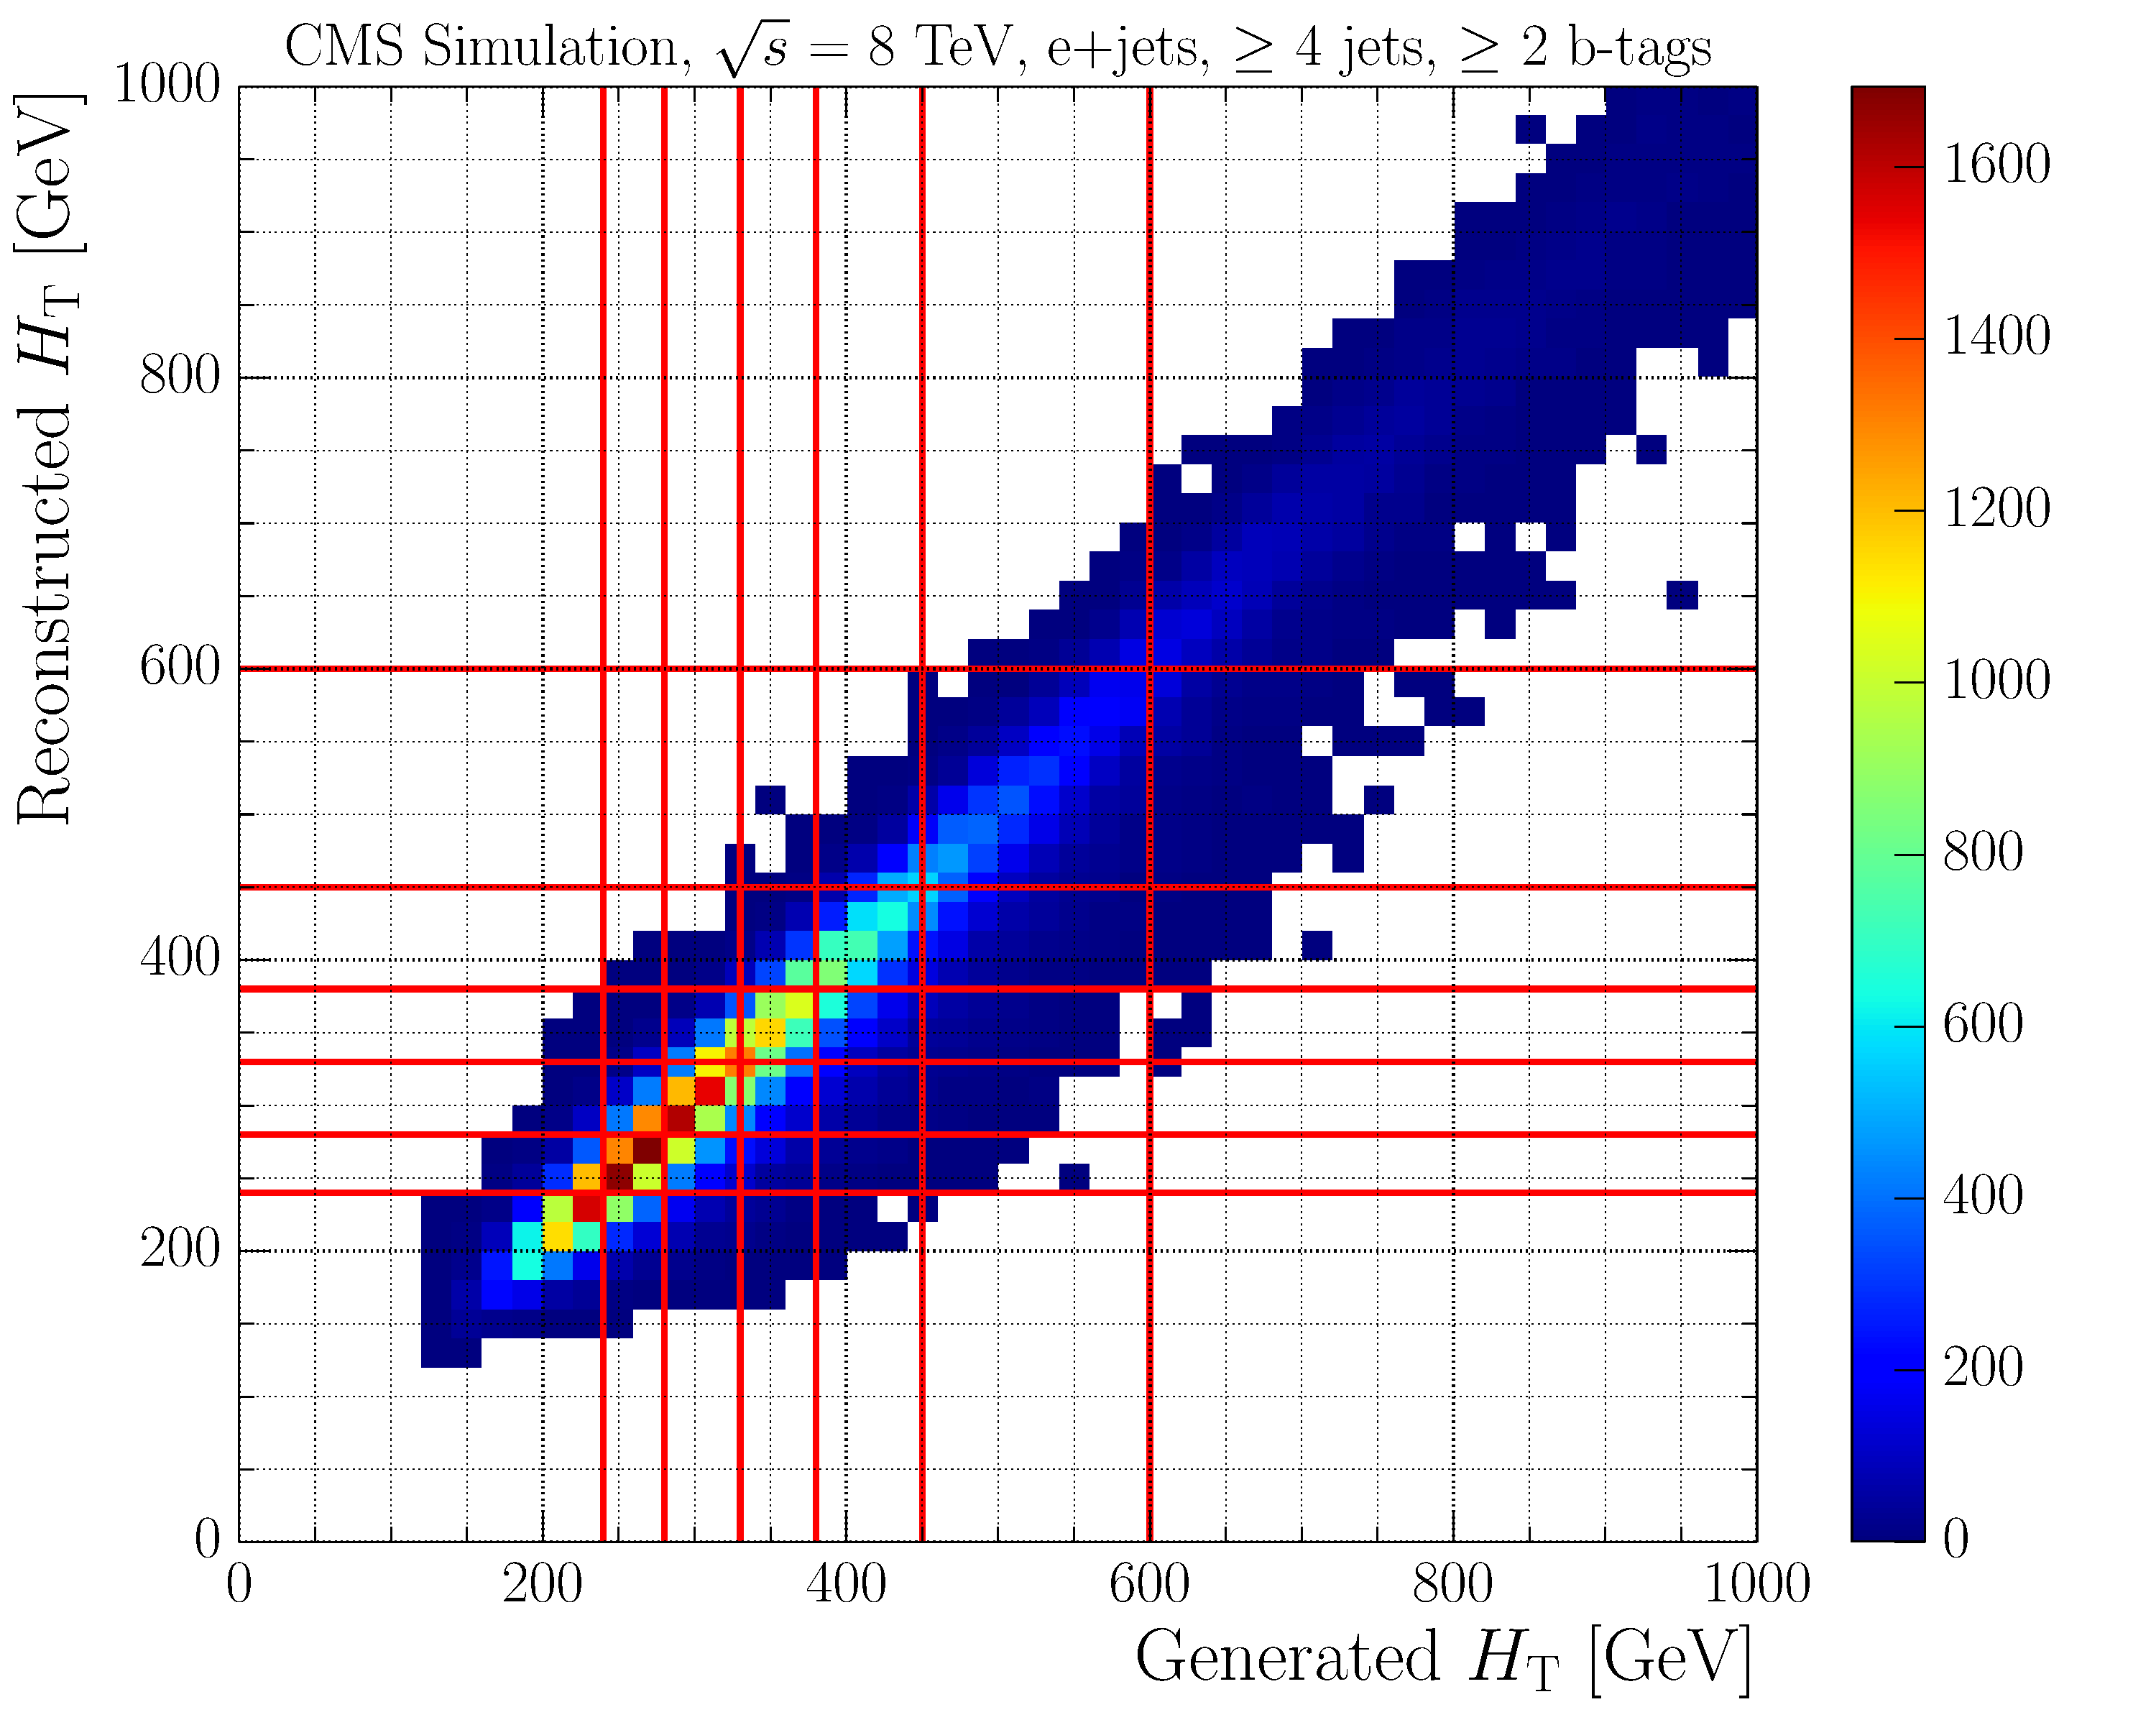
\includegraphics[width=0.5\textwidth]{binning/EPlusJets_HT}}\hfill
	\subfloat[]{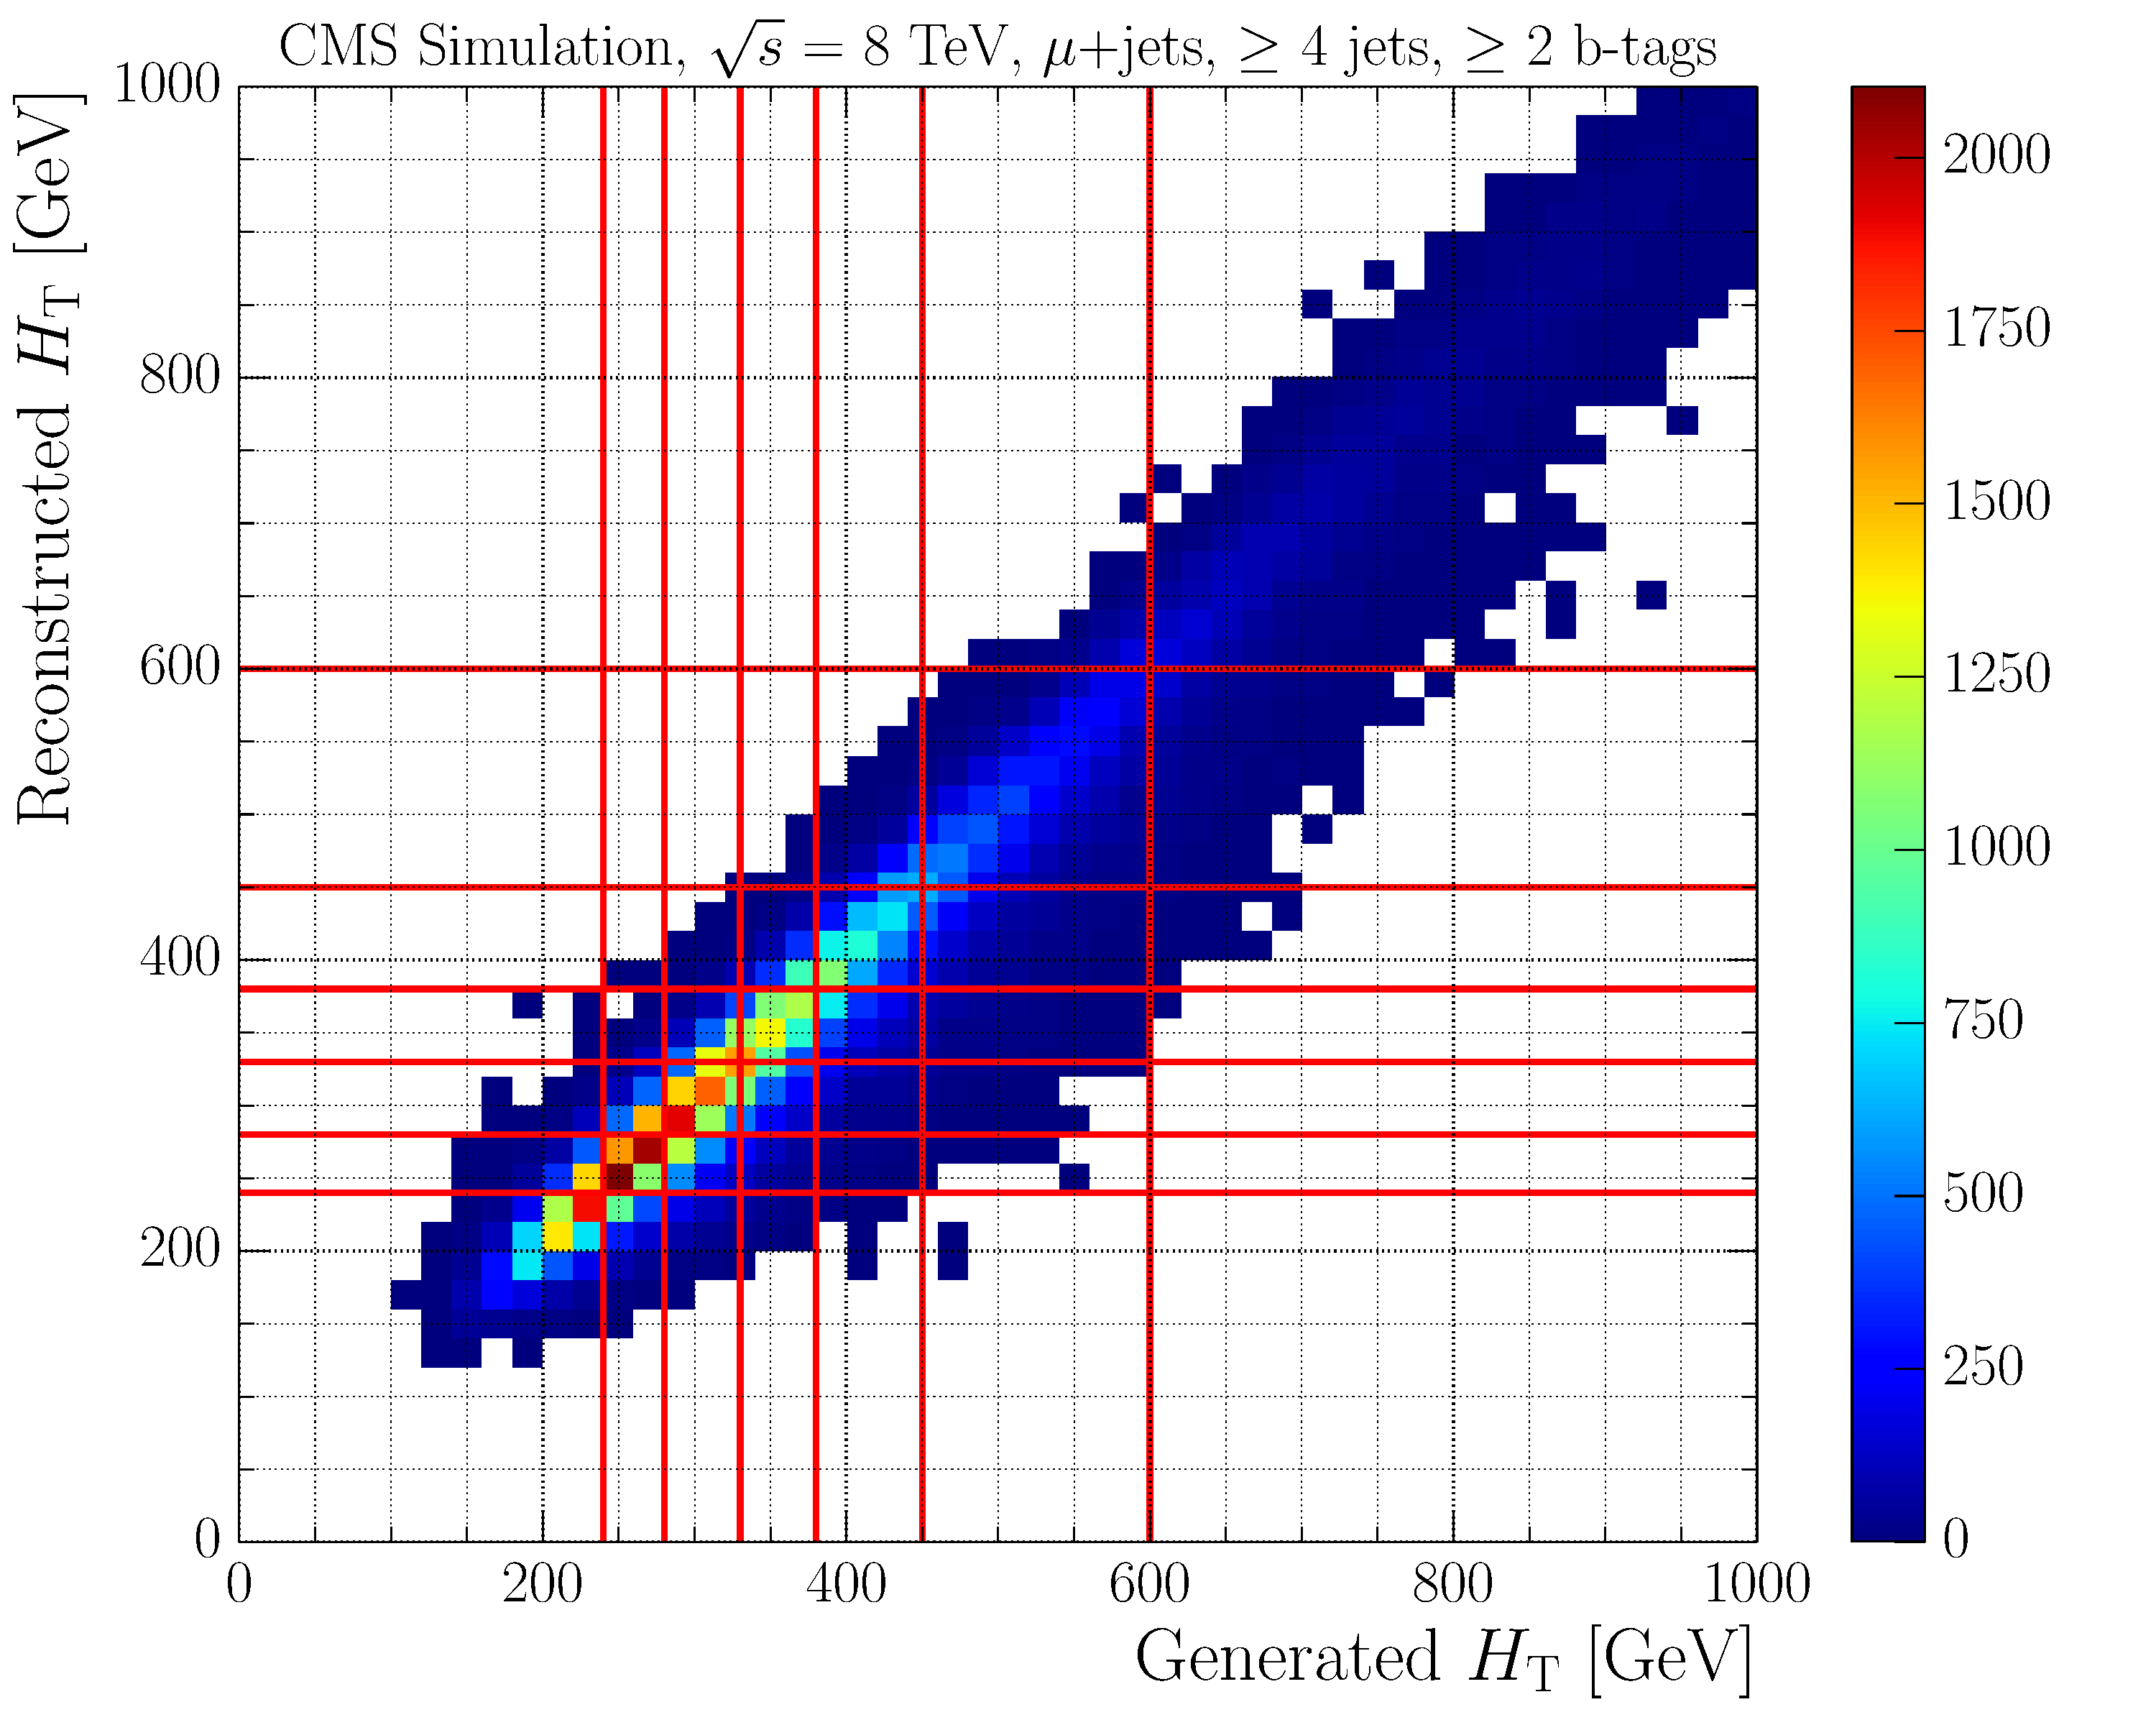
\includegraphics[width=0.5\textwidth]{binning/MuPlusJets_HT}}\\ 
	%ST
	\subfloat[]{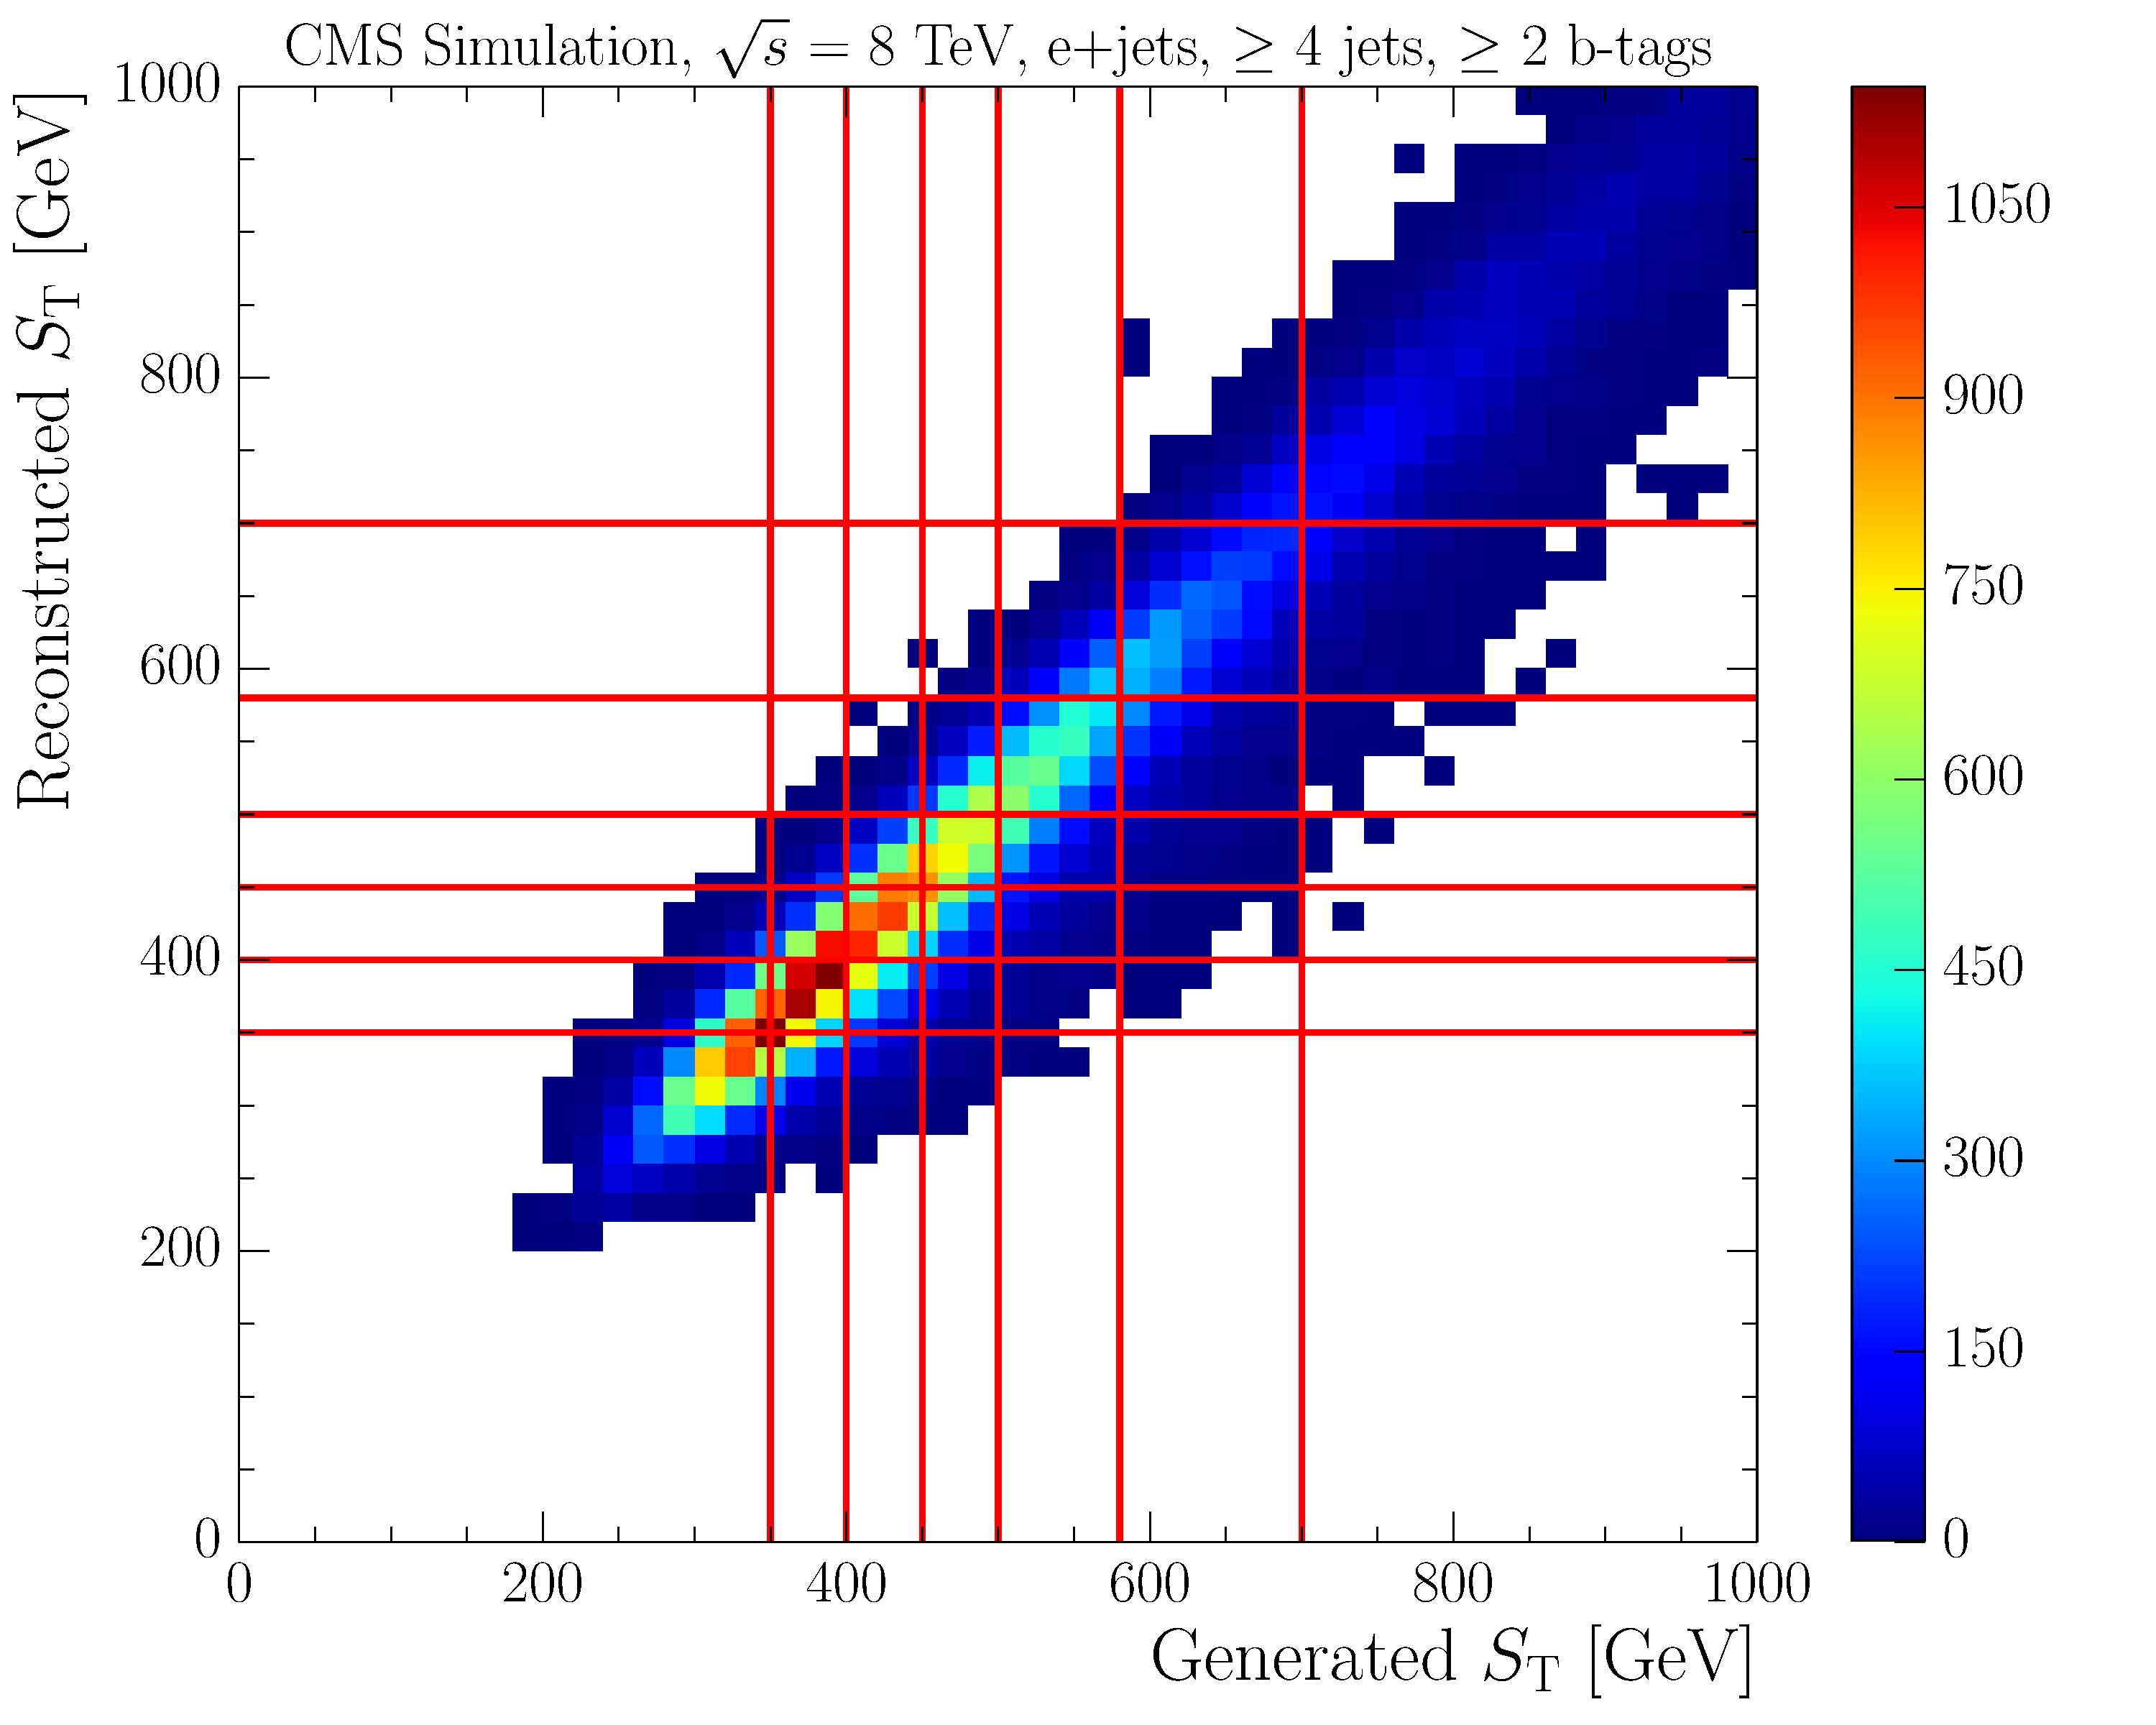
\includegraphics[width=0.5\textwidth]{binning/EPlusJets_ST}}\hfill
	\subfloat[]{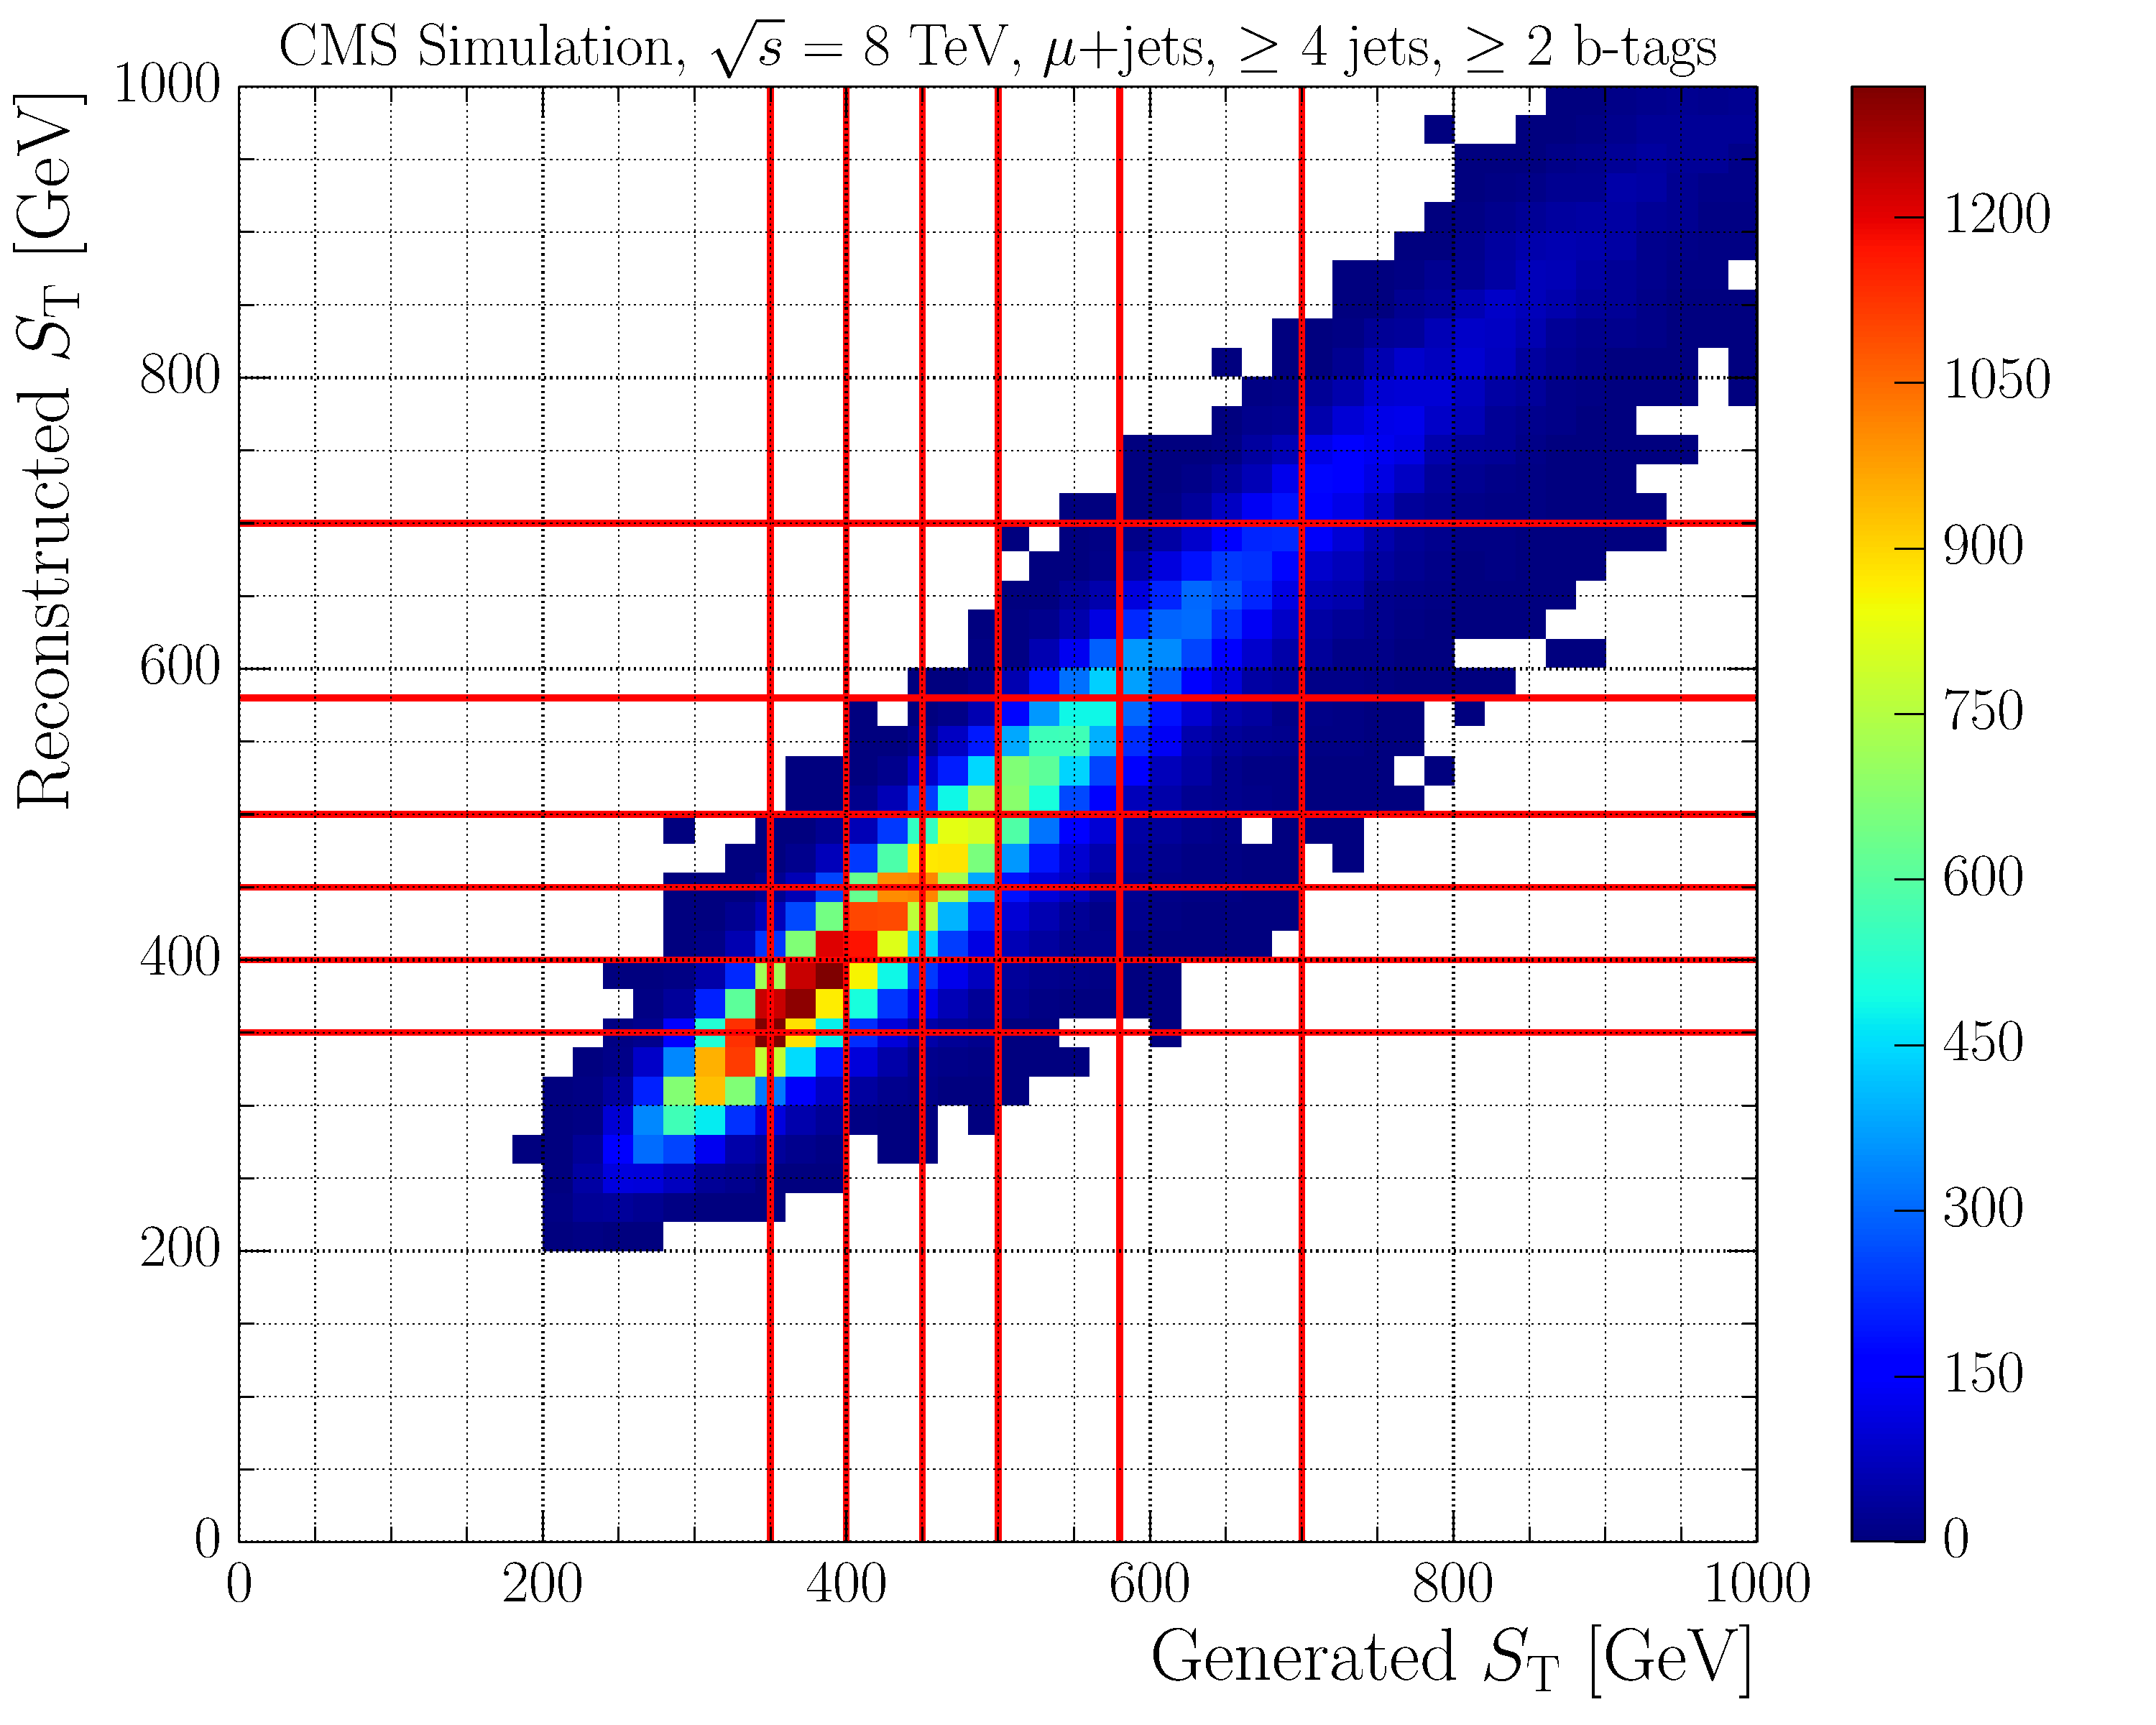
\includegraphics[width=0.5\textwidth]{binning/MuPlusJets_ST}}\\ 
    \caption[Reconstructed versus generated \HT and \ST]{Reconstructed versus generated \HT (a, b) and \ST (c, d) for
    electron plus jets (left) and muon plus jets events (right).}
	\label{fig:choice_of_bins_appendix_1}
 \end{figure}

 \begin{figure}[hbtp]
	\centering
	%WPT
	\subfloat[]{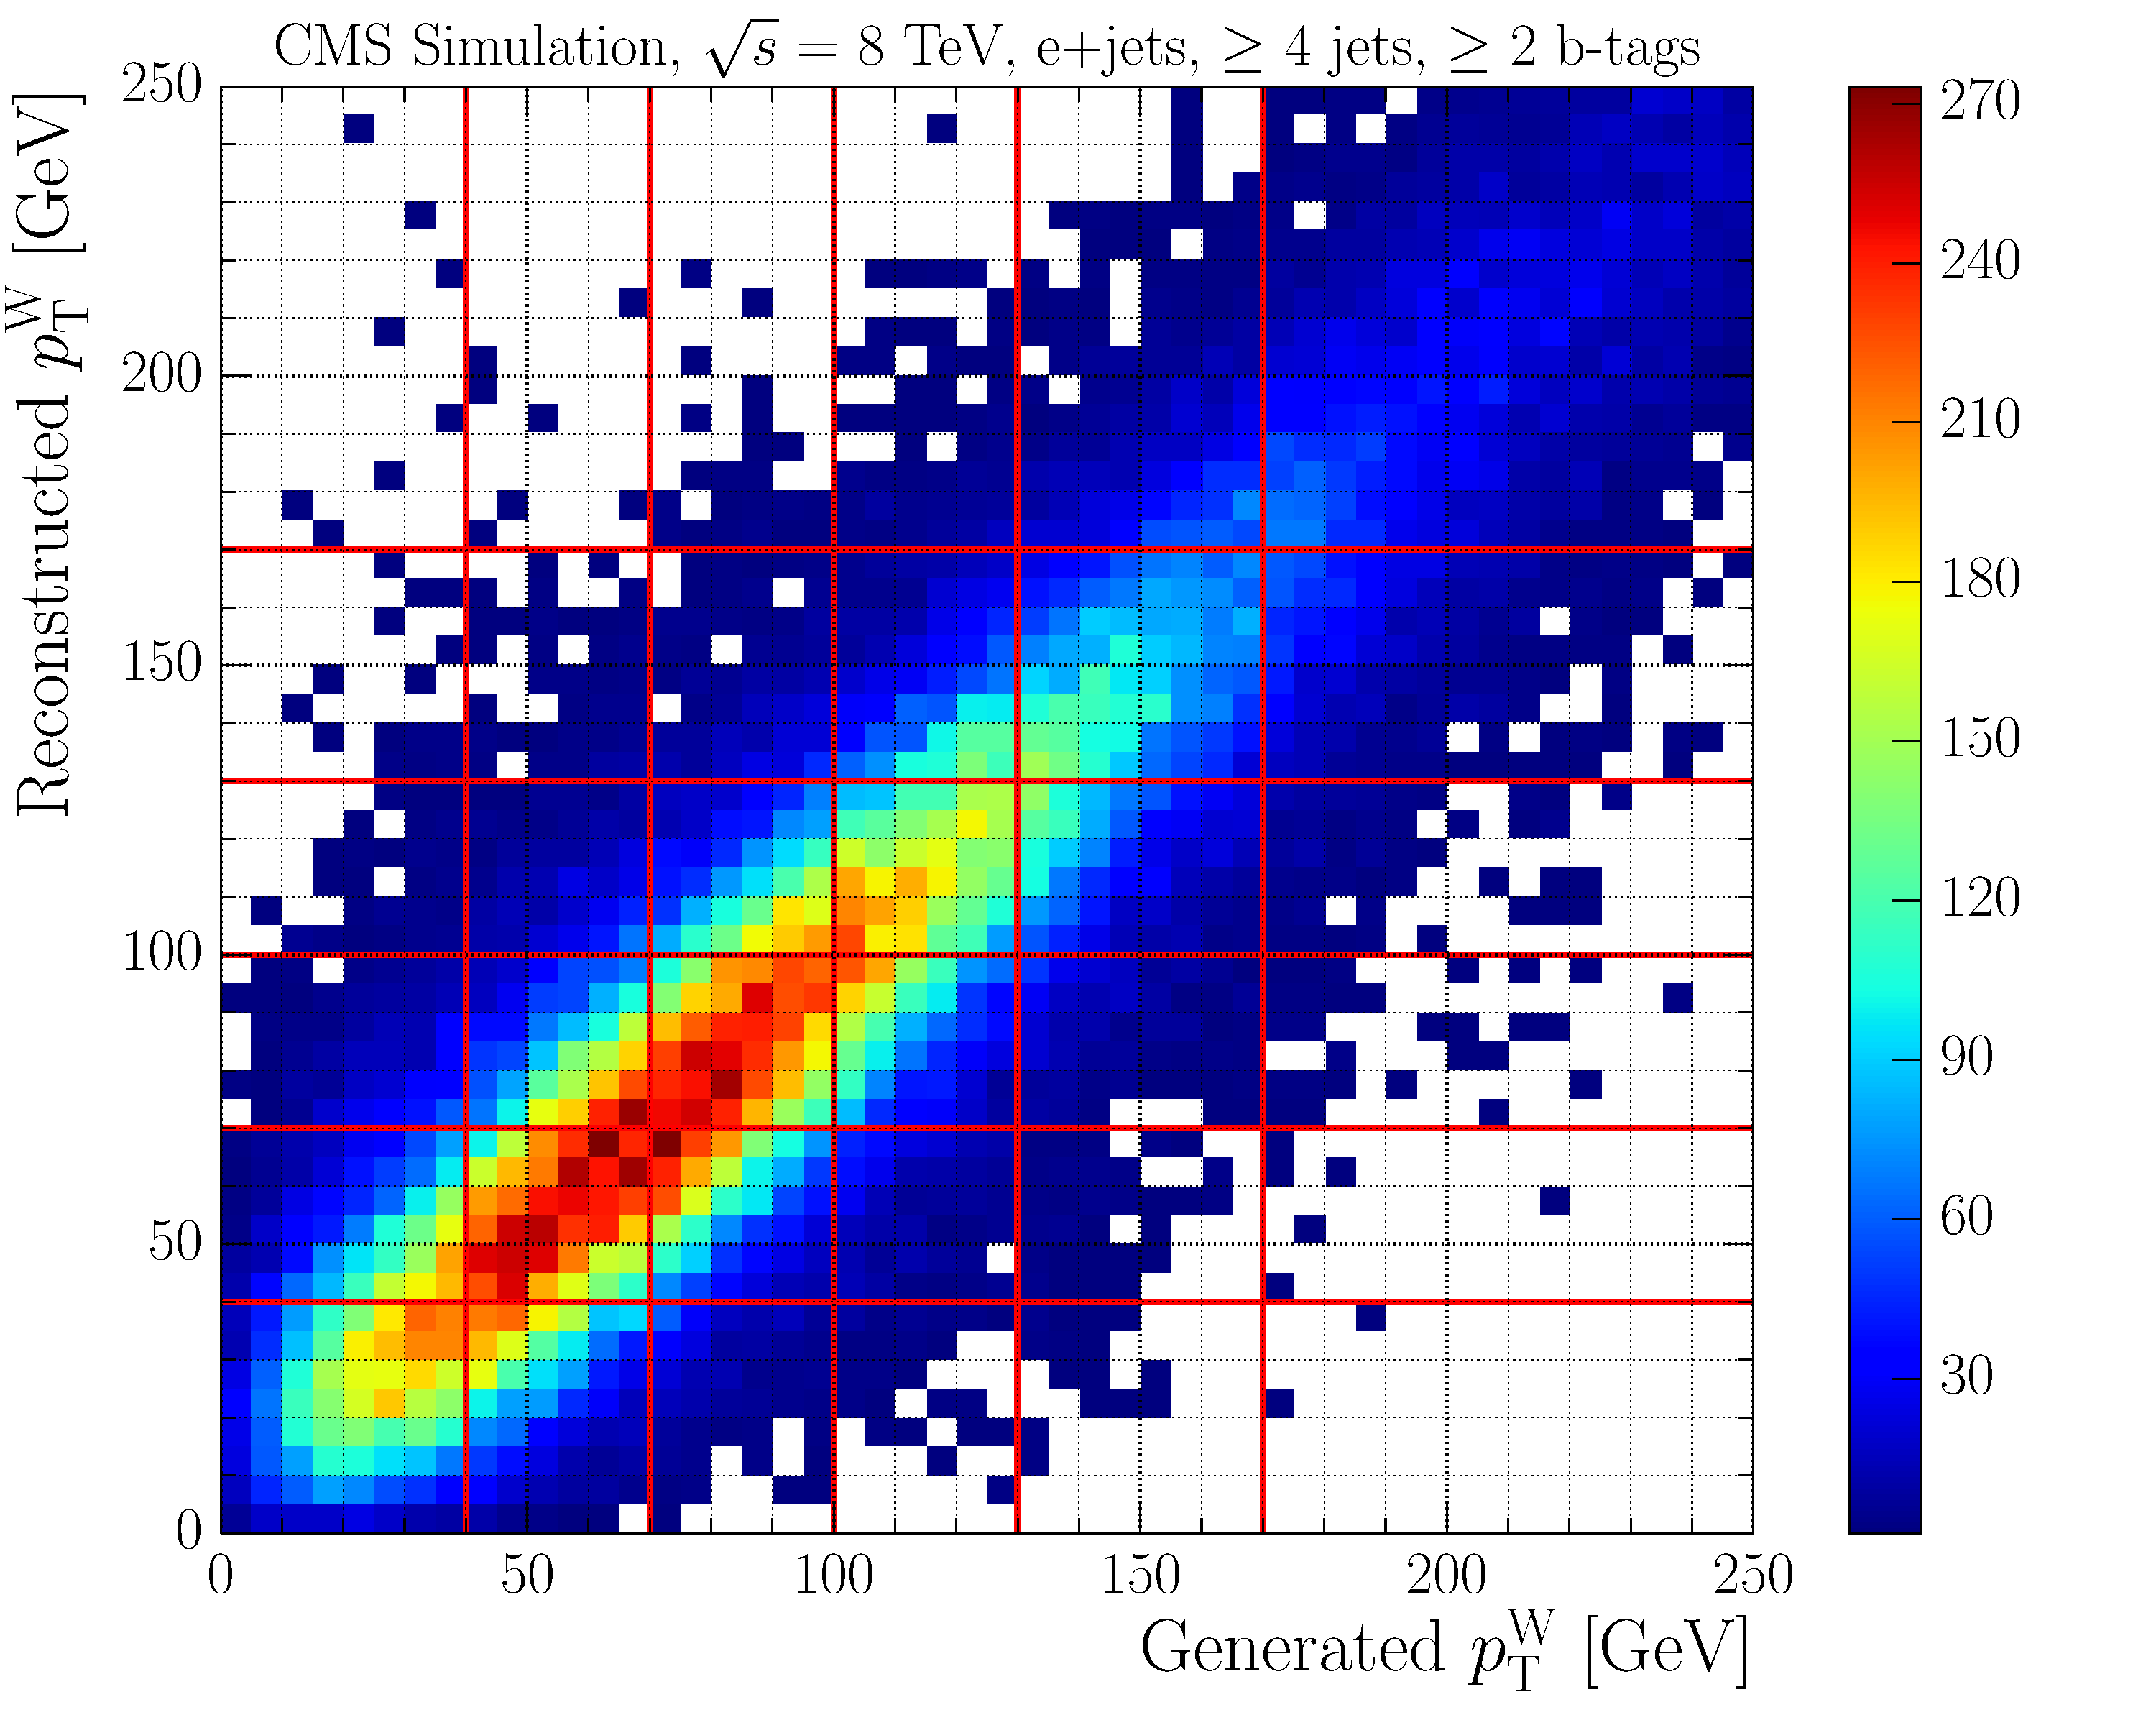
\includegraphics[width=0.5\textwidth]{binning/EPlusJets_WPT}}\hfill
	\subfloat[]{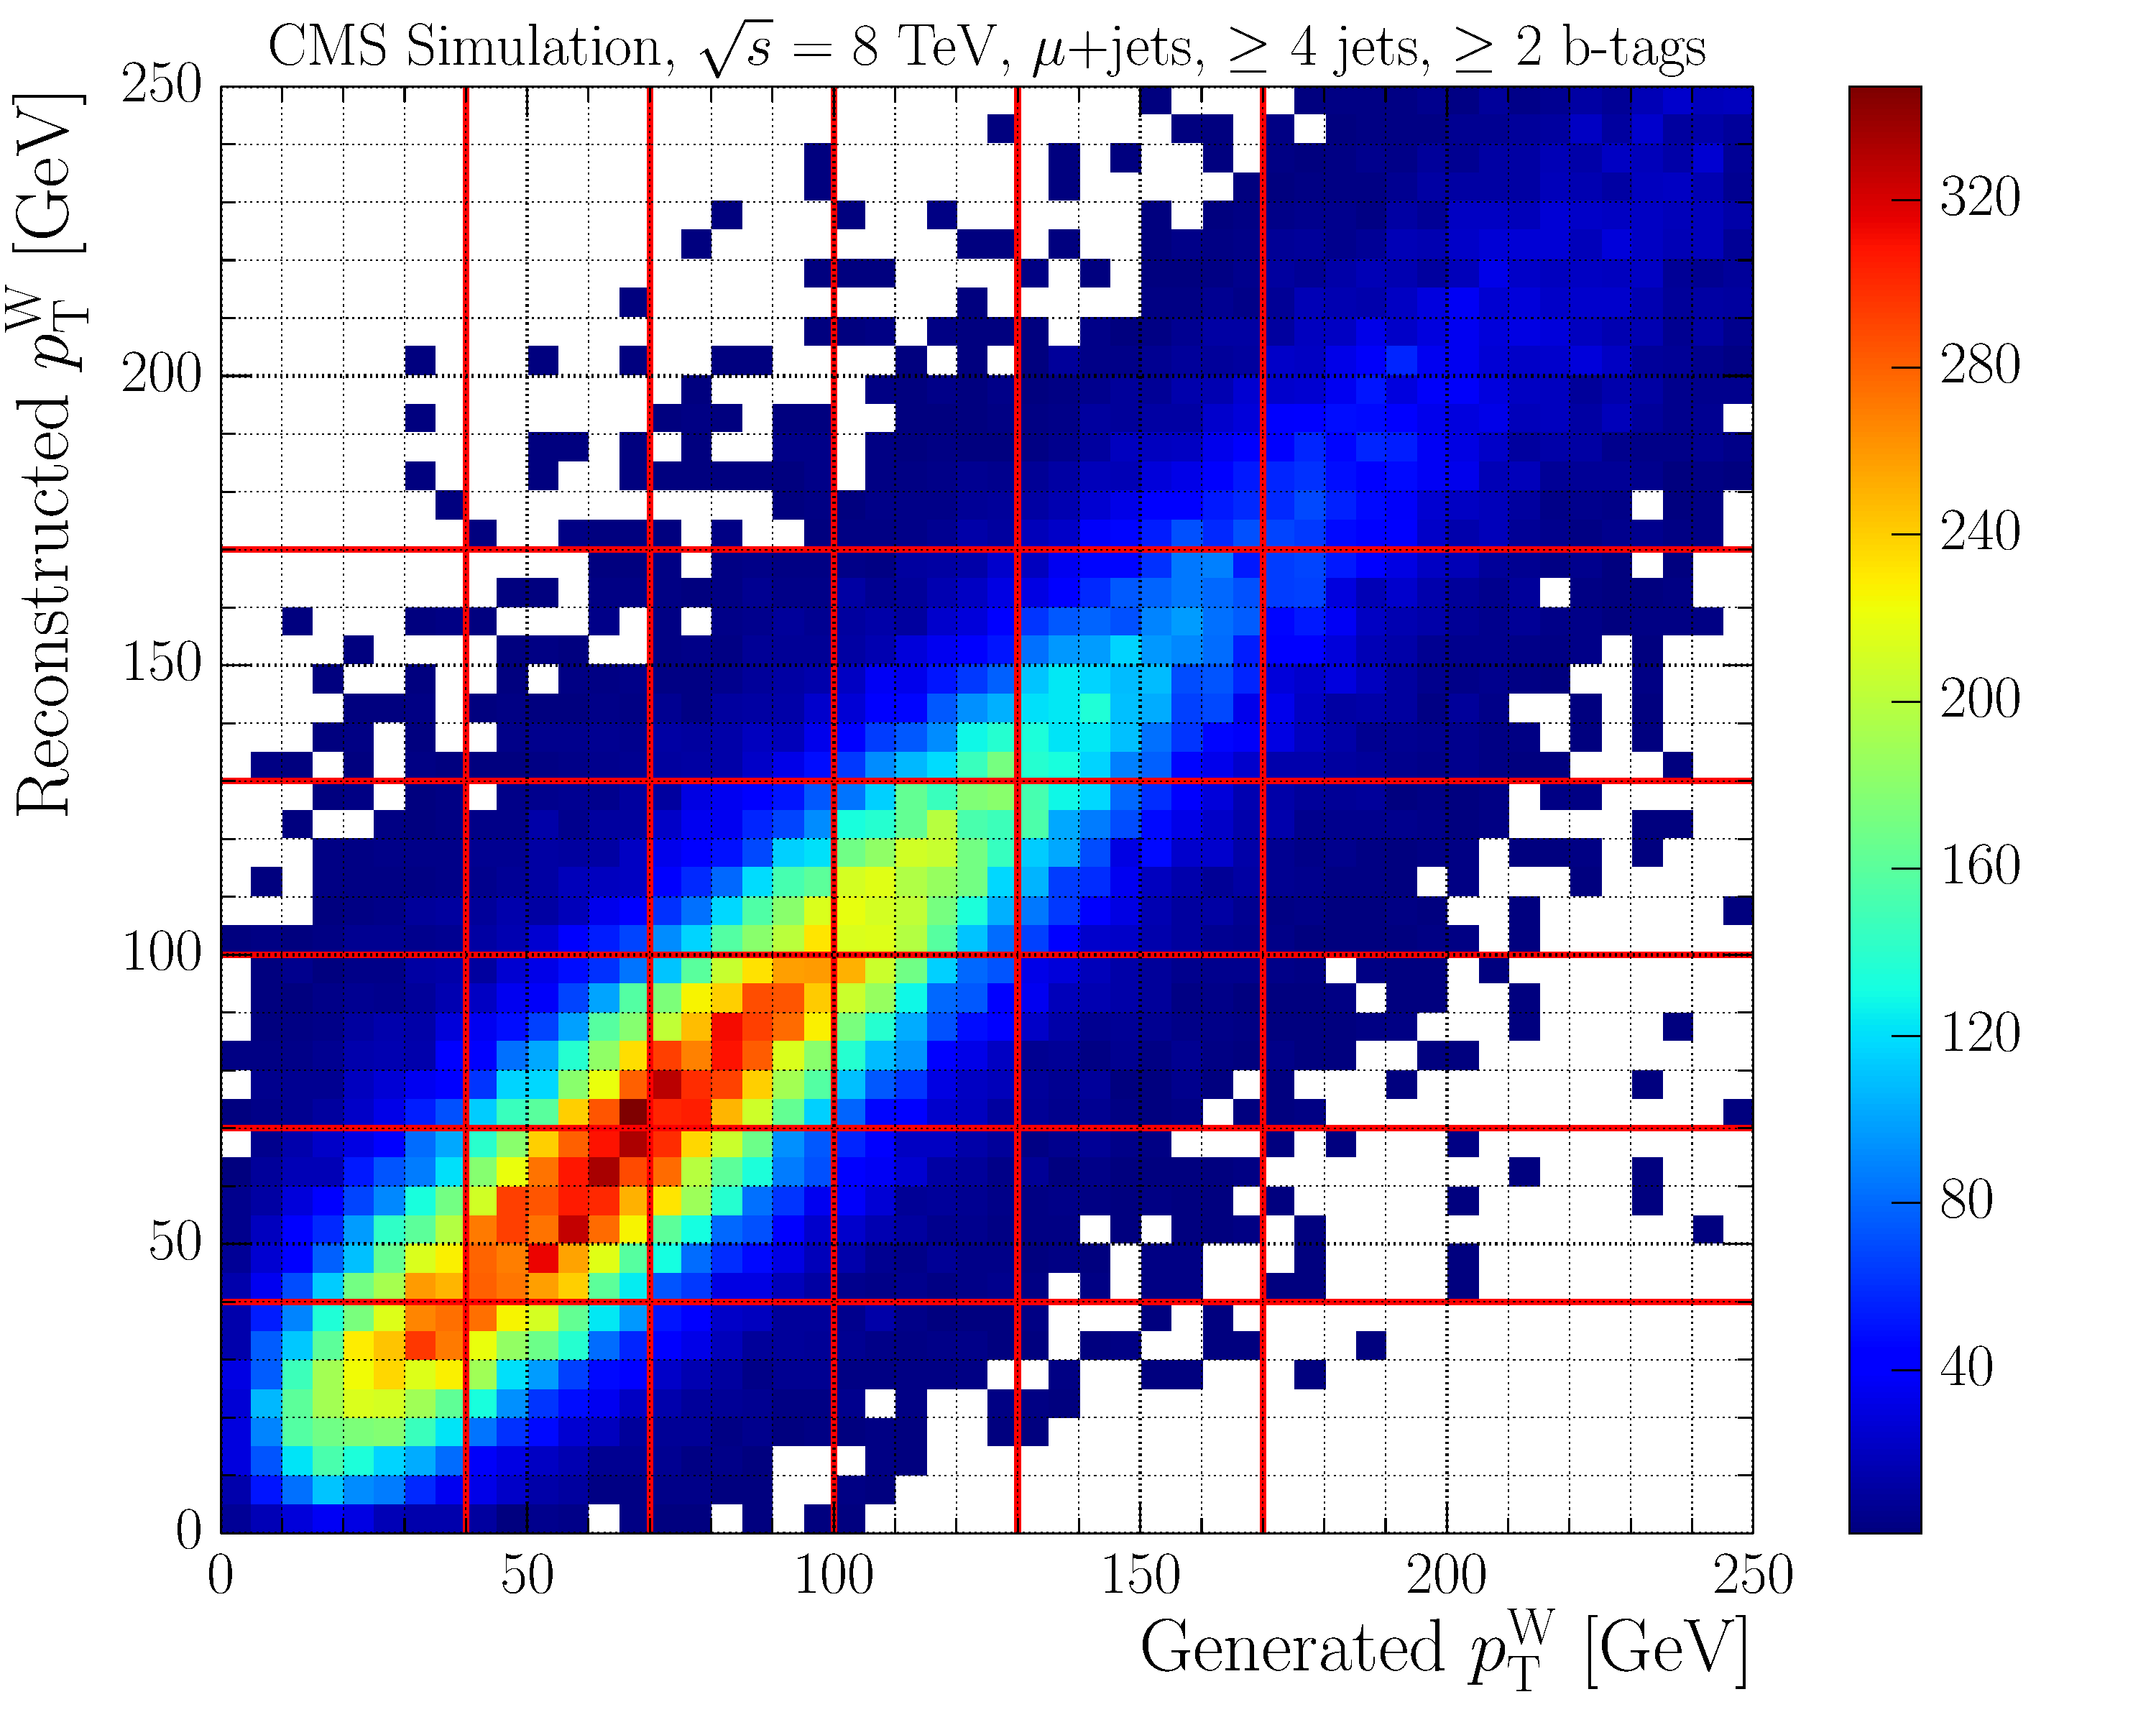
\includegraphics[width=0.5\textwidth]{binning/MuPlusJets_WPT}}\\
	%MT
	\subfloat[]{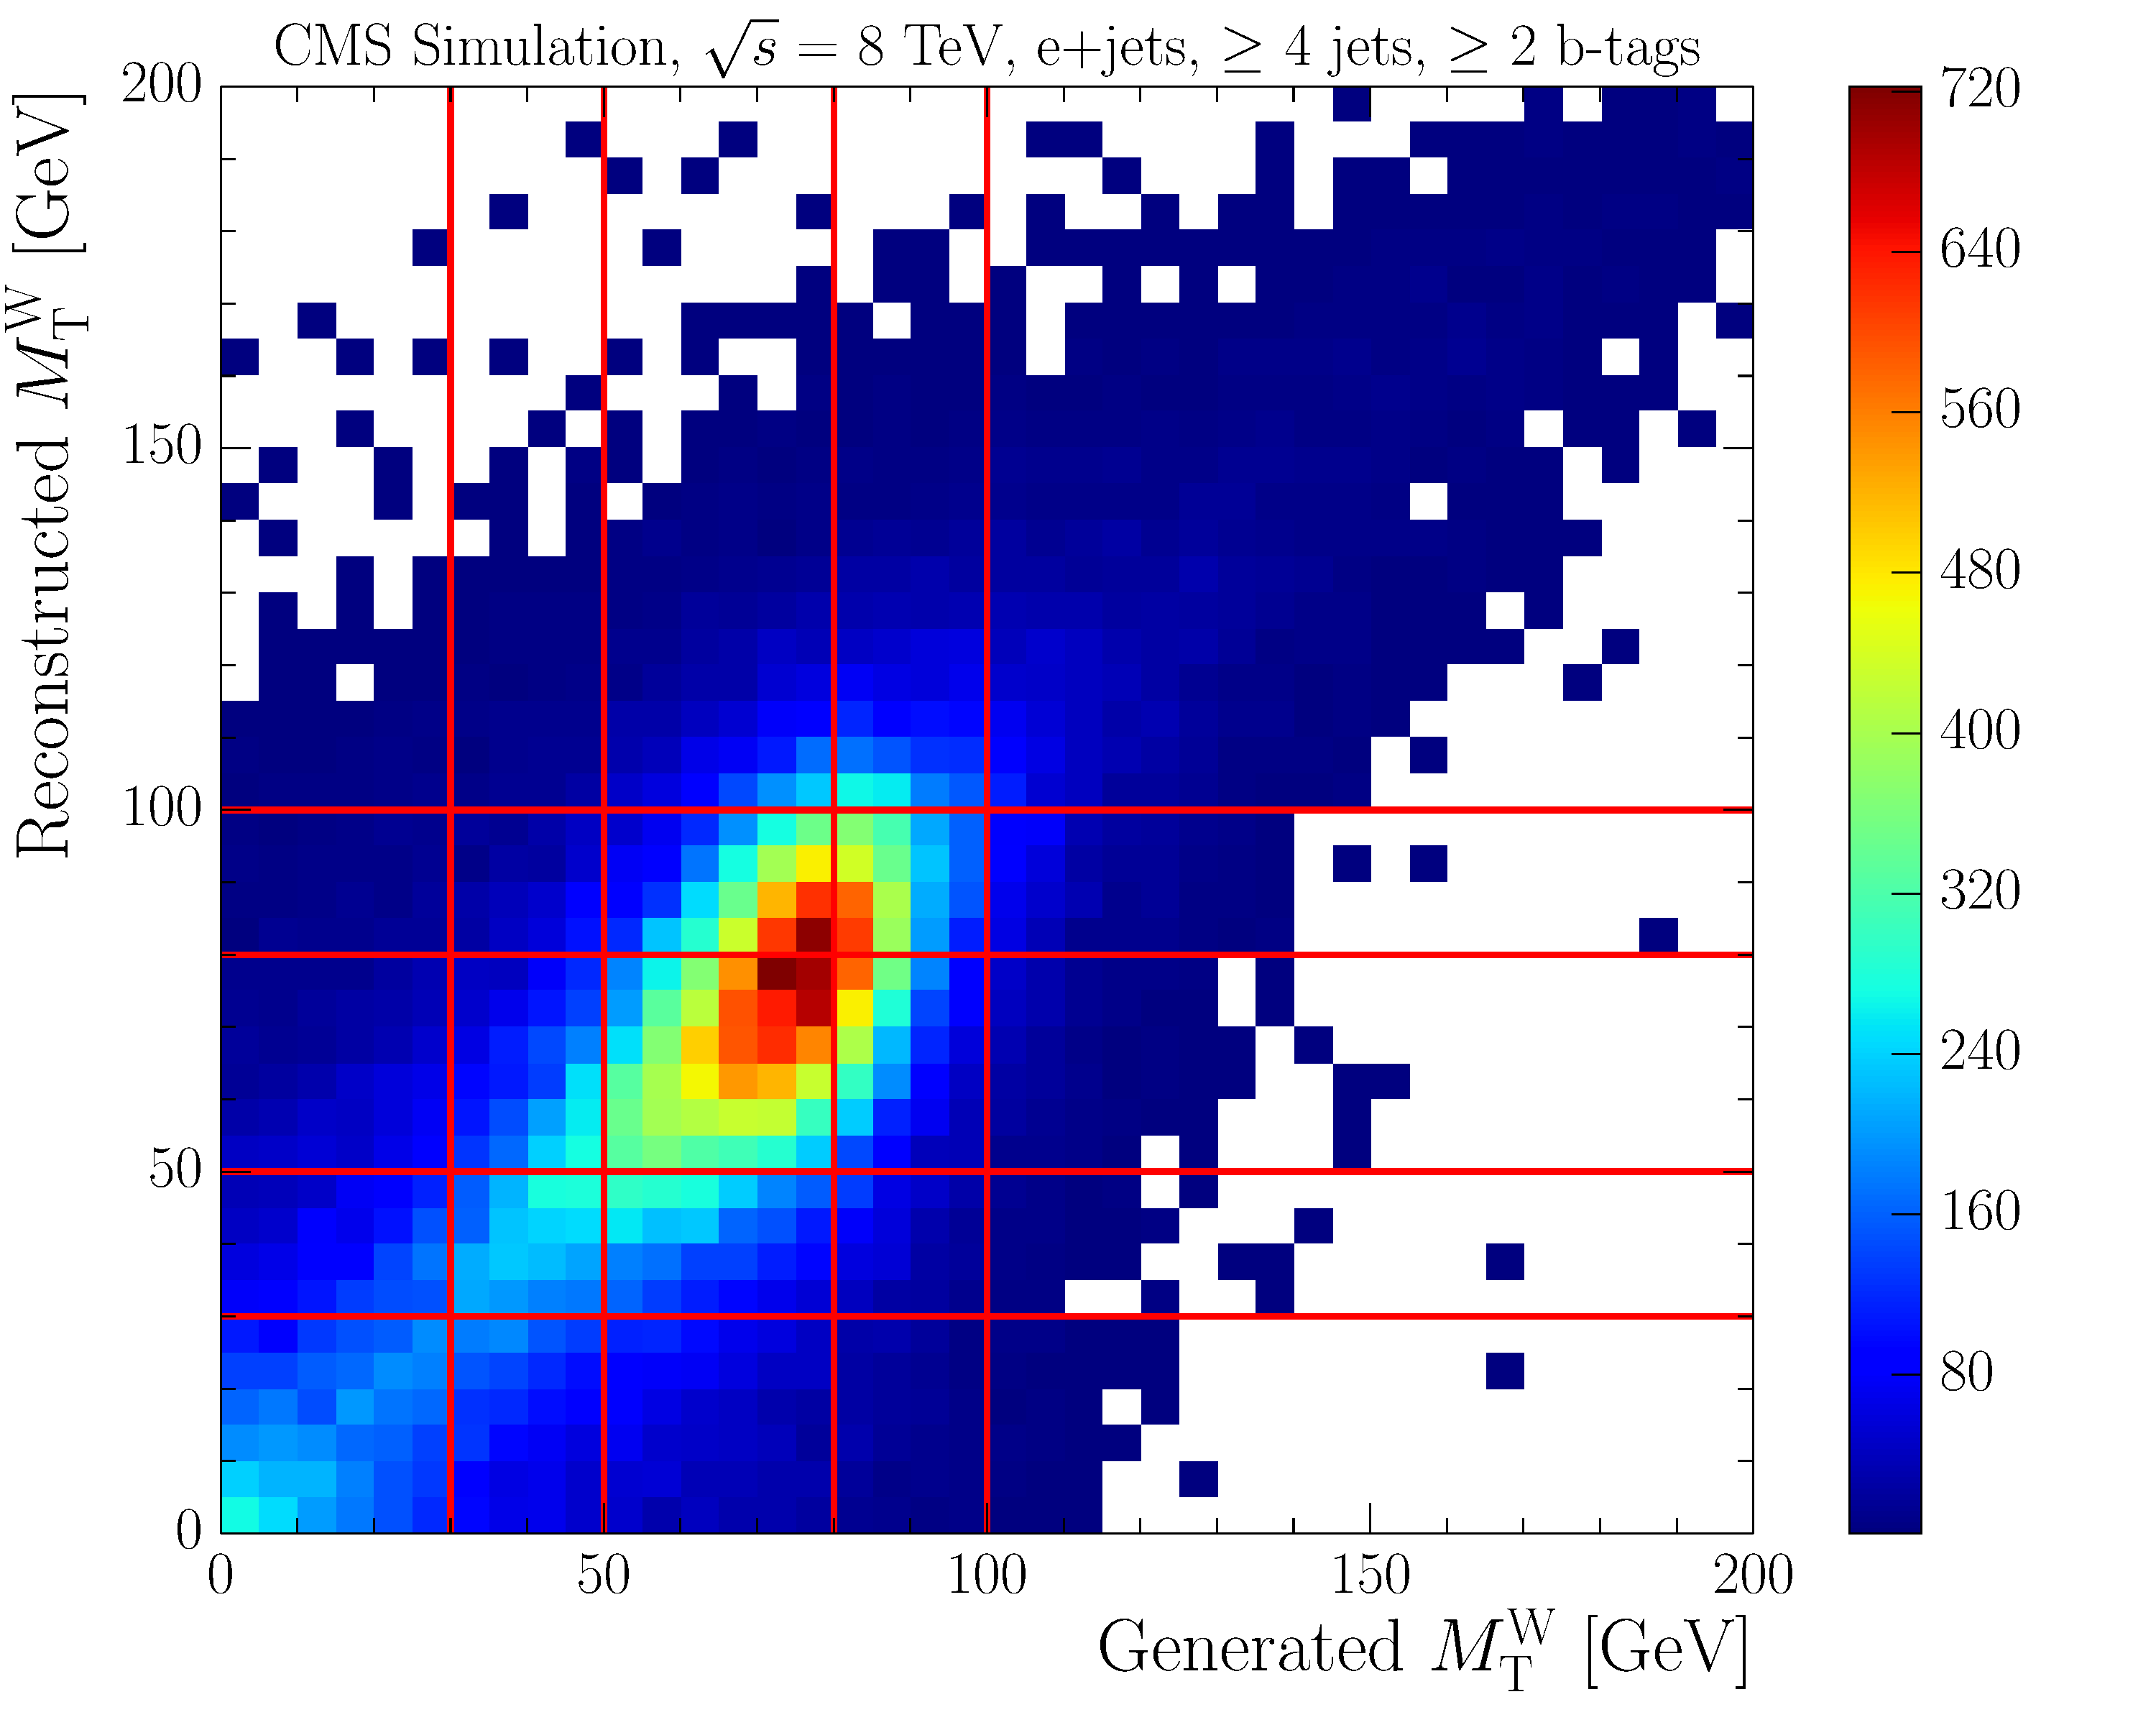
\includegraphics[width=0.5\textwidth]{binning/EPlusJets_MT}}\hfill
	\subfloat[]{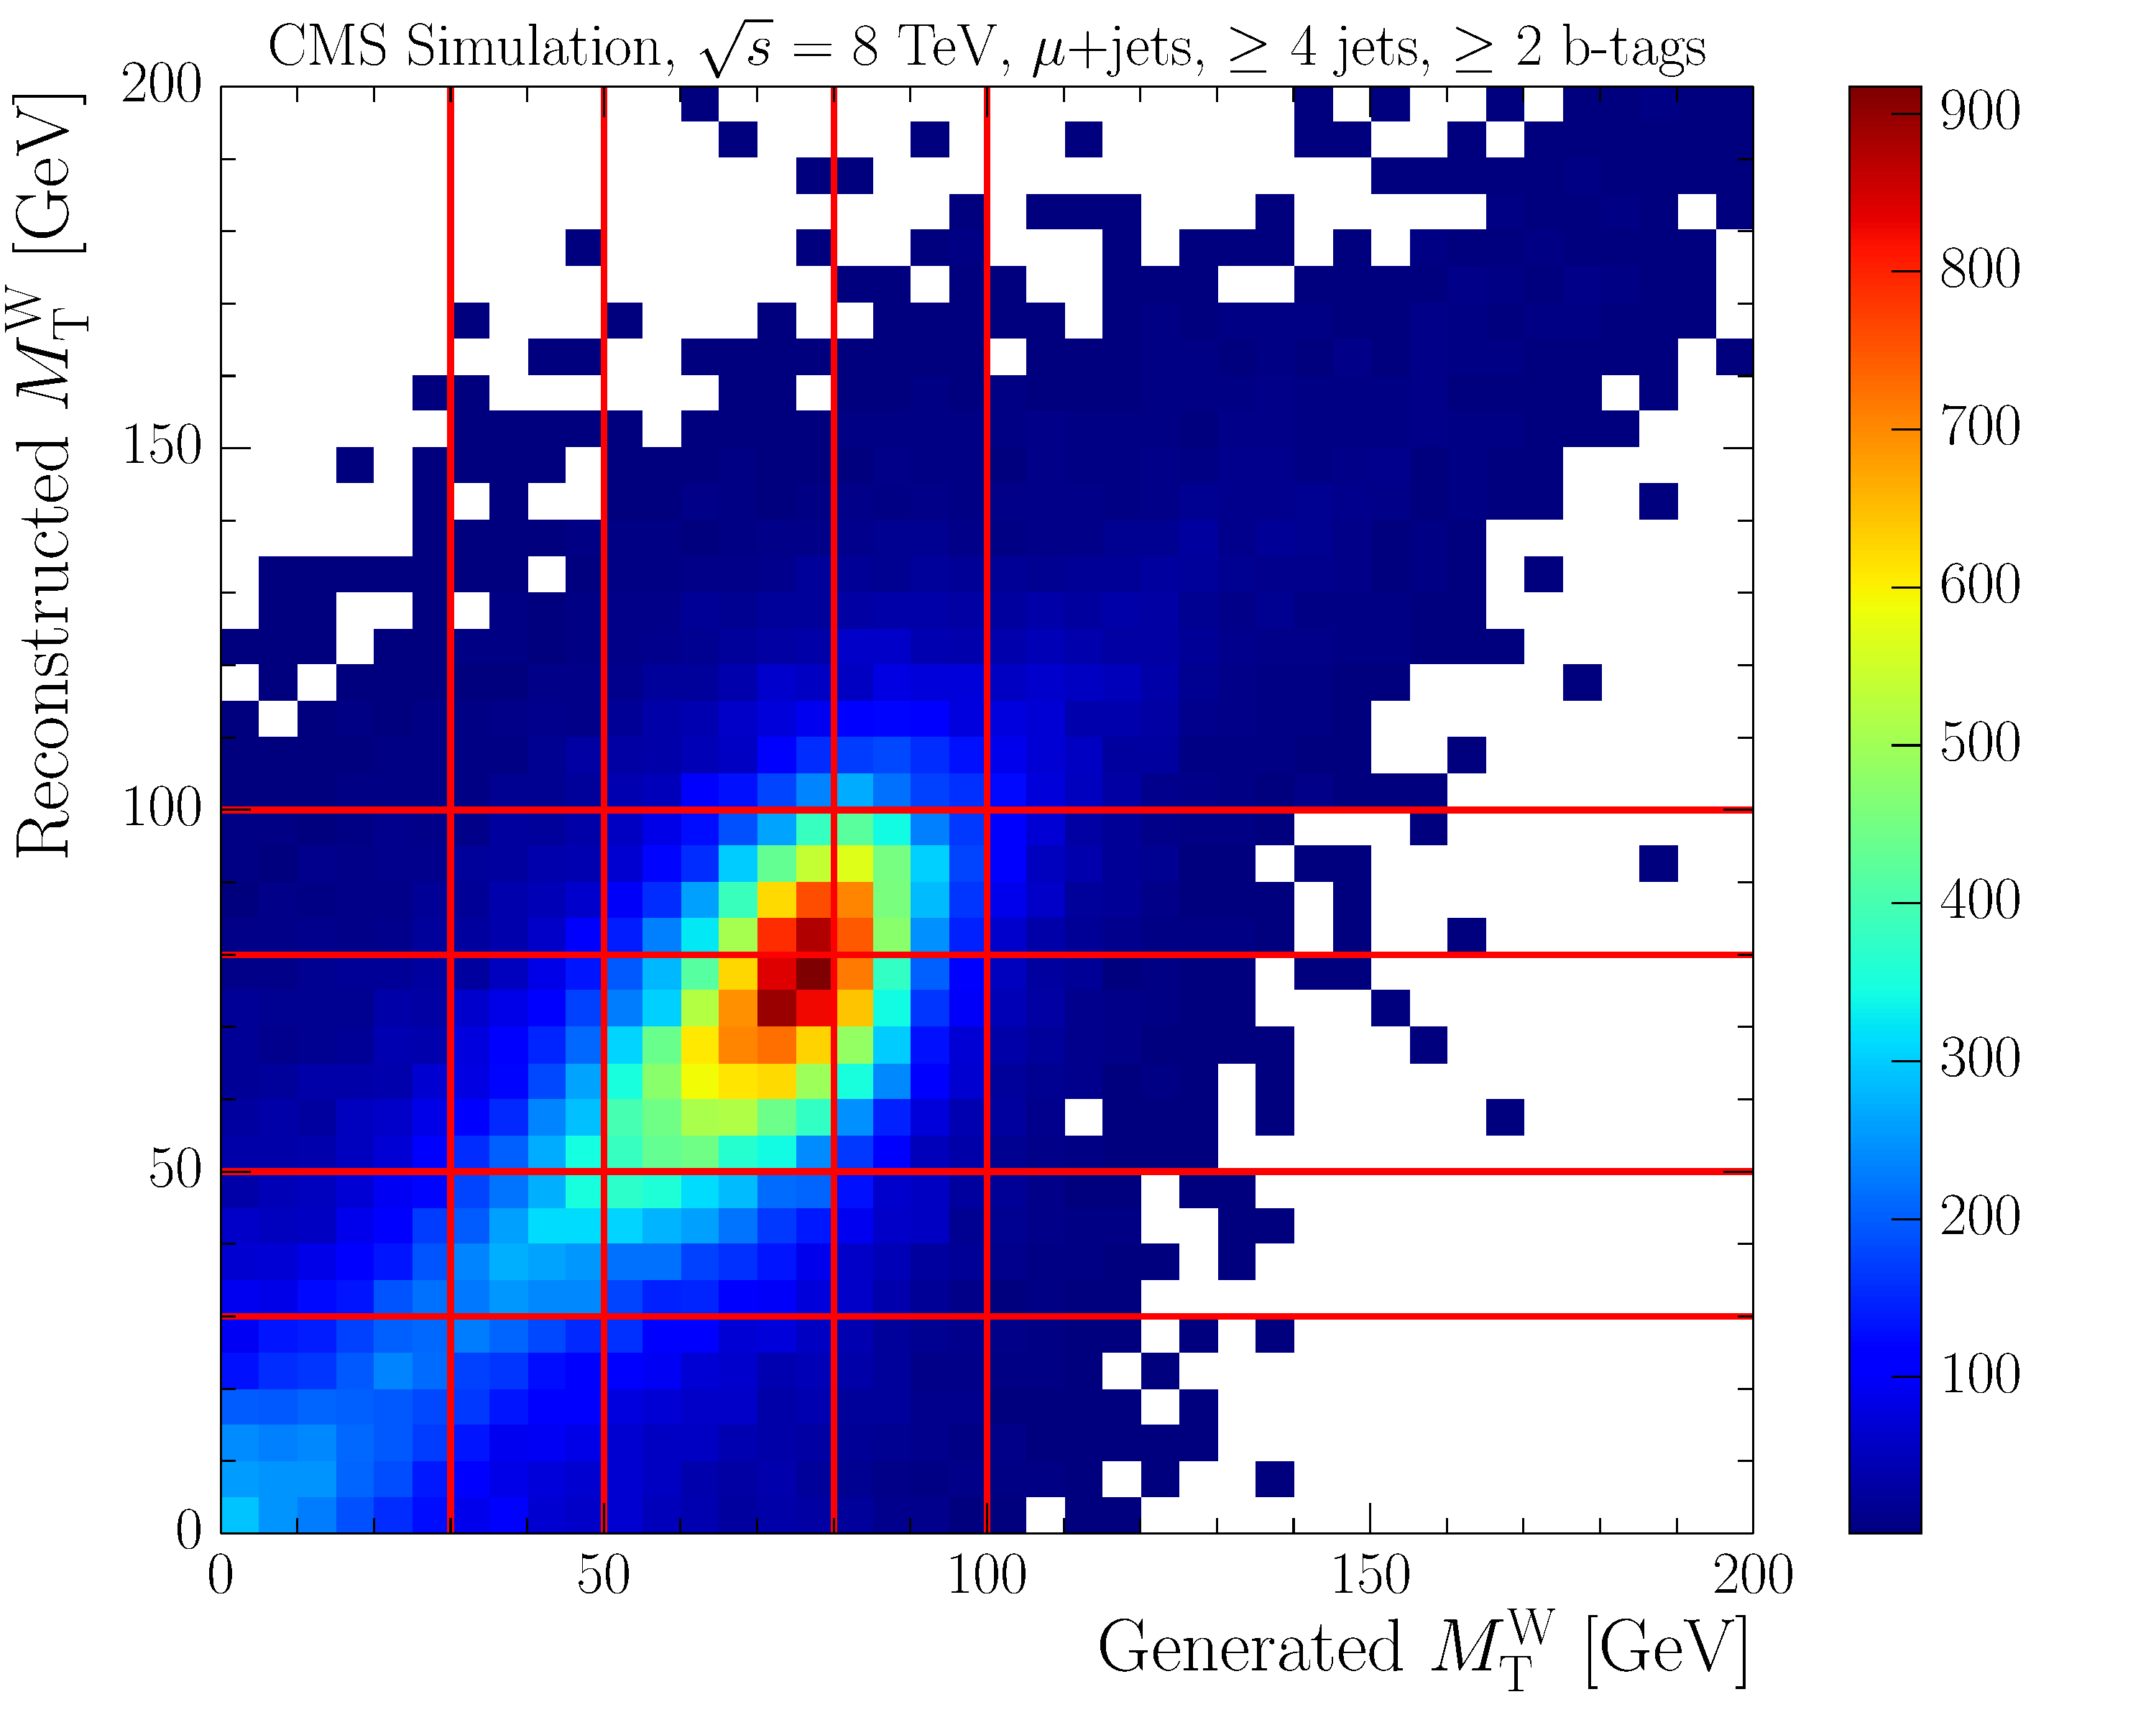
\includegraphics[width=0.5\textwidth]{binning/MuPlusJets_MT}}\\
    \caption[Reconstructed versus generated \WPT and \MT]{Reconstructed versus generated \WPT (a, b) and \MT (c, d) for
    electron plus jets (left) and muon plus jets events (right).}
	\label{fig:choice_of_bins_appendix_2}
 \end{figure}

\newpage


\begin{table}[htbp]
  	\centering
  	\caption{Stability and purity of chosen \HT bins in the electron channel for \ttbar MC events.}
  	\label{tab:binning_HT_electron}
	\resizebox{\columnwidth}{!}{
	\begin{tabular}{|l|r|r|r|r|r|r|r|}
	\toprule
	bin & $80 < \HT < 240$ & $240 \leq \HT <280$ & $280 \leq \HT < 330$ & $330 \leq \HT < 380$ & $380 \leq \HT < 450$ & $450 \leq \HT < 600$ & $\HT \geq 600$ \\
	\midrule 
	events & 10601 & 12569 & 14372 & 12397 & 10893 & 10721 & 5609\\
	purity & 0.82 & 0.62 & 0.63 & 0.62 & 0.68 & 0.81 & 0.9\\
	stability &  0.76 & 0.63 & 0.65 & 0.64 & 0.68 & 0.8 & 0.9\\
	\bottomrule
	\end{tabular}
	}
\end{table}


\begin{table}[htbp]
  	\centering
  	\caption{Stability and purity of chosen \HT bins in the muon channel for \ttbar MC events.}
  	\label{tab:binning_HT_muon}
	\resizebox{\columnwidth}{!}{
	\begin{tabular}{|l|r|r|r|r|r|r|r|}
	\toprule
	bin & $80 < \HT < 240$ & $240 \leq \HT <280$ & $280 \leq \HT < 330$ & $330 \leq \HT < 380$ & $380 \leq \HT < 450$ & $450 \leq \HT < 600$ & $\HT \geq 600$ \\
	\midrule 
	events & 12337 & 14821 & 16747 & 14268 & 12258 & 12119 & 5857\\
	purity & 0.82 & 0.63 & 0.64 & 0.63 & 0.67 & 0.81 & 0.9\\
	stability & 0.76 & 0.64 & 0.65 & 0.65 & 0.68 & 0.81 & 0.89\\
	\bottomrule
	\end{tabular}
	}
\end{table}



\begin{table}[htbp]
  	\centering
  	\caption{Stability and purity of chosen \ST bins in the electron channel for \ttbar MC events.}
  	\label{tab:binning_ST_electron}
	\resizebox{\columnwidth}{!}{
	\begin{tabular}{|l|r|r|r|r|r|r|r|}
	\toprule
	bin & $106 < \ST < 350$ & $ 350 \leq \ST < 400$ & $400 \leq \ST < 450$ & $450 \leq \ST < 500$ & $500 \leq \ST < 580$ & $580 \leq \ST < 700$ & $\ST \geq 700$ \\
	\midrule 
	events & 11183 & 13246 & 12073 & 10709 & 11317 & 9166 & 8373\\
	purity & 0.83 & 0.6 & 0.53 & 0.53 & 0.63 & 0.71 & 0.87\\
	stability & 0.73 & 0.6 & 0.55 & 0.55 & 0.66 & 0.73 & 0.91\\ 
	\bottomrule
	\end{tabular}
	}
\end{table}


\begin{table}[htbp]
  	\centering
  	\caption{Stability and purity of chosen \ST bins in the muon channel for \ttbar MC events.}
  	\label{tab:binning_ST_muon}
	\resizebox{\columnwidth}{!}{
	\begin{tabular}{|l|r|r|r|r|r|r|r|}
	\toprule
	bin & $106 < \ST < 350$ & $ 350 \leq \ST < 400$ & $400 \leq \ST < 450$ & $450 \leq \ST < 500$ & $500 \leq \ST < 580$ & $580 \leq \ST < 700$ & $\ST \geq 700$ \\
	\midrule 
	events & 13593 & 15717 & 13878 & 12307 & 12732 & 10135 & 8875\\
	purity &  0.83 & 0.61 & 0.54 & 0.54 & 0.64 & 0.71 & 0.87\\
	stability & 0.74 & 0.61 & 0.55 & 0.56 & 0.66 & 0.74 & 0.9\\
	\bottomrule
	\end{tabular}
	}
\end{table}


\begin{table}[htbp]
  	\centering
  	\caption{Stability and purity of chosen \WPT bins in the electron channel for \ttbar MC events.}
  	\label{tab:binning_WPT_electron}
	\resizebox{\columnwidth}{!}{
	\begin{tabular}{|l|r|r|r|r|r|r|}
	\toprule
	bin & $0 < \WPT < 40$ & $40 \leq \WPT < 70$ & $70 \leq \WPT < 100$ & $100 \leq \WPT < 130$ & $130 \leq \WPT < 170$ & $\WPT \geq 170$ \\
	\midrule 
	events &  10005 & 15849 & 16053 & 12203 & 9532 & 7717\\
	purity & 0.64 & 0.54 & 0.52 & 0.5 & 0.56 & 0.77\\
	stability & 0.63 & 0.54 & 0.52 & 0.51 & 0.57 & 0.76\\
	\bottomrule
	\end{tabular}
	}
\end{table}


\begin{table}[htbp]
  	\centering
  	\caption{Stability and purity of chosen \WPT bins in the muon channel for \ttbar MC events.}
  	\label{tab:binning_WPT_muon}
	\resizebox{\columnwidth}{!}{
	\begin{tabular}{|l|r|r|r|r|r|r|}
	\toprule
	bin & $0 < \WPT < 40$ & $40 \leq \WPT < 70$ & $70 \leq \WPT < 100$ & $100 \leq \WPT < 130$ & $130 \leq \WPT < 170$ & $\WPT \geq 170$ \\
	\midrule 
	events &  12379 & 18821 & 18330 & 13495 & 10260 & 8394 \\
	purity & 0.67 & 0.55 & 0.52 & 0.5 & 0.55 & 0.76\\
	stability & 0.63 & 0.55 & 0.53 & 0.51 & 0.56 & 0.76\\
	\bottomrule
	\end{tabular}
	}
\end{table}


\begin{table}[htbp]
  	\centering
  	\caption{Stability and purity of chosen \MT bins in the electron channel for \ttbar MC events.}
  	\label{tab:binning_MT_electron}
	\resizebox{\columnwidth}{!}{
	\begin{tabular}{|l|r|r|r|r|r|}
	\toprule
	bin & $0 < \MT < 30$ & $30 \leq \MT < 50$ & $50 \leq \MT < 80$ & $80 \leq \MT < 100$ & $MT \geq 100$ \\
	\midrule 
	events &  11509 & 11633 & 26288 & 14824 & 8921 \\
	purity & 0.57 & 0.35 & 0.65 & 0.4 & 0.36\\
	stability & 0.62 & 0.37 & 0.53 & 0.41 & 0.67\\
	\bottomrule
	\end{tabular}
	}
\end{table}


\begin{table}[htbp]
  	\centering
  	\caption{Stability and purity of chosen \MT bins in the muon channel for \ttbar MC events.}
  	\label{tab:binning_MT_muon}
	\resizebox{\columnwidth}{!}{
	\begin{tabular}{|l|r|r|r|r|r|}
	\toprule
	bin & $0 < \MT < 30$ & $30 \leq \MT < 50$ & $50 \leq \MT < 80$ & $80 \leq \MT < 100$ & $MT \geq 100$ \\
	\midrule 
	events & 13209 & 13636 & 30669 & 16974 & 9179.3\\
	purity & 0.56 & 0.36 & 0.66 & 0.42 & 0.37\\
	stability & 0.64 & 0.38 & 0.54 & 0.42 & 0.66\\
	\bottomrule
	\end{tabular}
	}
\end{table}

\chapter{Fitting templates}
\label{a:templates}

\sisetup{range-phrase = --}
\sisetup{range-units = single}

\centering
\section*{\HT variable}

\begin{figure}[!htbp]
	\centering
  	{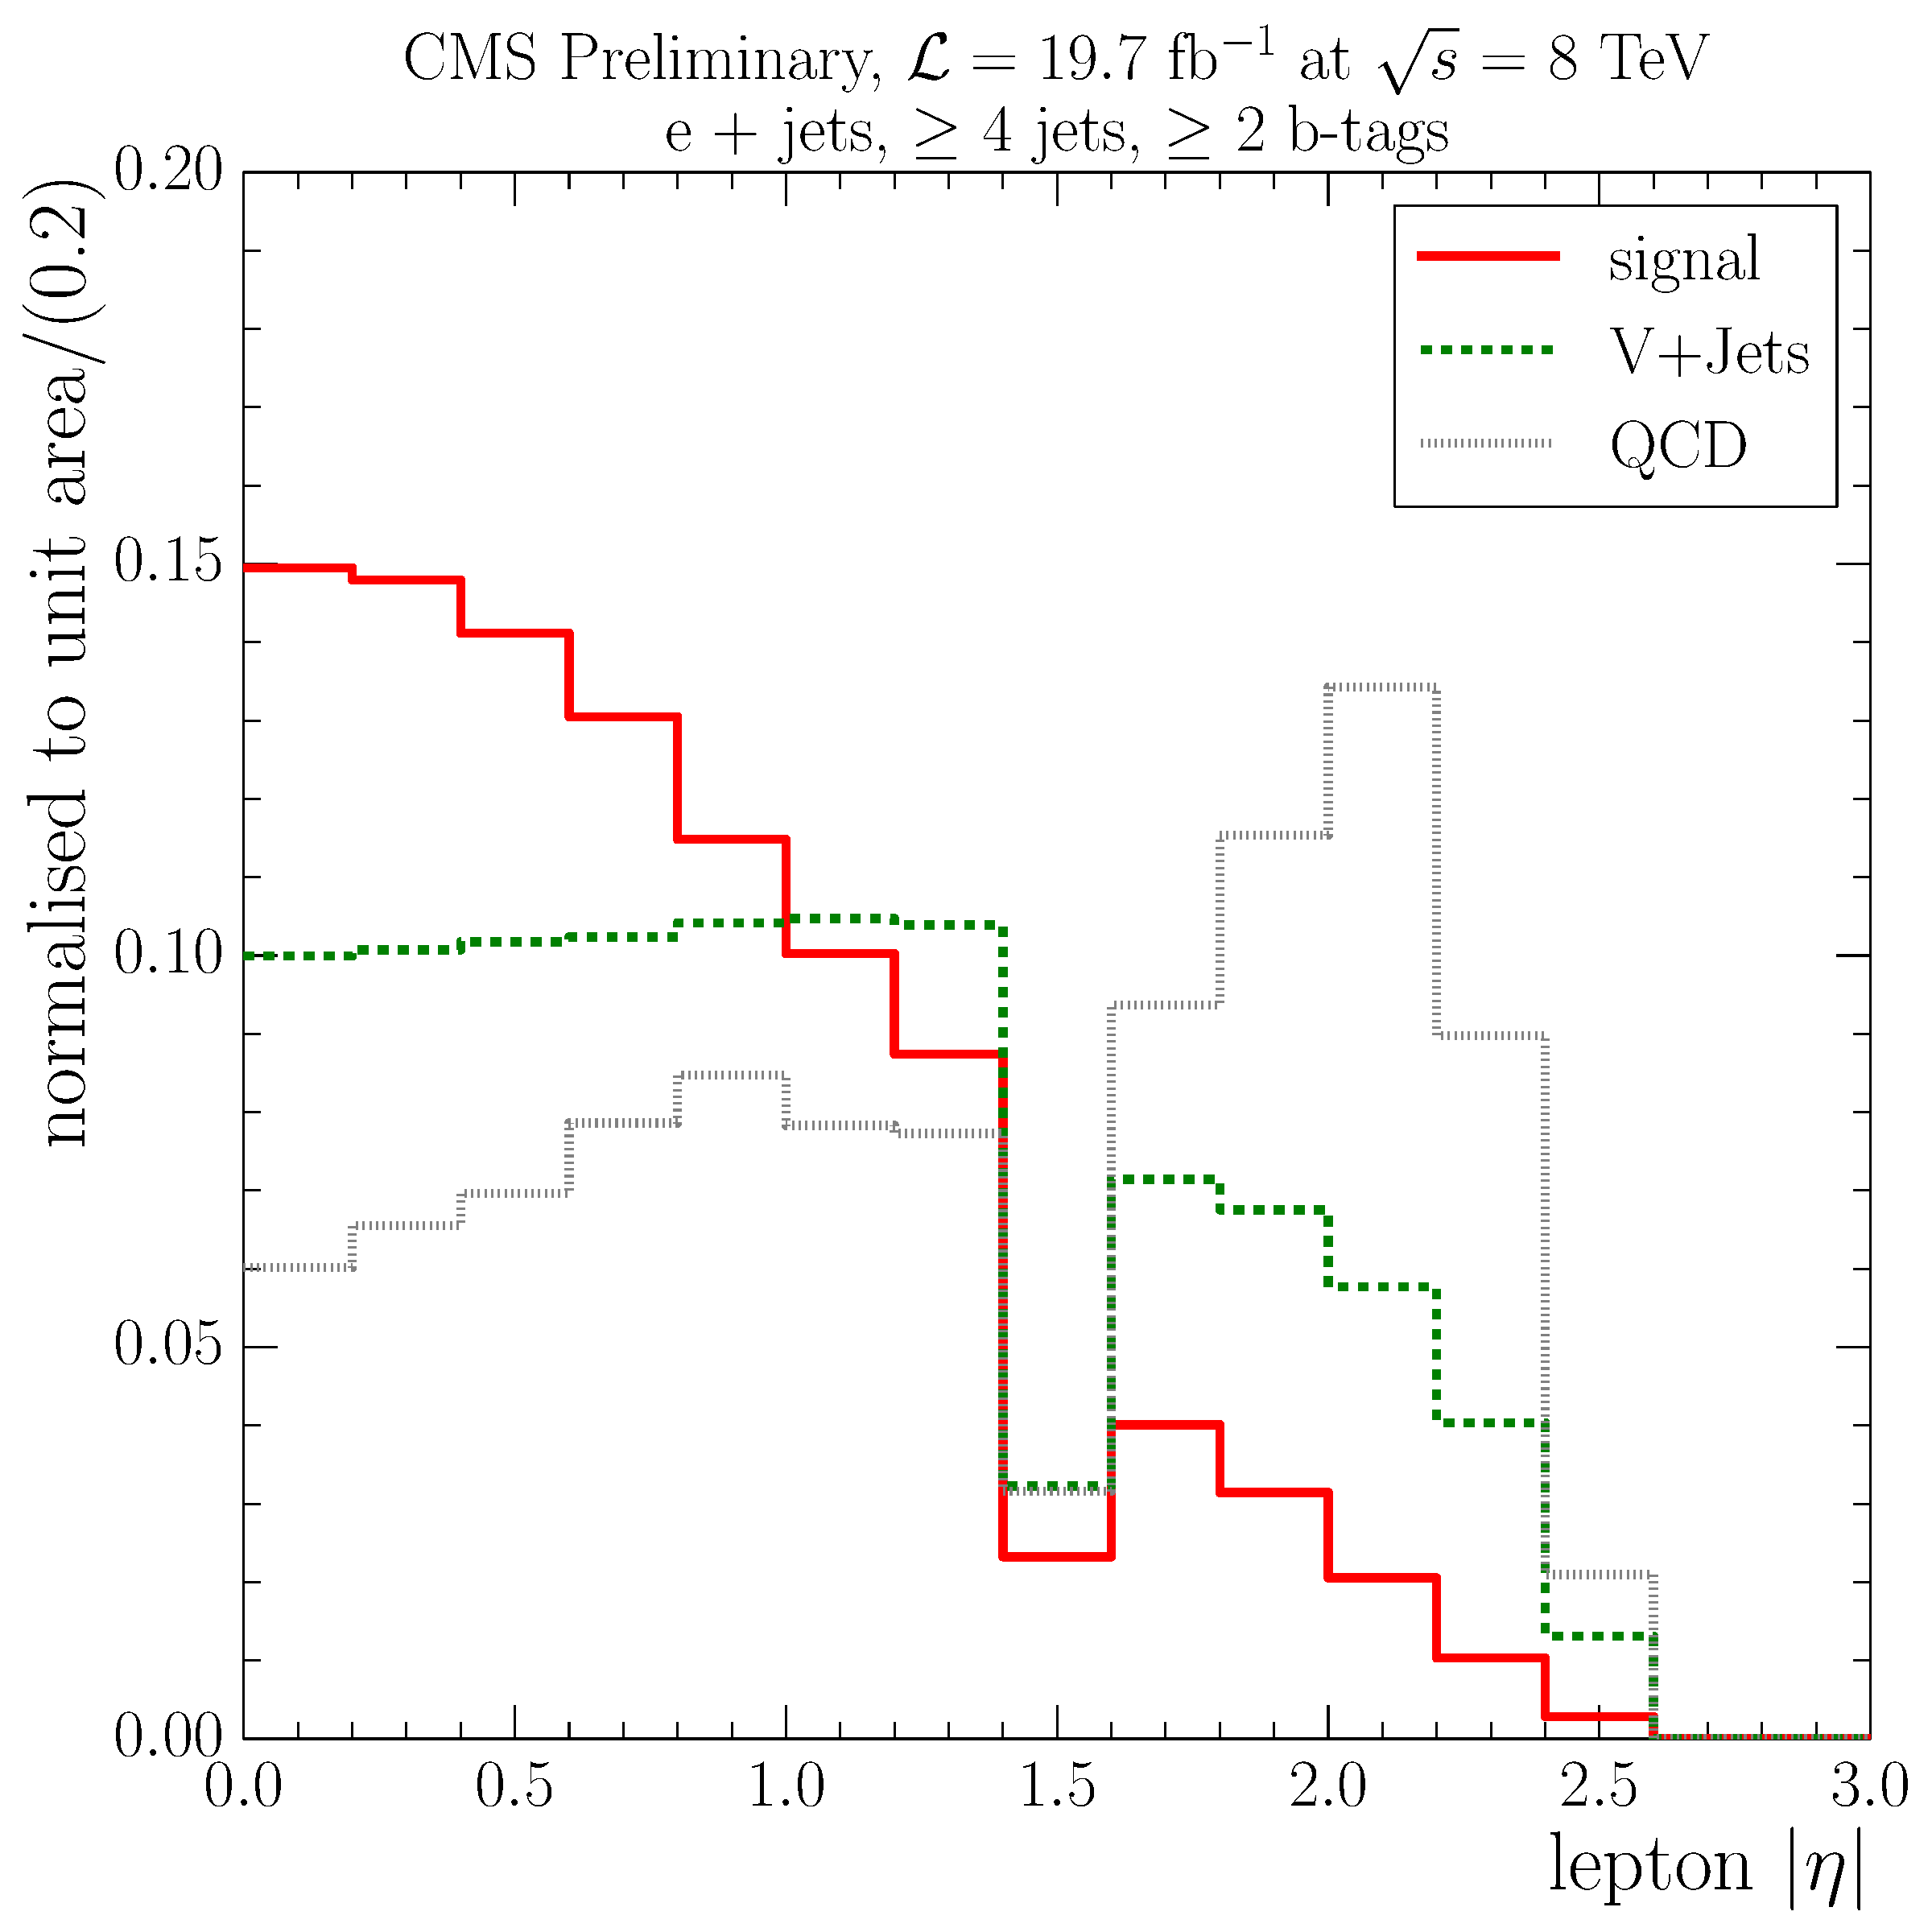
\includegraphics[width=0.3\textwidth]{measurement/HT/central/fit_templates/electron_templates_bin_0-240}}
  	{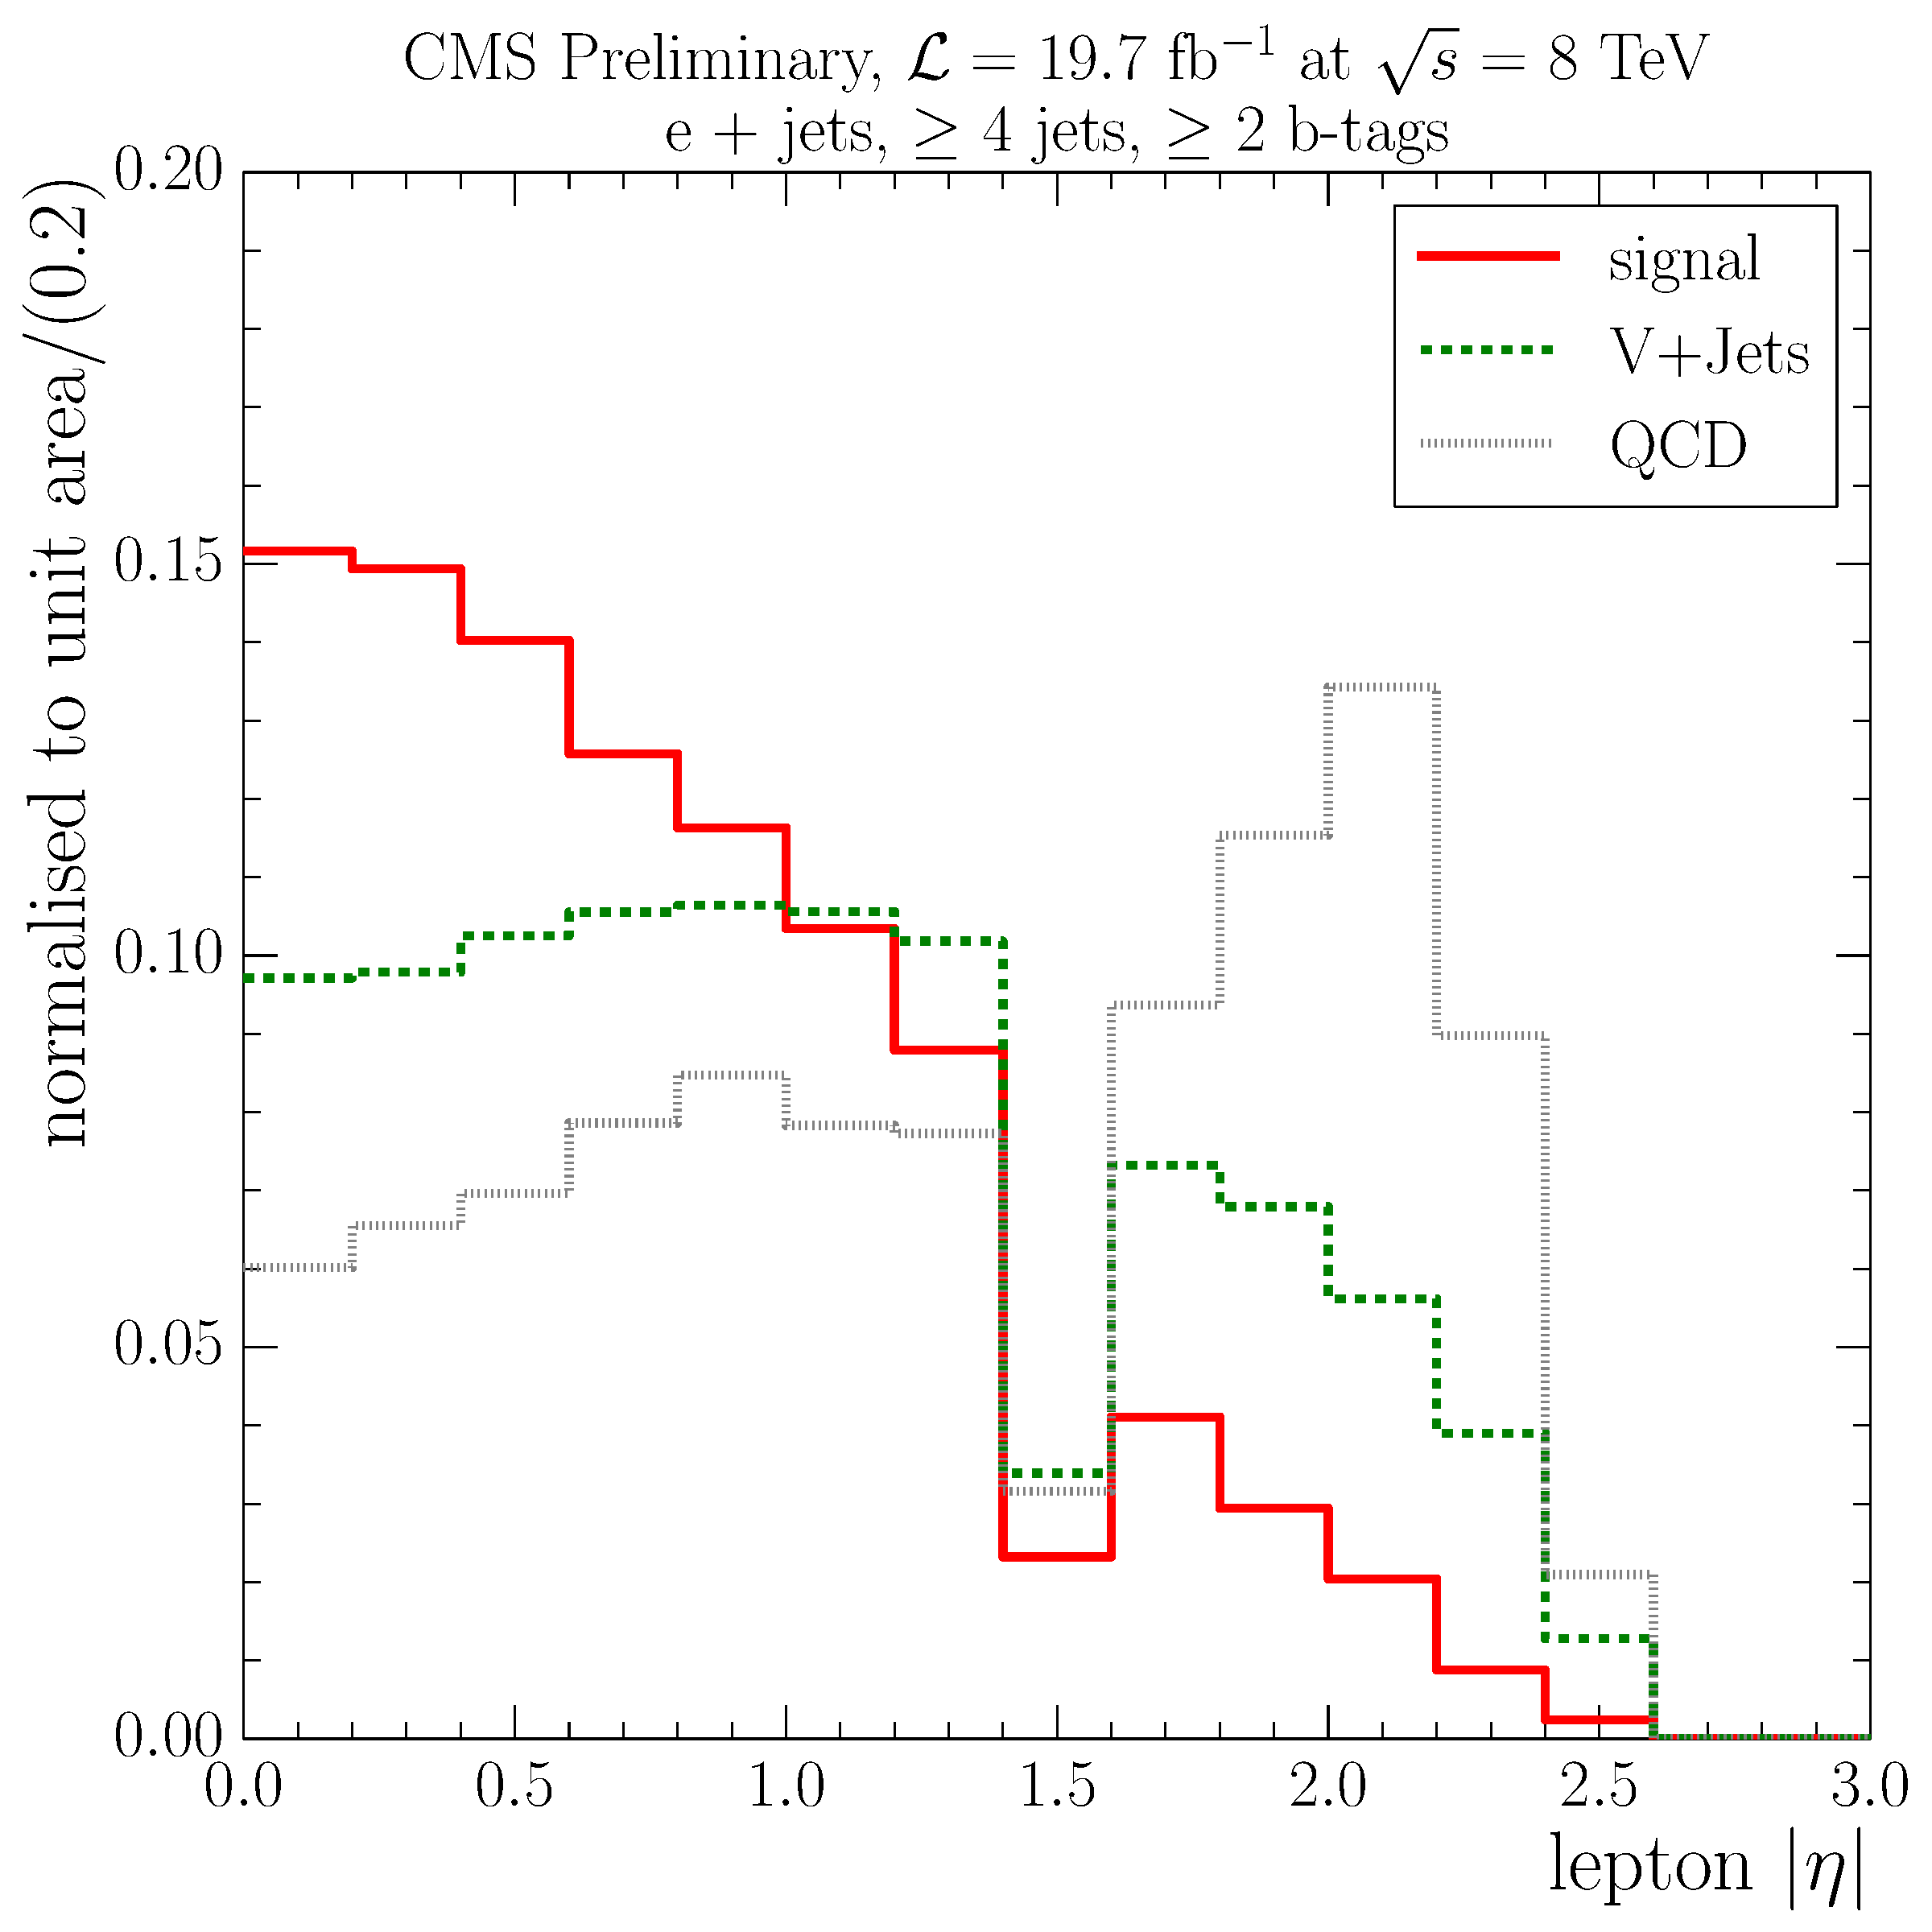
\includegraphics[width=0.3\textwidth]{measurement/HT/central/fit_templates/electron_templates_bin_240-280}}
  	{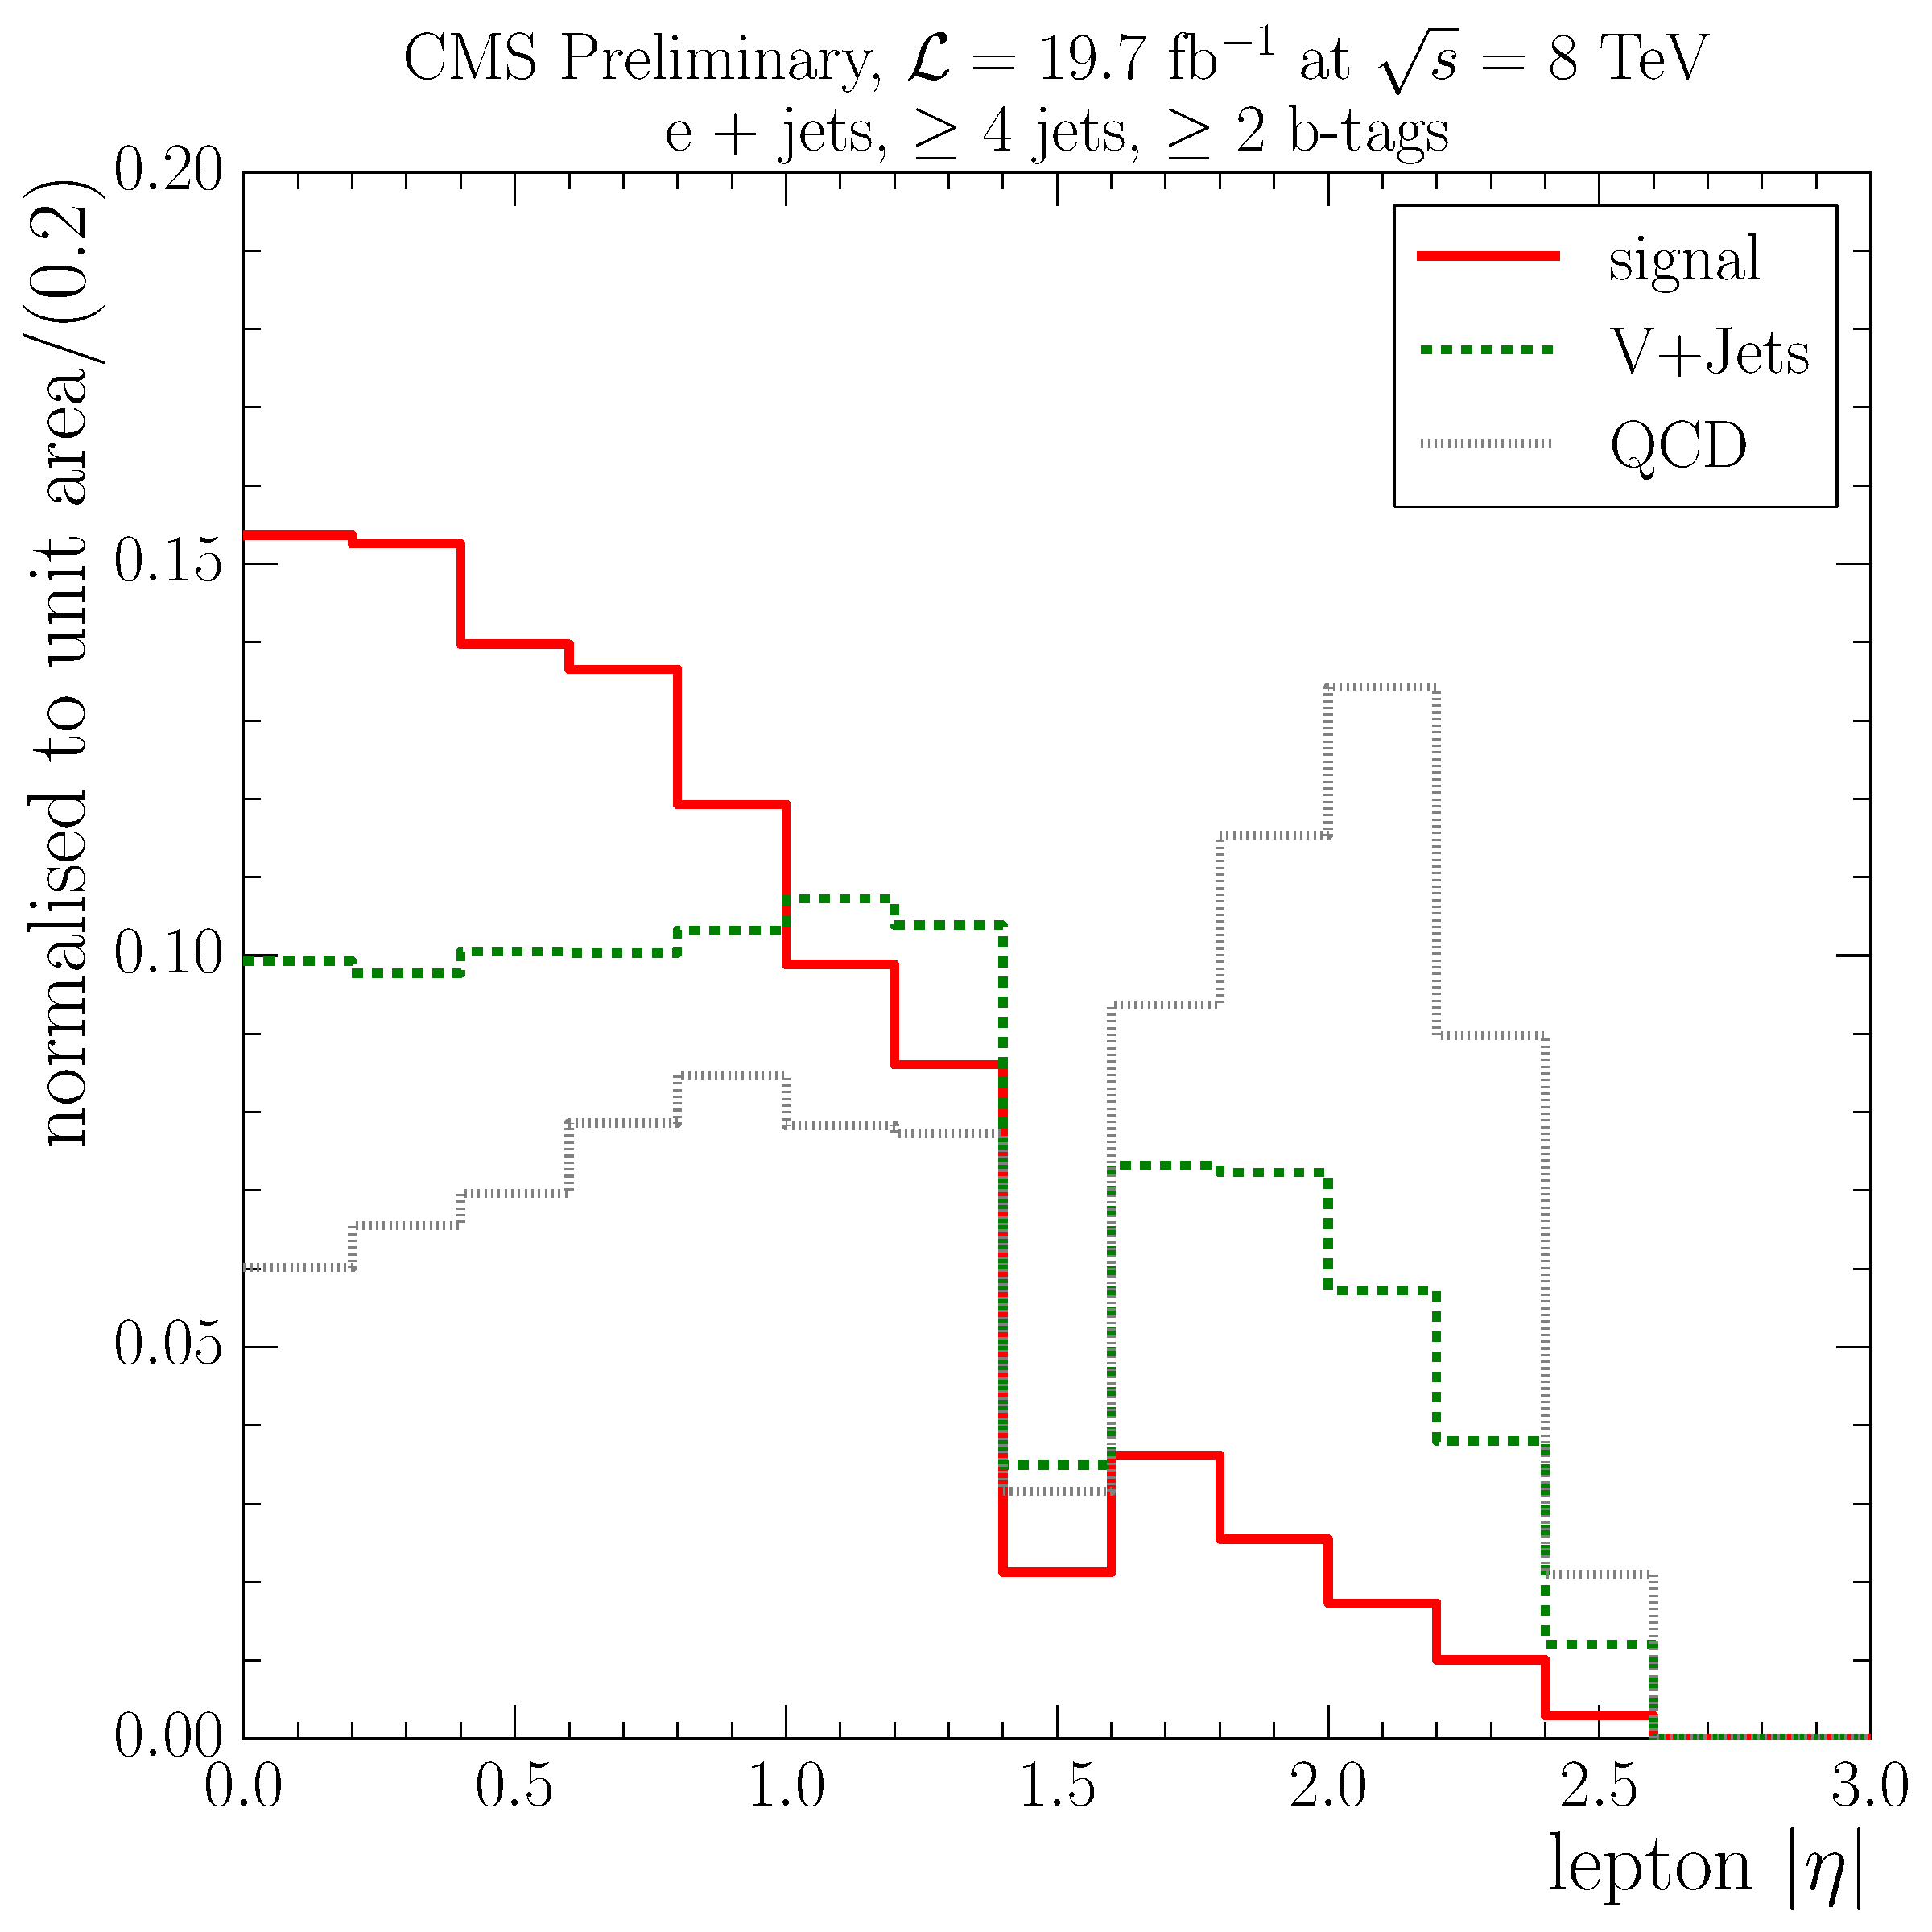
\includegraphics[width=0.3\textwidth]{measurement/HT/central/fit_templates/electron_templates_bin_280-330}}\\
  	{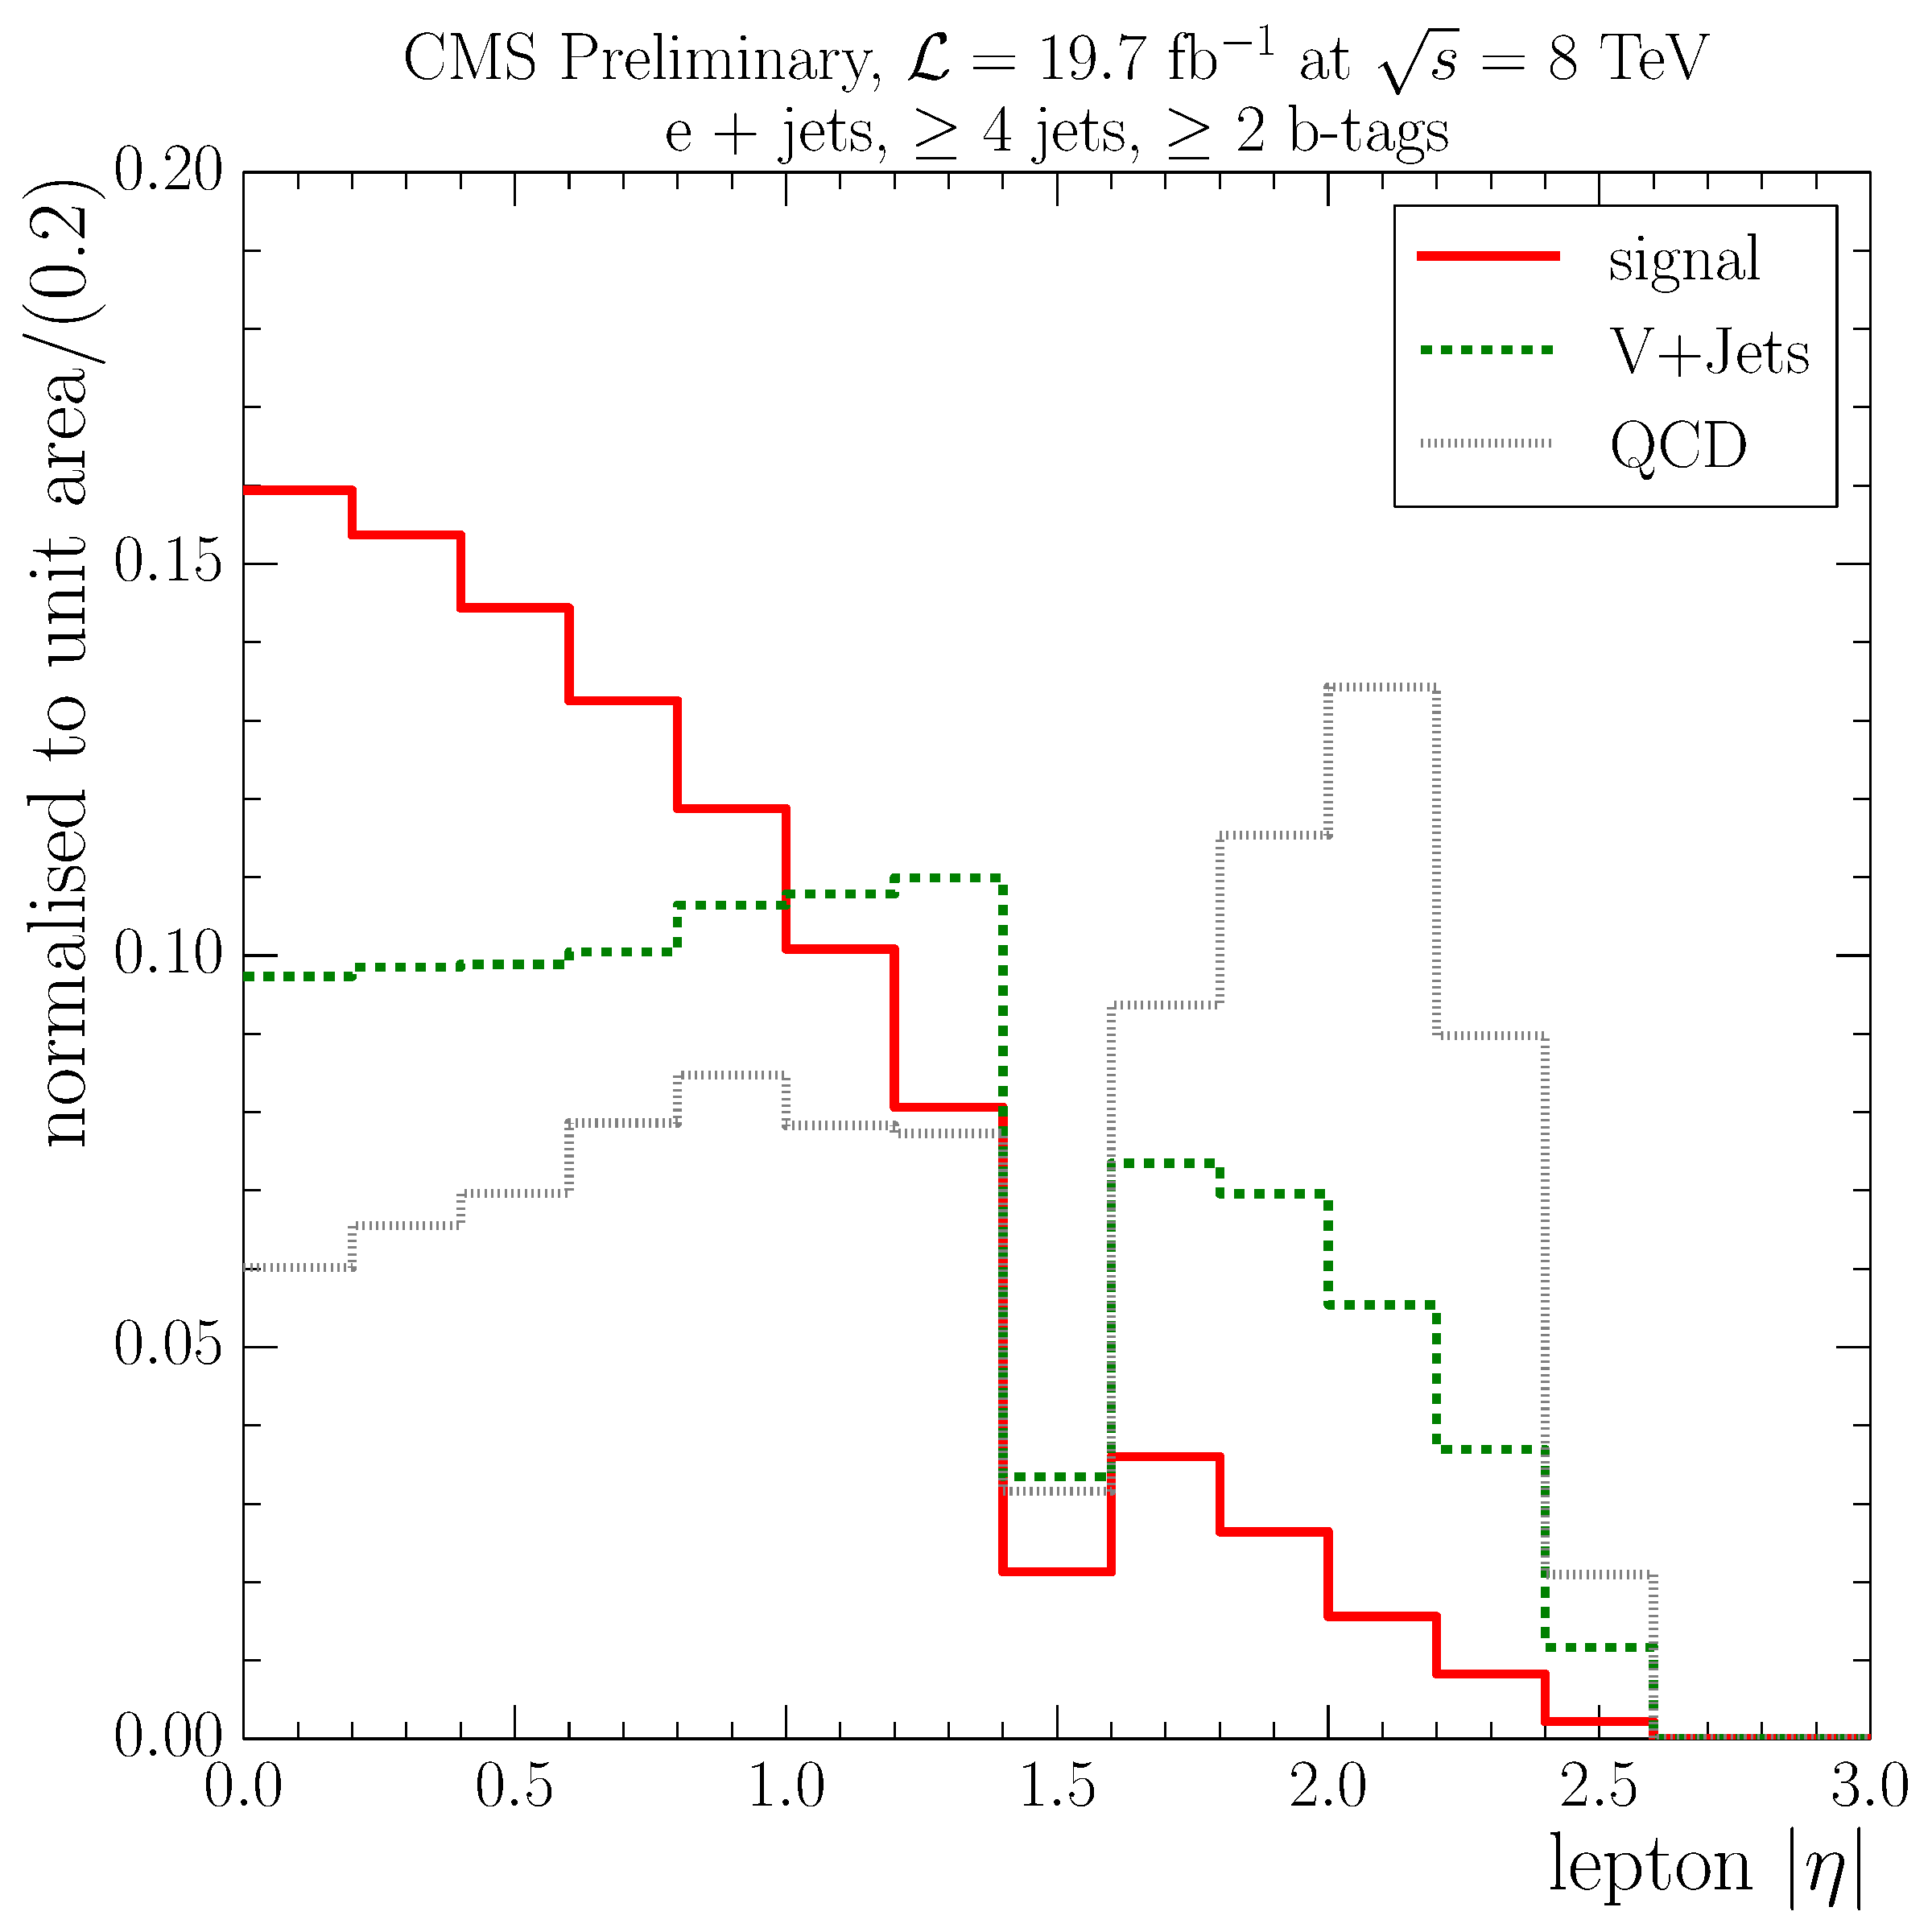
\includegraphics[width=0.3\textwidth]{measurement/HT/central/fit_templates/electron_templates_bin_330-380}}
  	{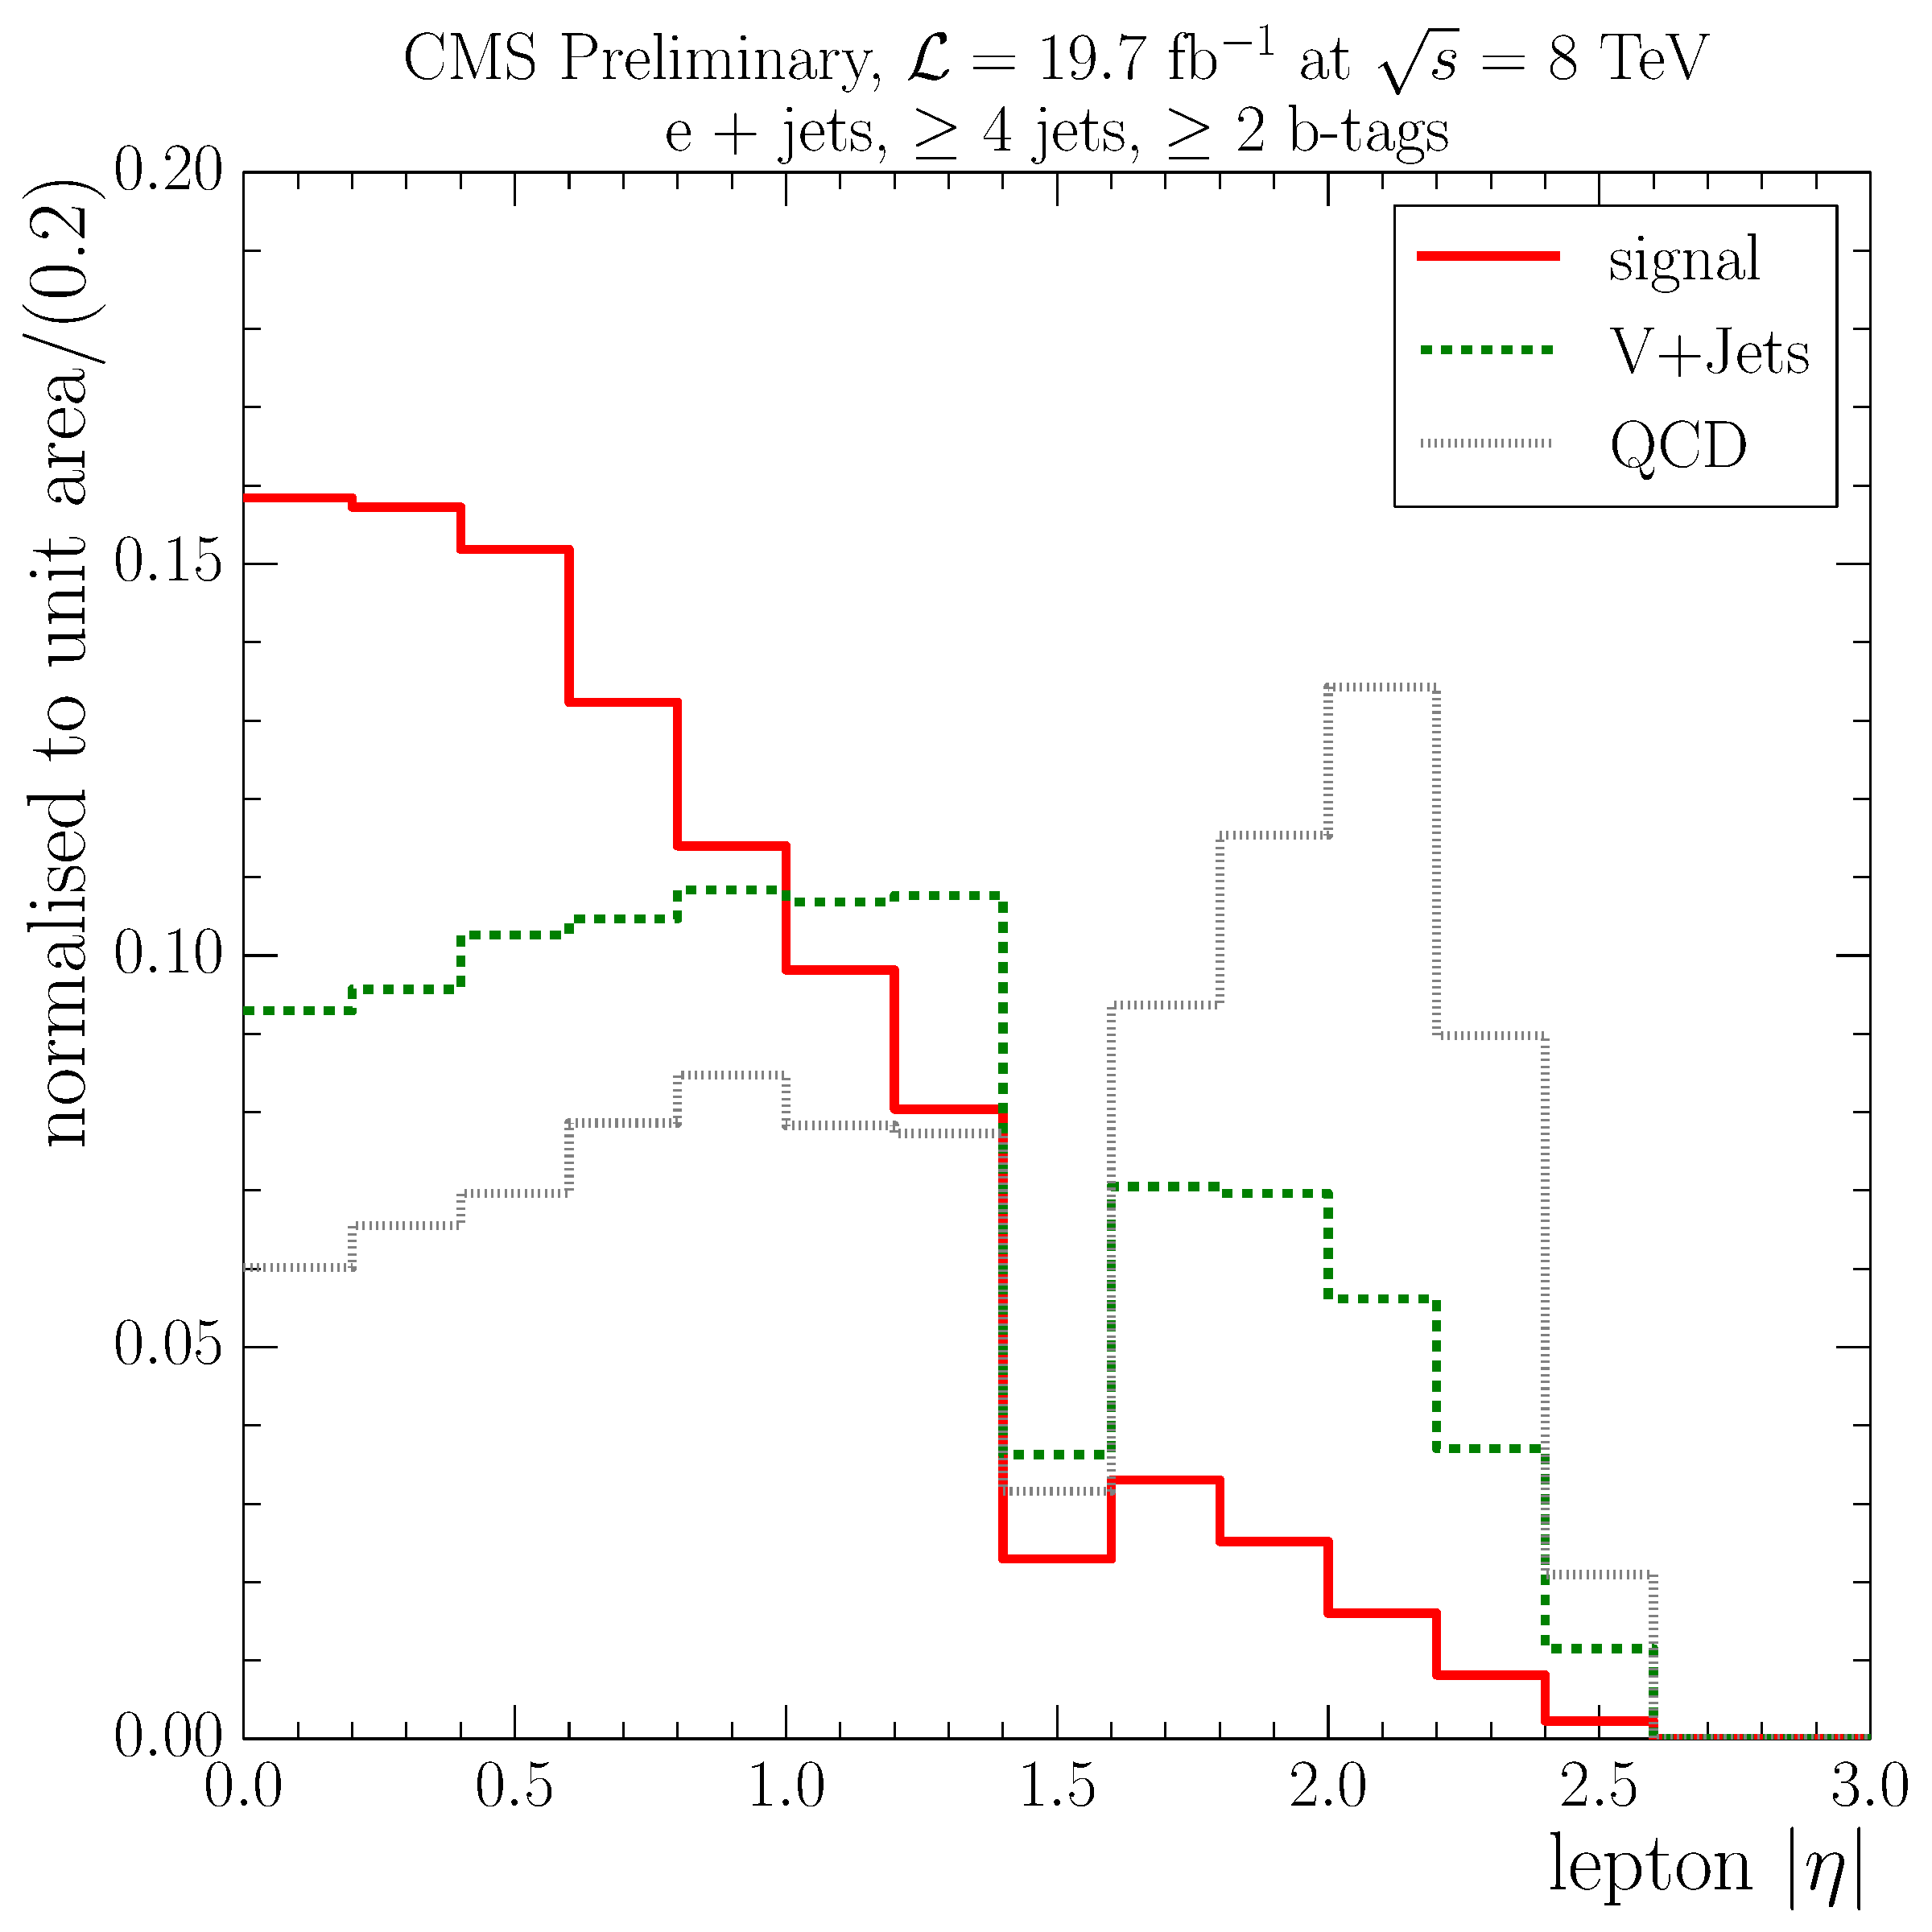
\includegraphics[width=0.3\textwidth]{measurement/HT/central/fit_templates/electron_templates_bin_380-450}}
  	{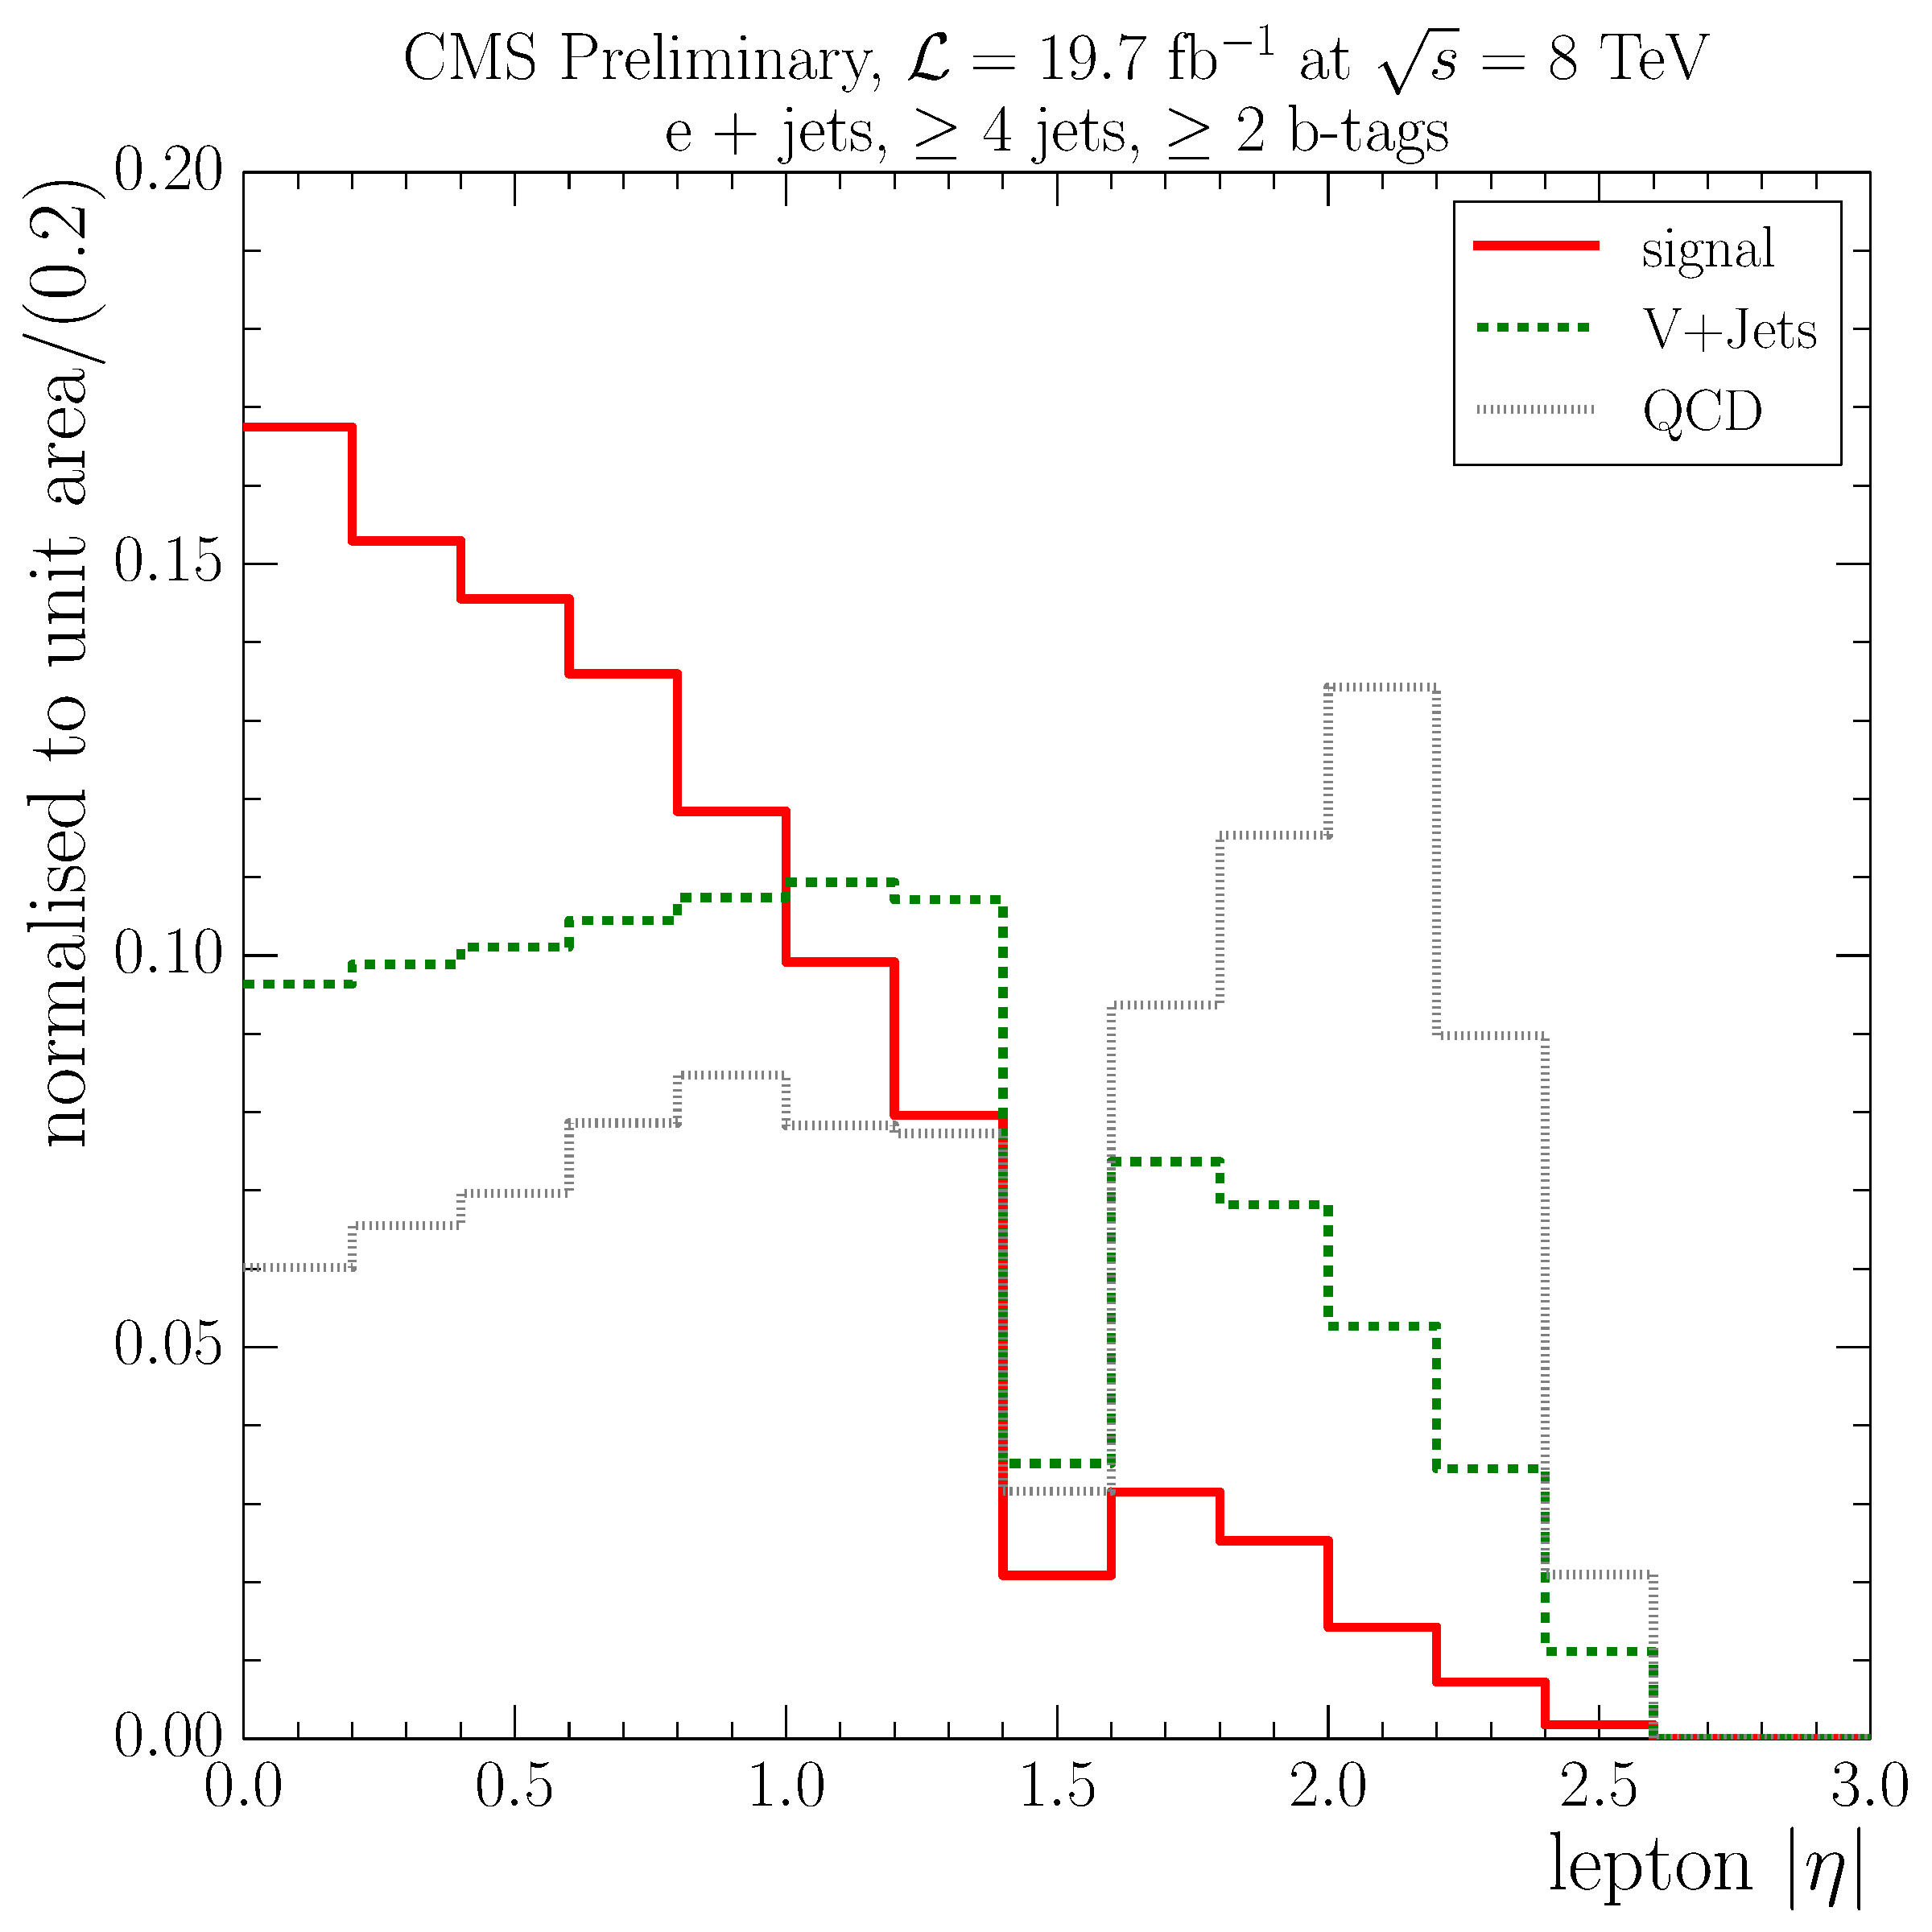
\includegraphics[width=0.3\textwidth]{measurement/HT/central/fit_templates/electron_templates_bin_450-600}}\\
  	{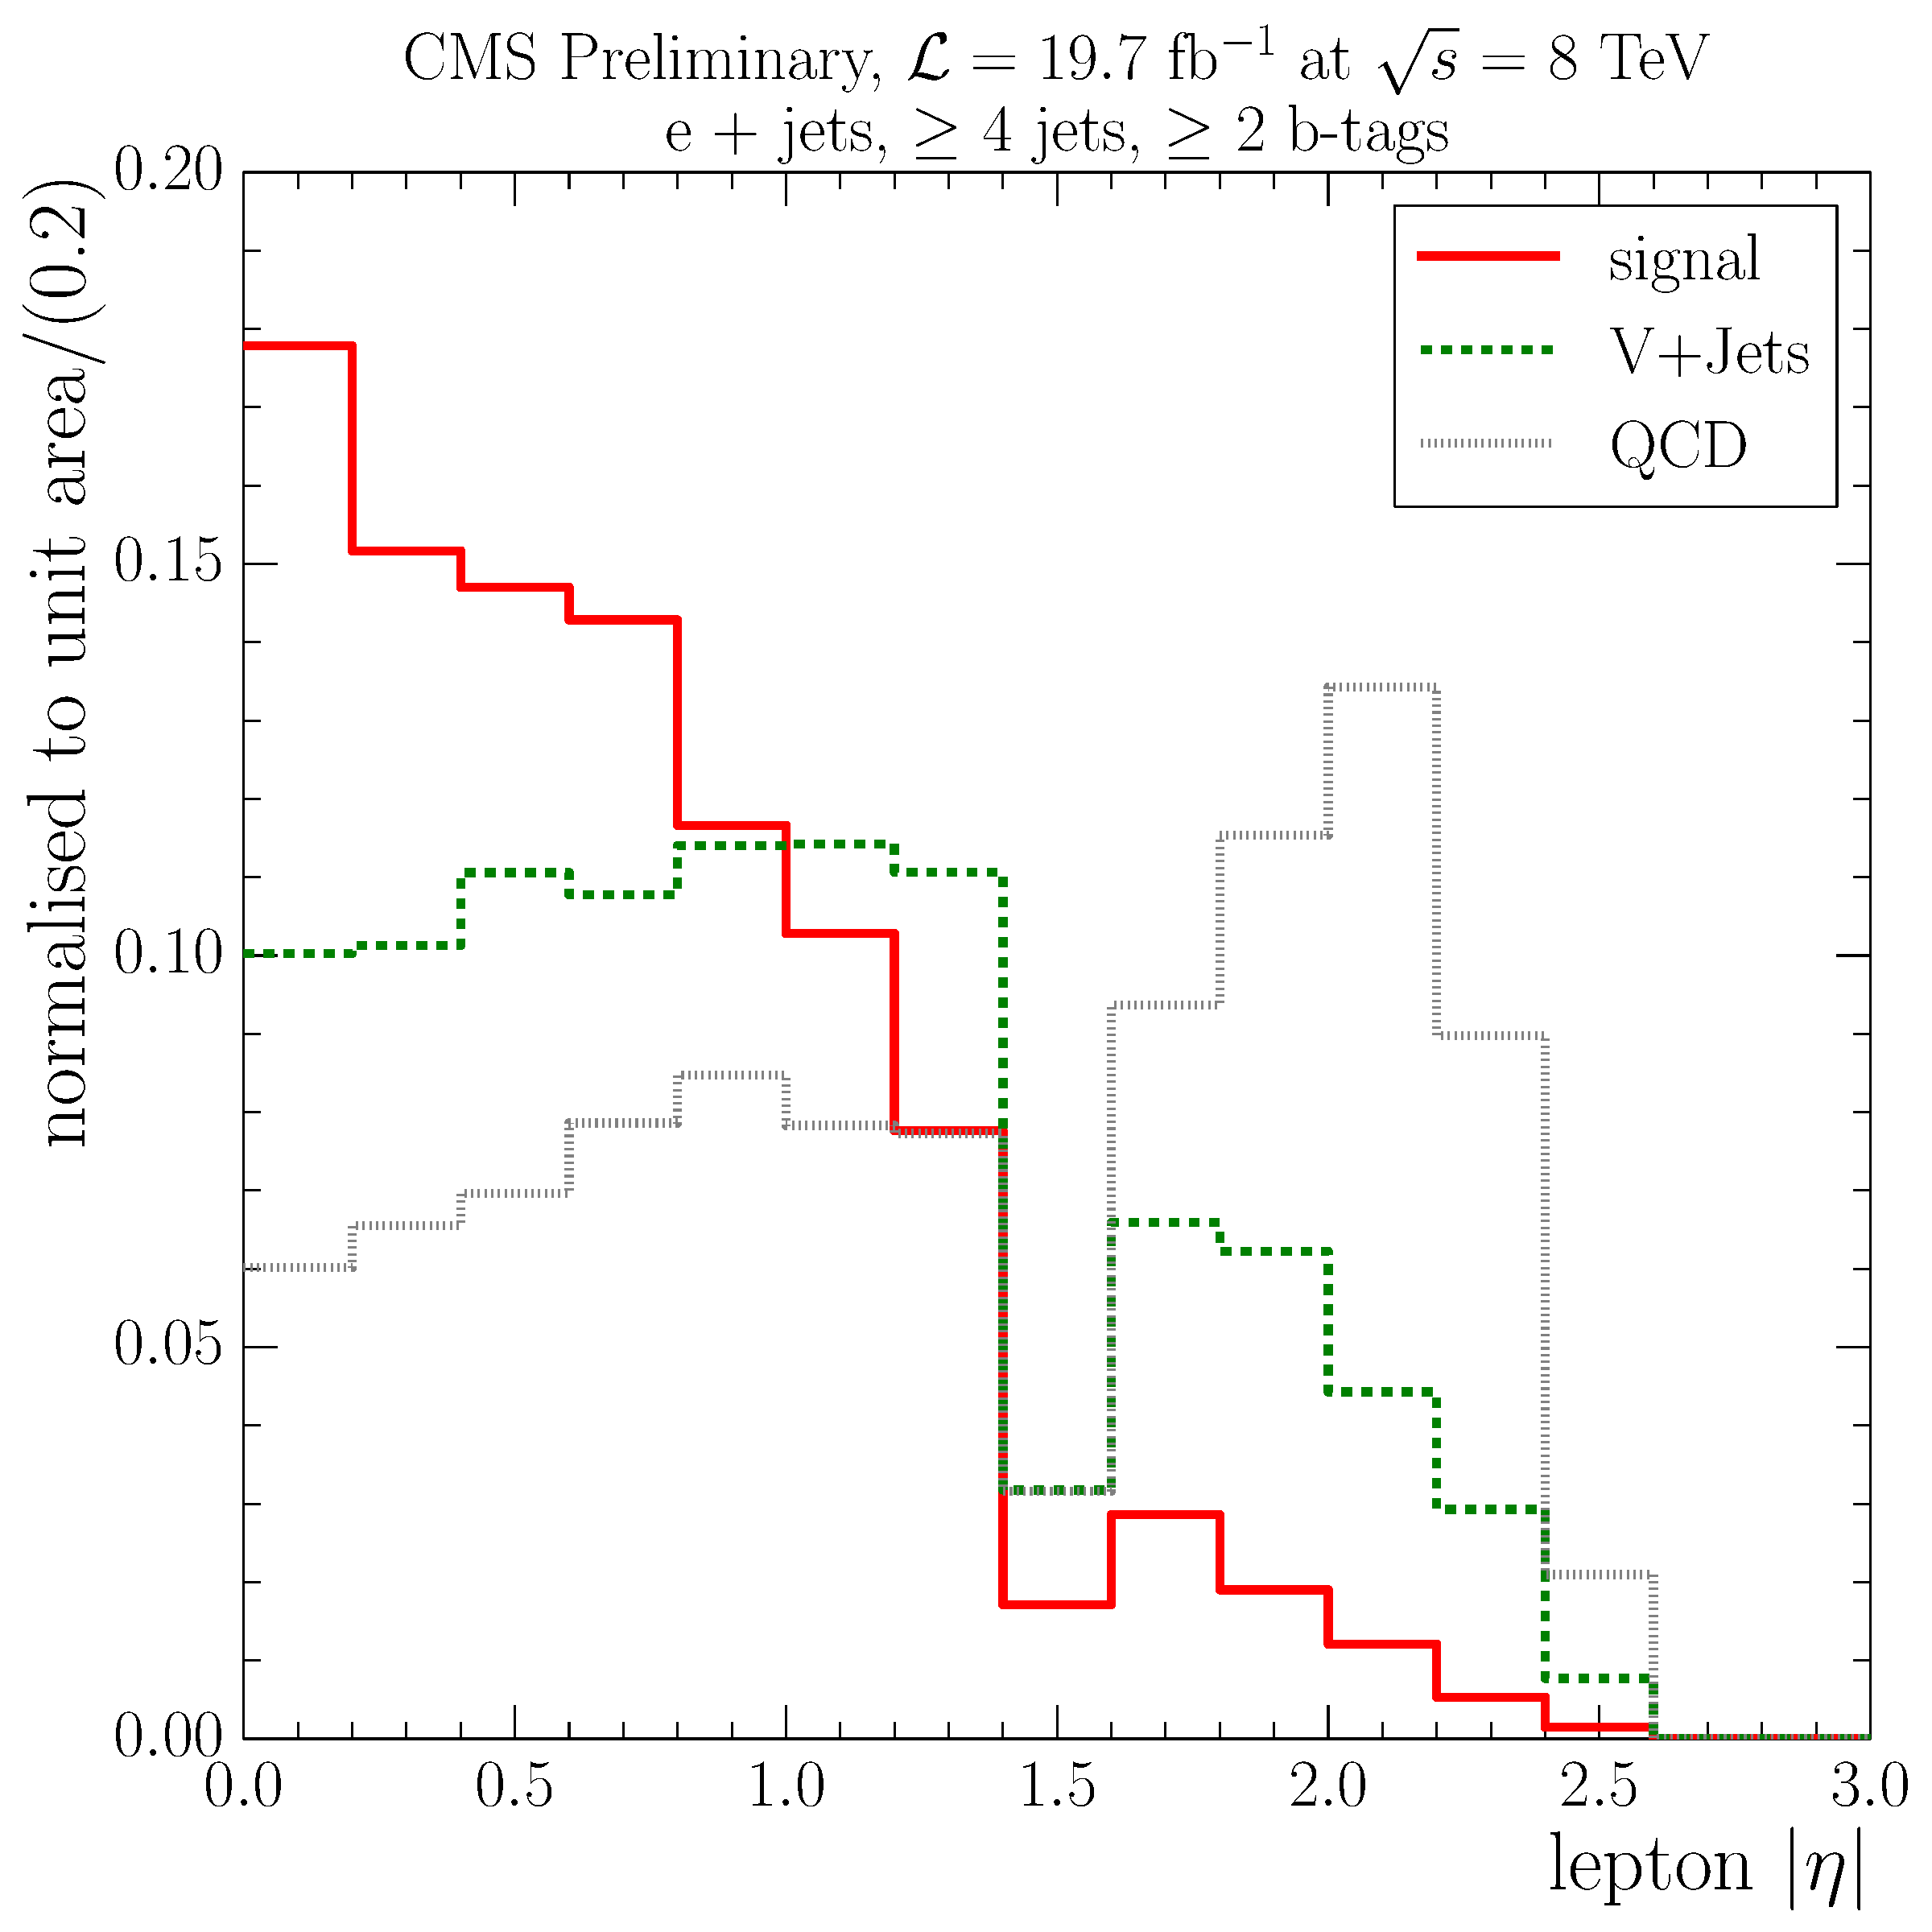
\includegraphics[width=0.3\textwidth]{measurement/HT/central/fit_templates/electron_templates_bin_600-inf}}
    \caption[Electron $\abs \eta$ templates for the fit in different bins of \HT]{Electron $\abs \eta$ templates for the
    fit in different bins of \HT, from top left to bottom: \SIrange{0}{240}{\GeV}, \SIrange{240}{280}{\GeV},
    \SIrange{280}{330}{\GeV}, \SIrange{330}{380}{\GeV}, \SIrange{380}{450}{\GeV}, \SIrange{450}{600}{\GeV} and $\geq
    \SI{600}{\GeV}$.}
    \label{fig:fit_tempaltes_HT_electron}
\end{figure}

\begin{figure}[!htbp]
	\centering
  	{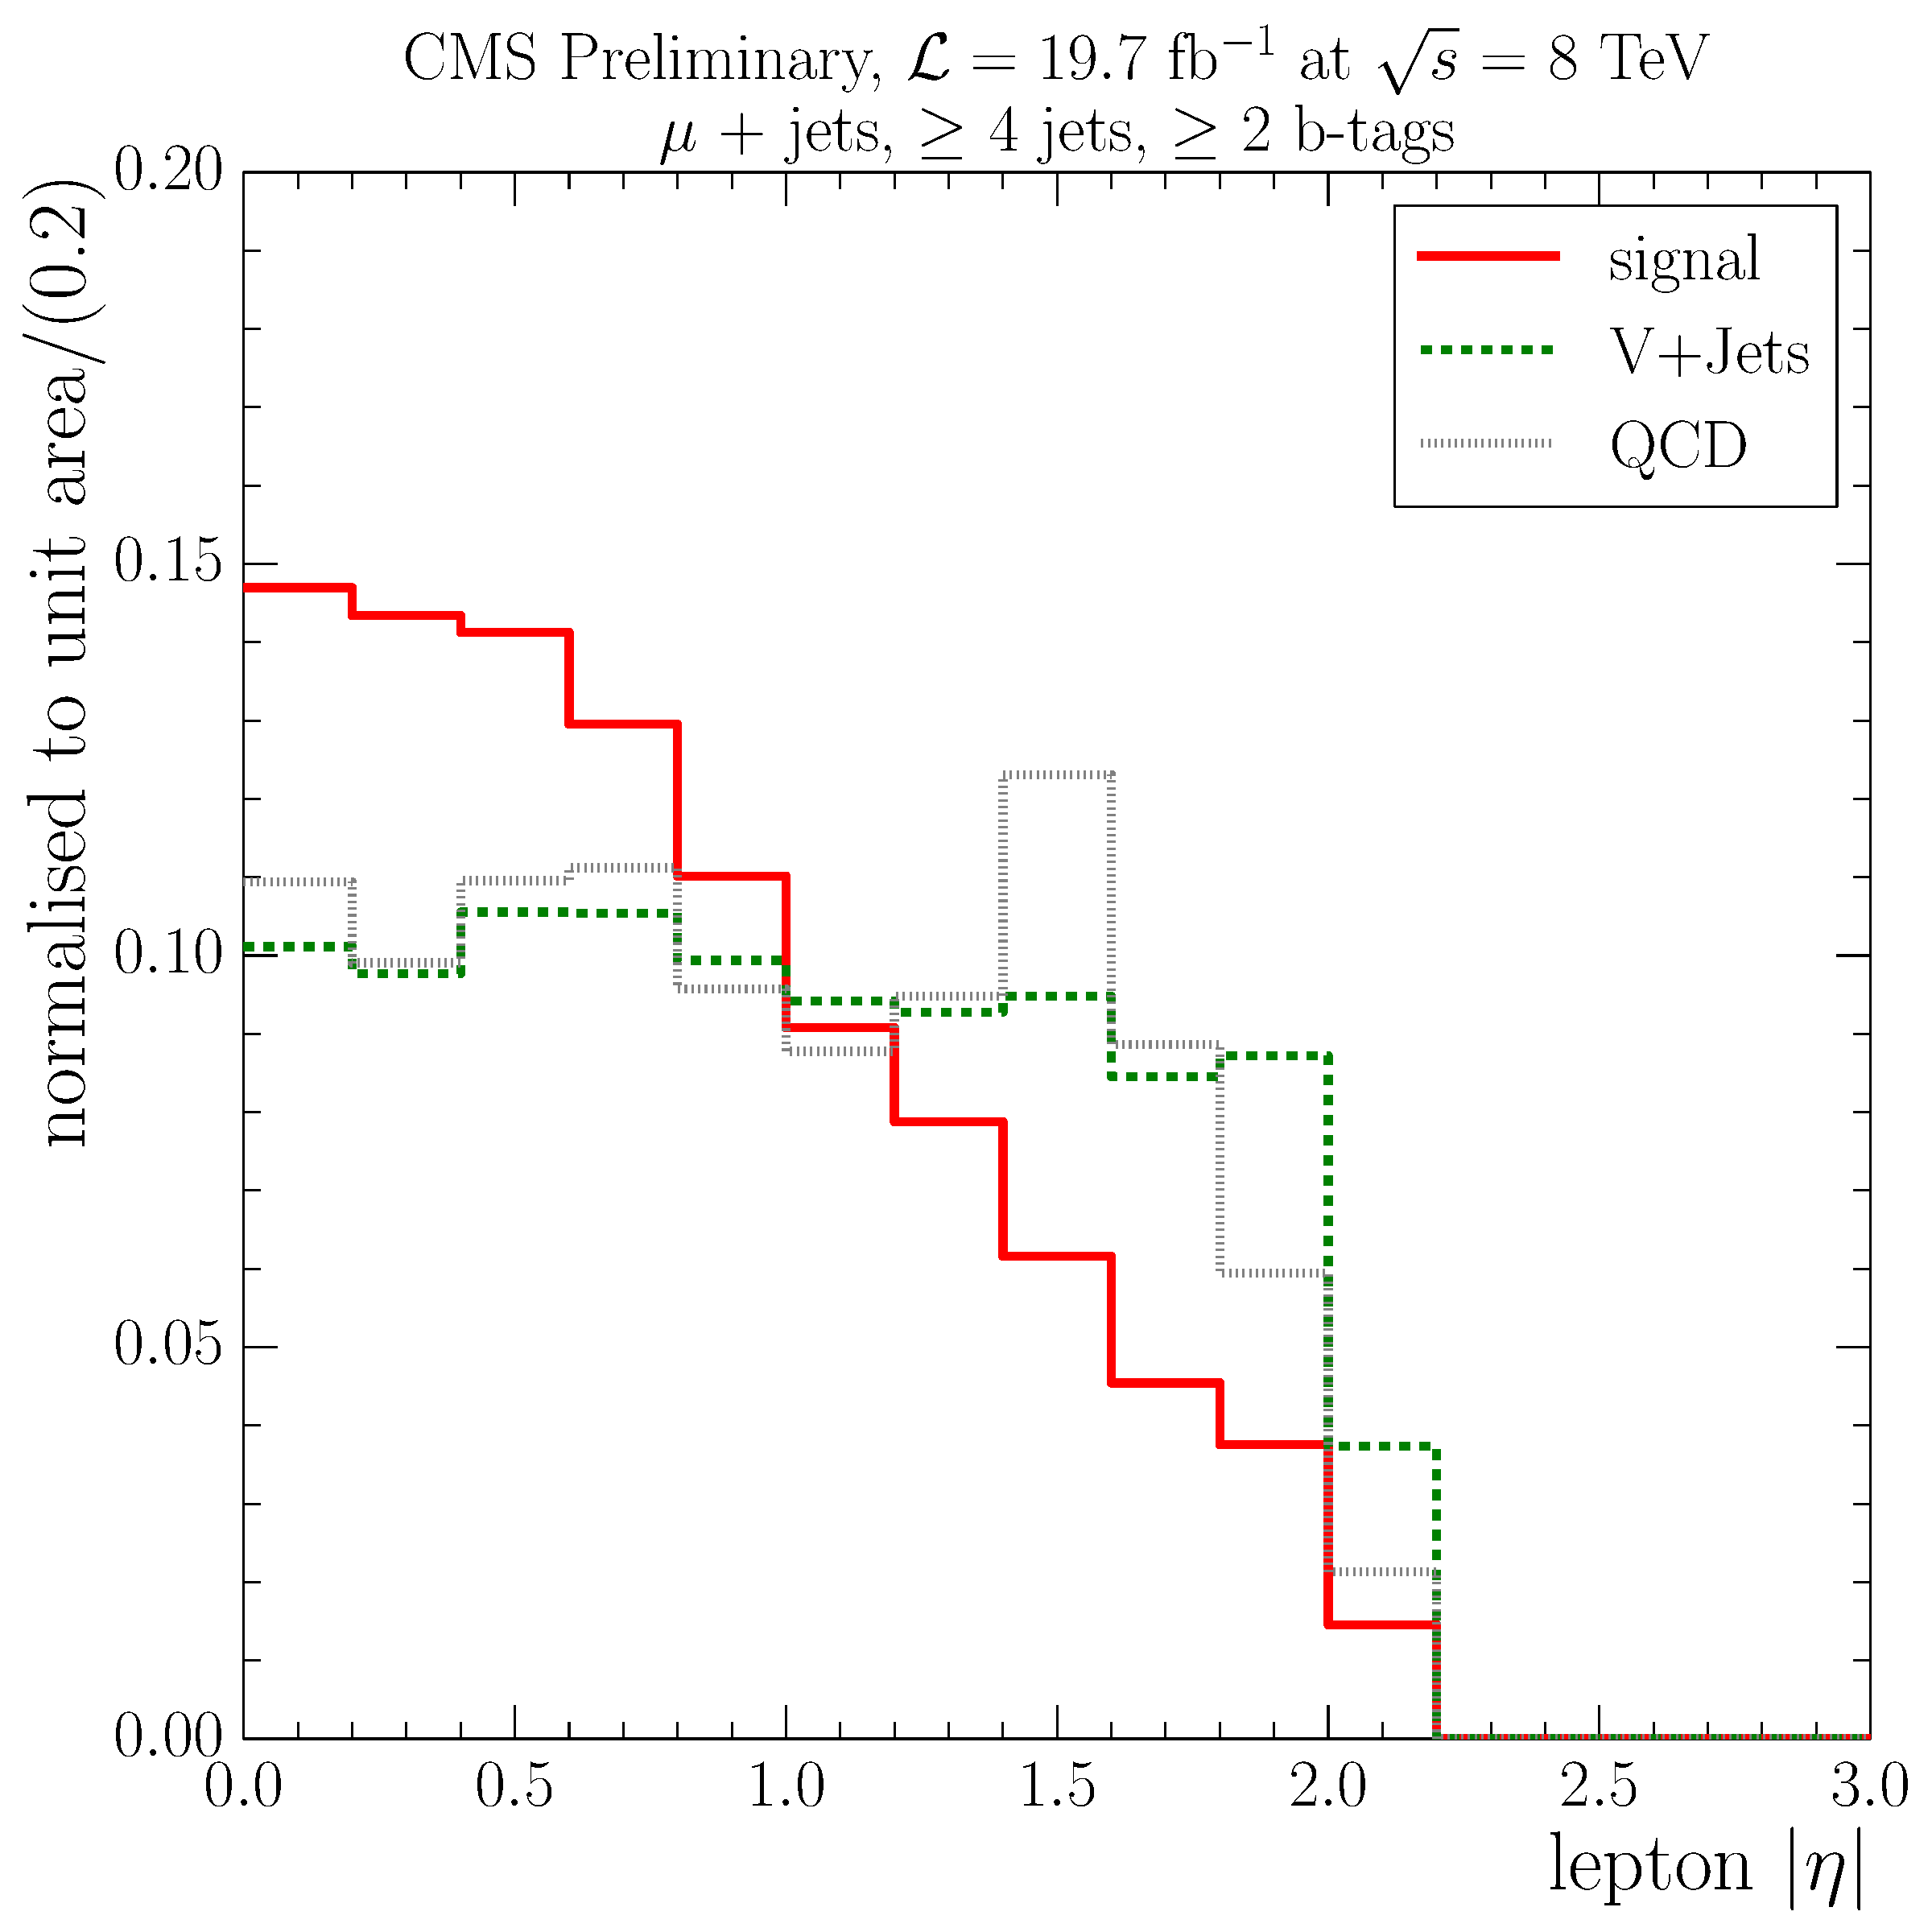
\includegraphics[width=0.3\textwidth]{measurement/HT/central/fit_templates/muon_templates_bin_0-240}}
  	{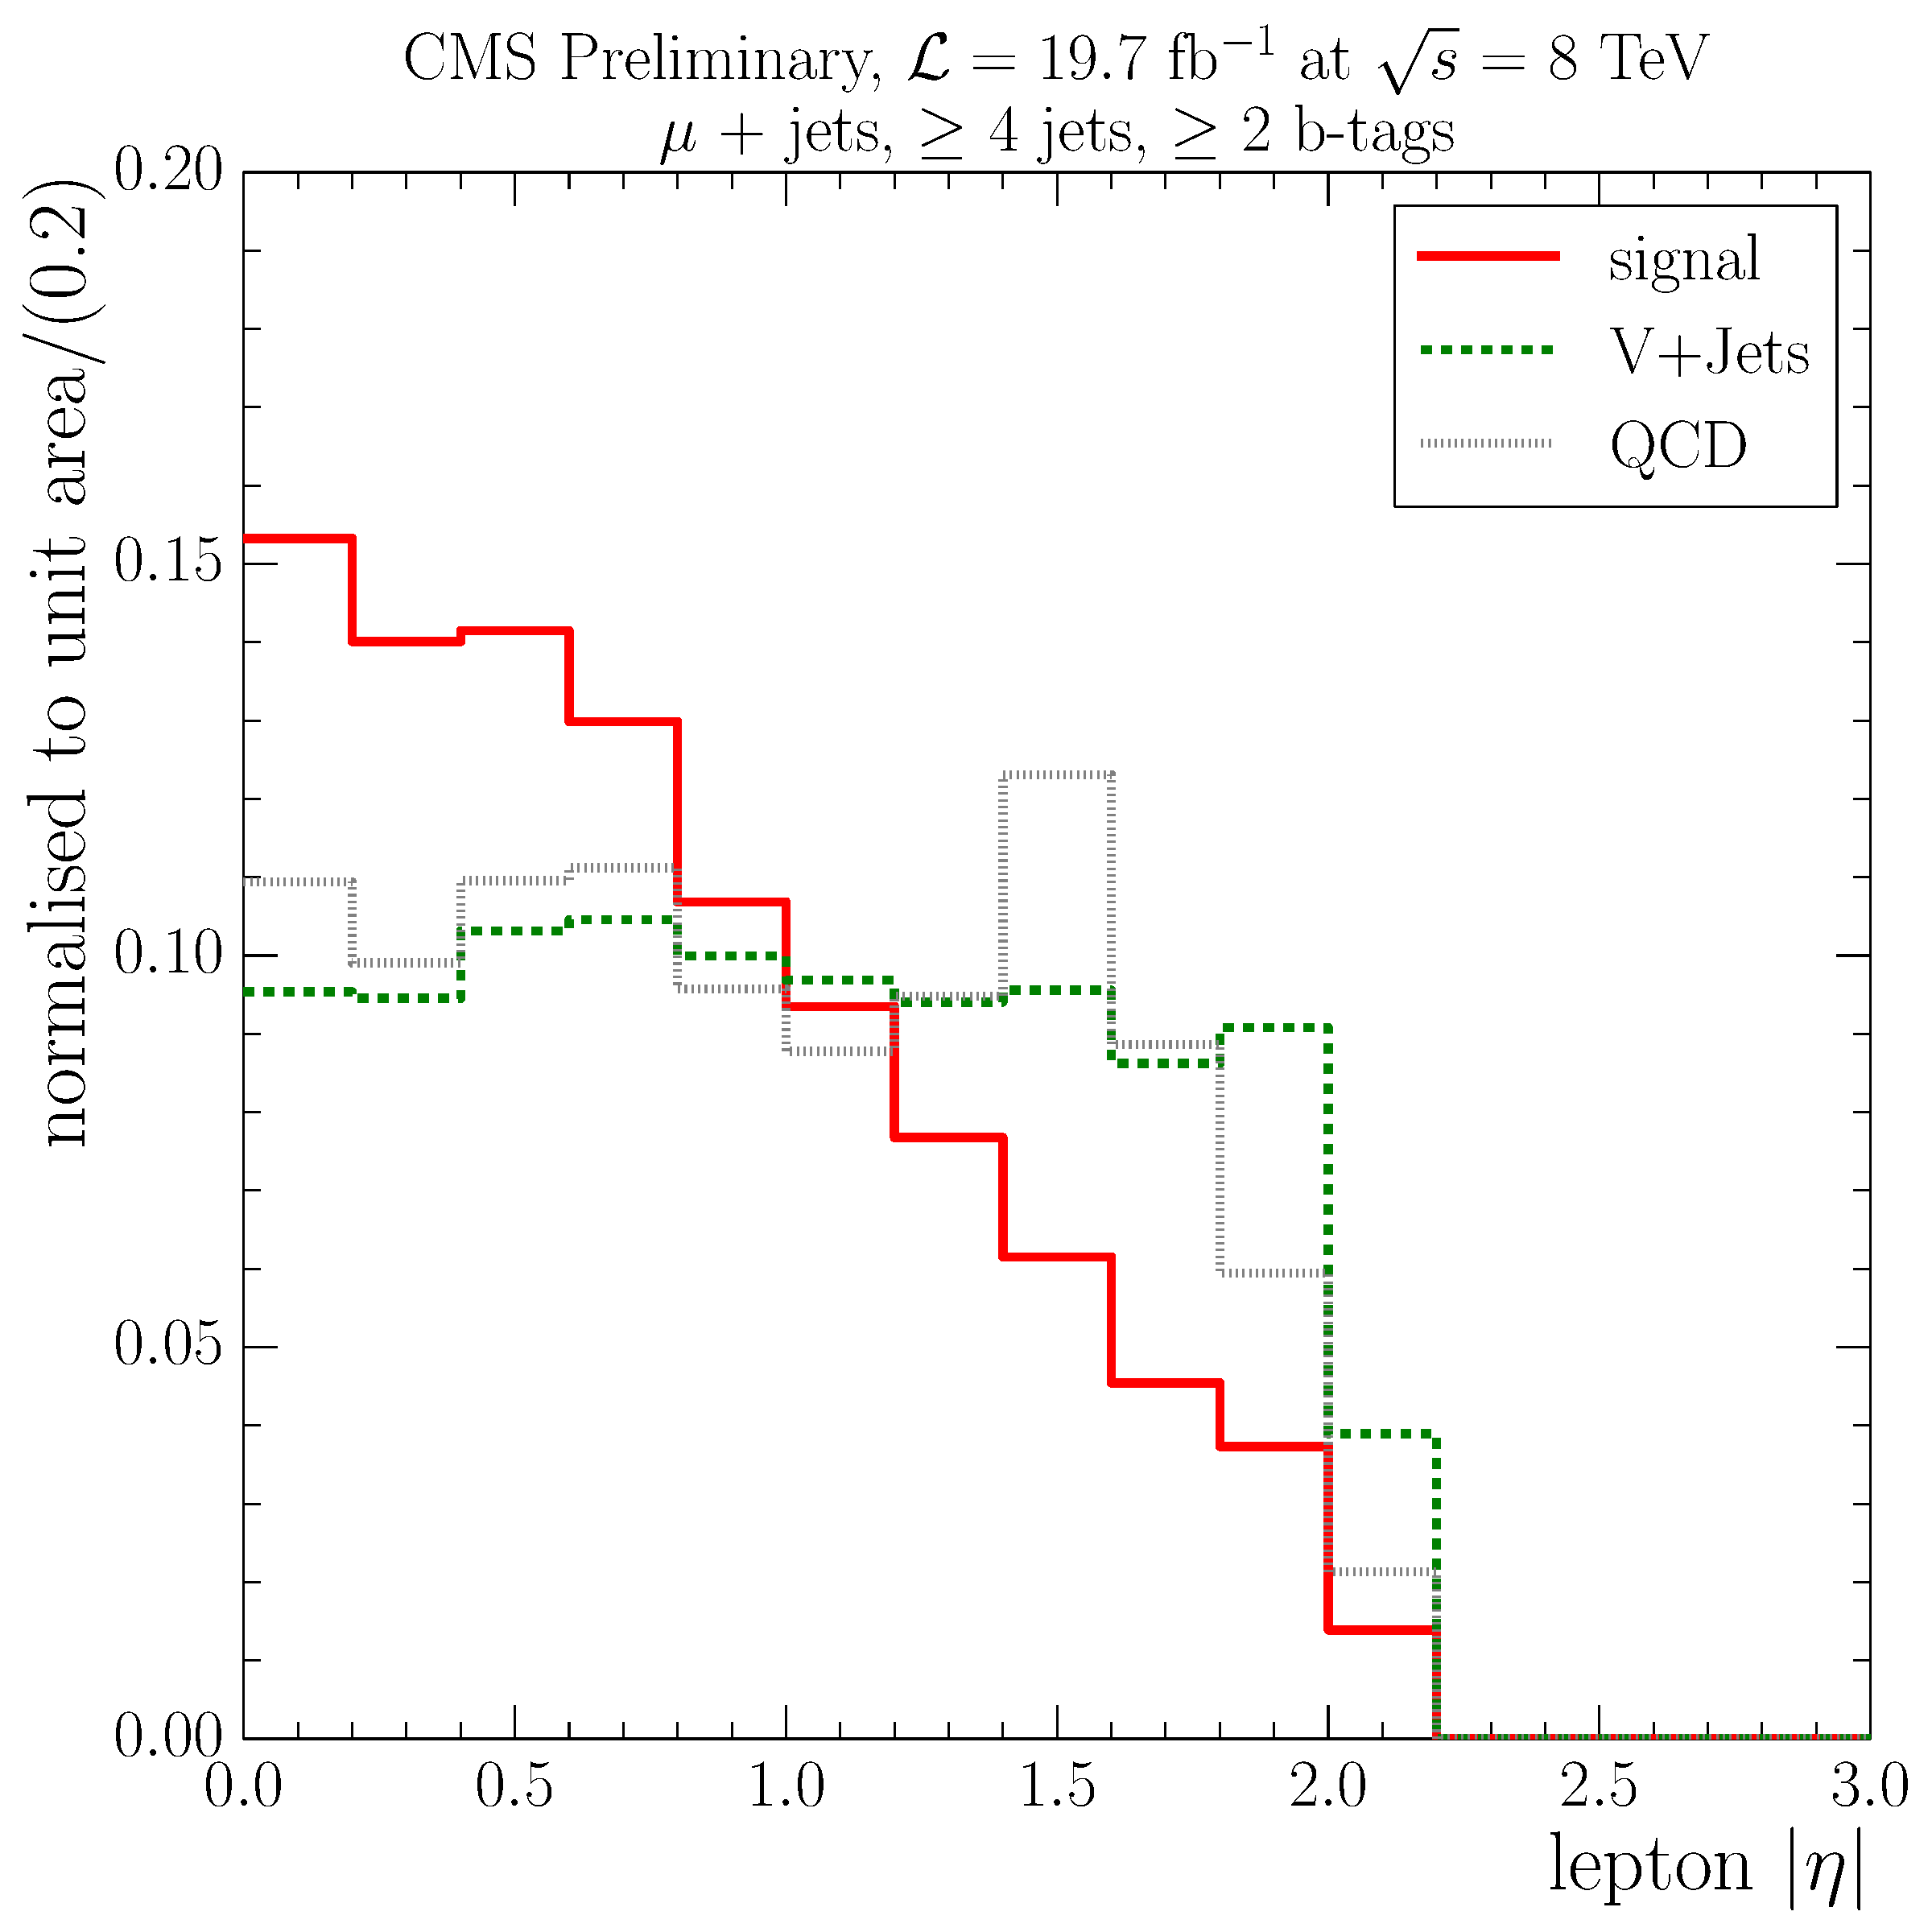
\includegraphics[width=0.3\textwidth]{measurement/HT/central/fit_templates/muon_templates_bin_240-280}}
  	{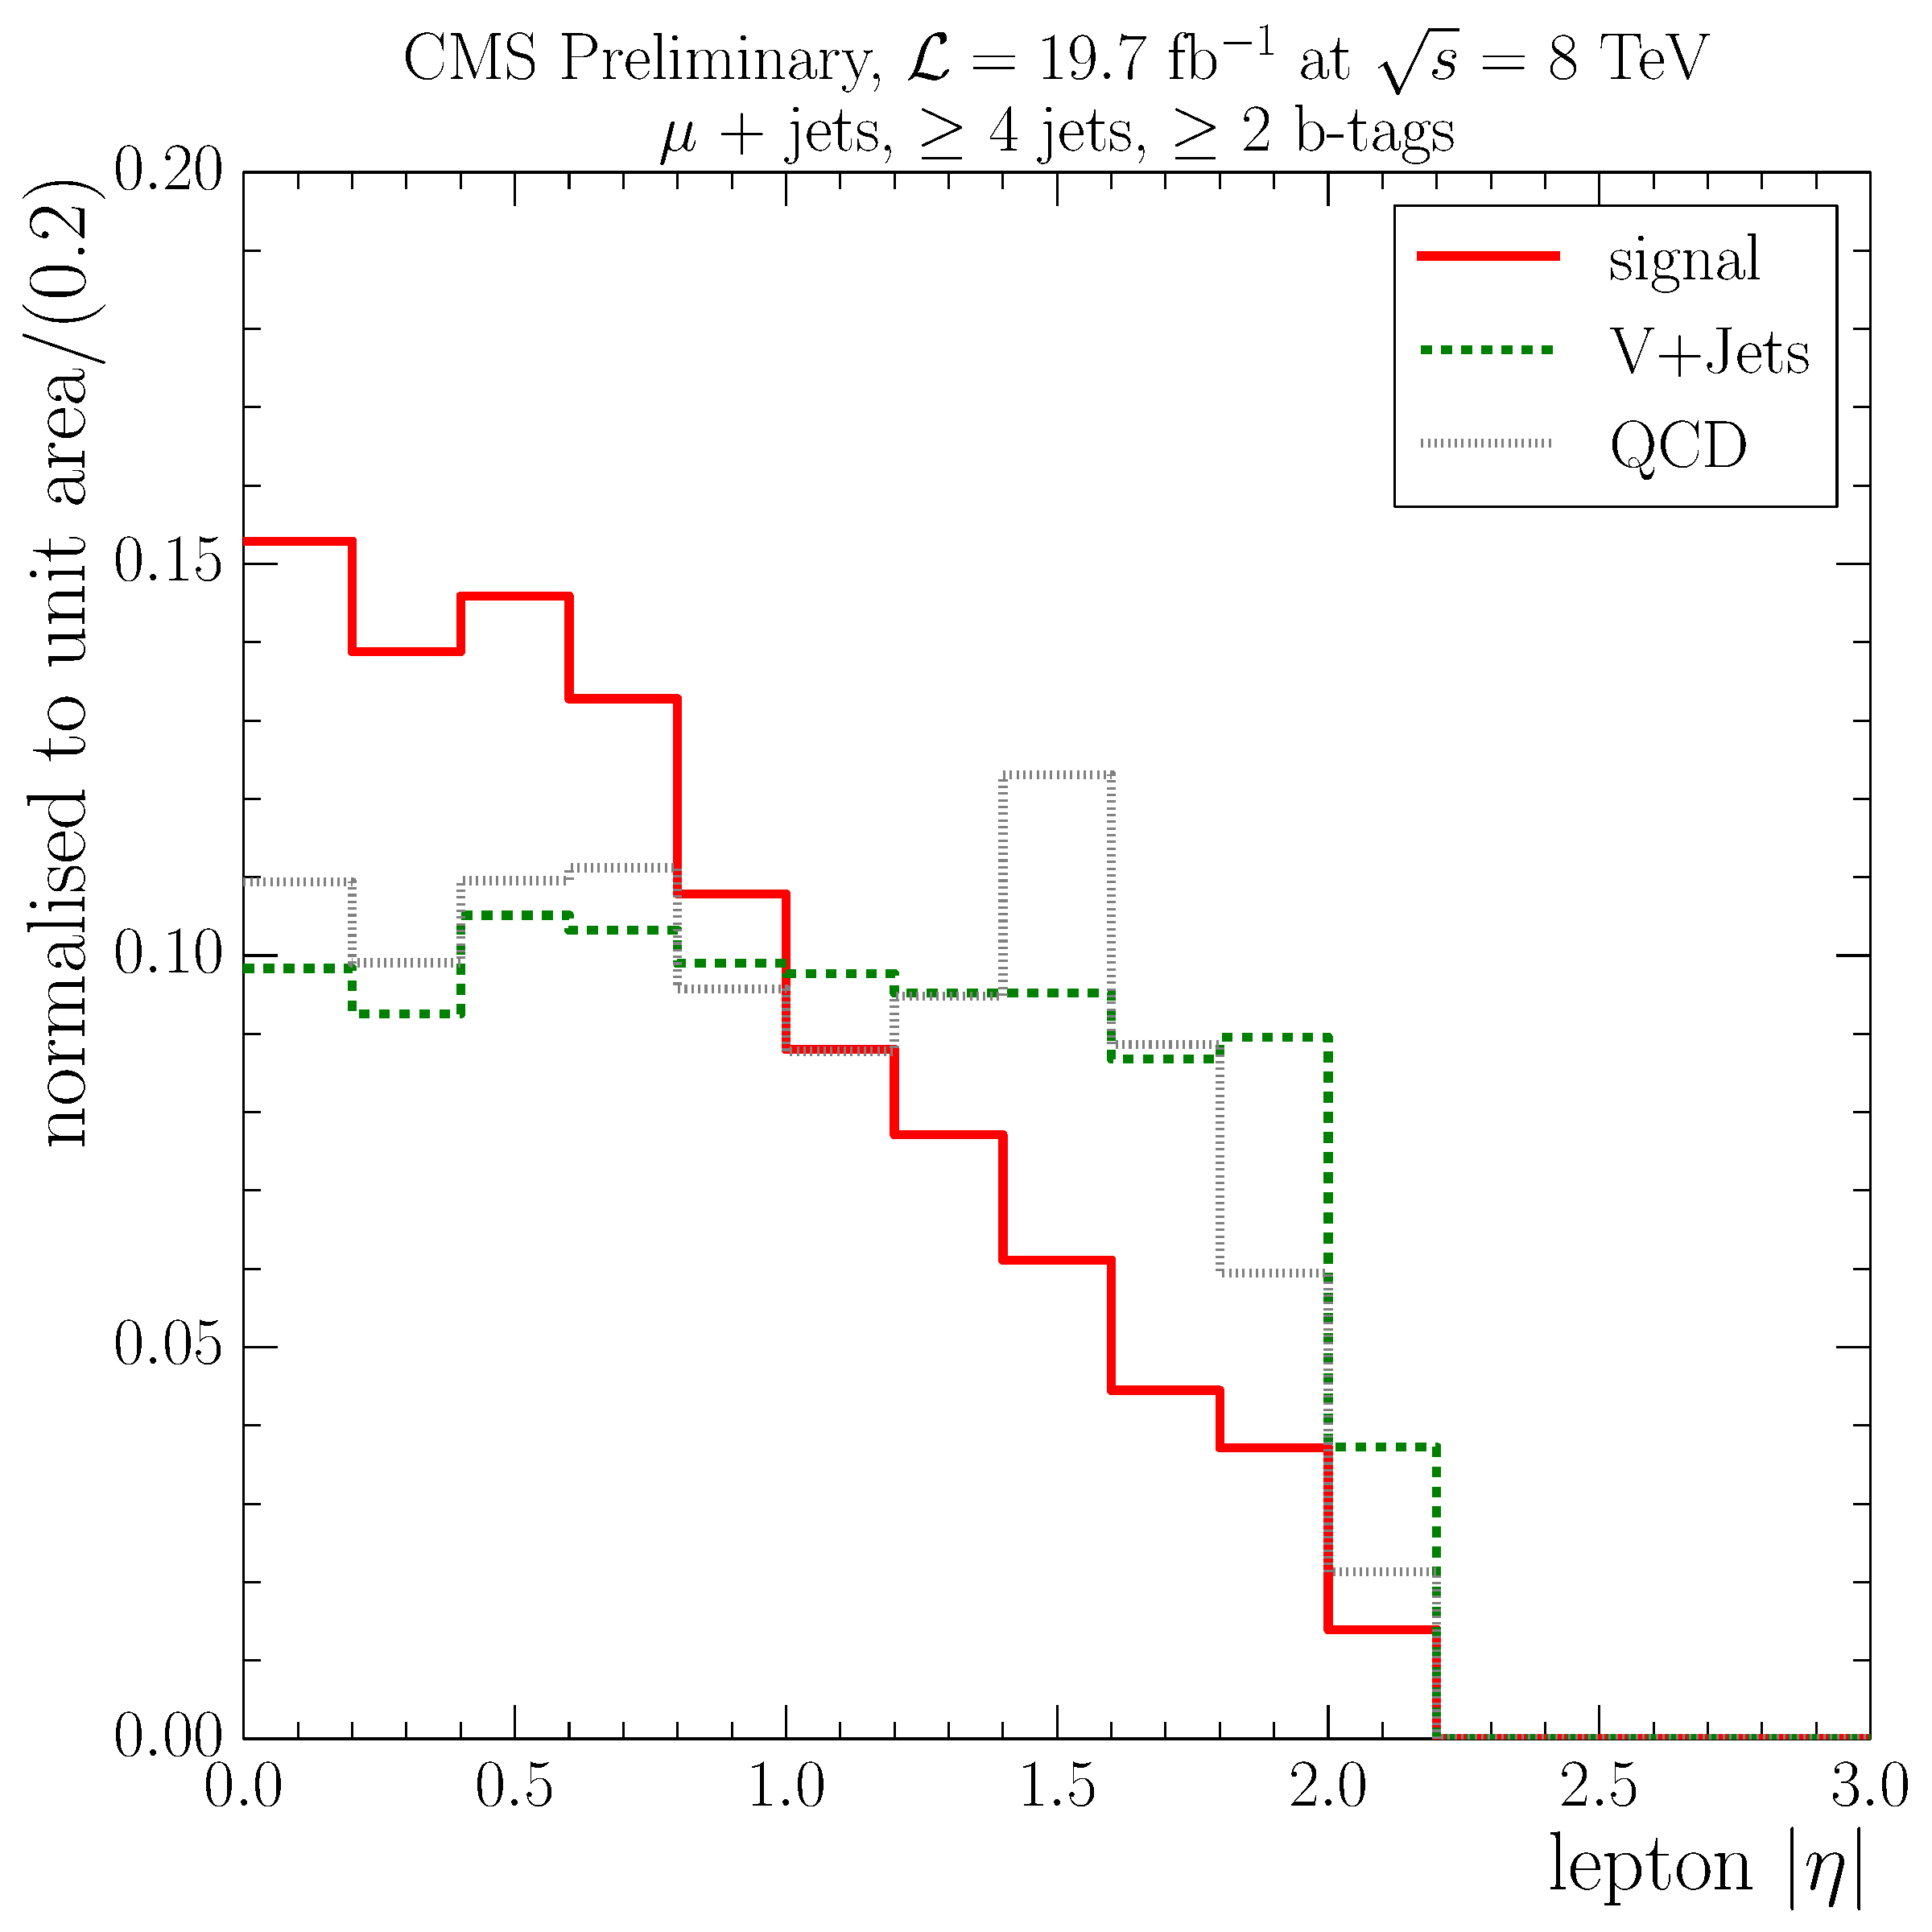
\includegraphics[width=0.3\textwidth]{measurement/HT/central/fit_templates/muon_templates_bin_280-330}}\\
  	{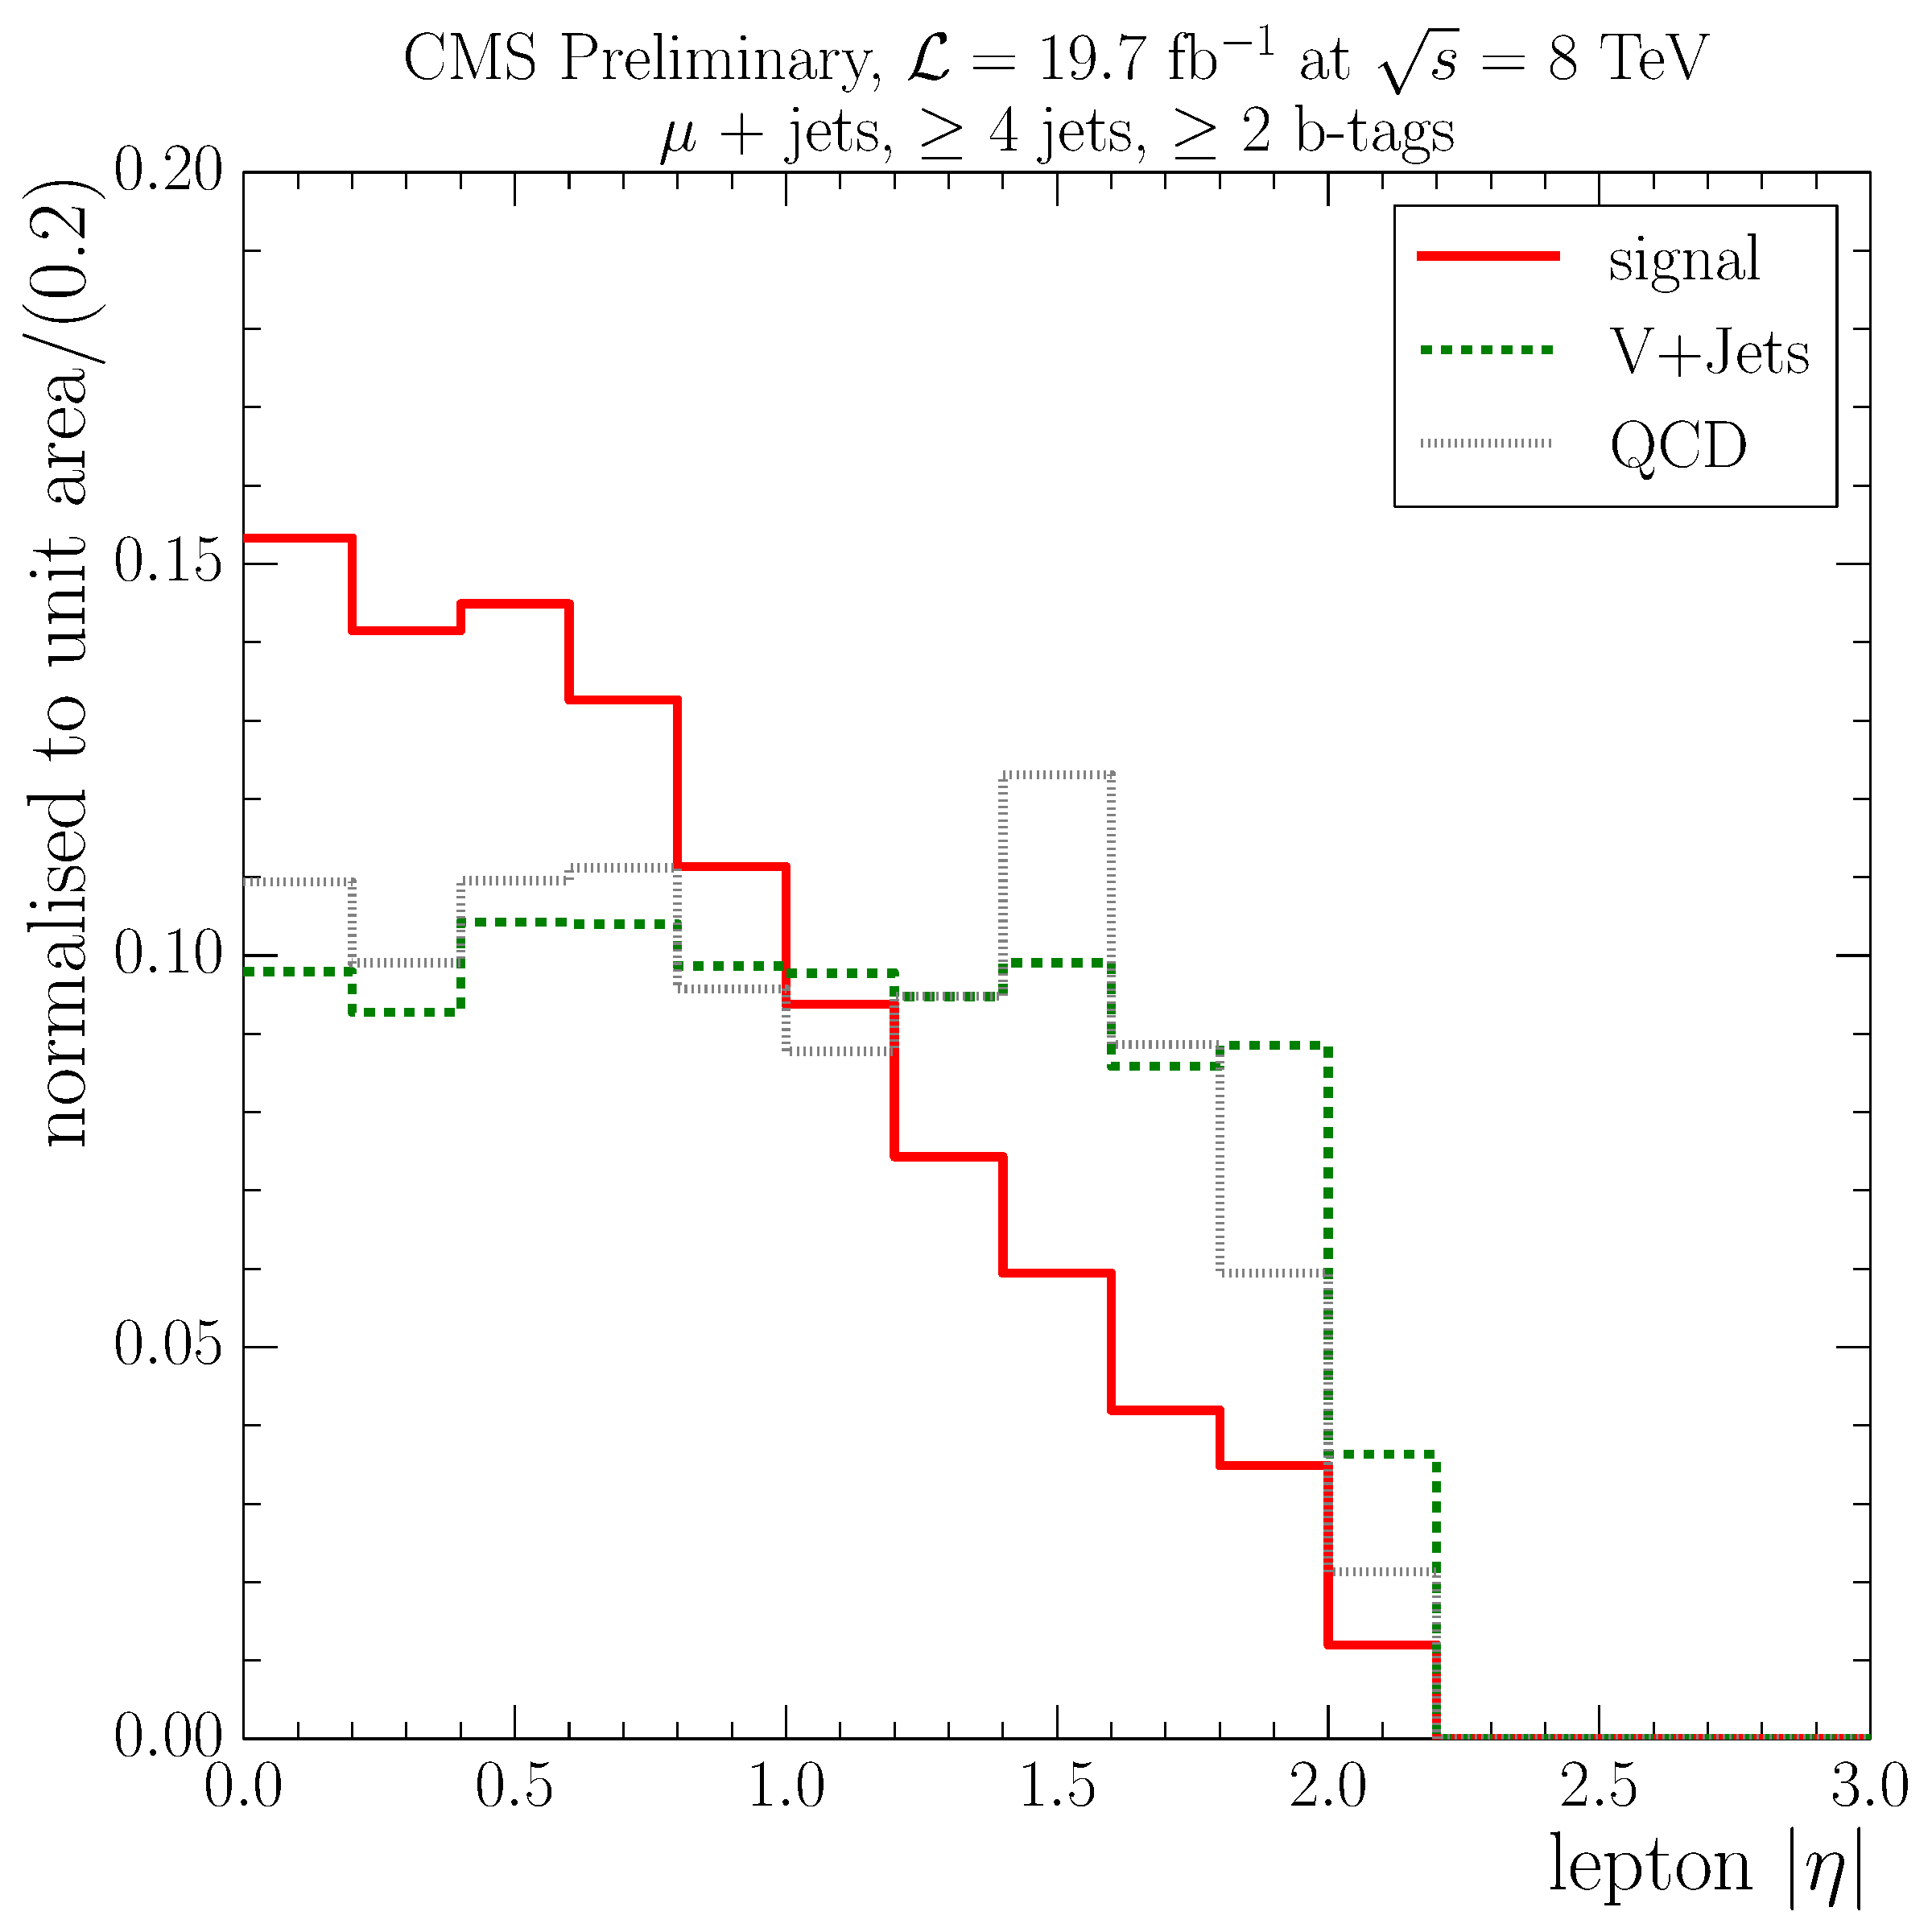
\includegraphics[width=0.3\textwidth]{measurement/HT/central/fit_templates/muon_templates_bin_330-380}}
  	{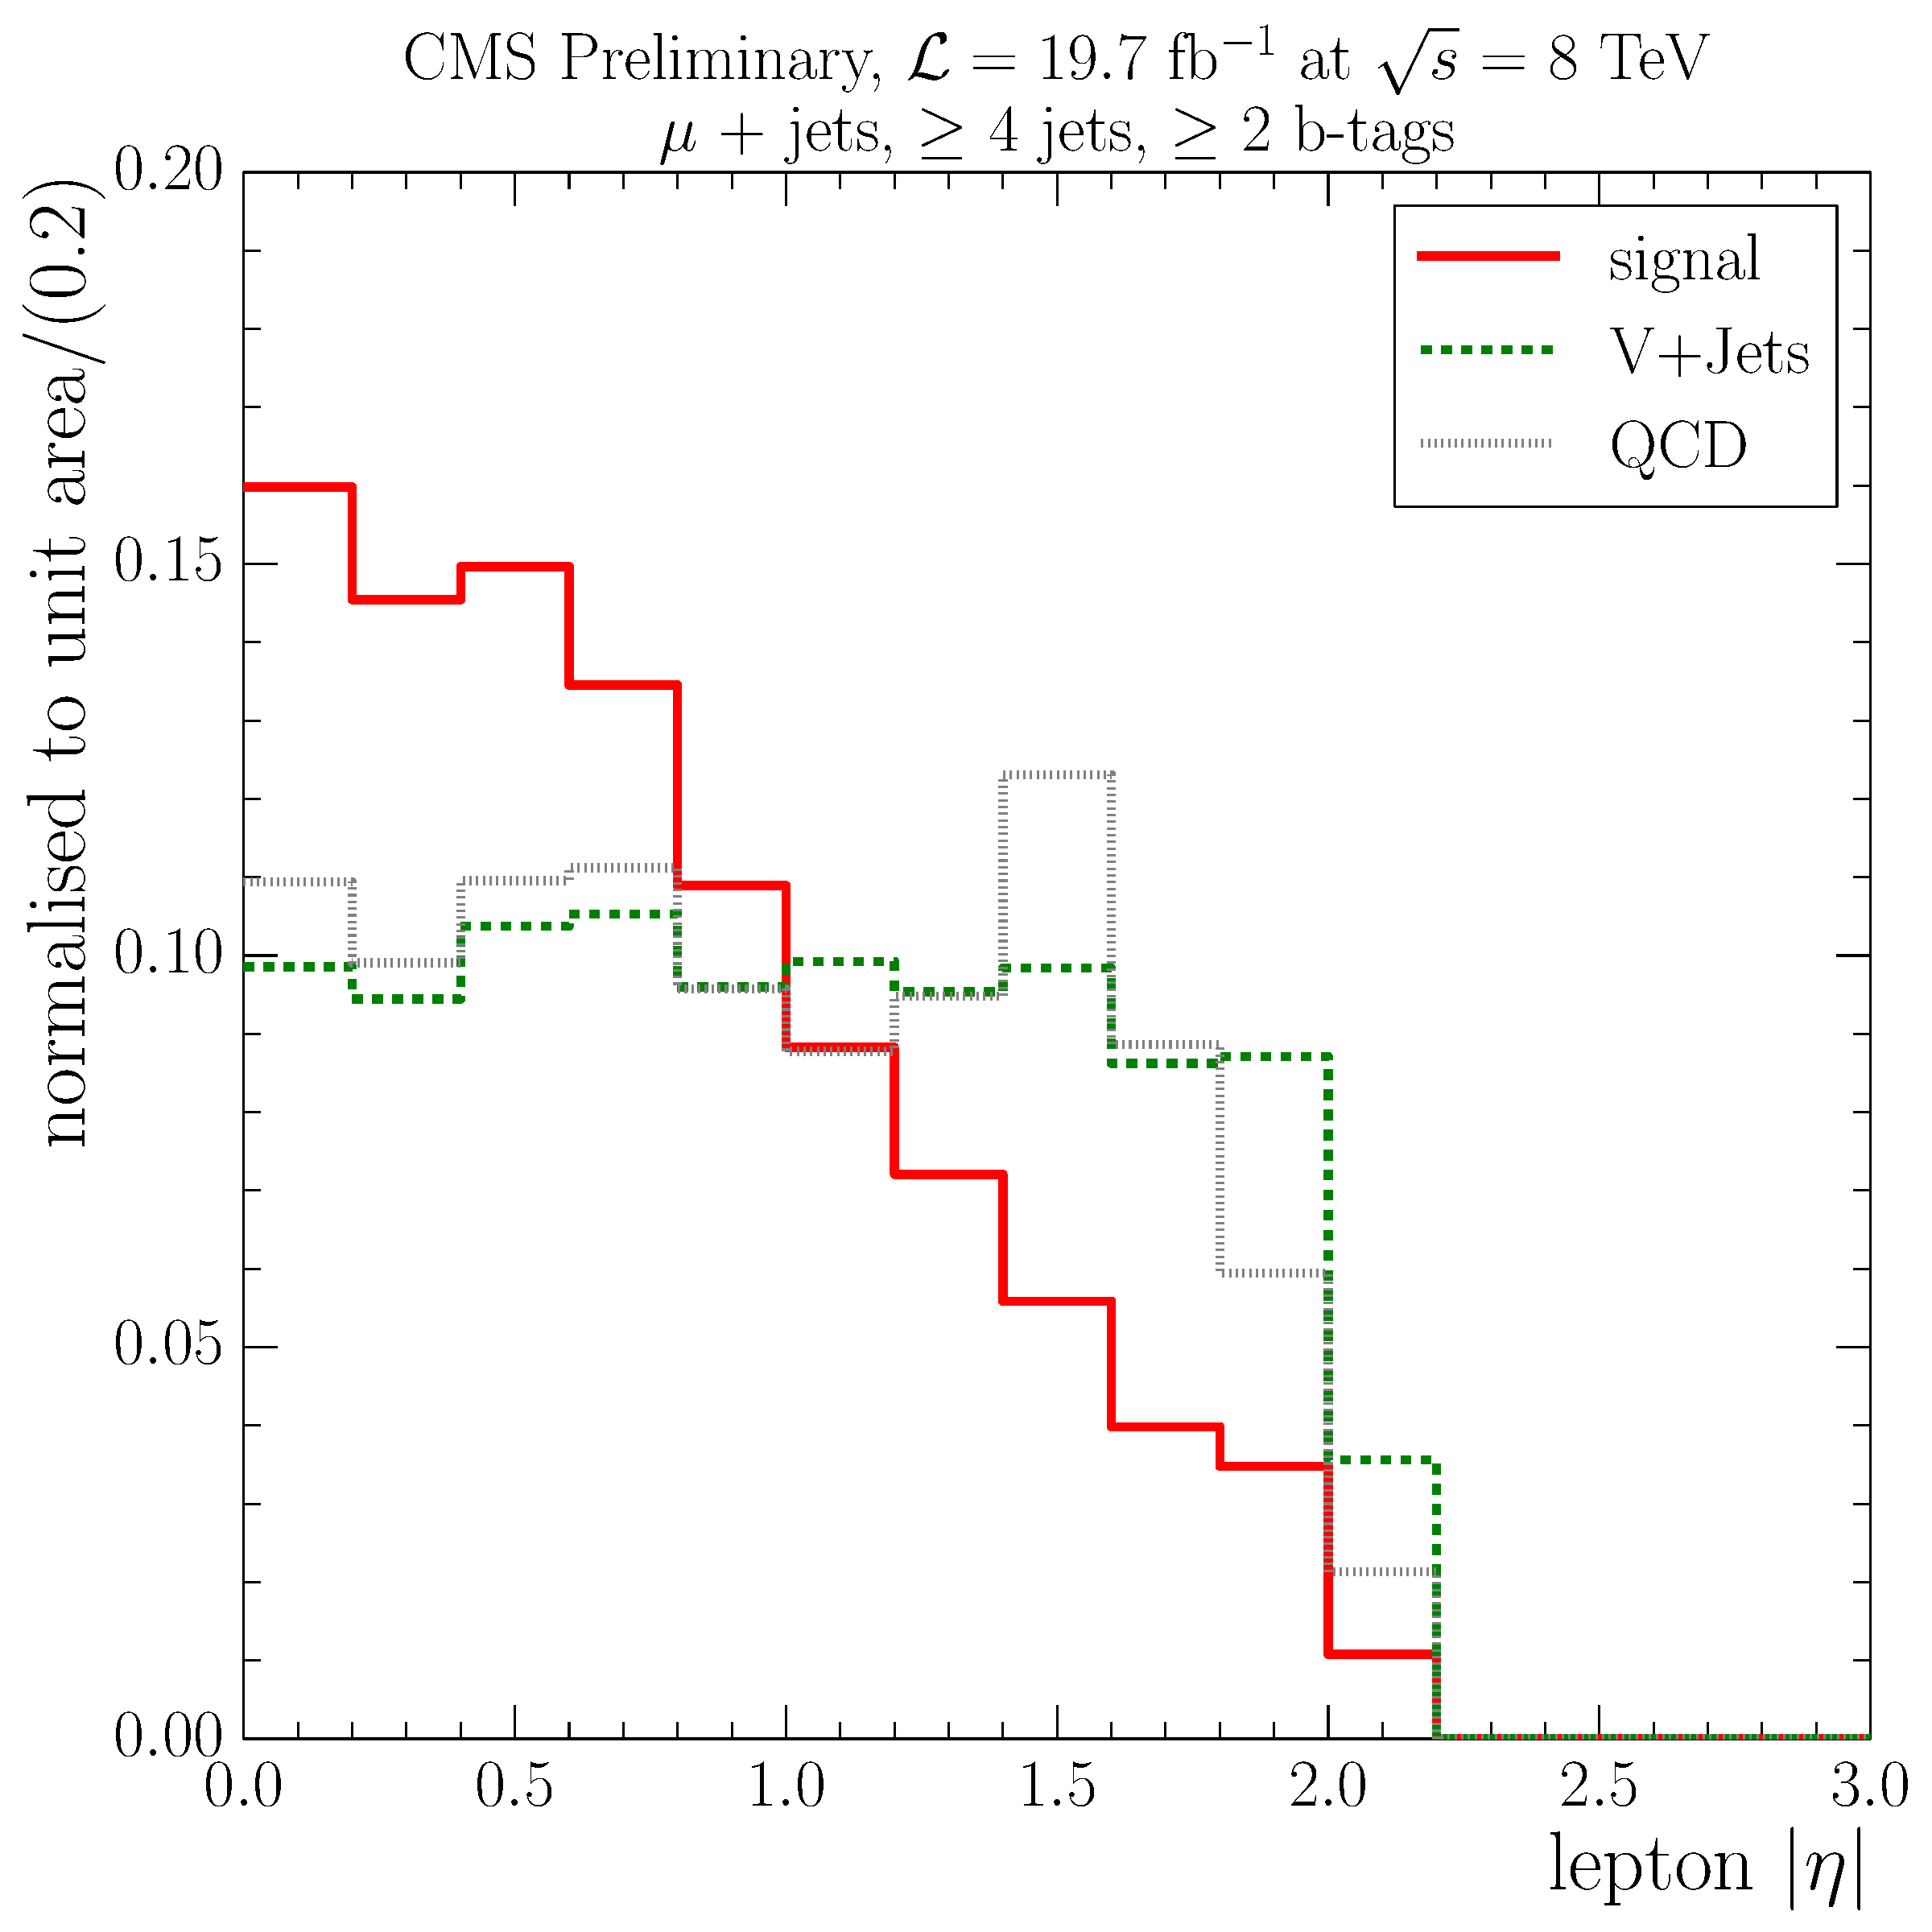
\includegraphics[width=0.3\textwidth]{measurement/HT/central/fit_templates/muon_templates_bin_380-450}}
  	{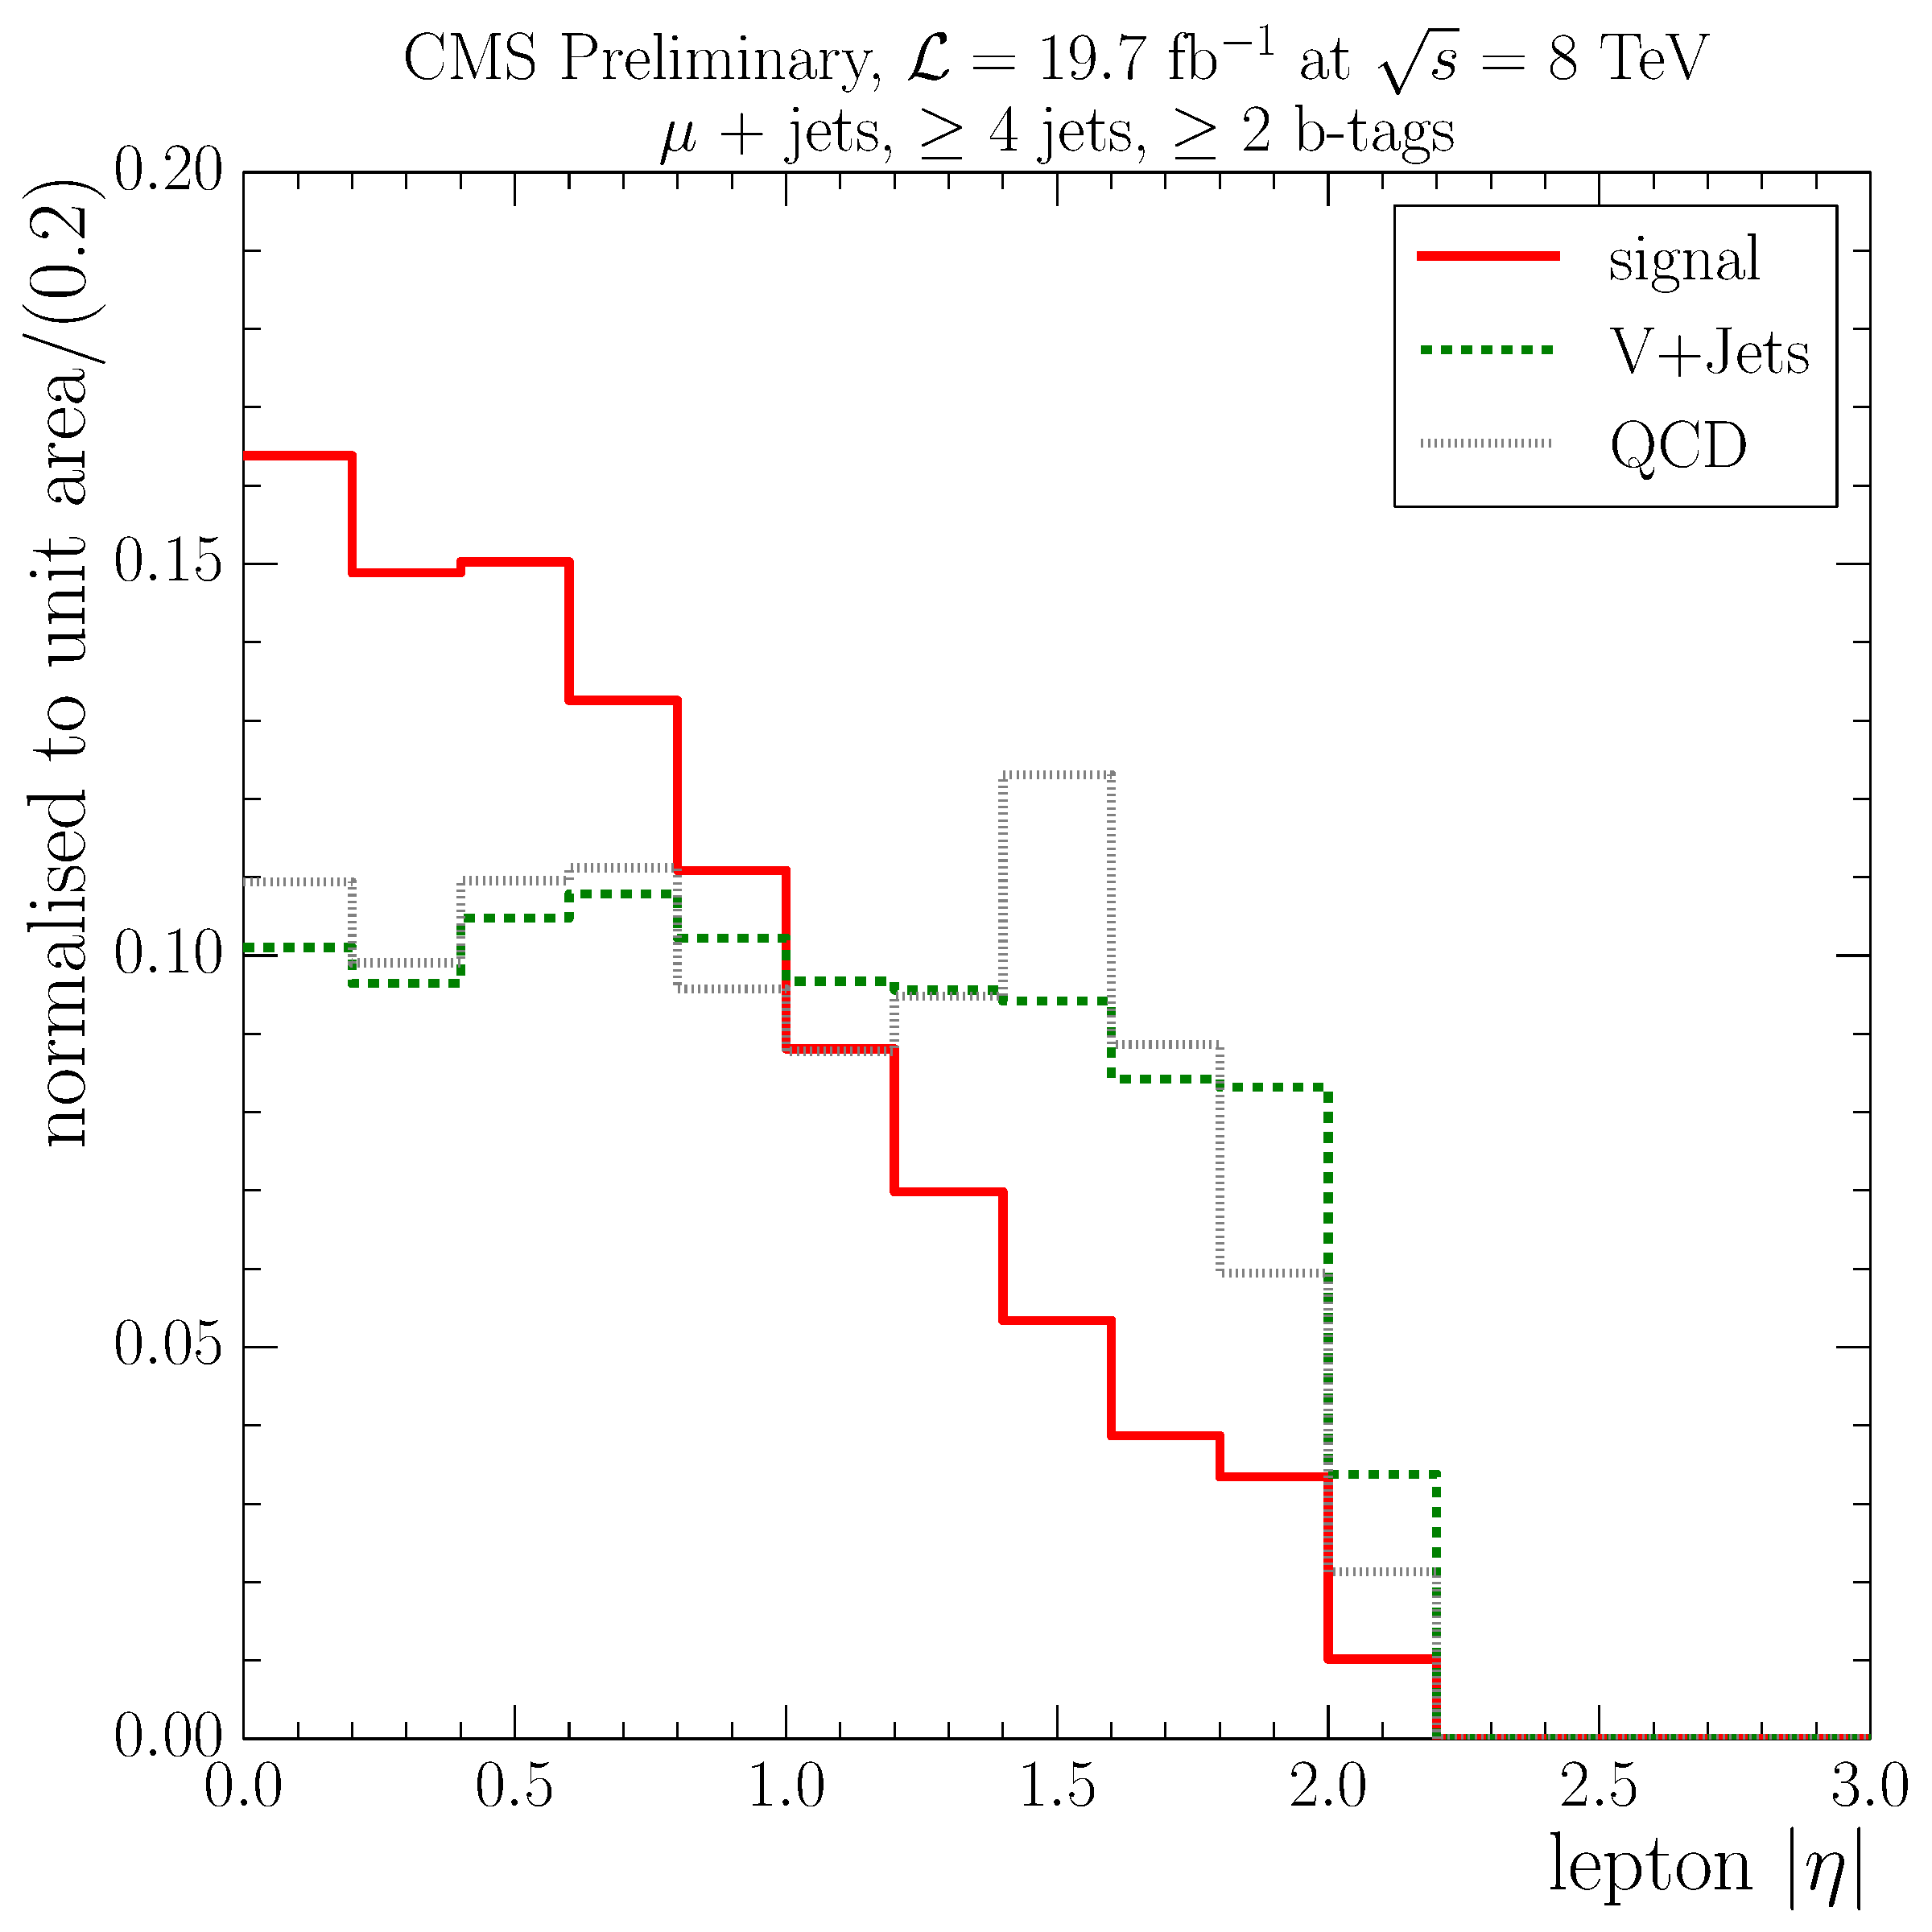
\includegraphics[width=0.3\textwidth]{measurement/HT/central/fit_templates/muon_templates_bin_450-600}}\\
  	{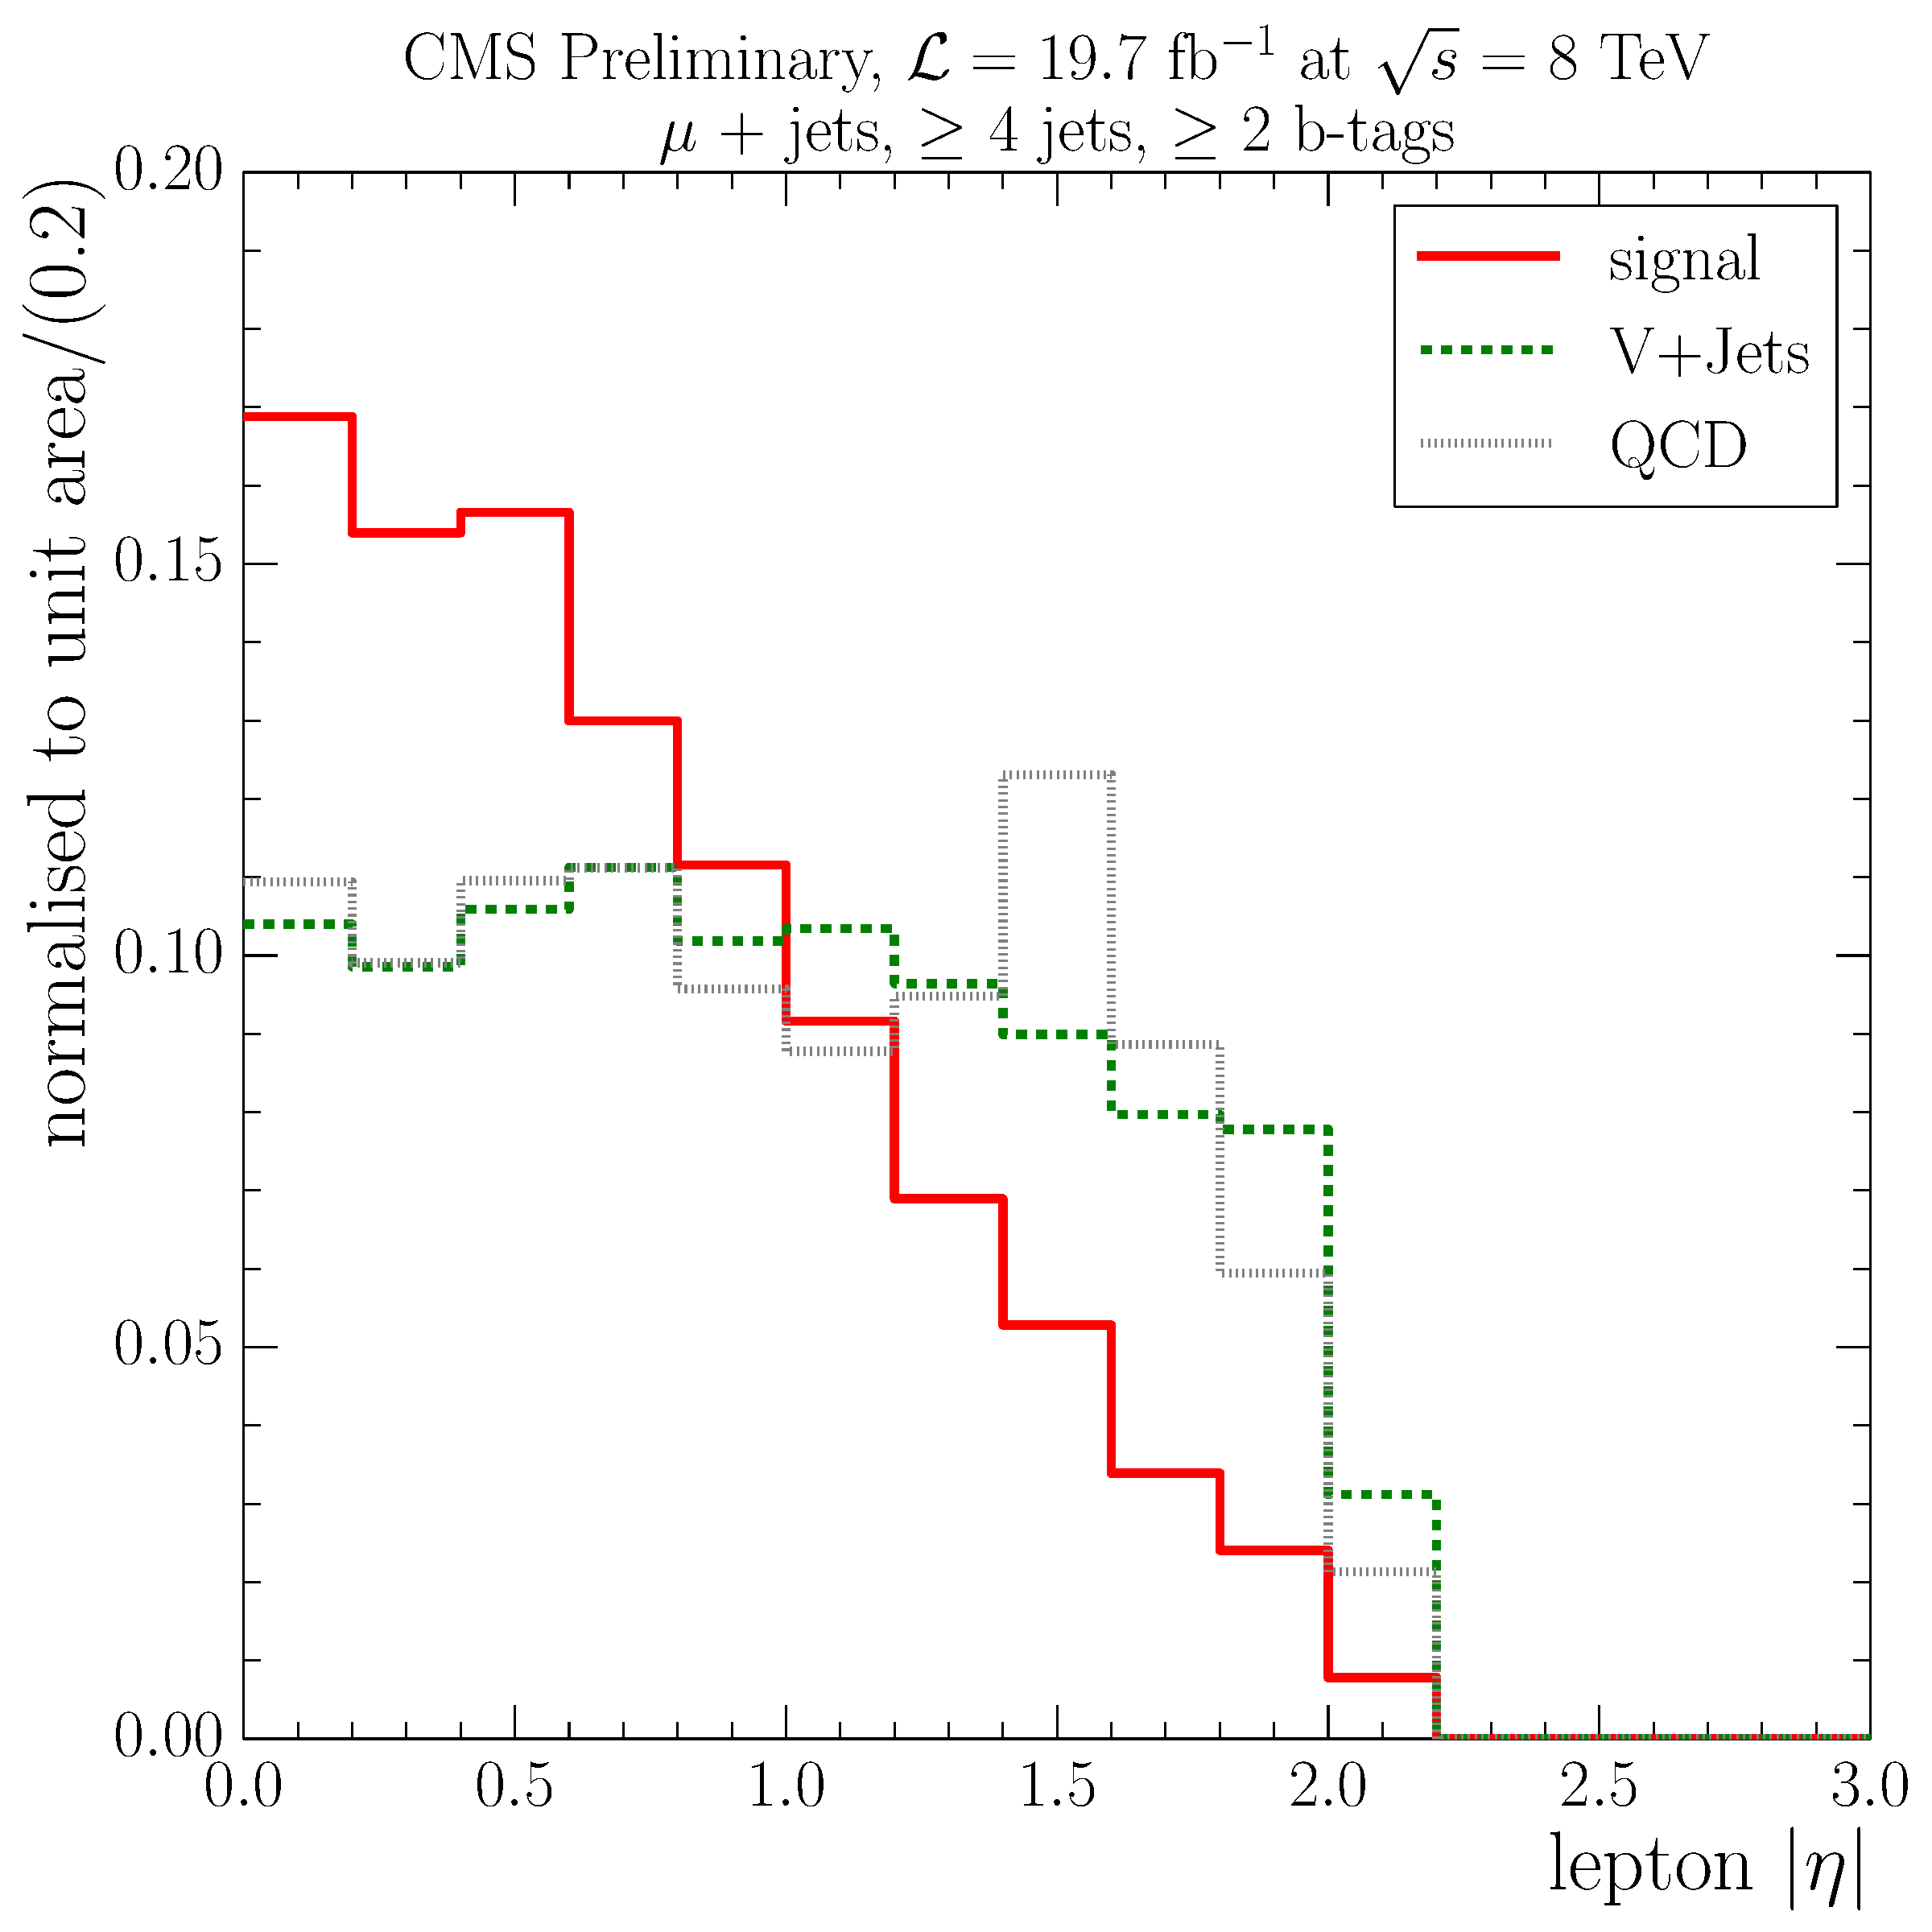
\includegraphics[width=0.3\textwidth]{measurement/HT/central/fit_templates/muon_templates_bin_600-inf}}
    \caption[Muon $\abs \eta$ templates for the fit in different bins of \HT]{Muon $\abs \eta$ templates for the fit in
    different bins of \HT, from top left to bottom: \SIrange{0}{240}{\GeV}, \SIrange{240}{280}{\GeV},
    \SIrange{280}{330}{\GeV}, \SIrange{330}{380}{\GeV}, \SIrange{380}{450}{\GeV}, \SIrange{450}{600}{\GeV} and $\geq
    \SI{600}{\GeV}$.}
    \label{fig:fit_templates_HT_muon}
\end{figure}

\newpage
\section*{\ST variable}

\begin{figure}[!htbp]
  \centering
    {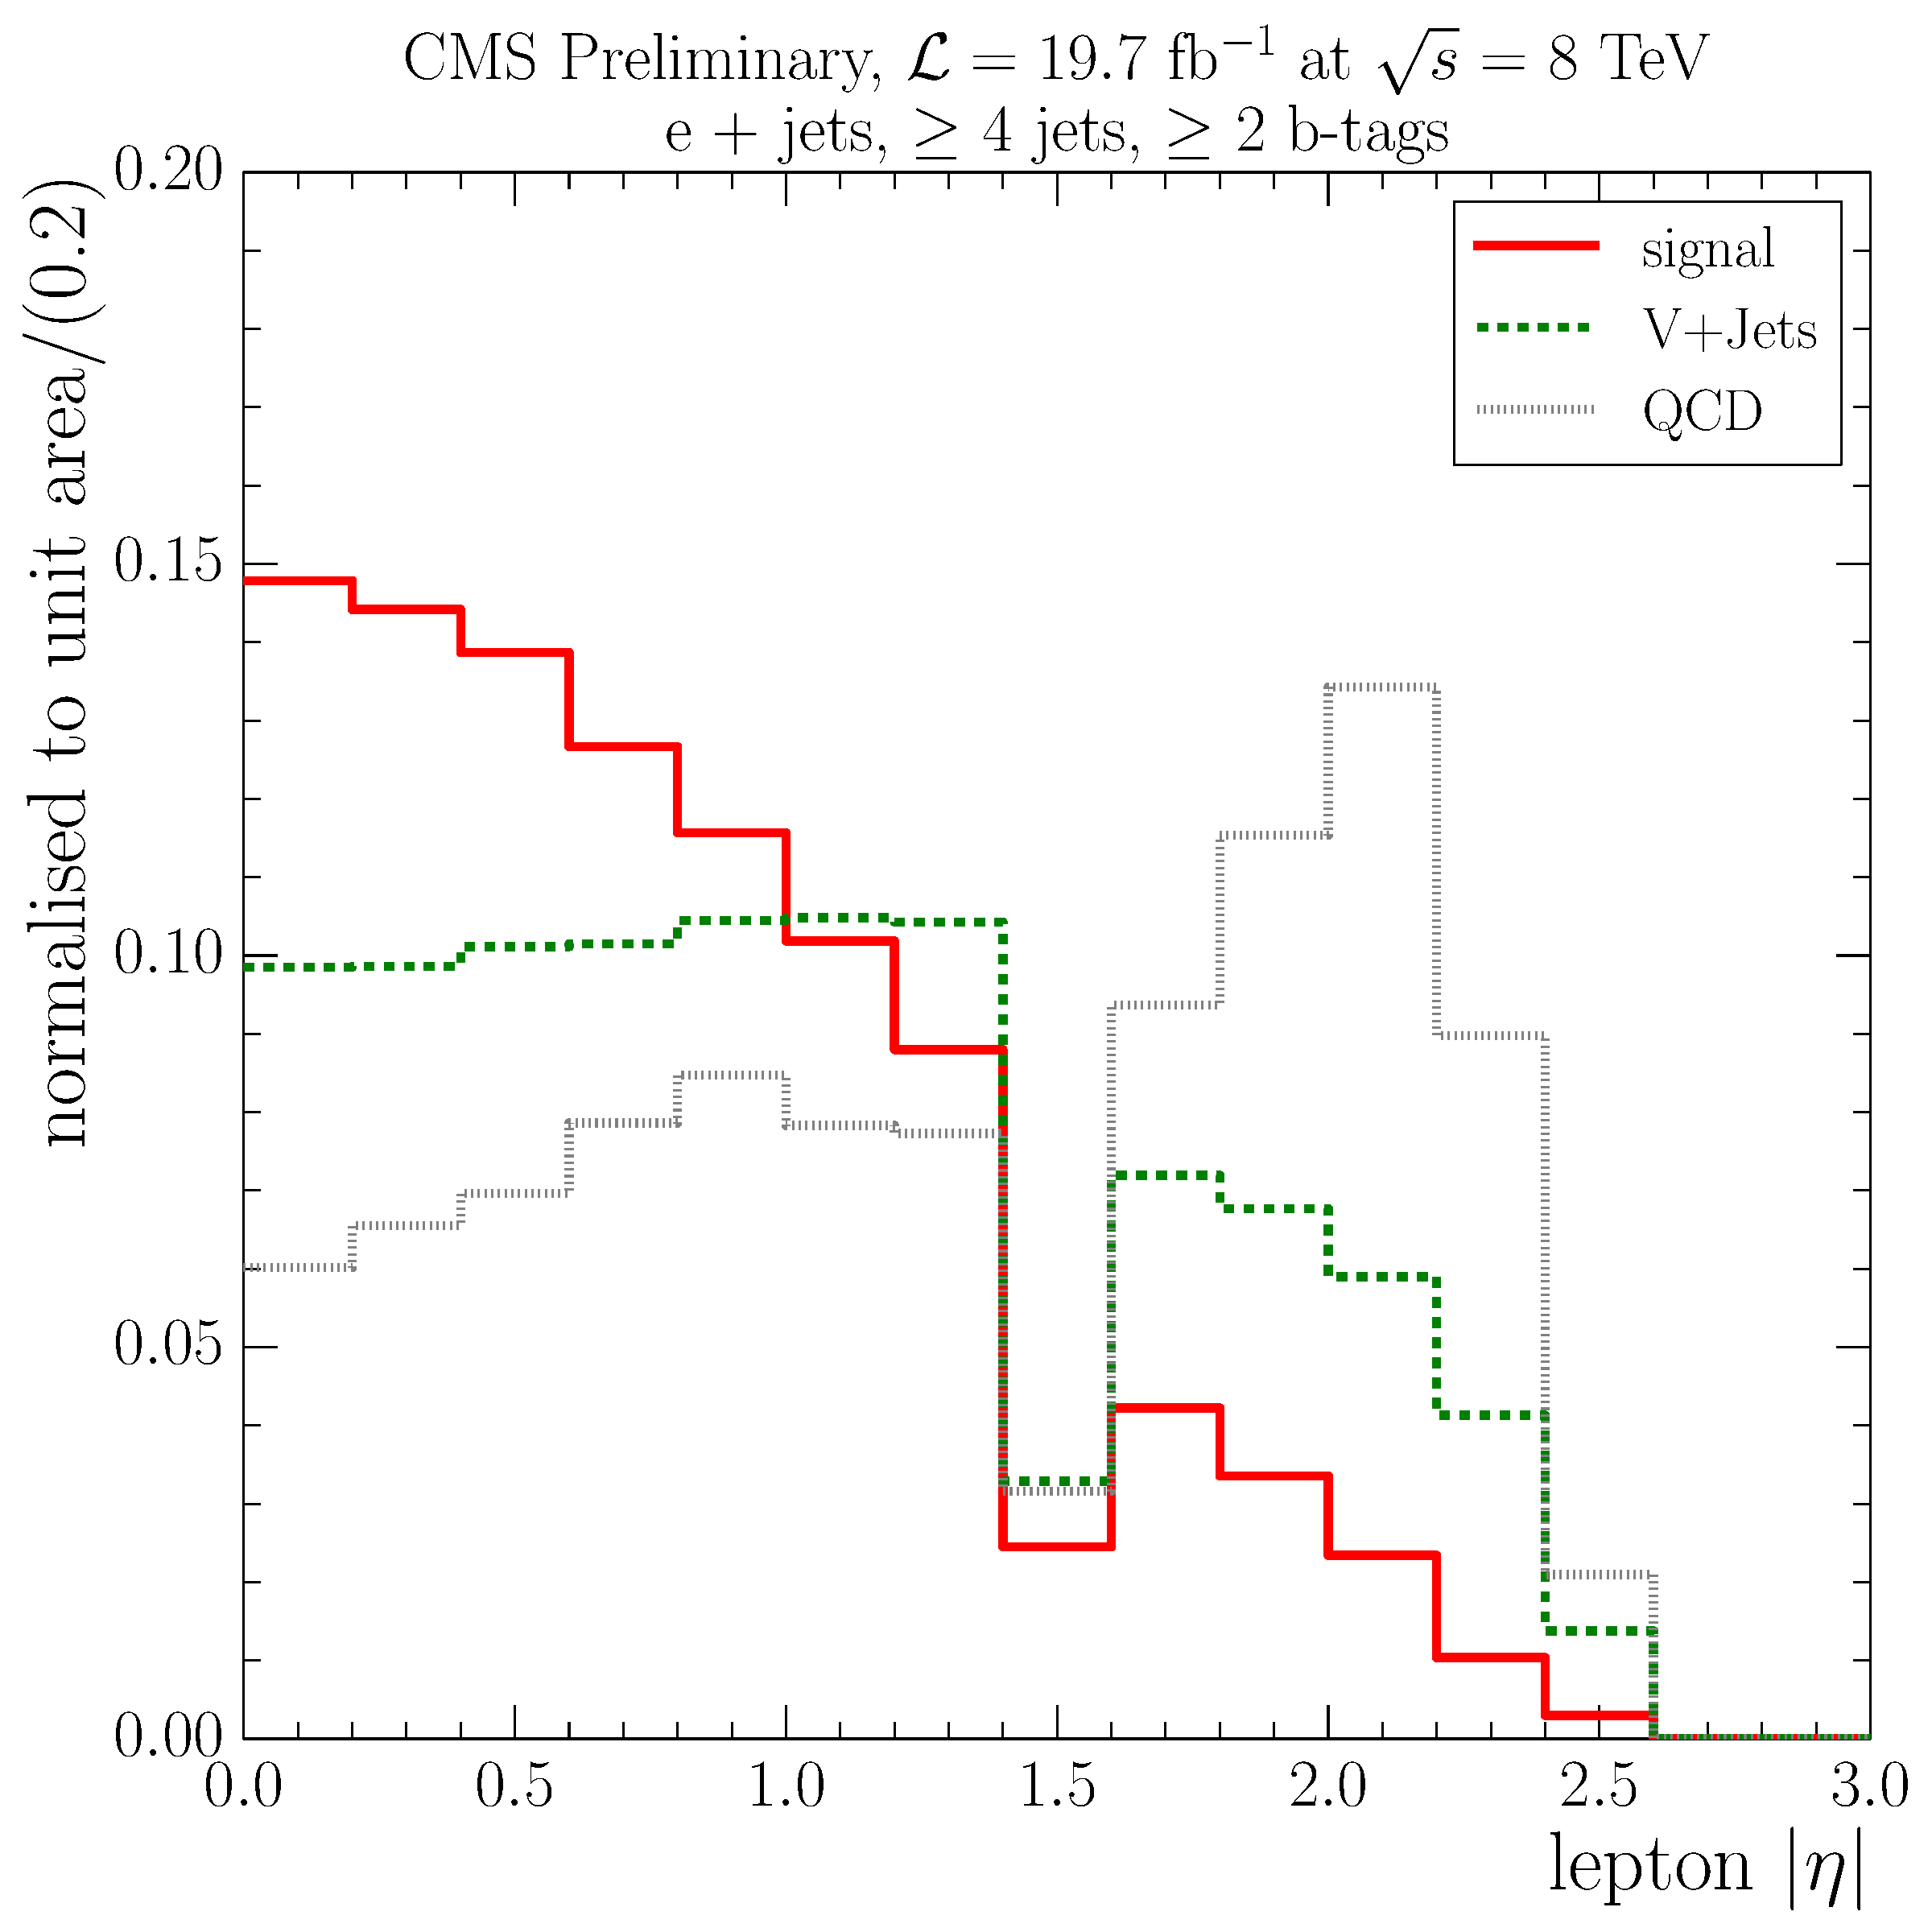
\includegraphics[width=0.3\textwidth]{measurement/ST/central/fit_templates/electron_templates_bin_0-350}}
    {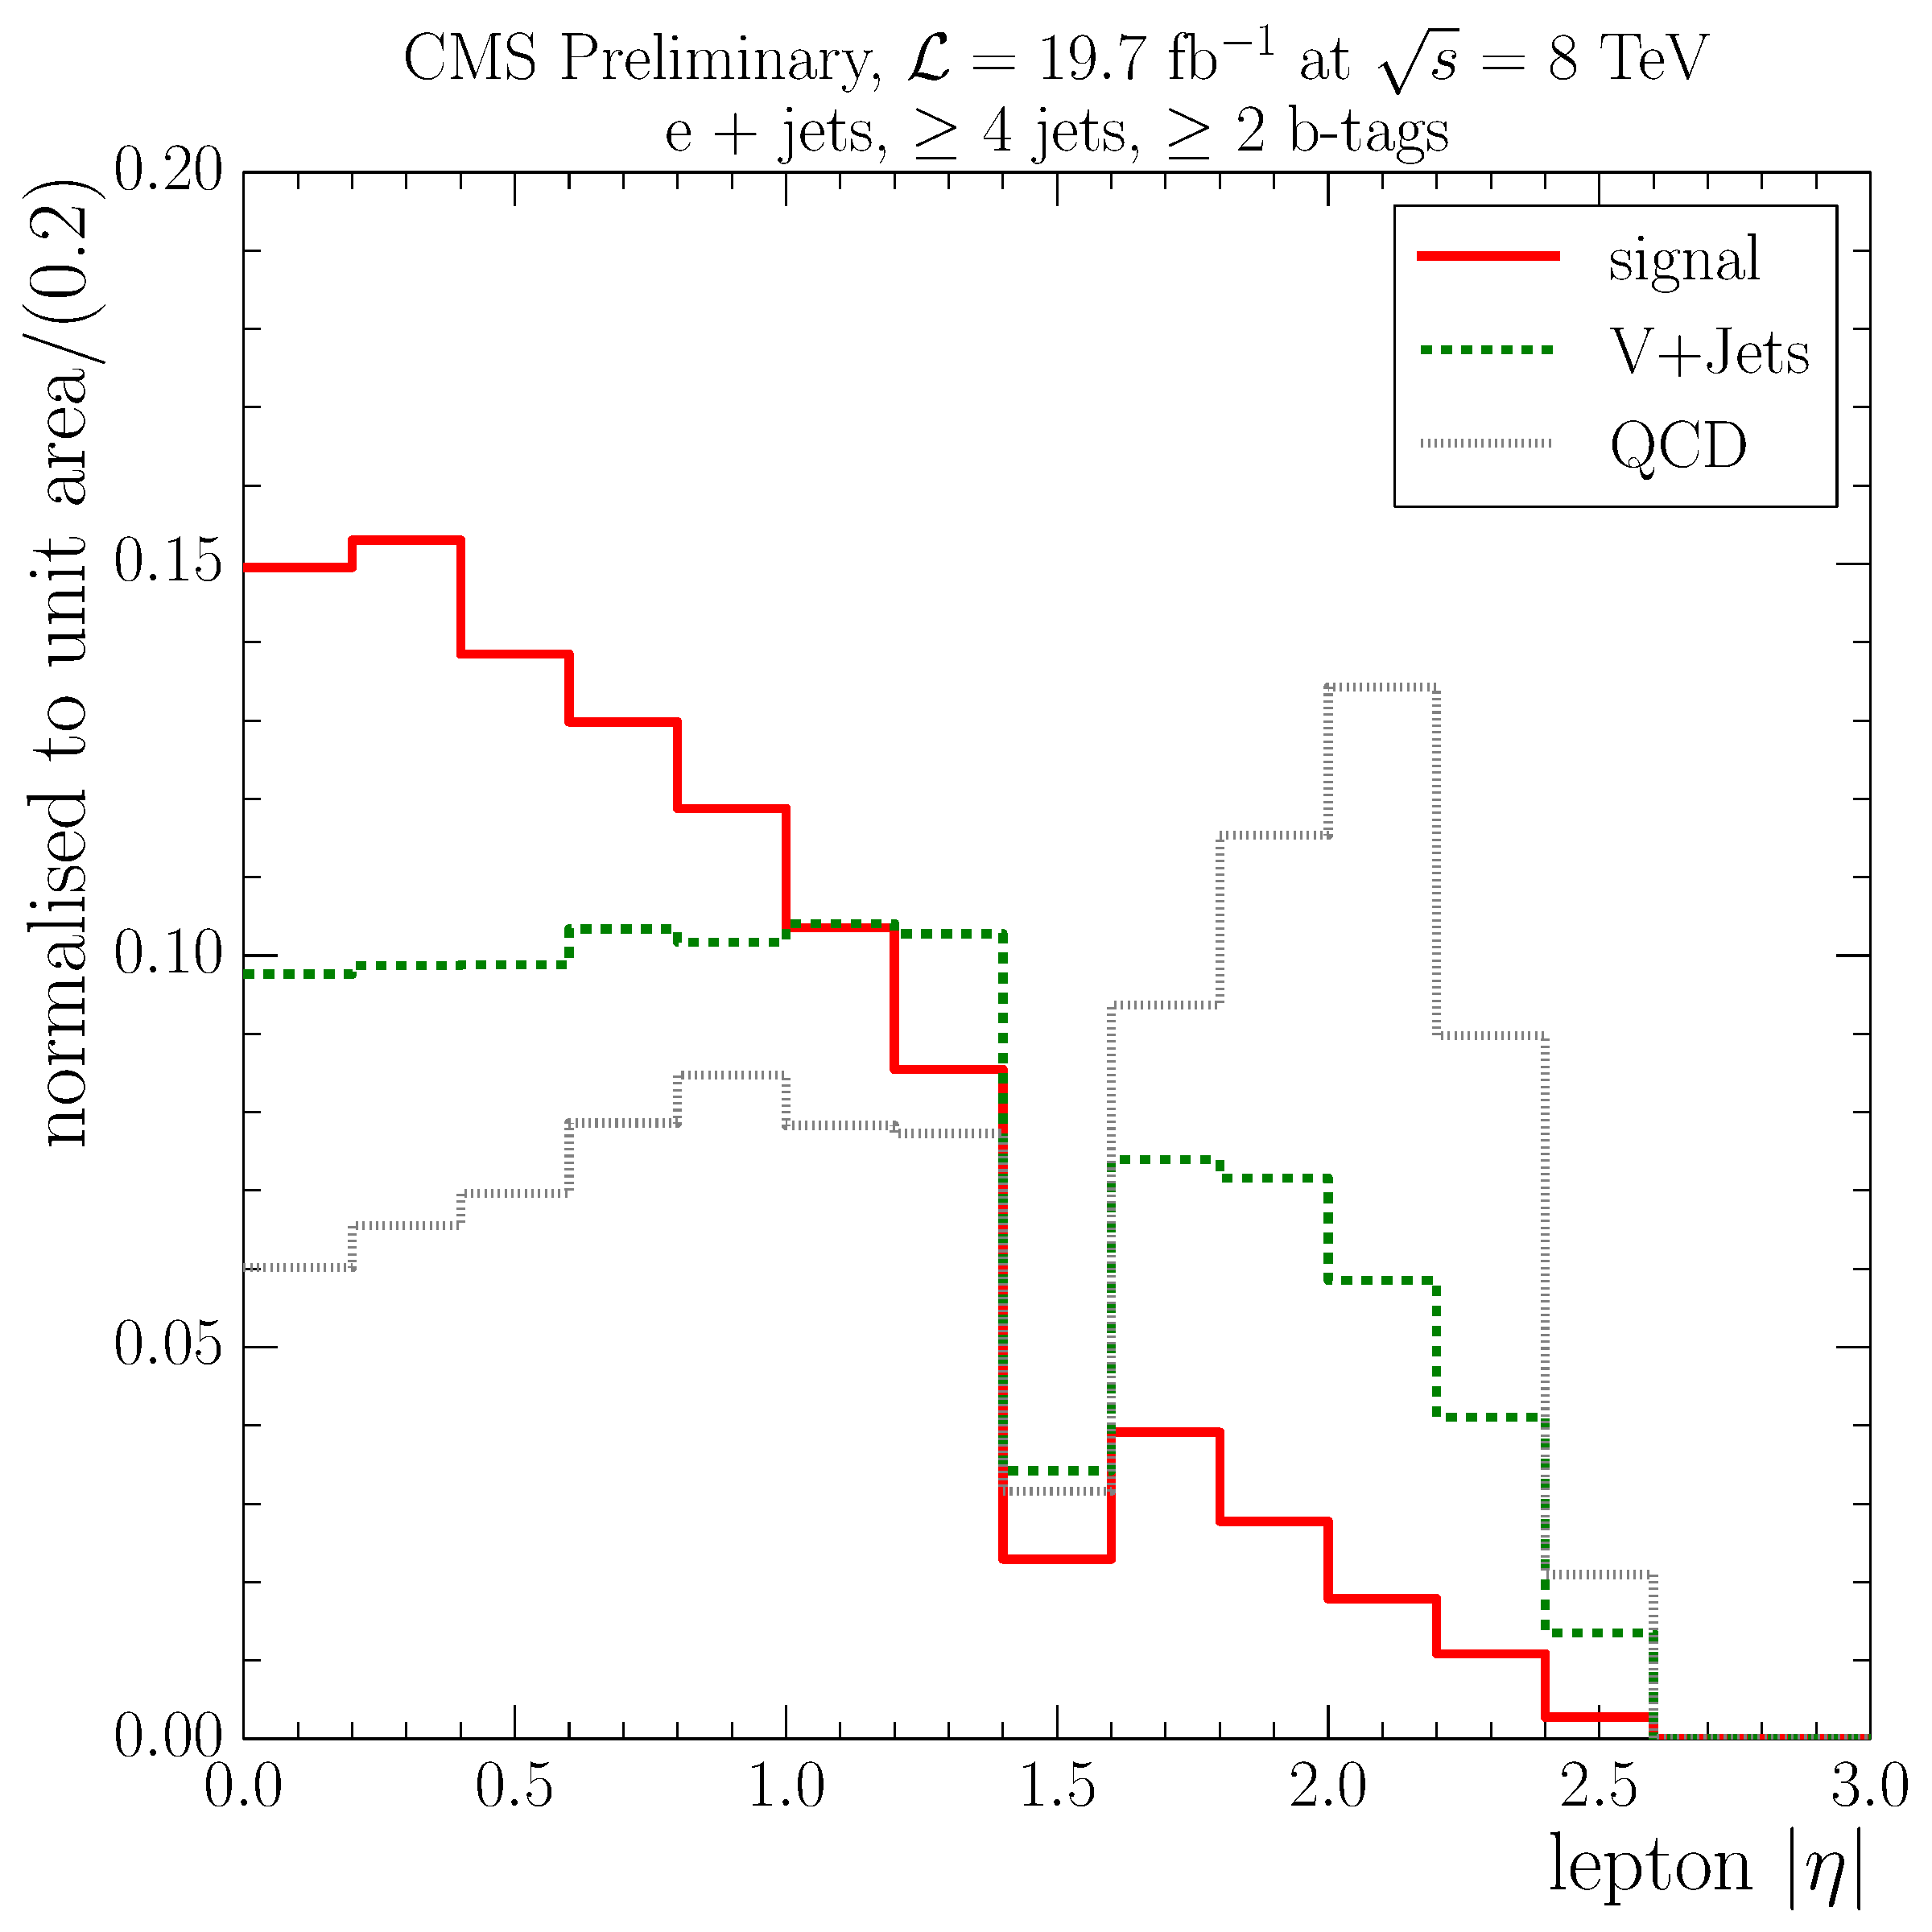
\includegraphics[width=0.3\textwidth]{measurement/ST/central/fit_templates/electron_templates_bin_350-400}}
    {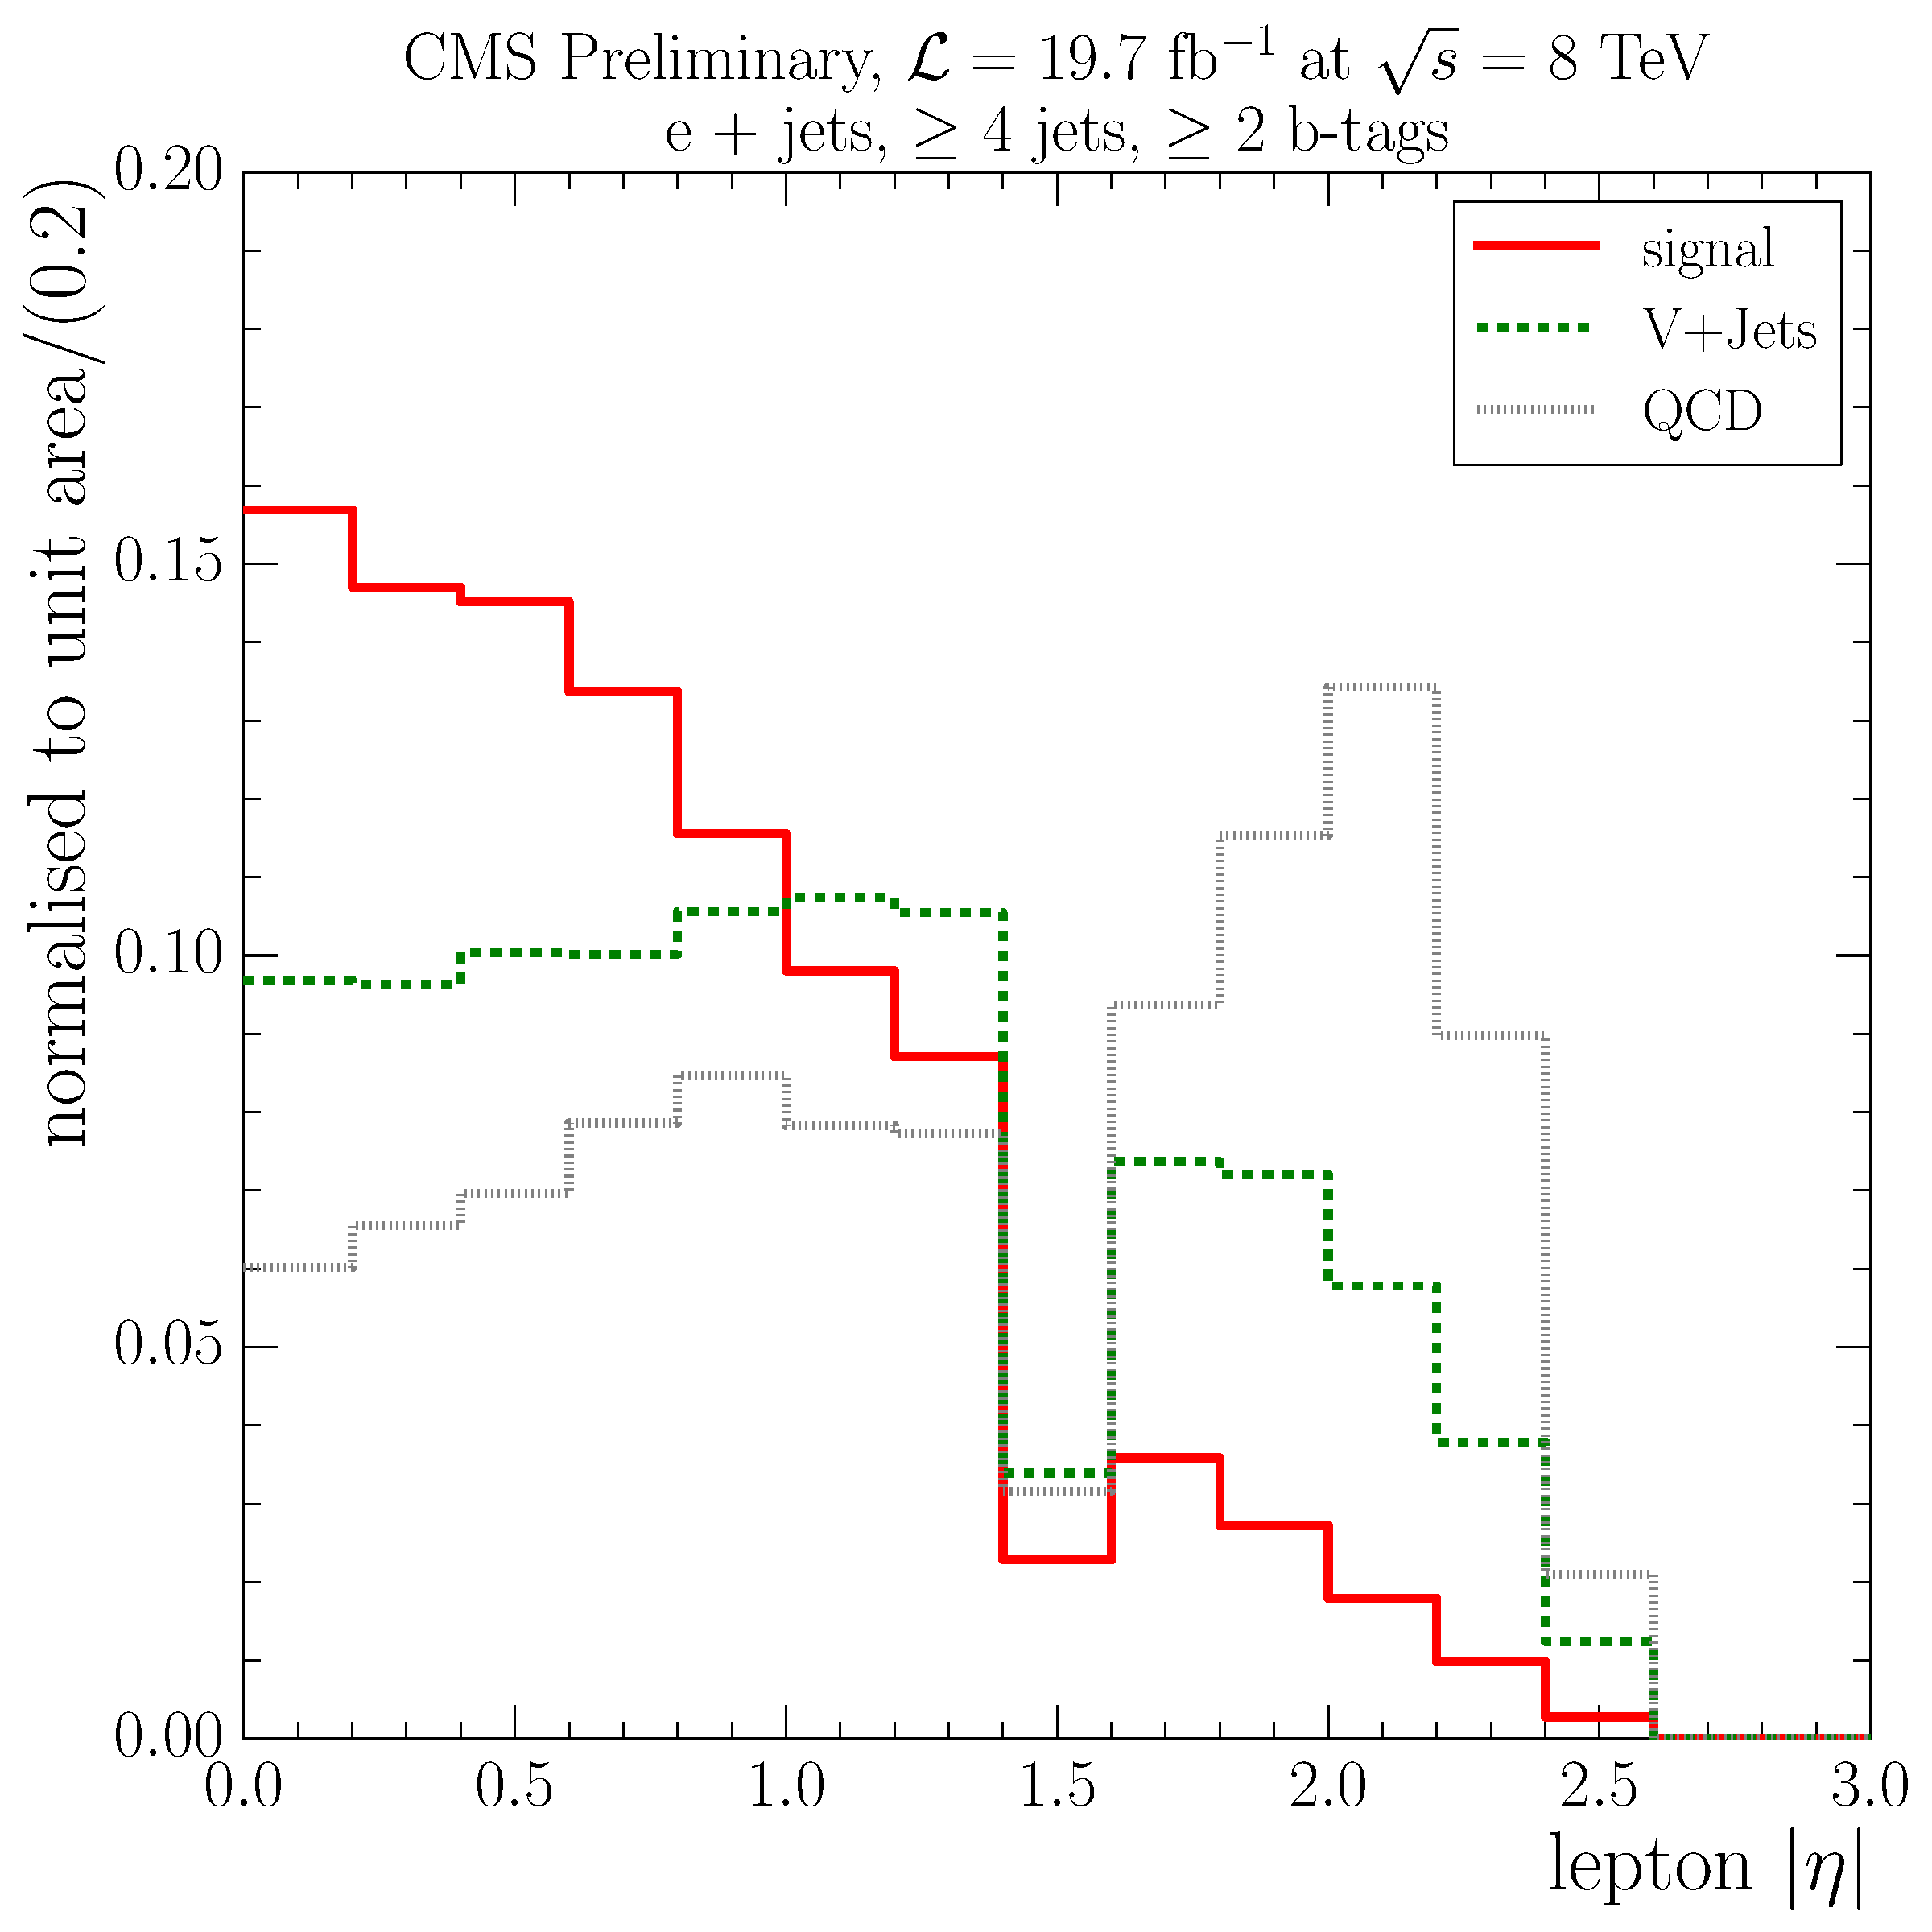
\includegraphics[width=0.3\textwidth]{measurement/ST/central/fit_templates/electron_templates_bin_400-450}}\\
    {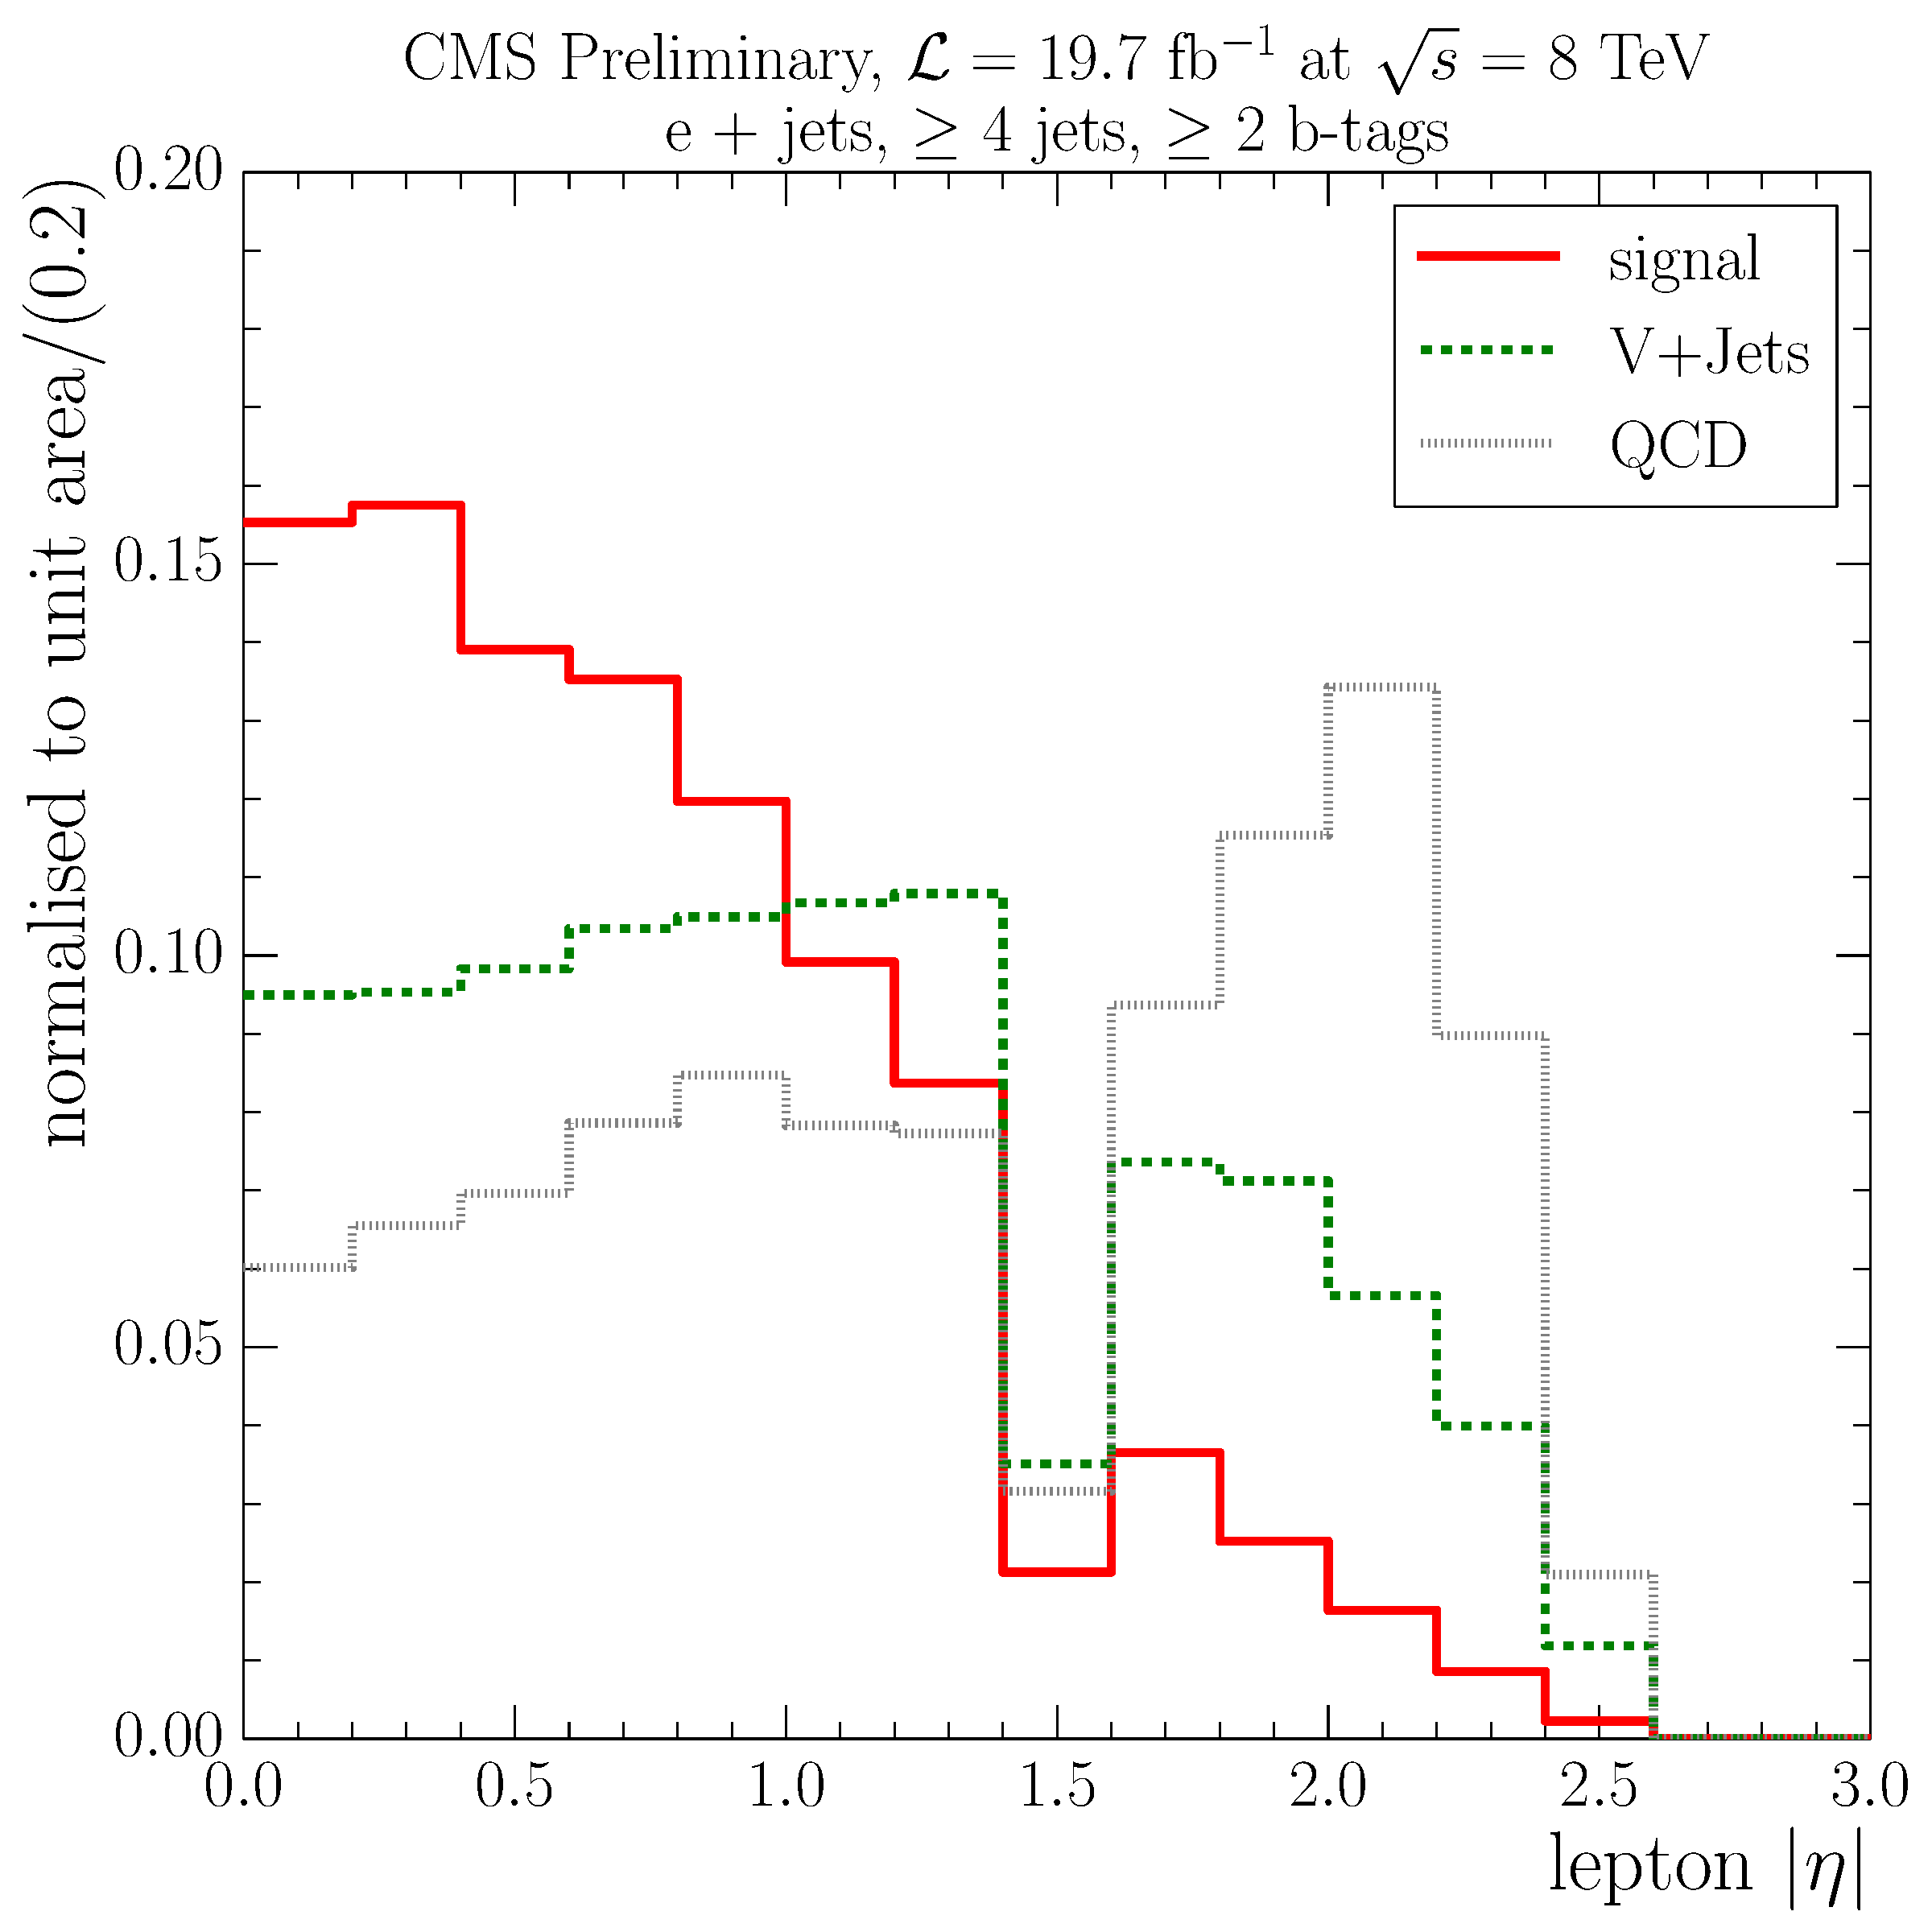
\includegraphics[width=0.3\textwidth]{measurement/ST/central/fit_templates/electron_templates_bin_450-500}}
    {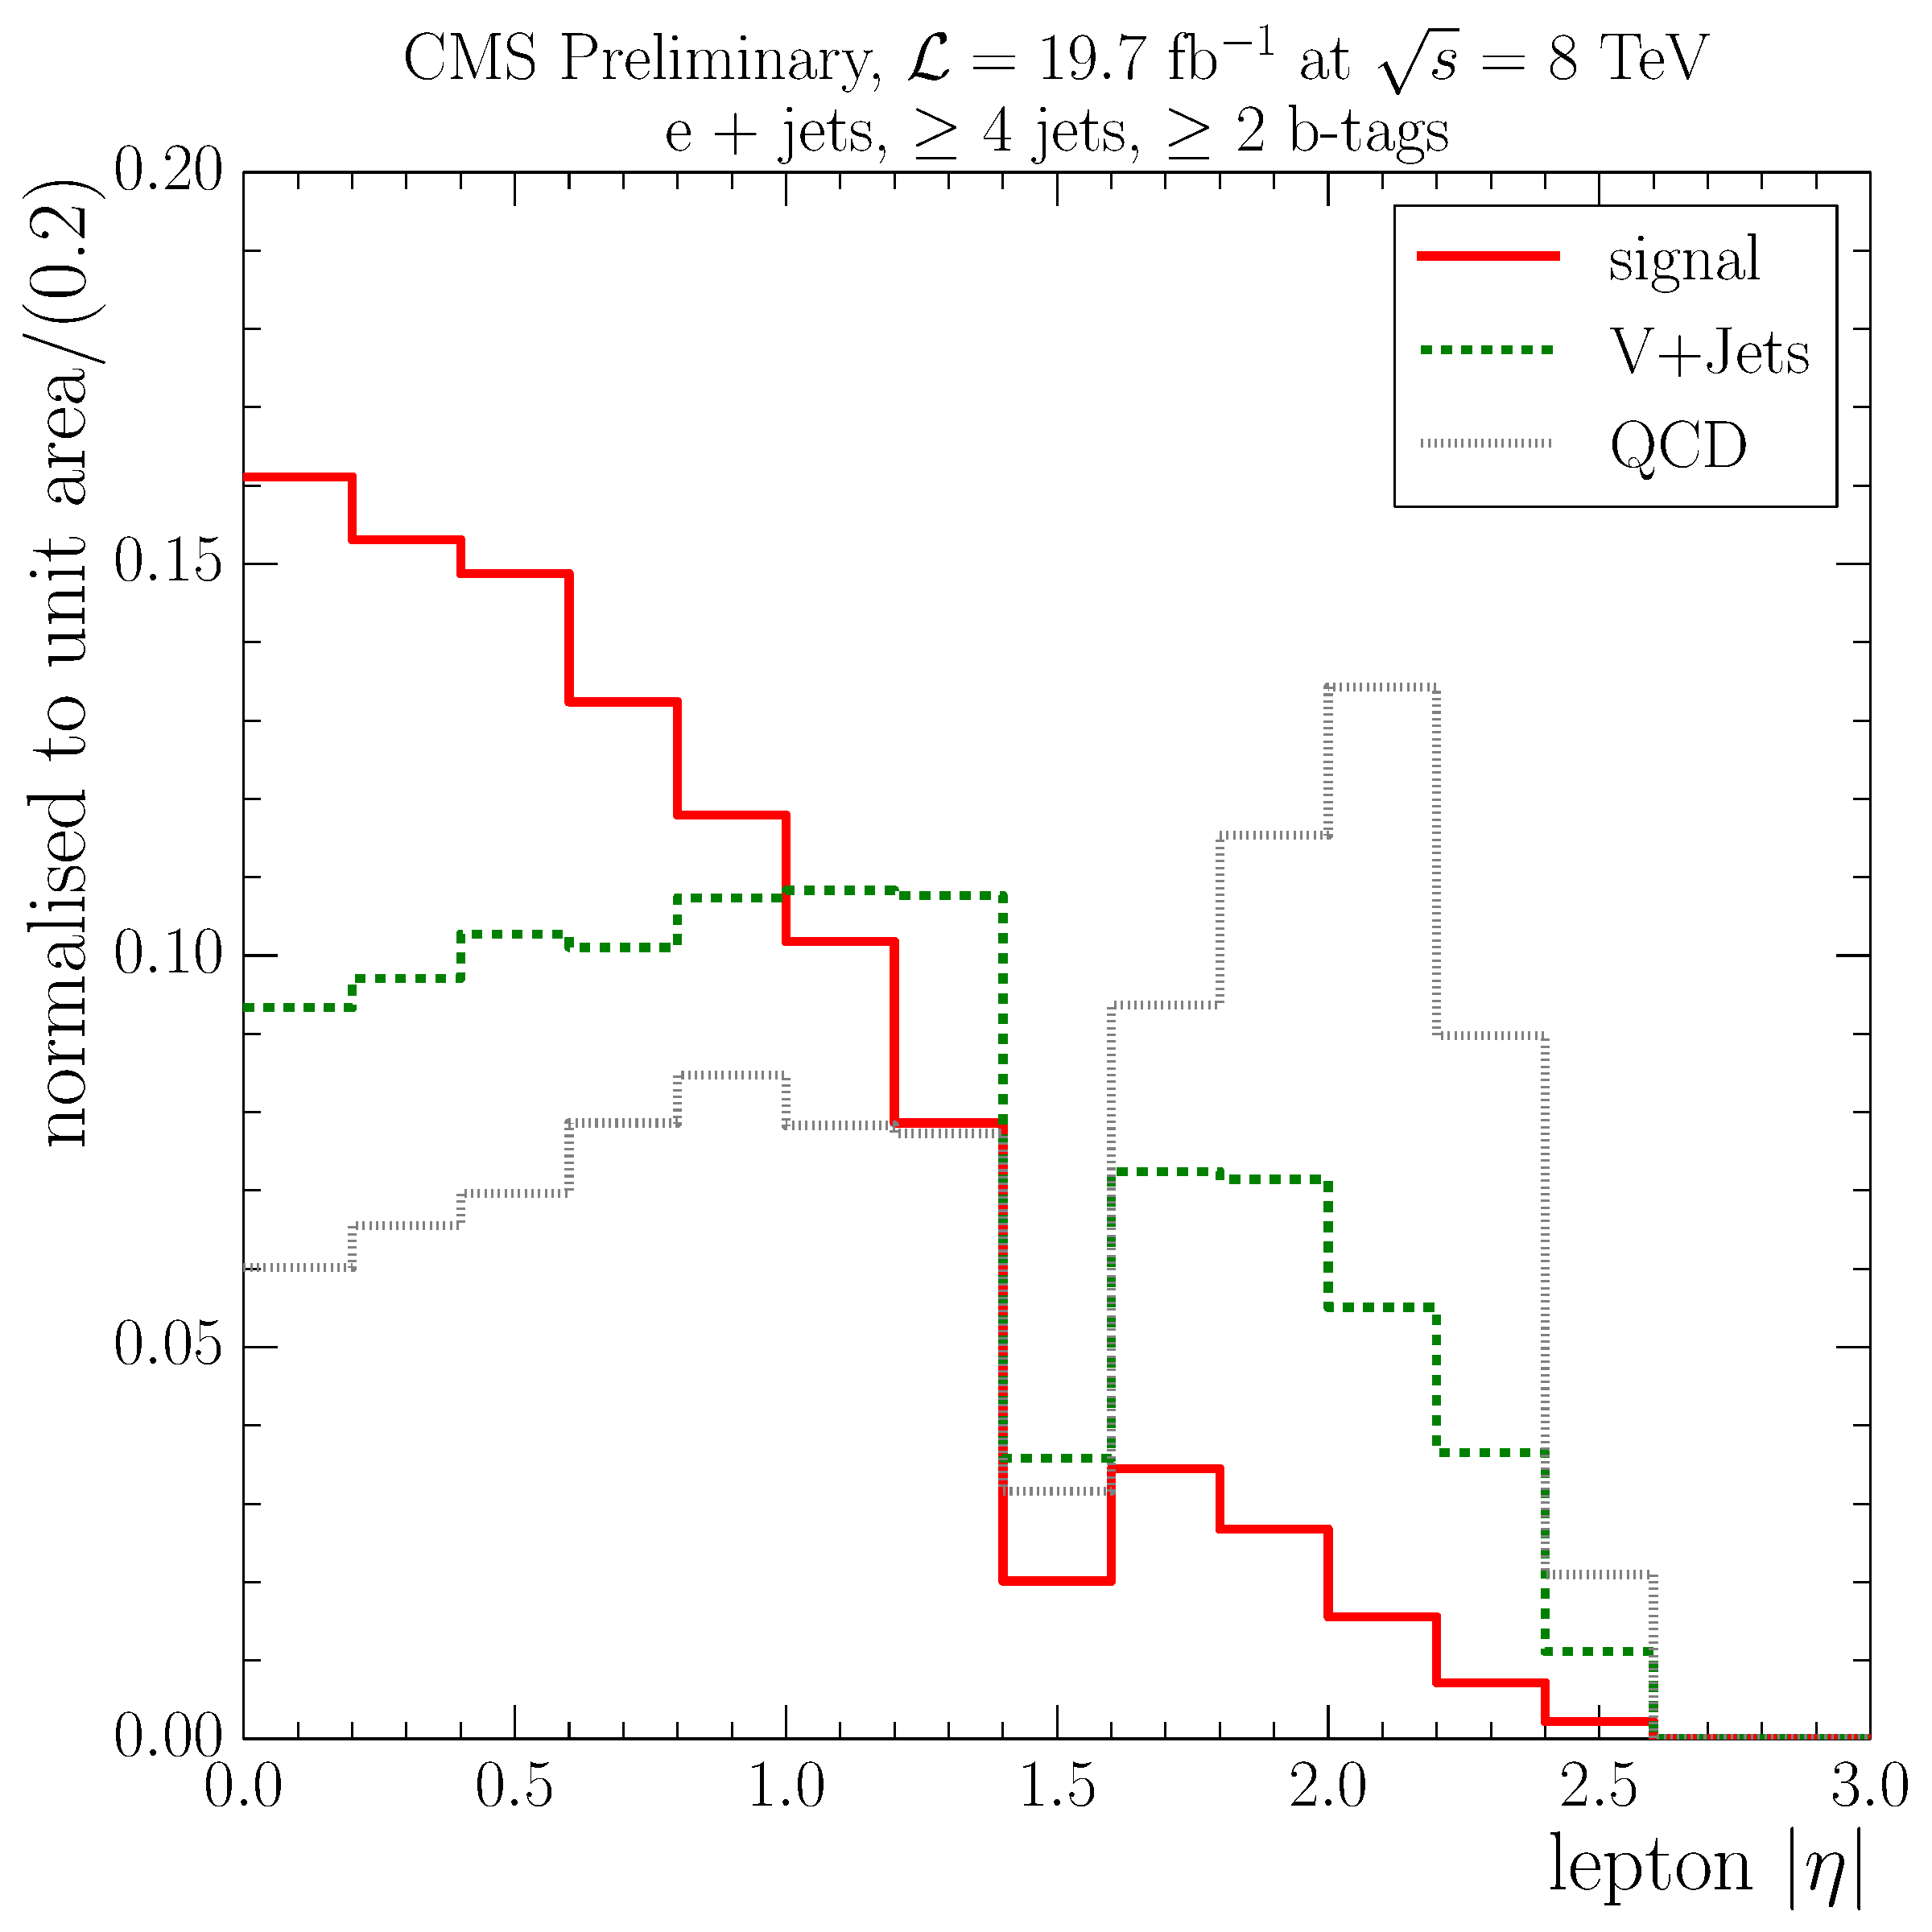
\includegraphics[width=0.3\textwidth]{measurement/ST/central/fit_templates/electron_templates_bin_500-580}}
    {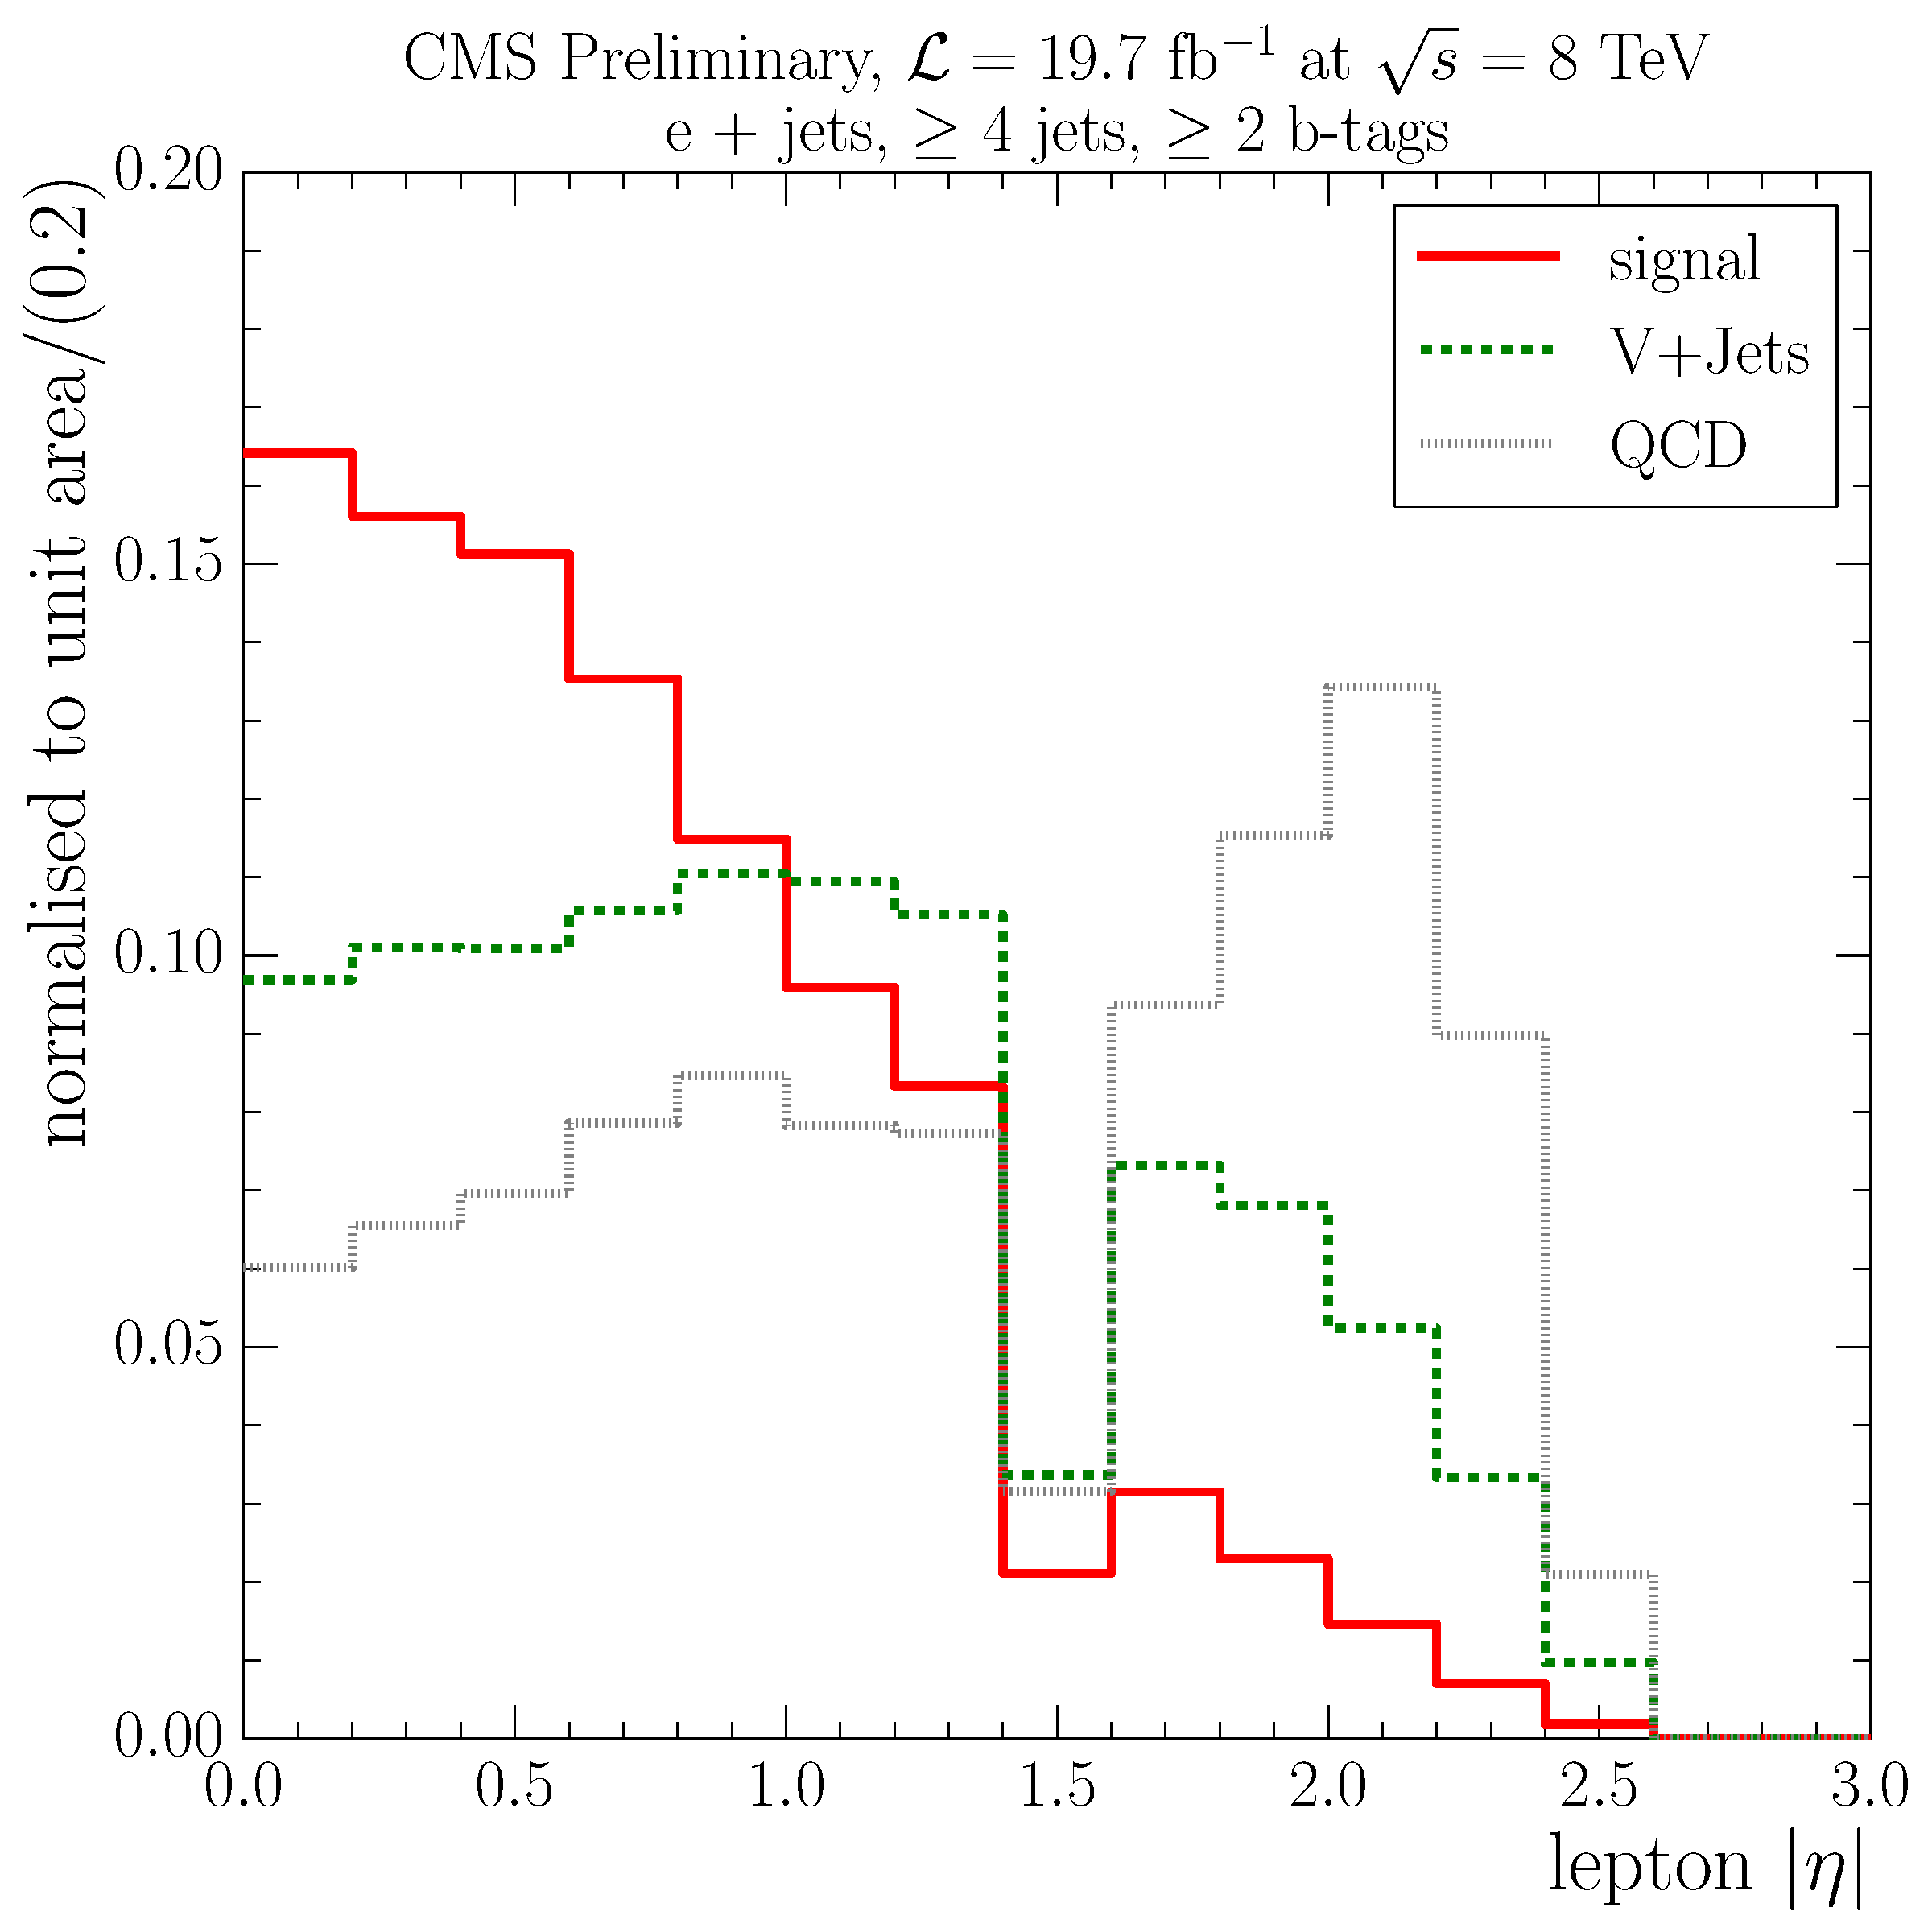
\includegraphics[width=0.3\textwidth]{measurement/ST/central/fit_templates/electron_templates_bin_580-700}}\\
    {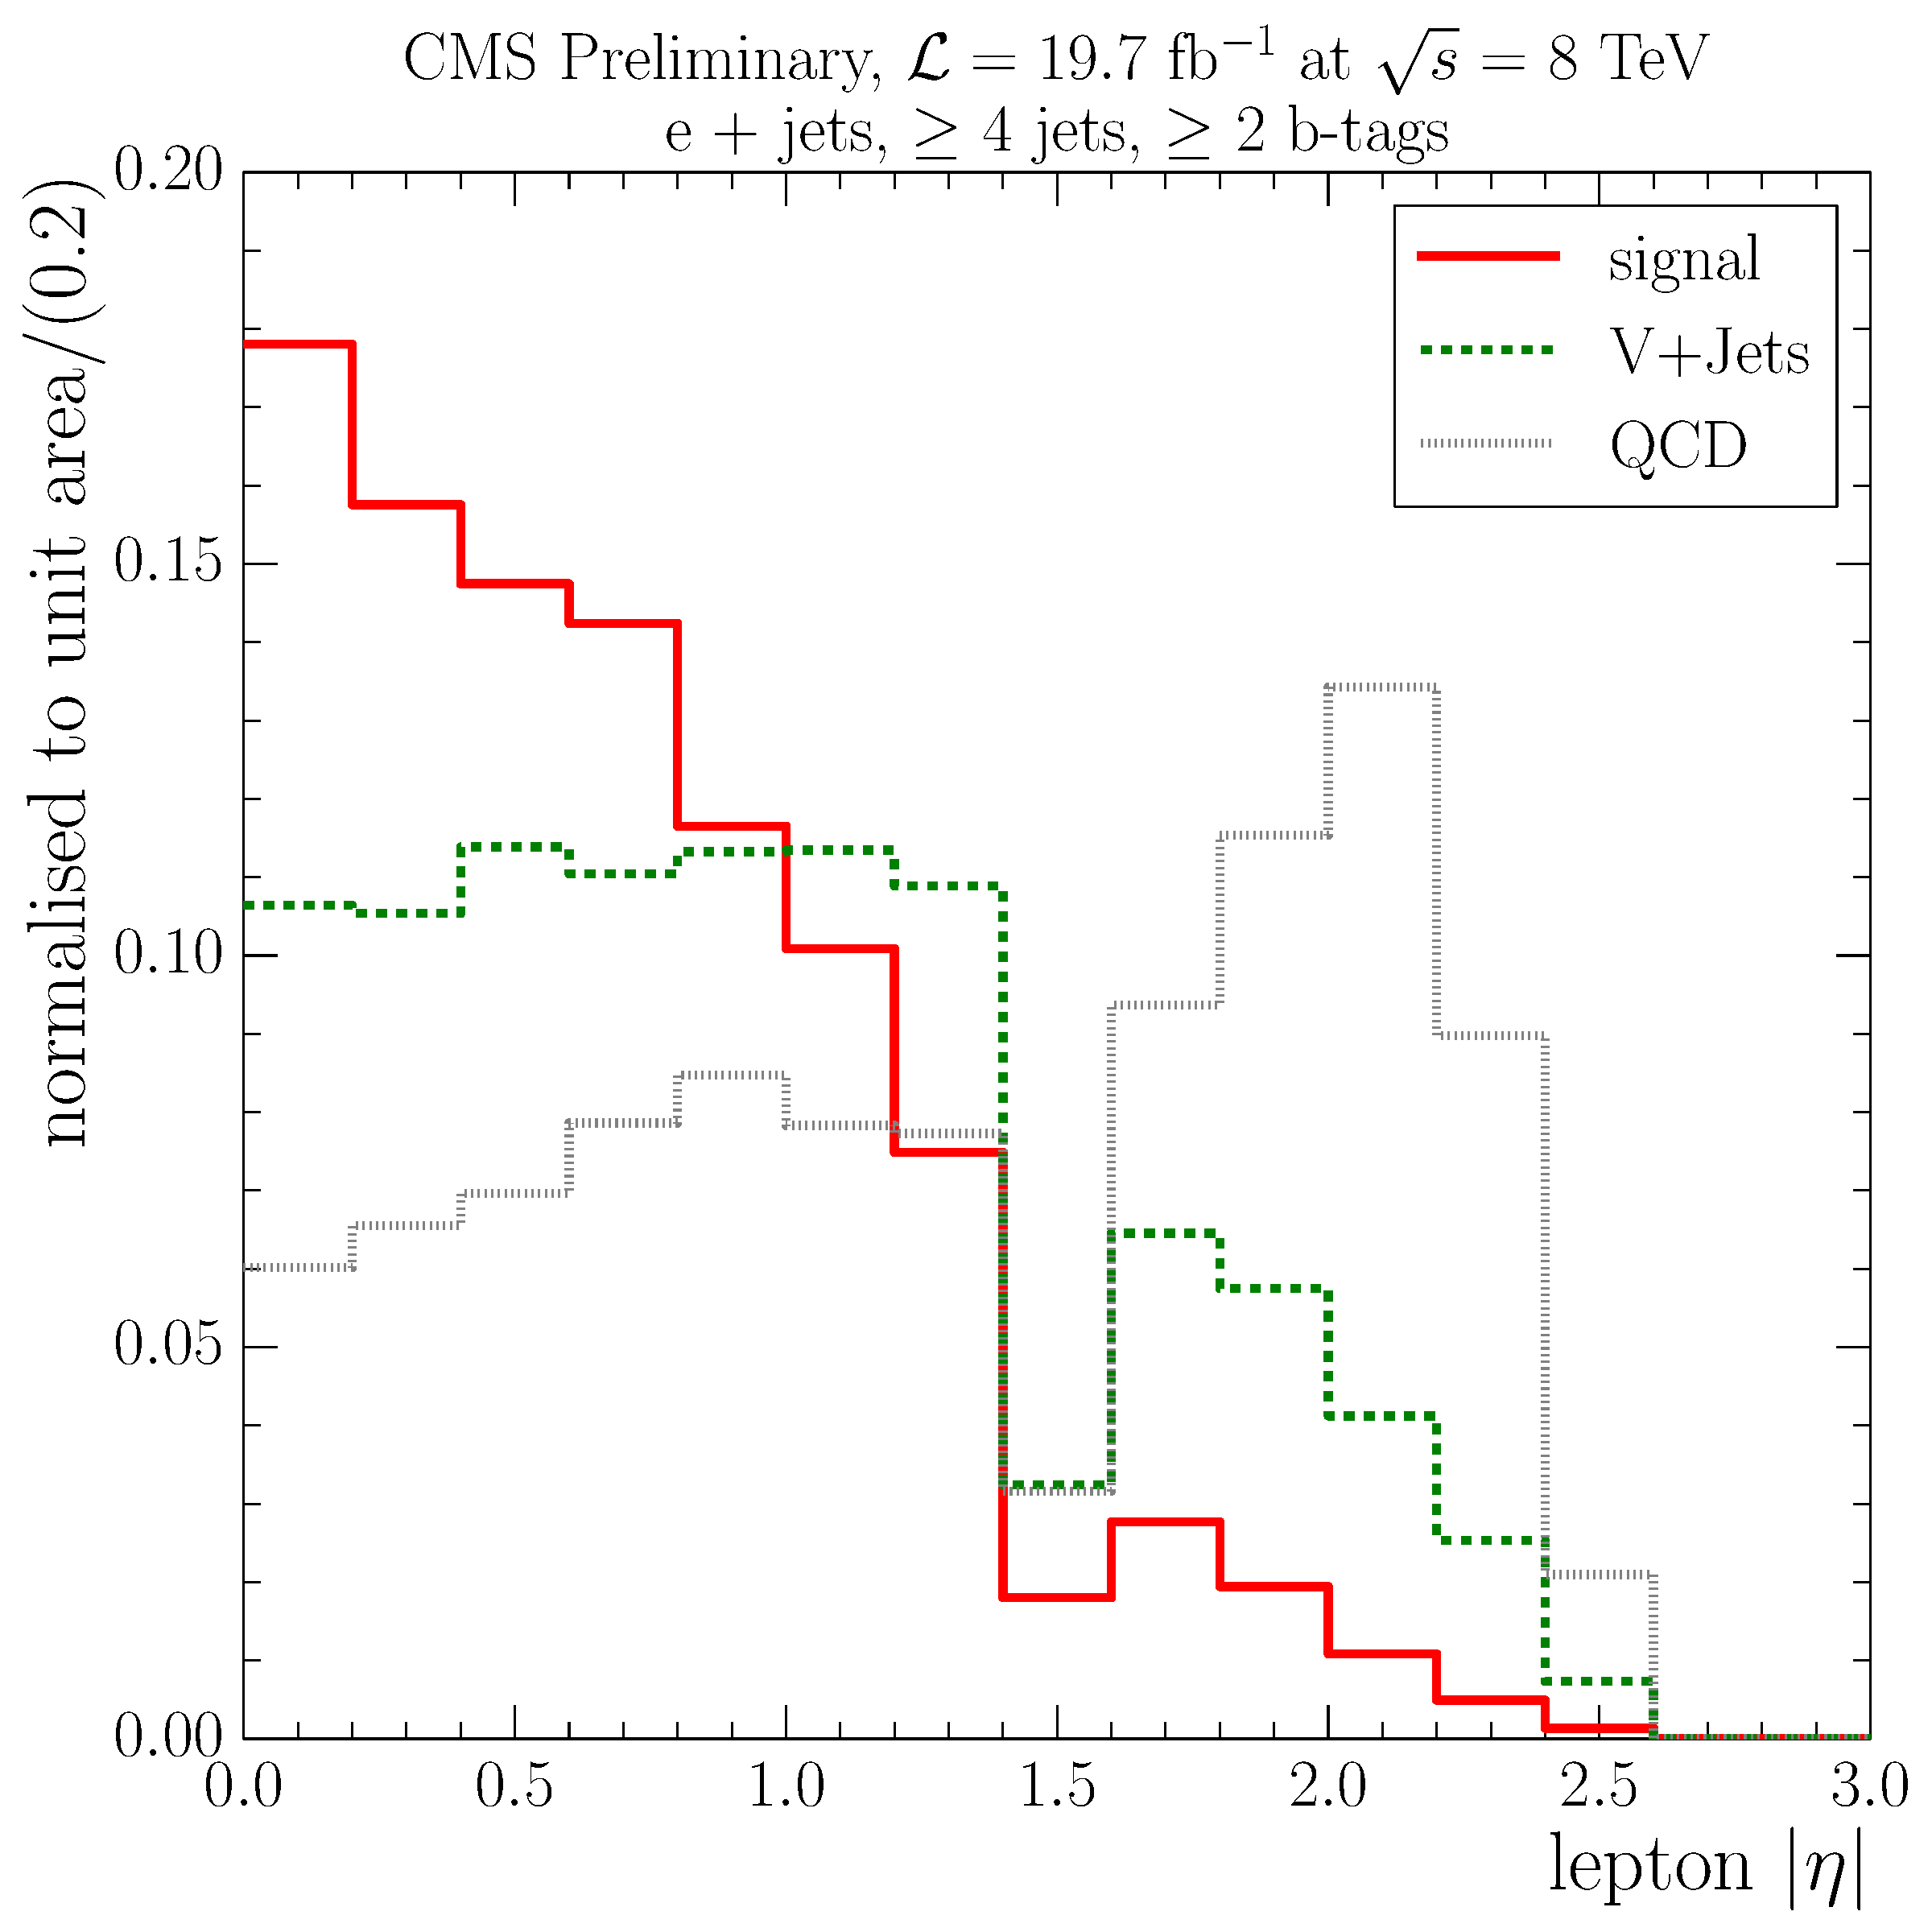
\includegraphics[width=0.3\textwidth]{measurement/ST/central/fit_templates/electron_templates_bin_700-inf}}
    \caption[Electron $\abs \eta$ templates for the fit in different bins of \ST]{Electron $\abs \eta$ templates for the
    fit in different bins of \ST, from top left to bottom: \SIrange{0}{350}{\GeV}, \SIrange{350}{400}{\GeV},
    \SIrange{400}{450}{\GeV}, \SIrange{450}{500}{\GeV}, \SIrange{500}{580}{\GeV}, \SIrange{580}{700}{\GeV} and $\geq
    \SI{700}{\GeV}$.}
    \label{fig:fit_tempaltes_ST_electron}
\end{figure}

\begin{figure}[!htbp]
  \centering
    {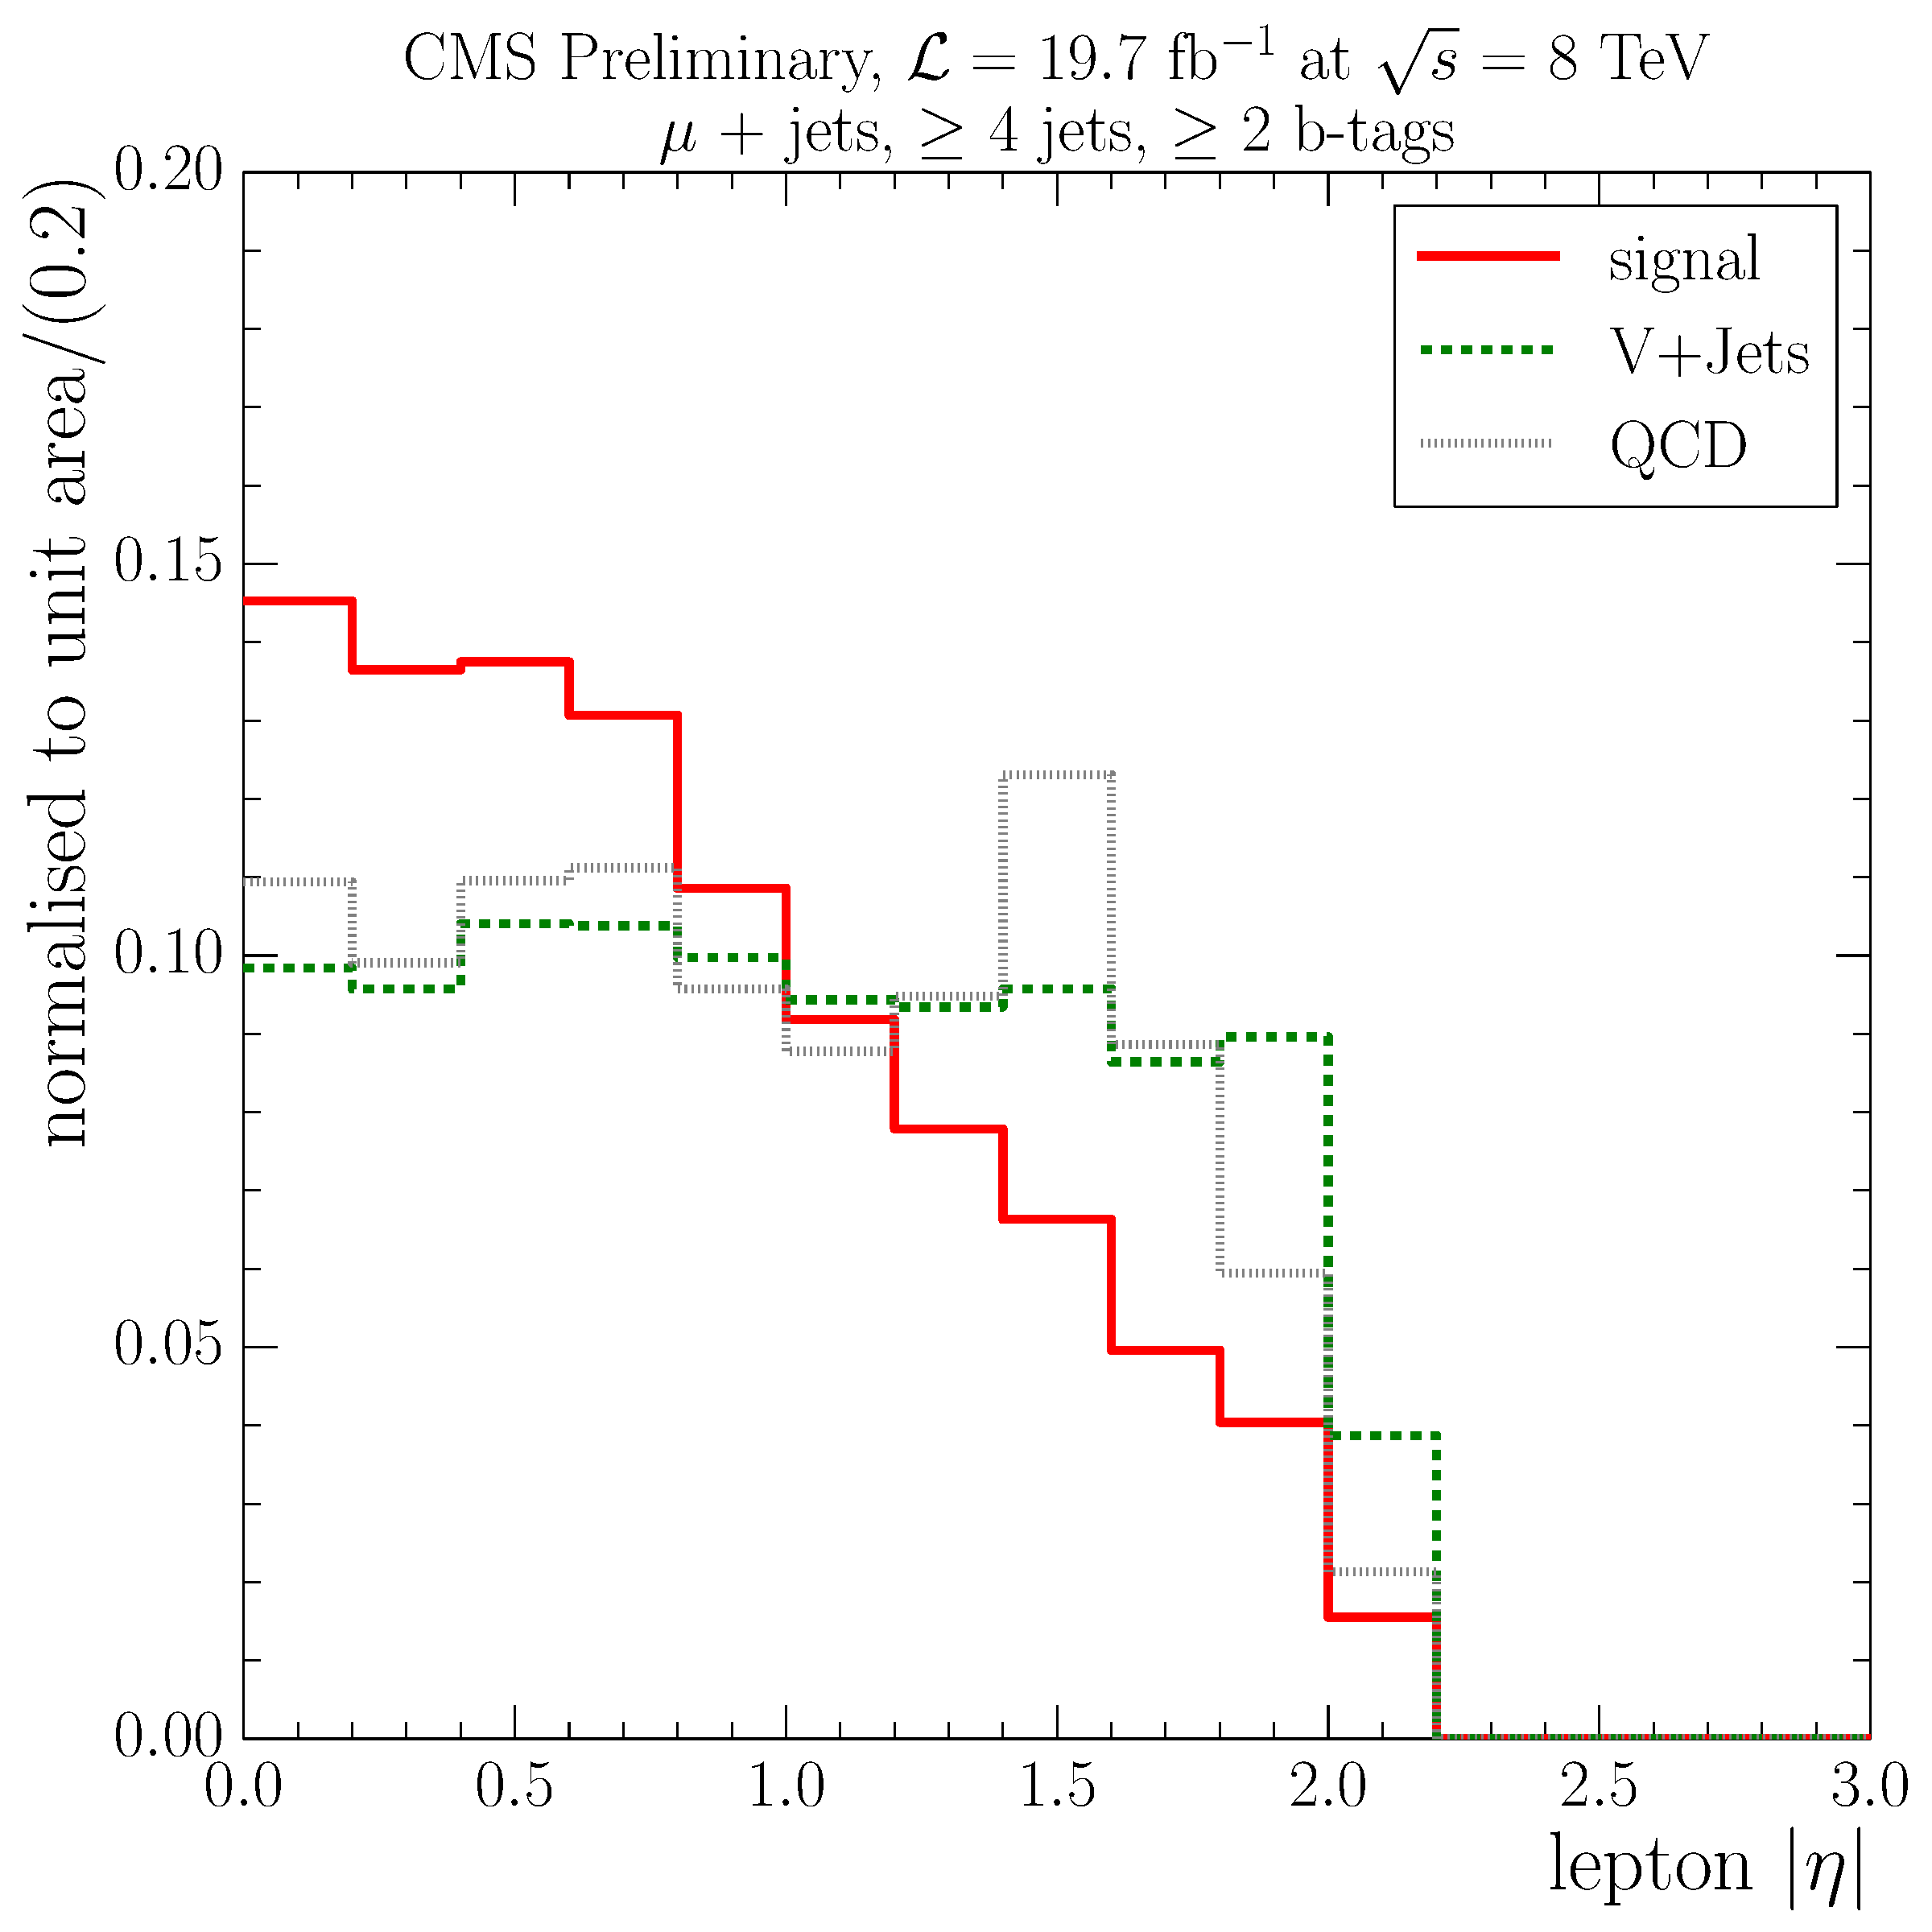
\includegraphics[width=0.3\textwidth]{measurement/ST/central/fit_templates/muon_templates_bin_0-350}}
    {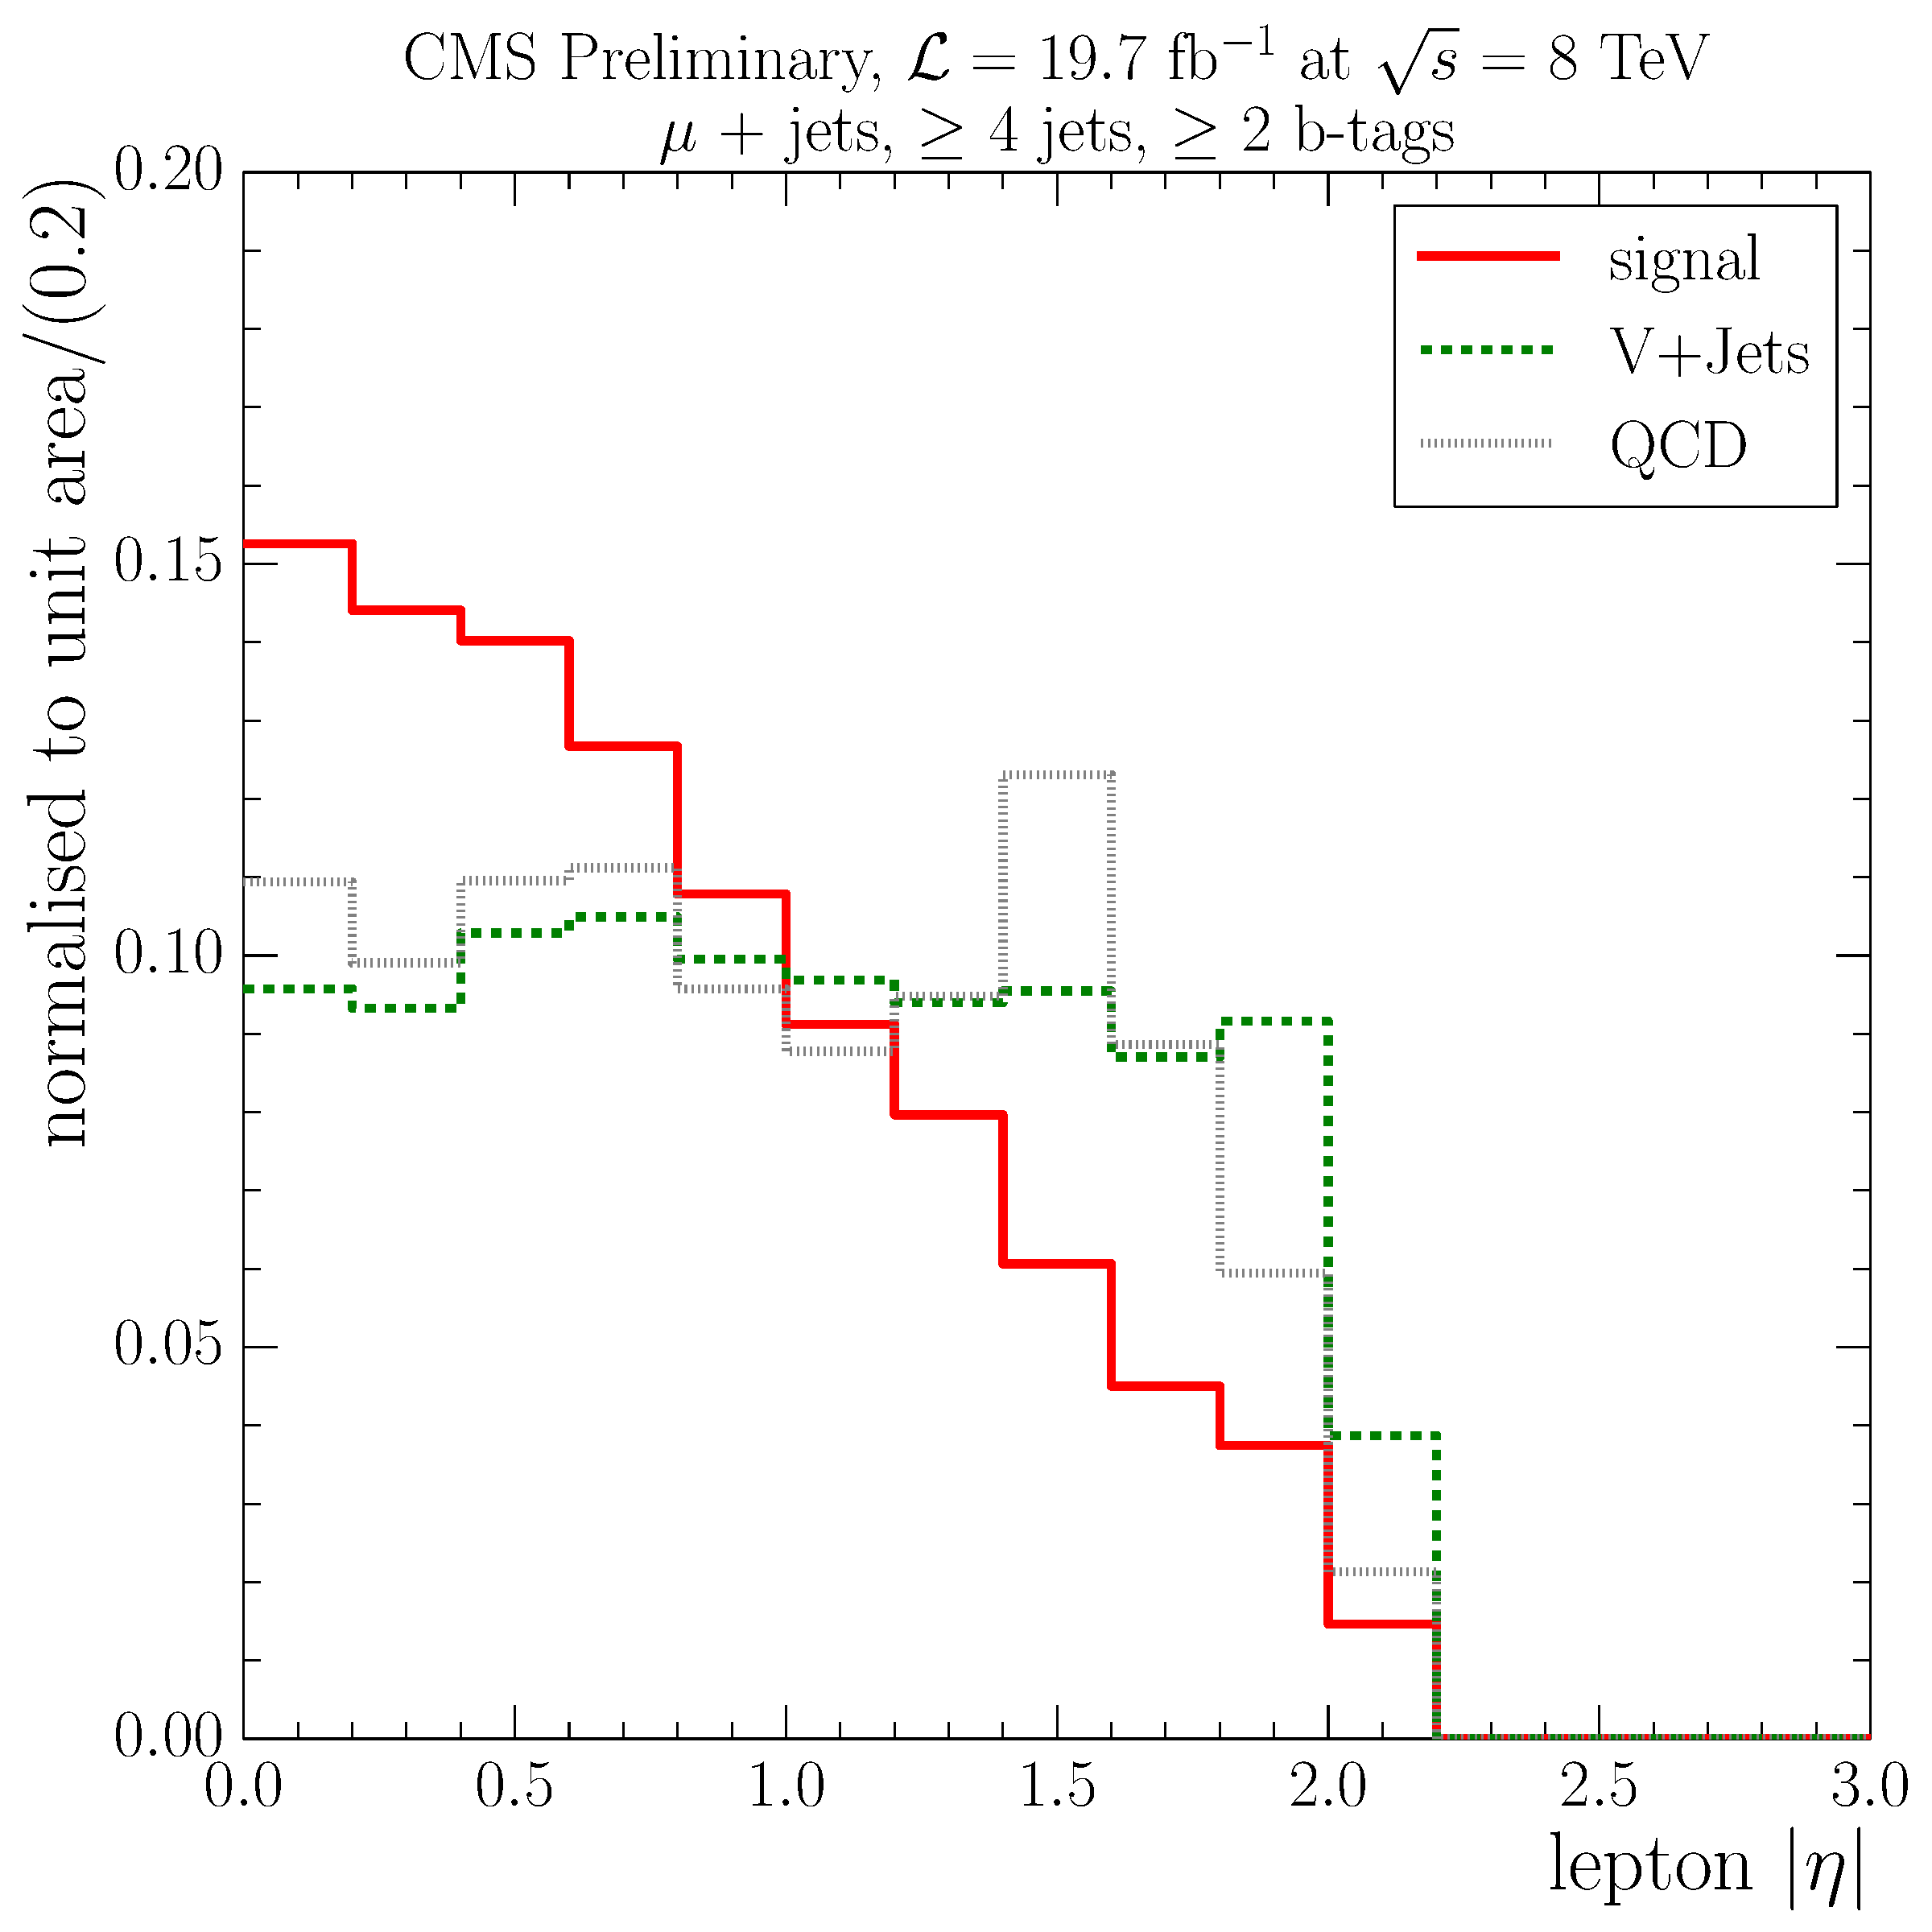
\includegraphics[width=0.3\textwidth]{measurement/ST/central/fit_templates/muon_templates_bin_350-400}}
    {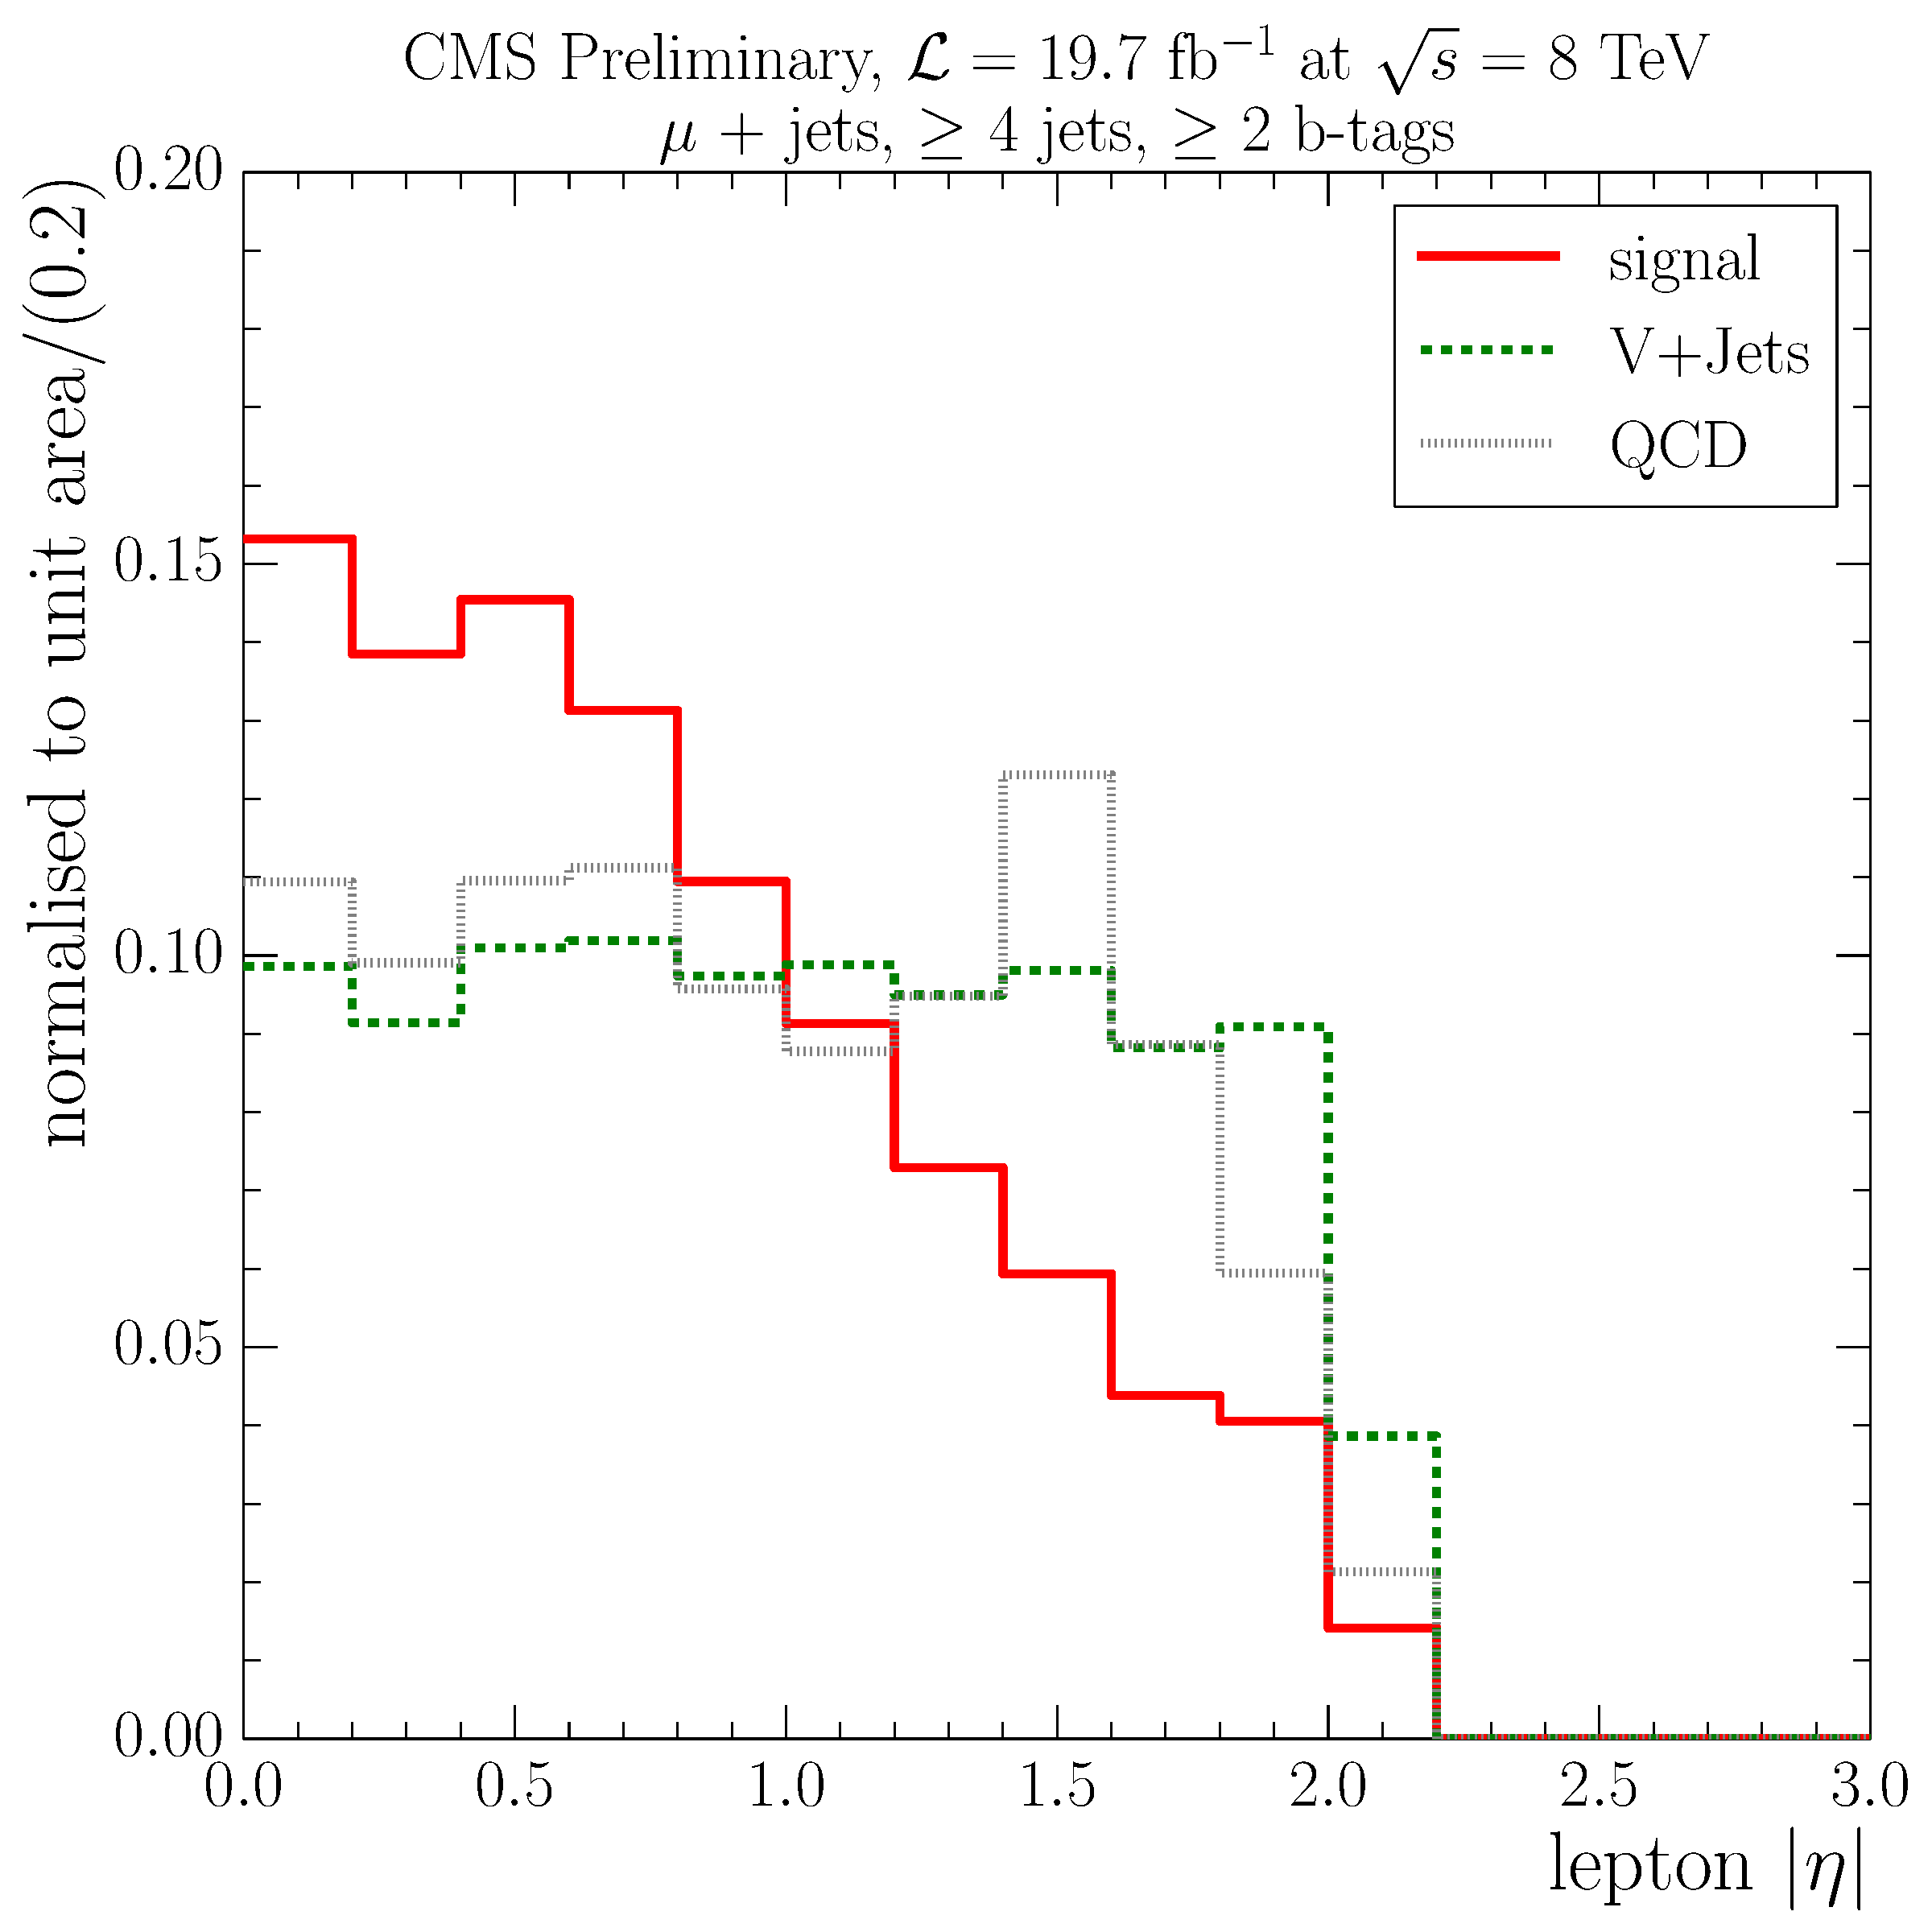
\includegraphics[width=0.3\textwidth]{measurement/ST/central/fit_templates/muon_templates_bin_400-450}}\\
    {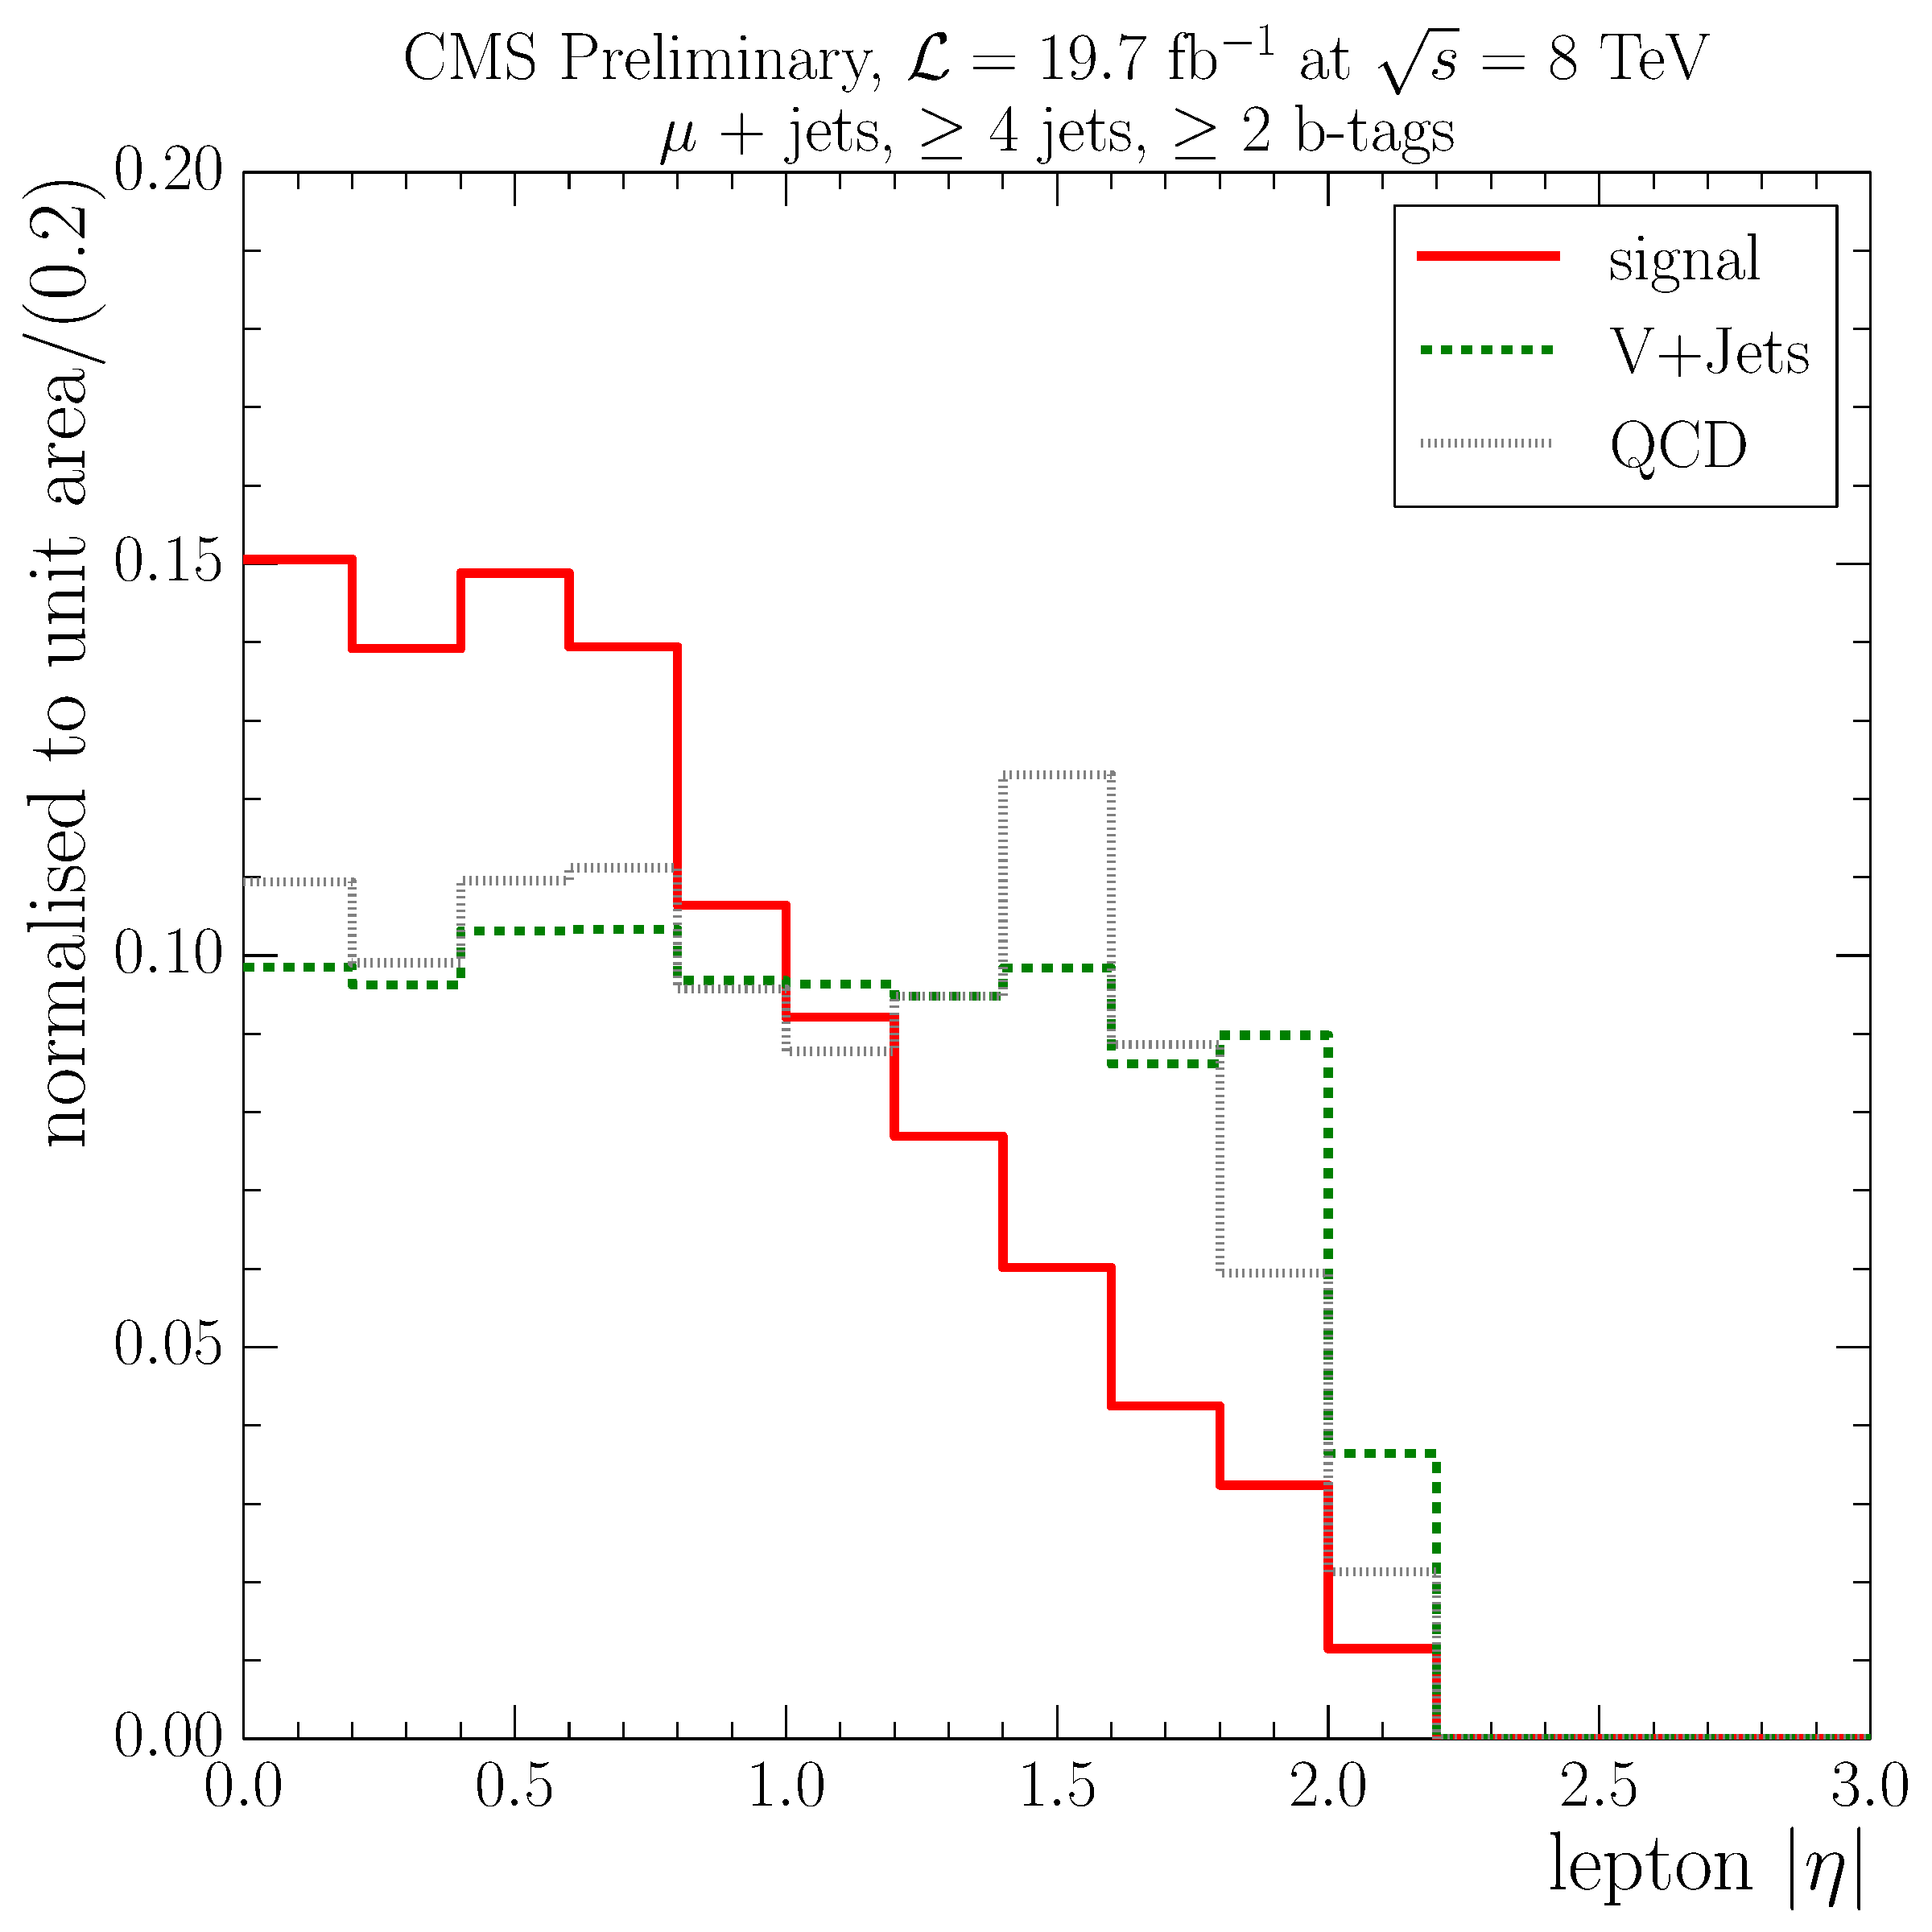
\includegraphics[width=0.3\textwidth]{measurement/ST/central/fit_templates/muon_templates_bin_450-500}}
    {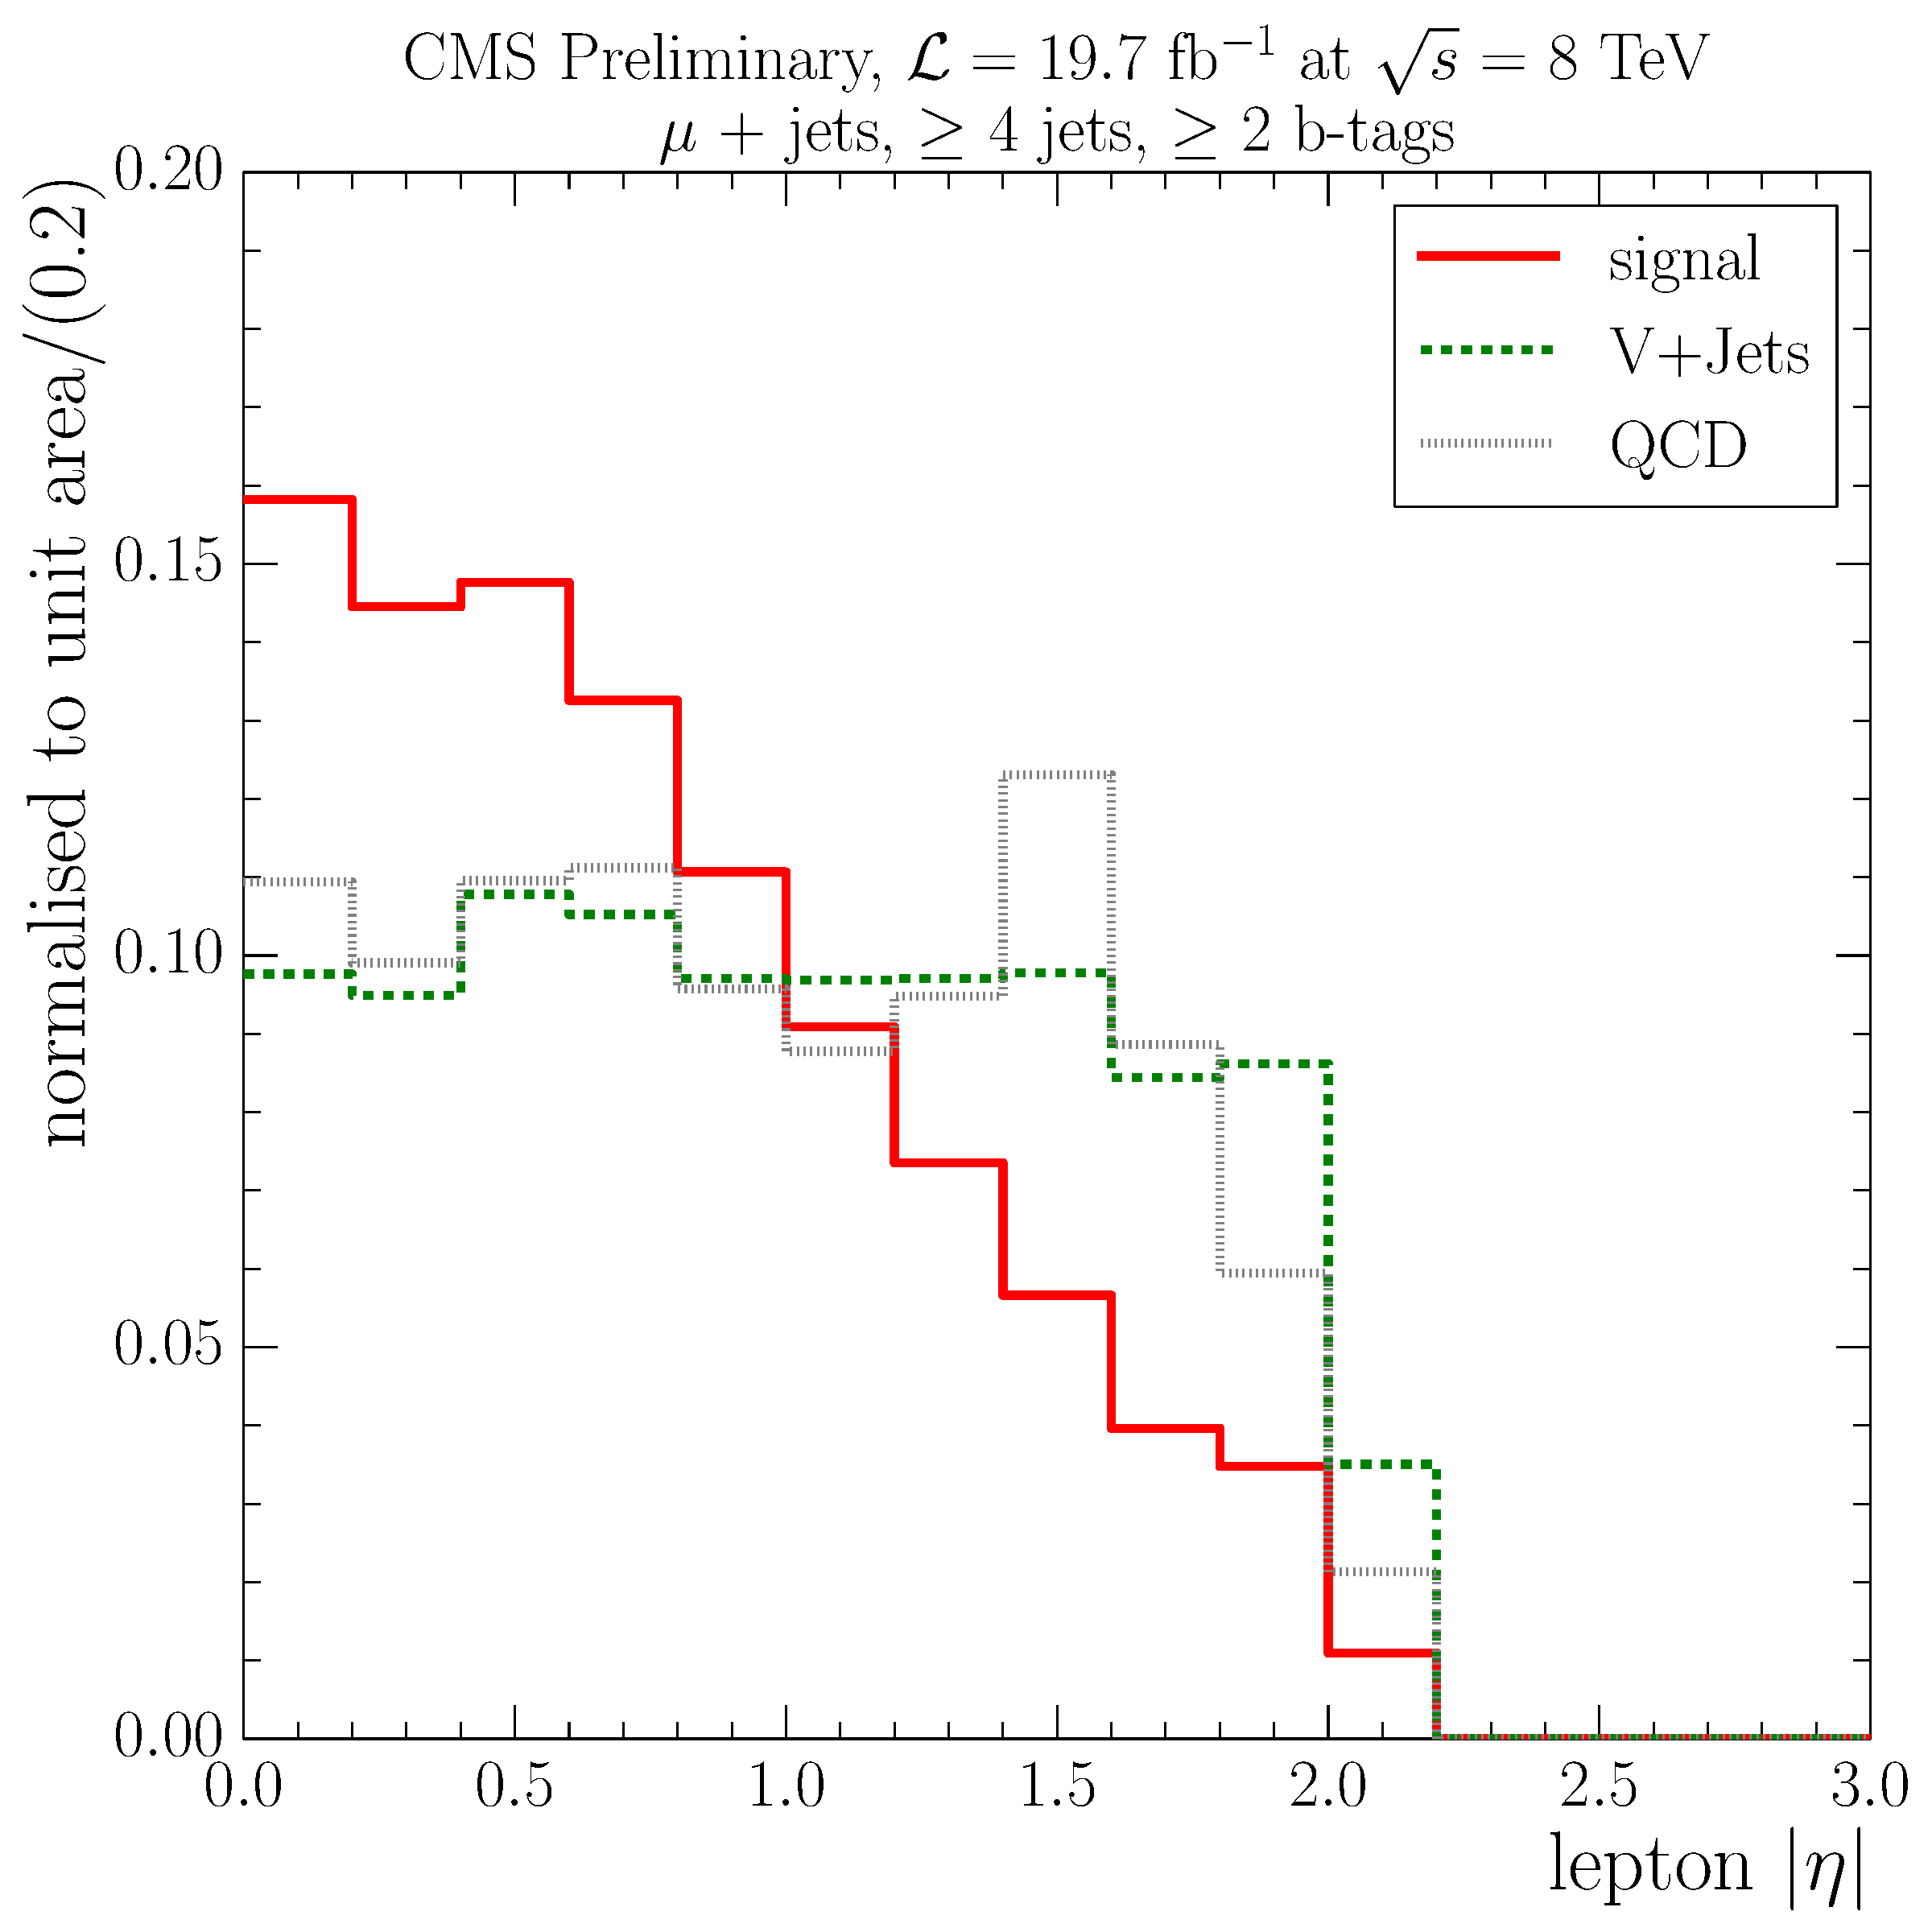
\includegraphics[width=0.3\textwidth]{measurement/ST/central/fit_templates/muon_templates_bin_500-580}}
    {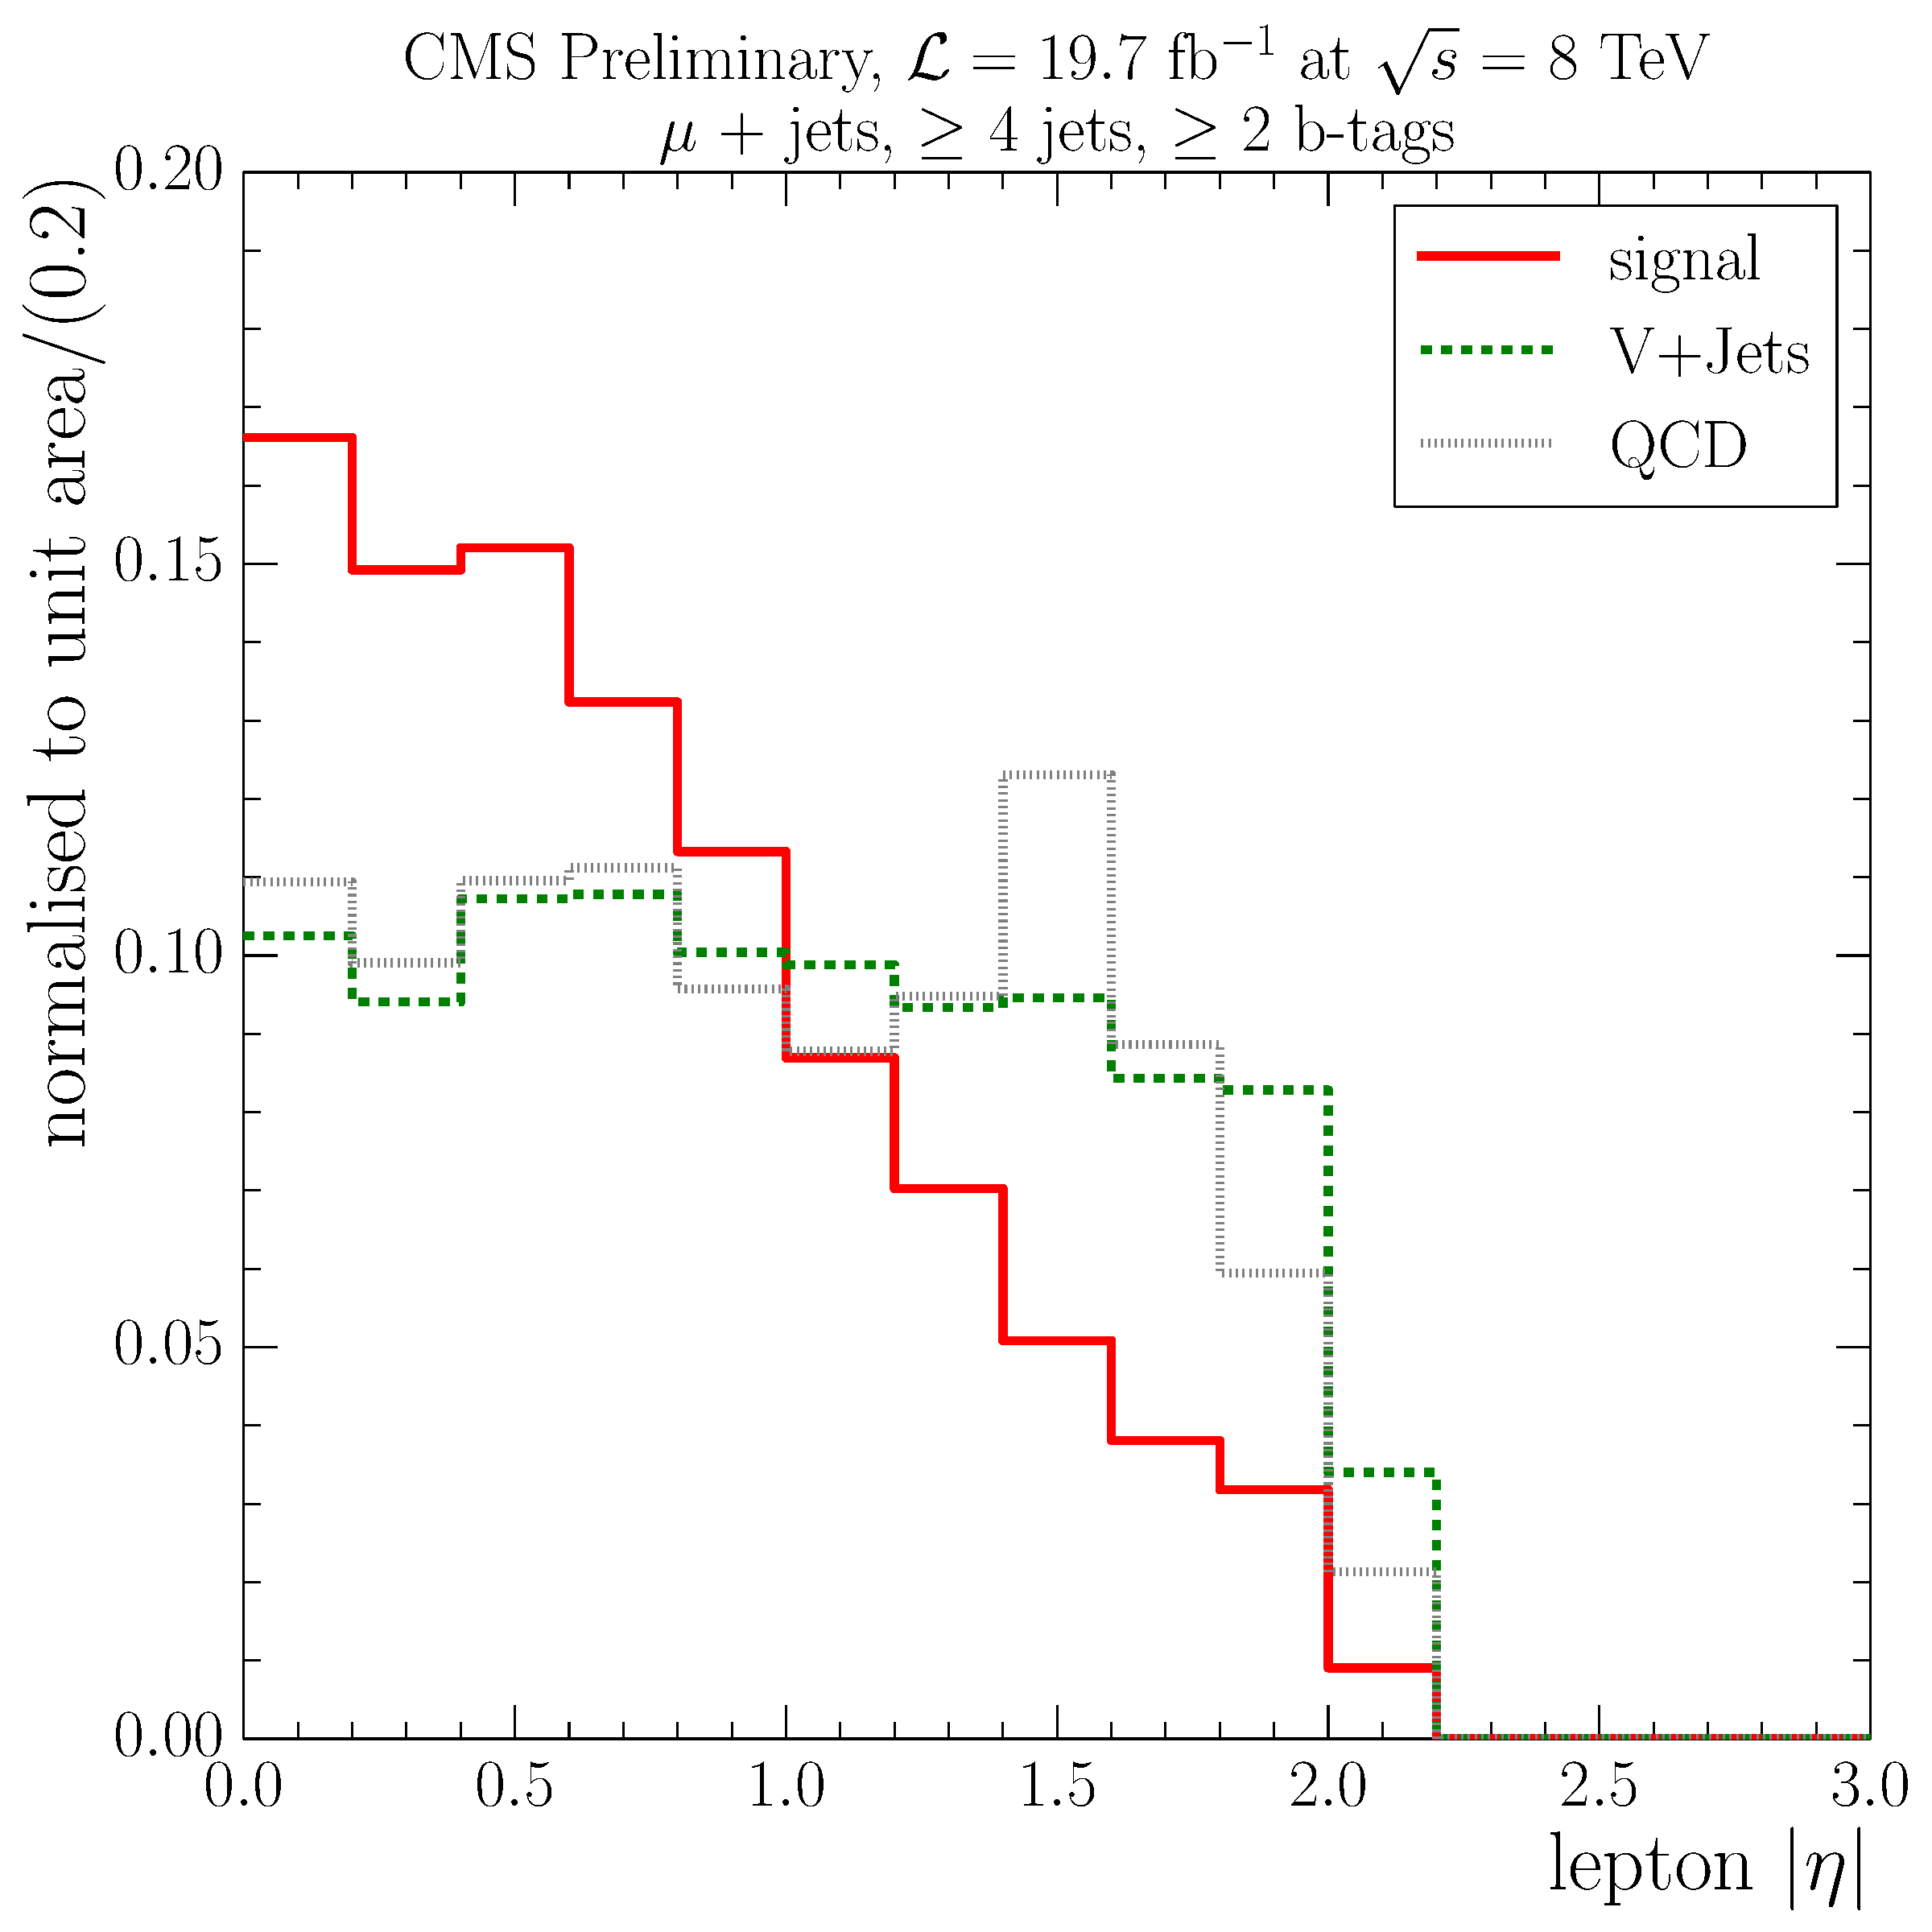
\includegraphics[width=0.3\textwidth]{measurement/ST/central/fit_templates/muon_templates_bin_580-700}}\\
    {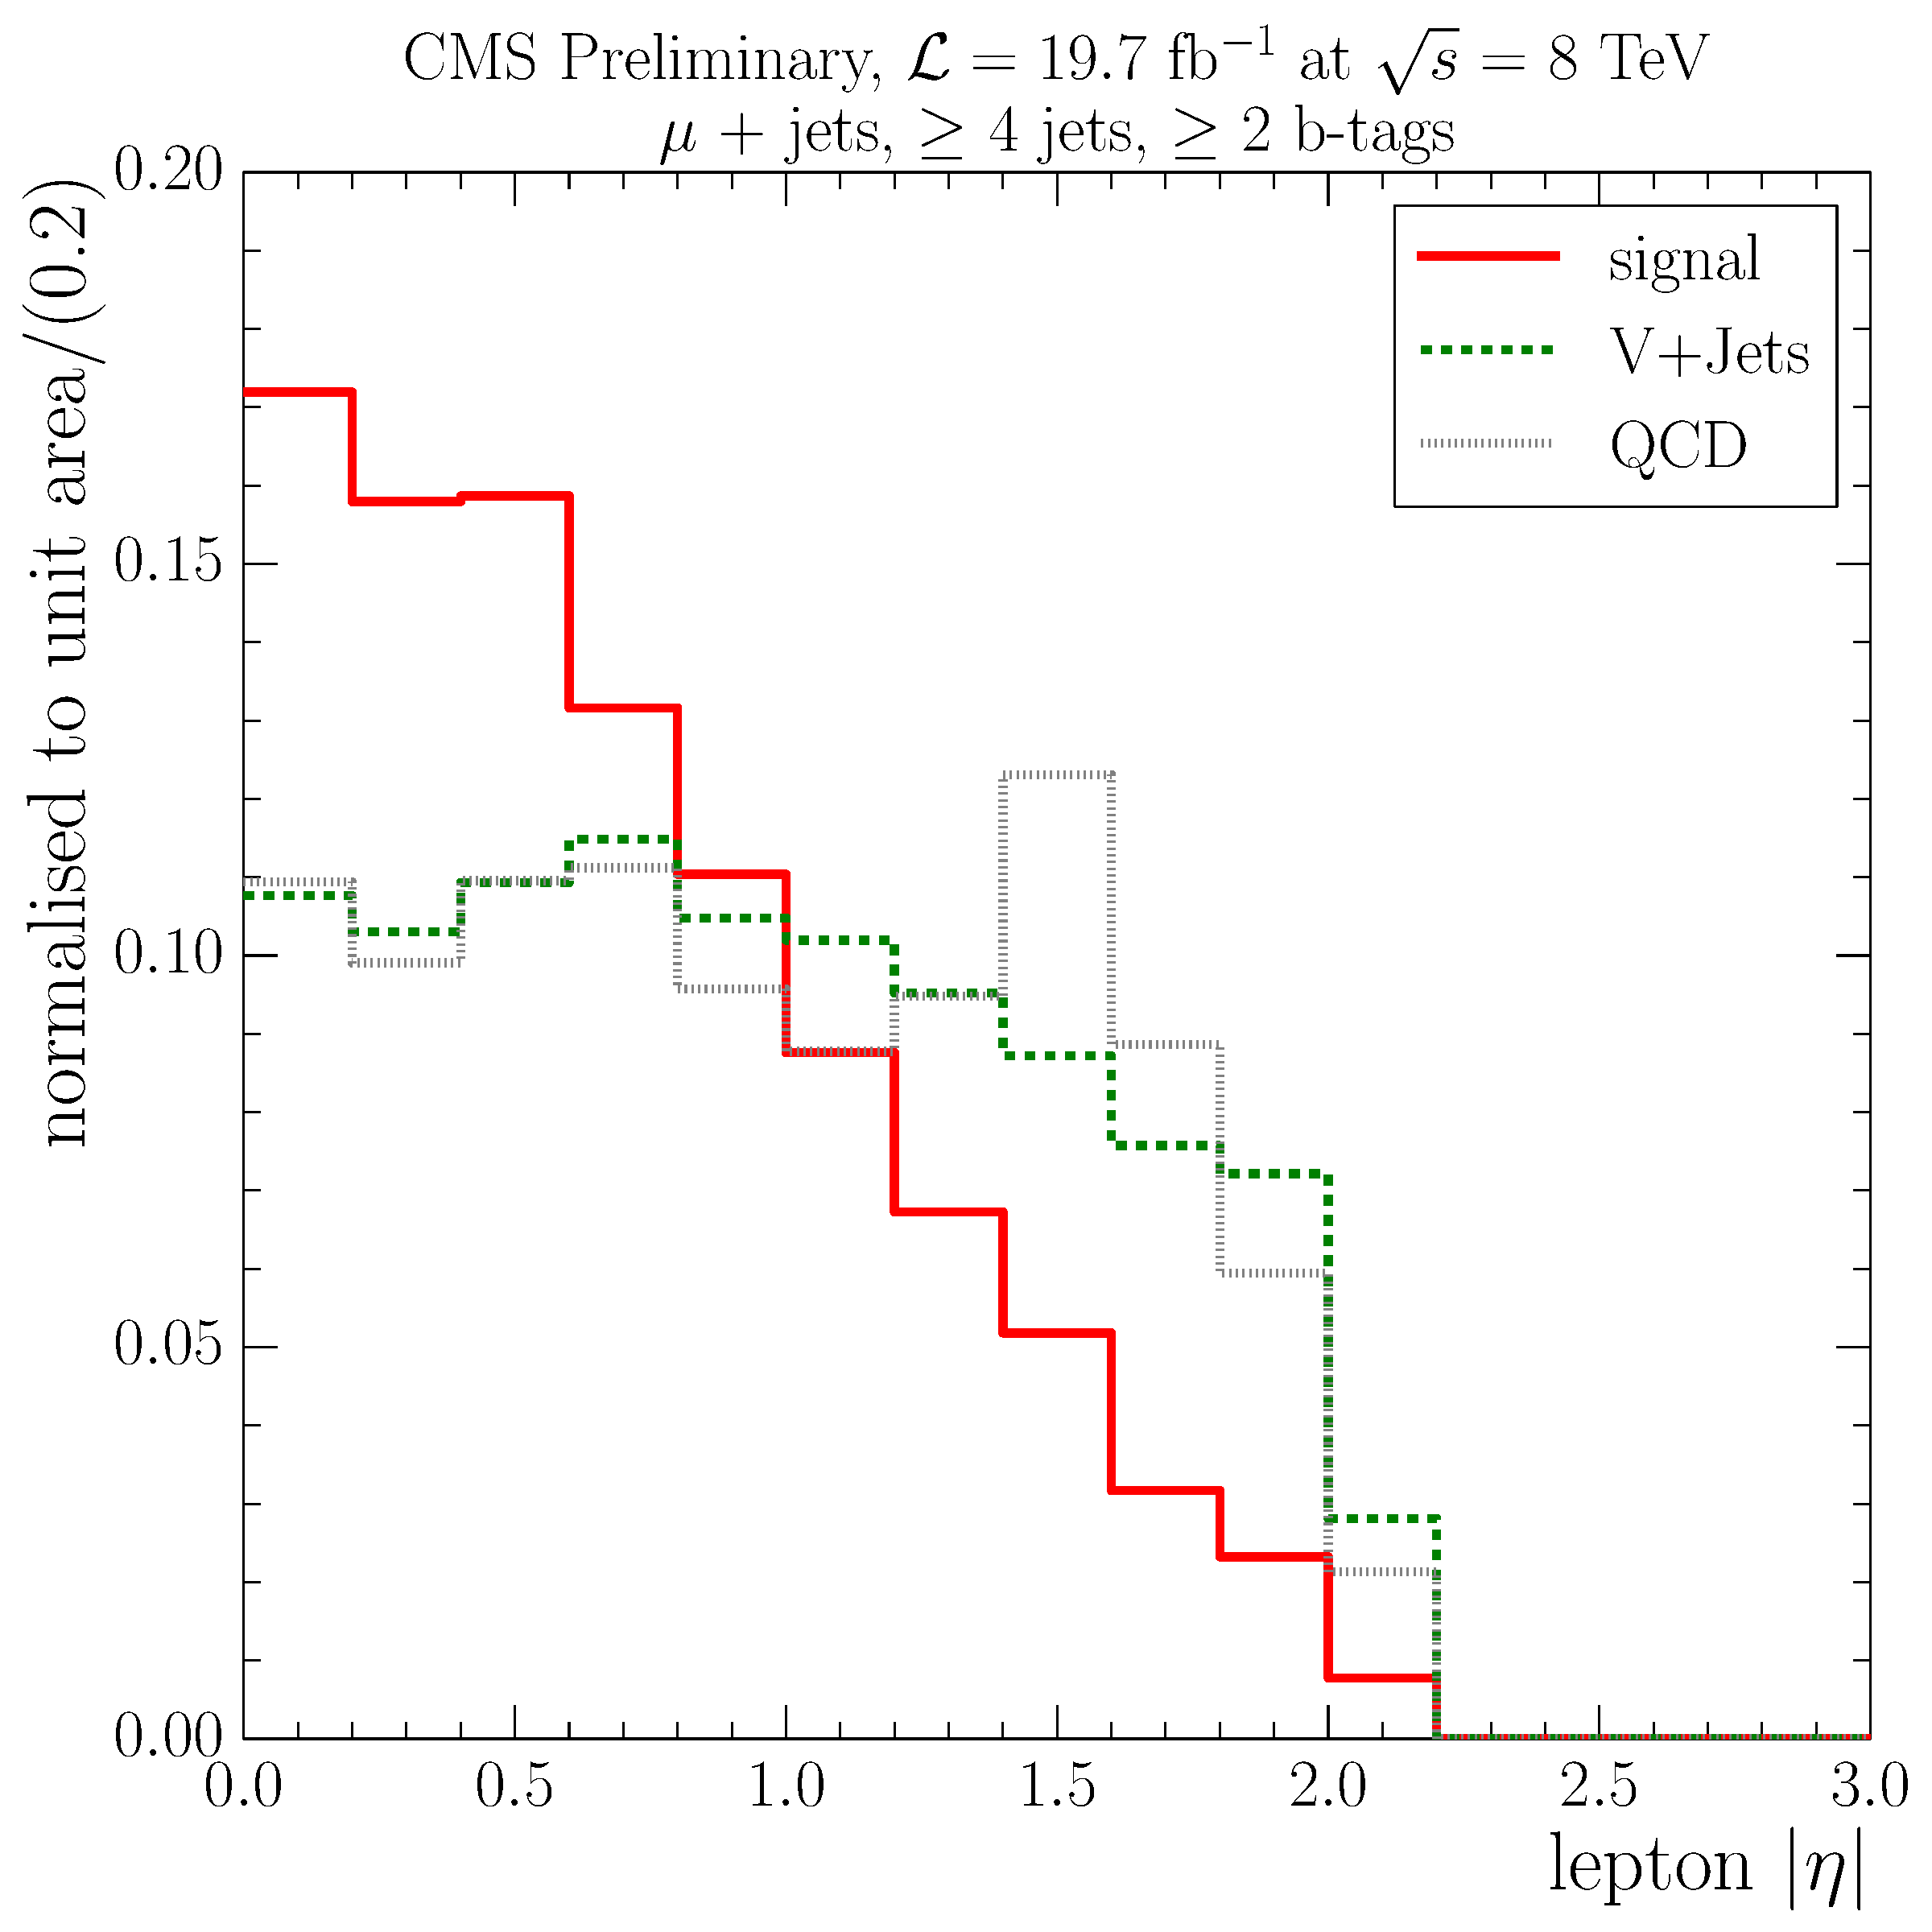
\includegraphics[width=0.3\textwidth]{measurement/ST/central/fit_templates/muon_templates_bin_700-inf}}
    \caption[Muon $\abs \eta$ templates for the fit in different bins of \ST]{Muon $\abs \eta$ templates for the fit in
    different bins of \ST, from top left to bottom: \SIrange{0}{350}{\GeV}, \SIrange{350}{400}{\GeV},
    \SIrange{400}{450}{\GeV}, \SIrange{450}{500}{\GeV}, \SIrange{500}{580}{\GeV}, \SIrange{580}{700}{\GeV} and $\geq
    \SI{700}{\GeV}$.}
    \label{fig:fit_templates_ST_muon}
\end{figure}

\newpage
\section*{\WPT variable}

\begin{figure}[!htbp]
  \centering
    \vspace*{-0.5cm}
    \hspace*{\fill}
    {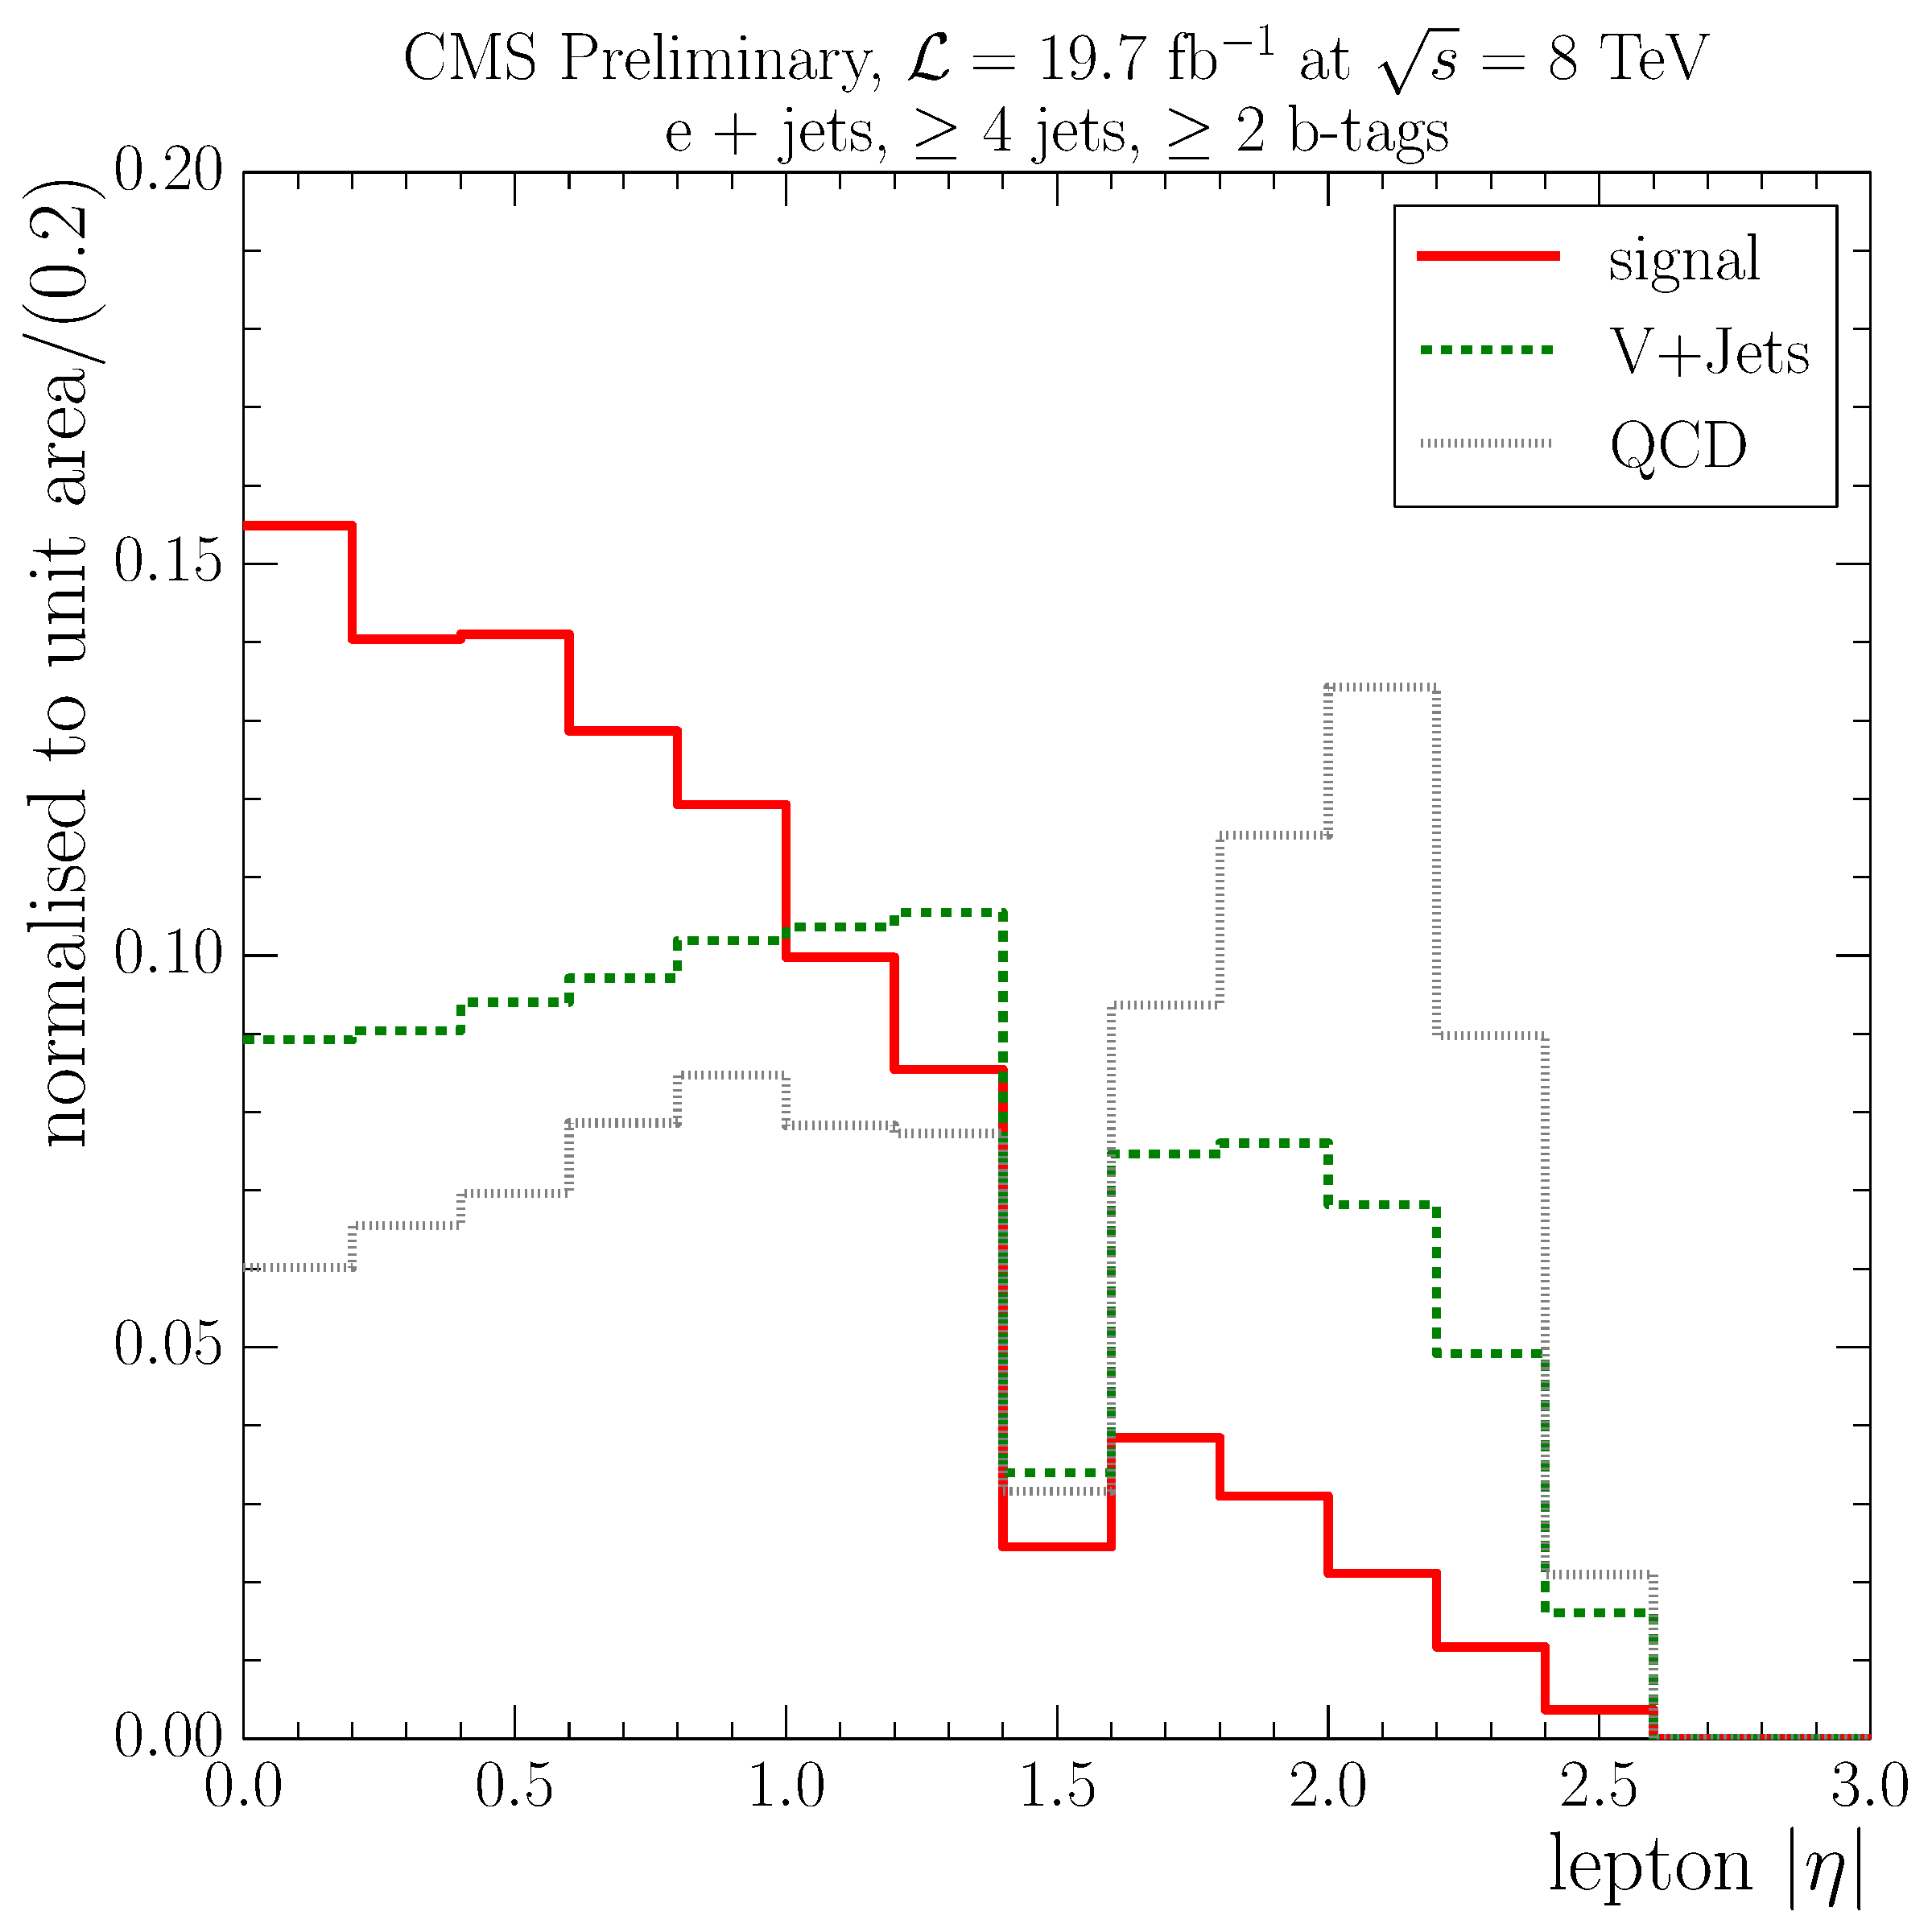
\includegraphics[width=0.39\textwidth]{measurement/WPT/central/fit_templates/electron_templates_bin_0-40}}\hfill
    {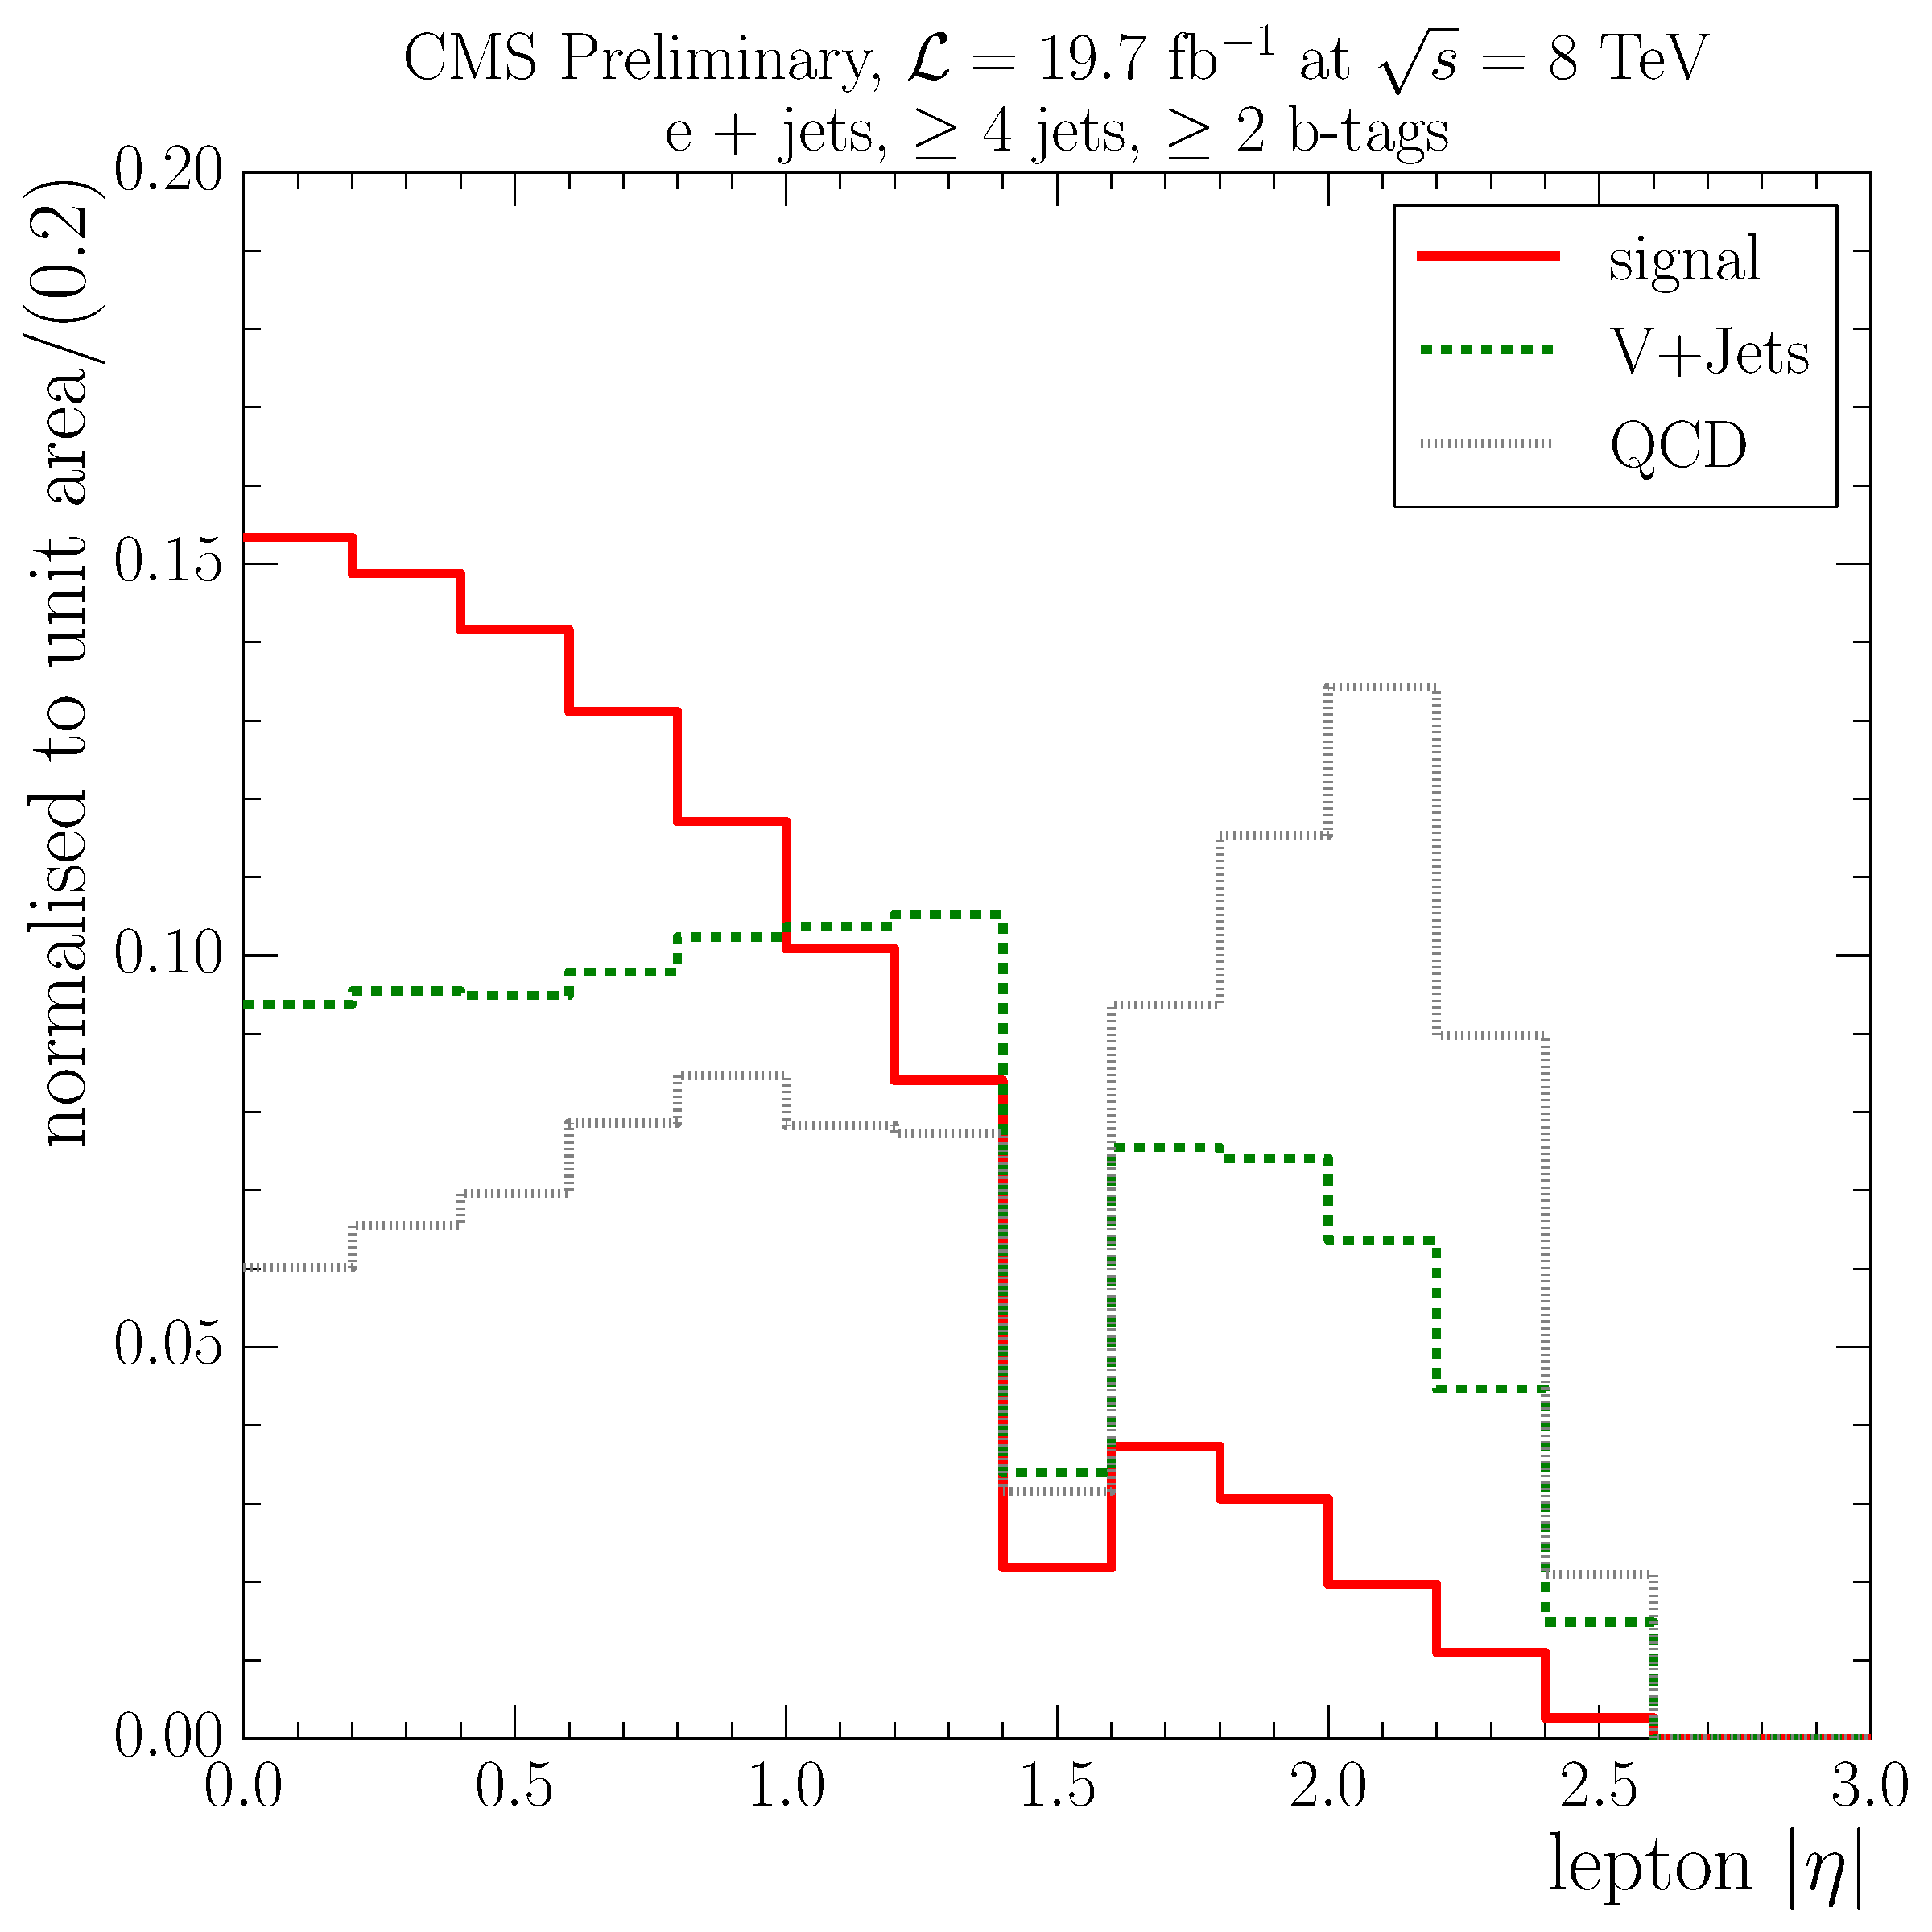
\includegraphics[width=0.39\textwidth]{measurement/WPT/central/fit_templates/electron_templates_bin_40-70}}
    \hspace*{\fill} \\
    \hspace*{\fill}
    {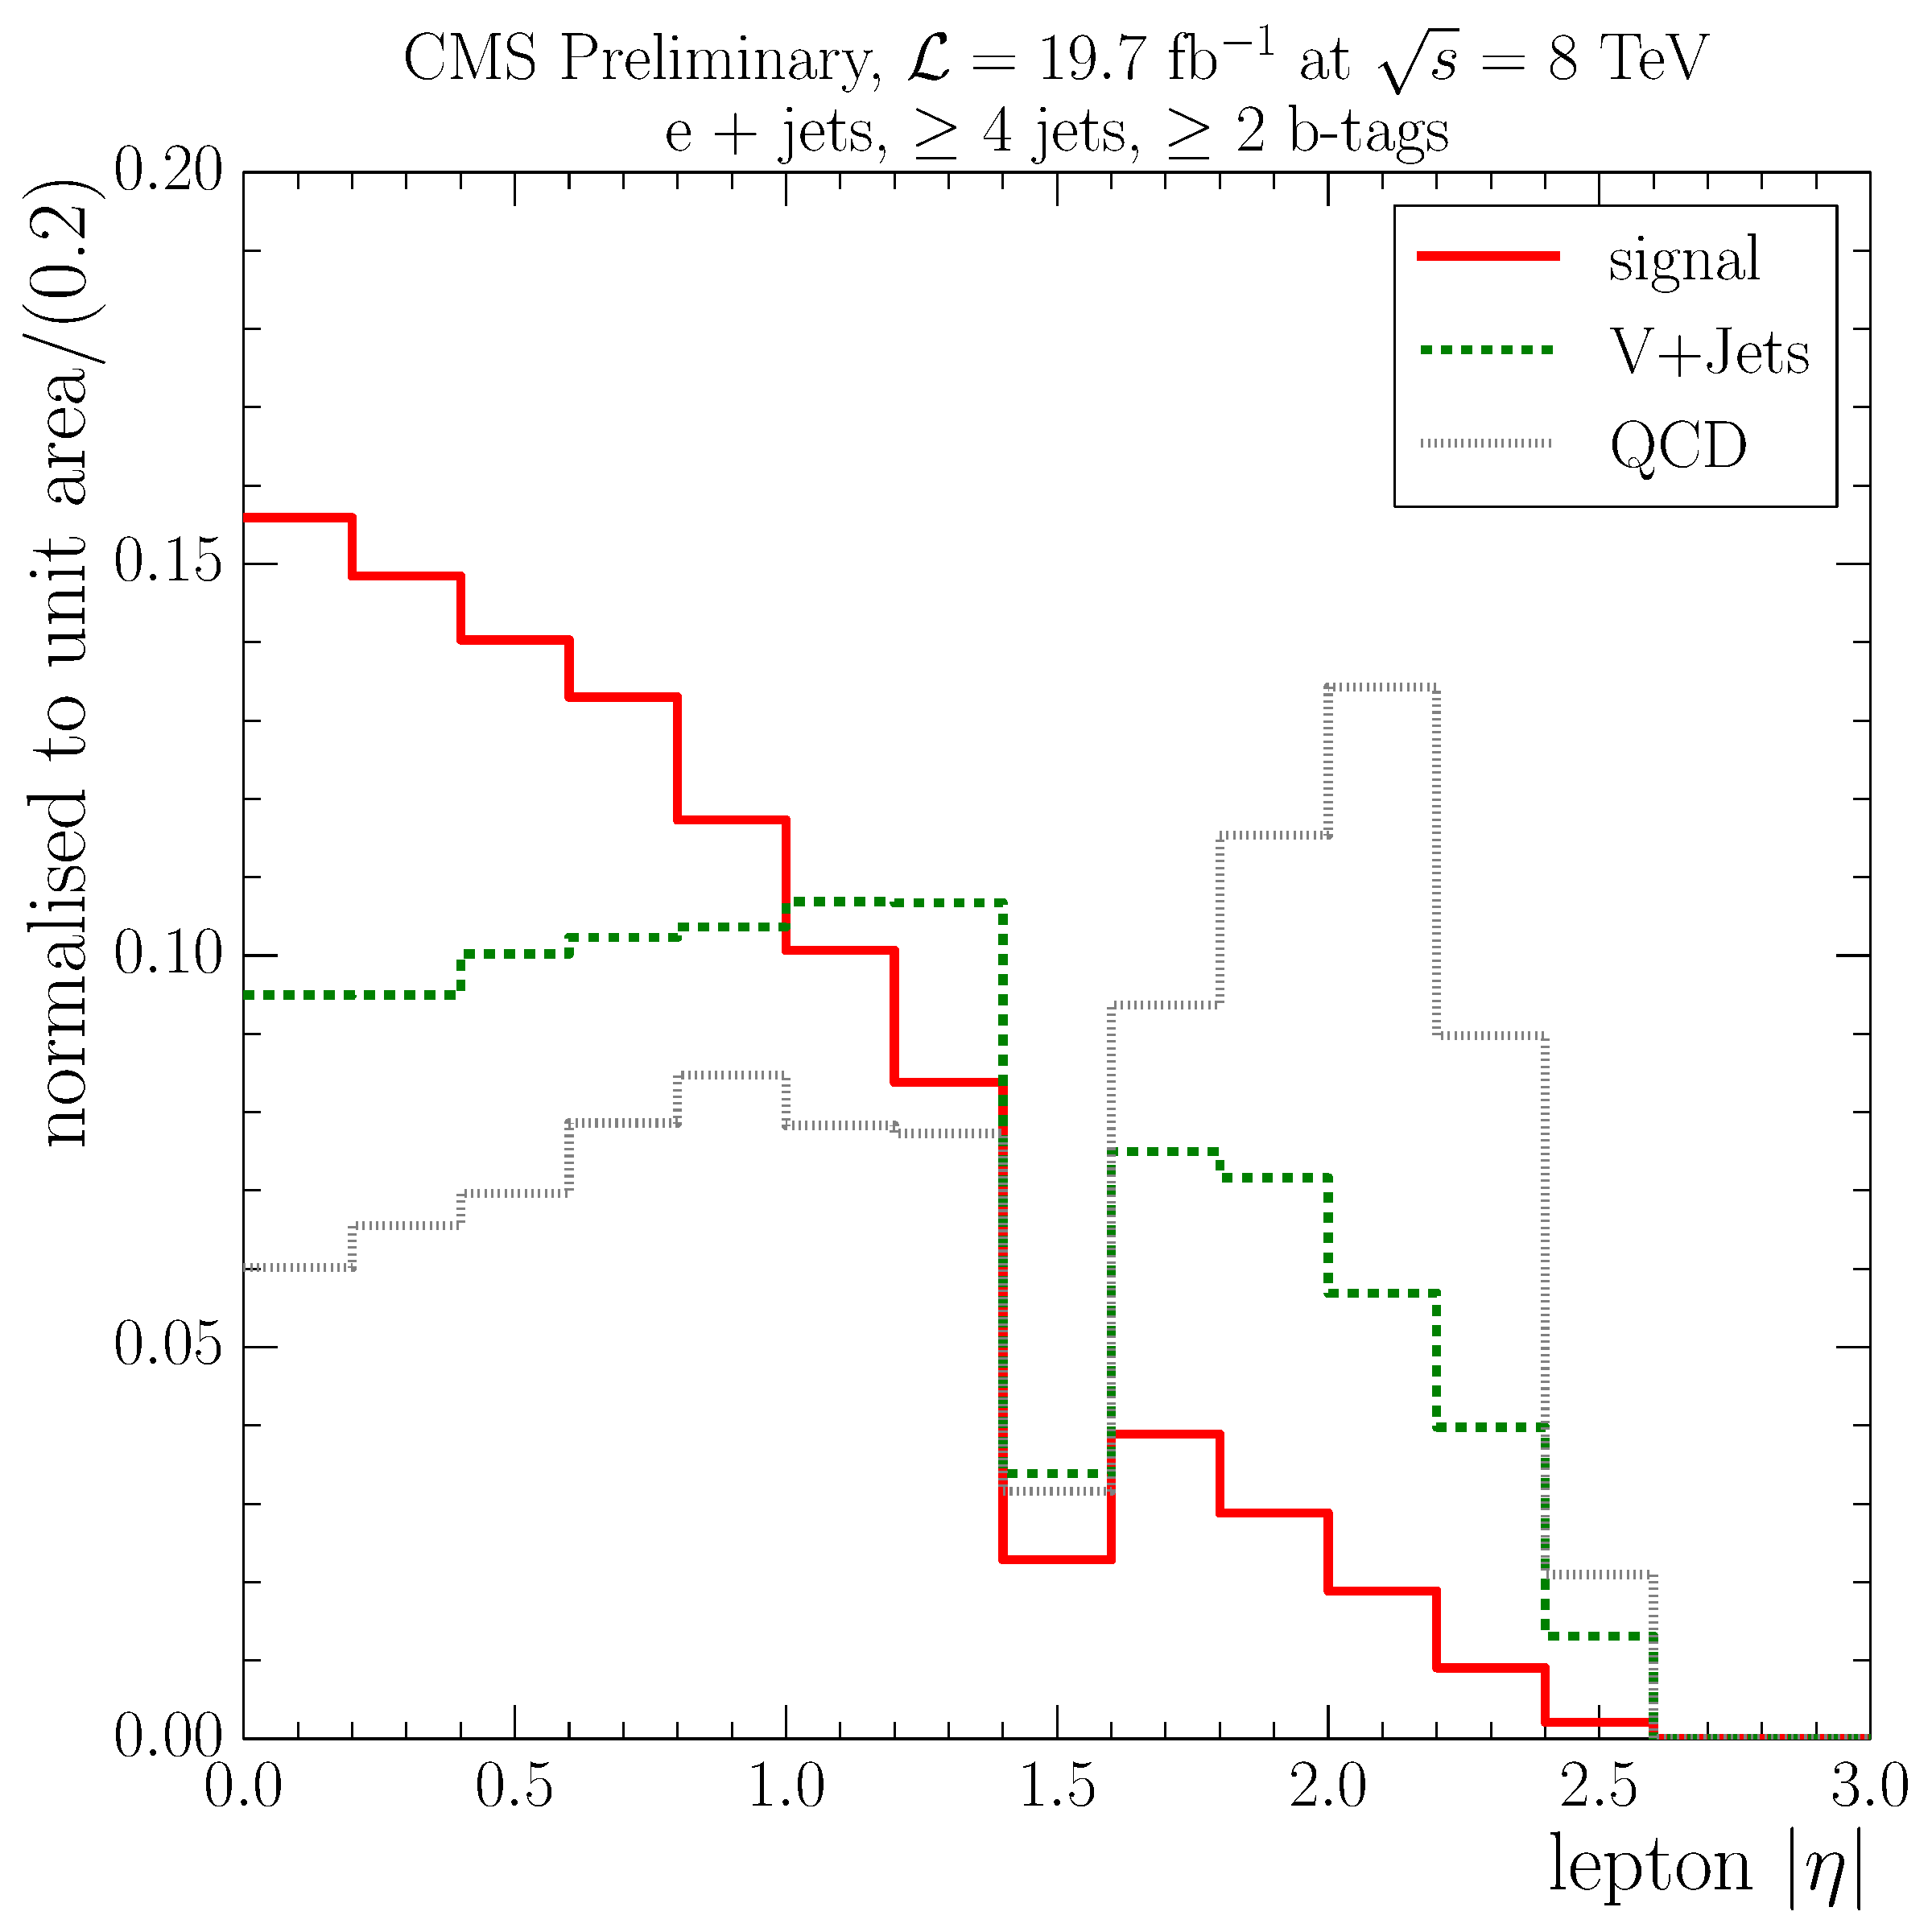
\includegraphics[width=0.39\textwidth]{measurement/WPT/central/fit_templates/electron_templates_bin_70-100}}\hfill
    {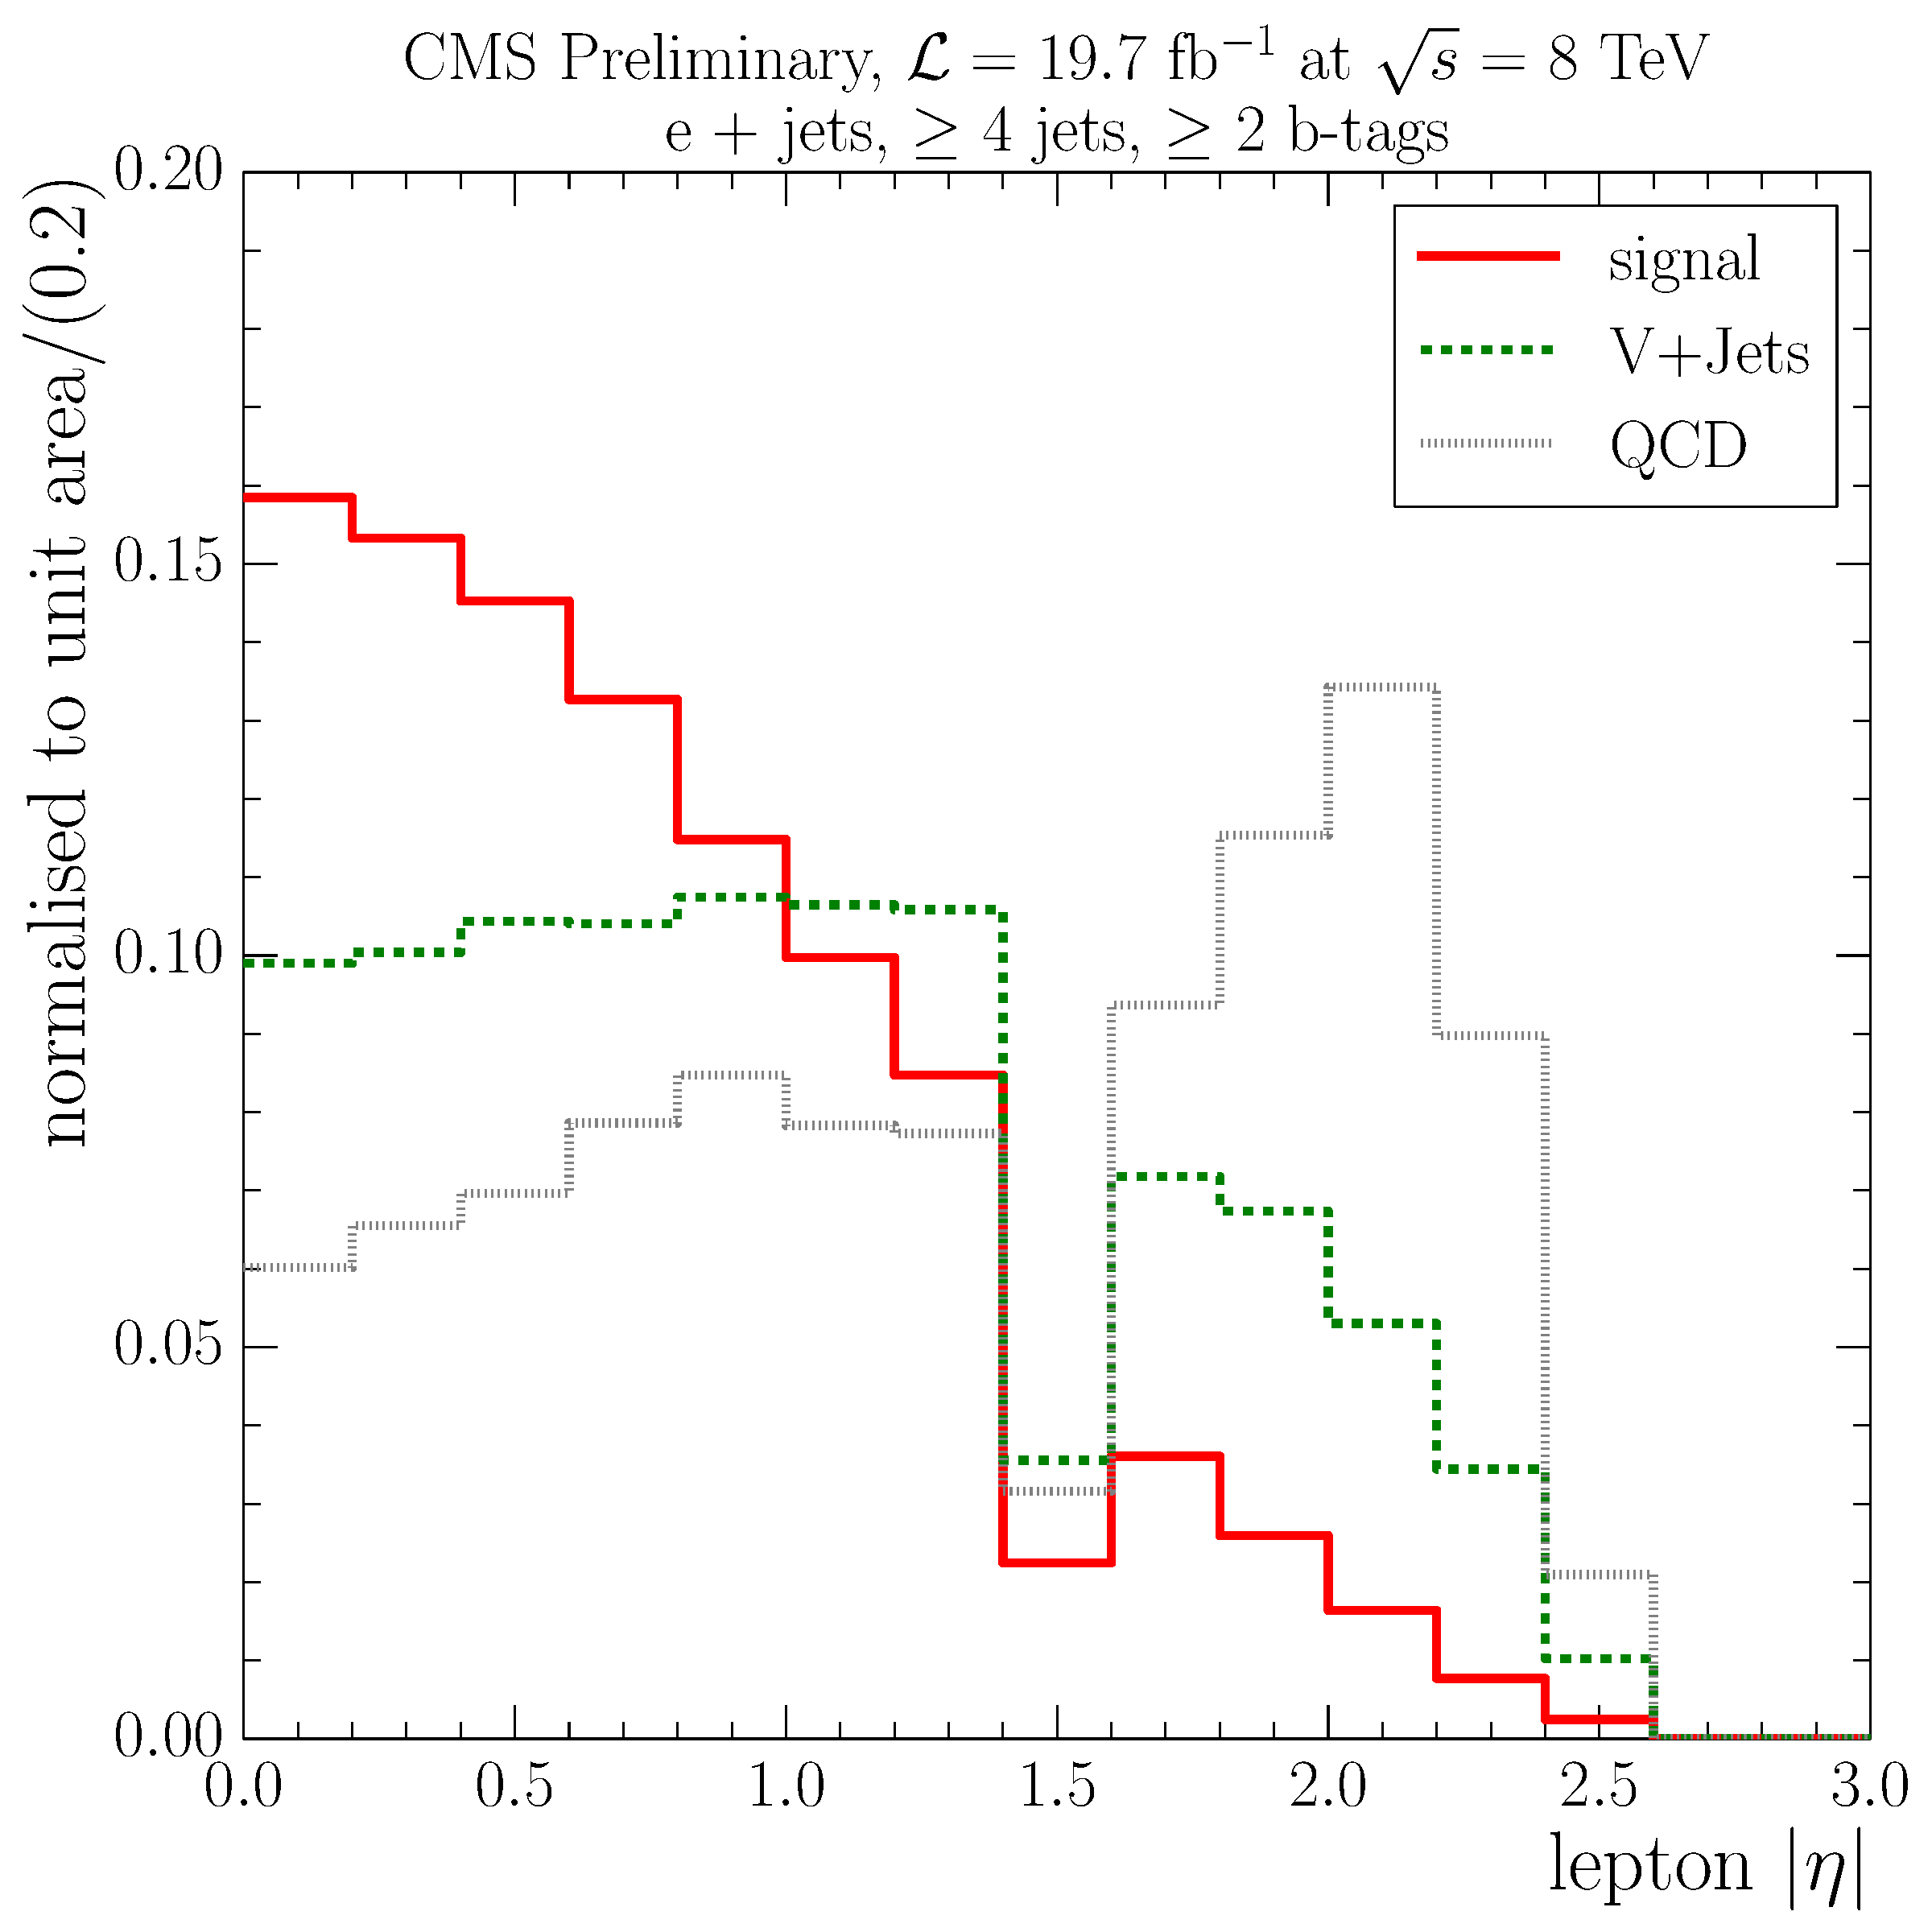
\includegraphics[width=0.39\textwidth]{measurement/WPT/central/fit_templates/electron_templates_bin_100-130}}
    \hspace*{\fill} \\
    \hspace*{\fill}
    {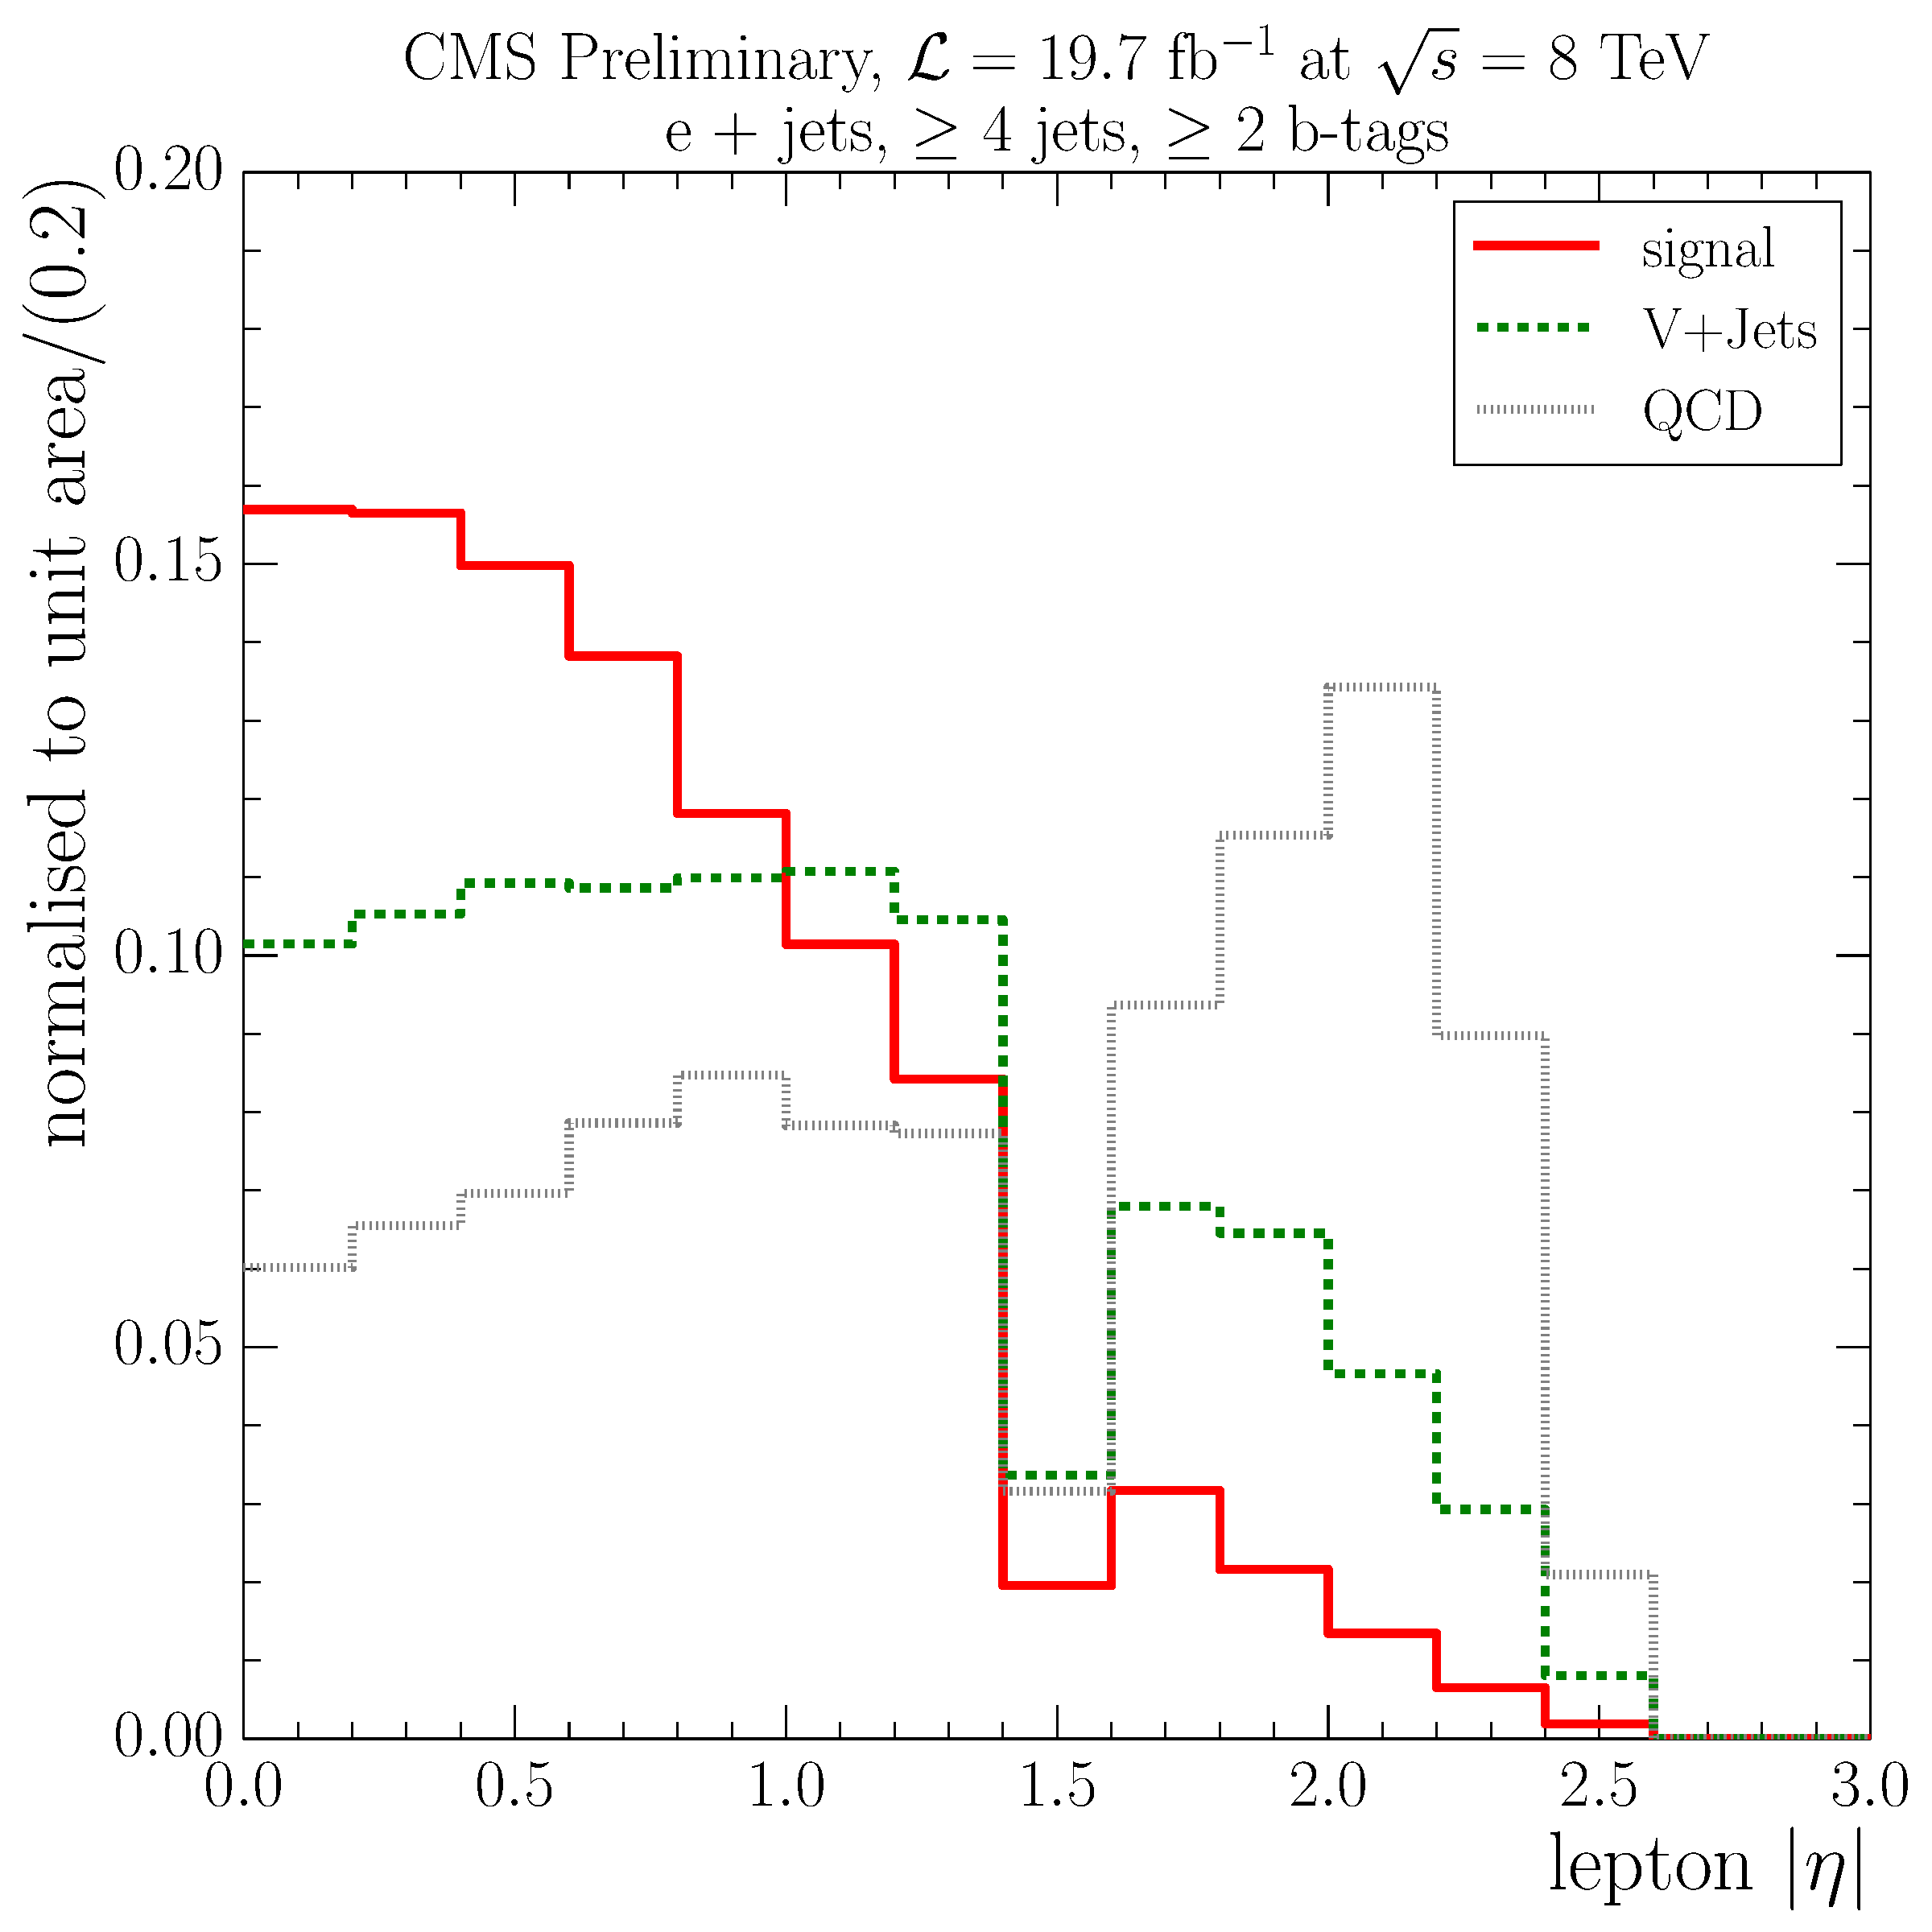
\includegraphics[width=0.39\textwidth]{measurement/WPT/central/fit_templates/electron_templates_bin_130-170}}\hfill
    {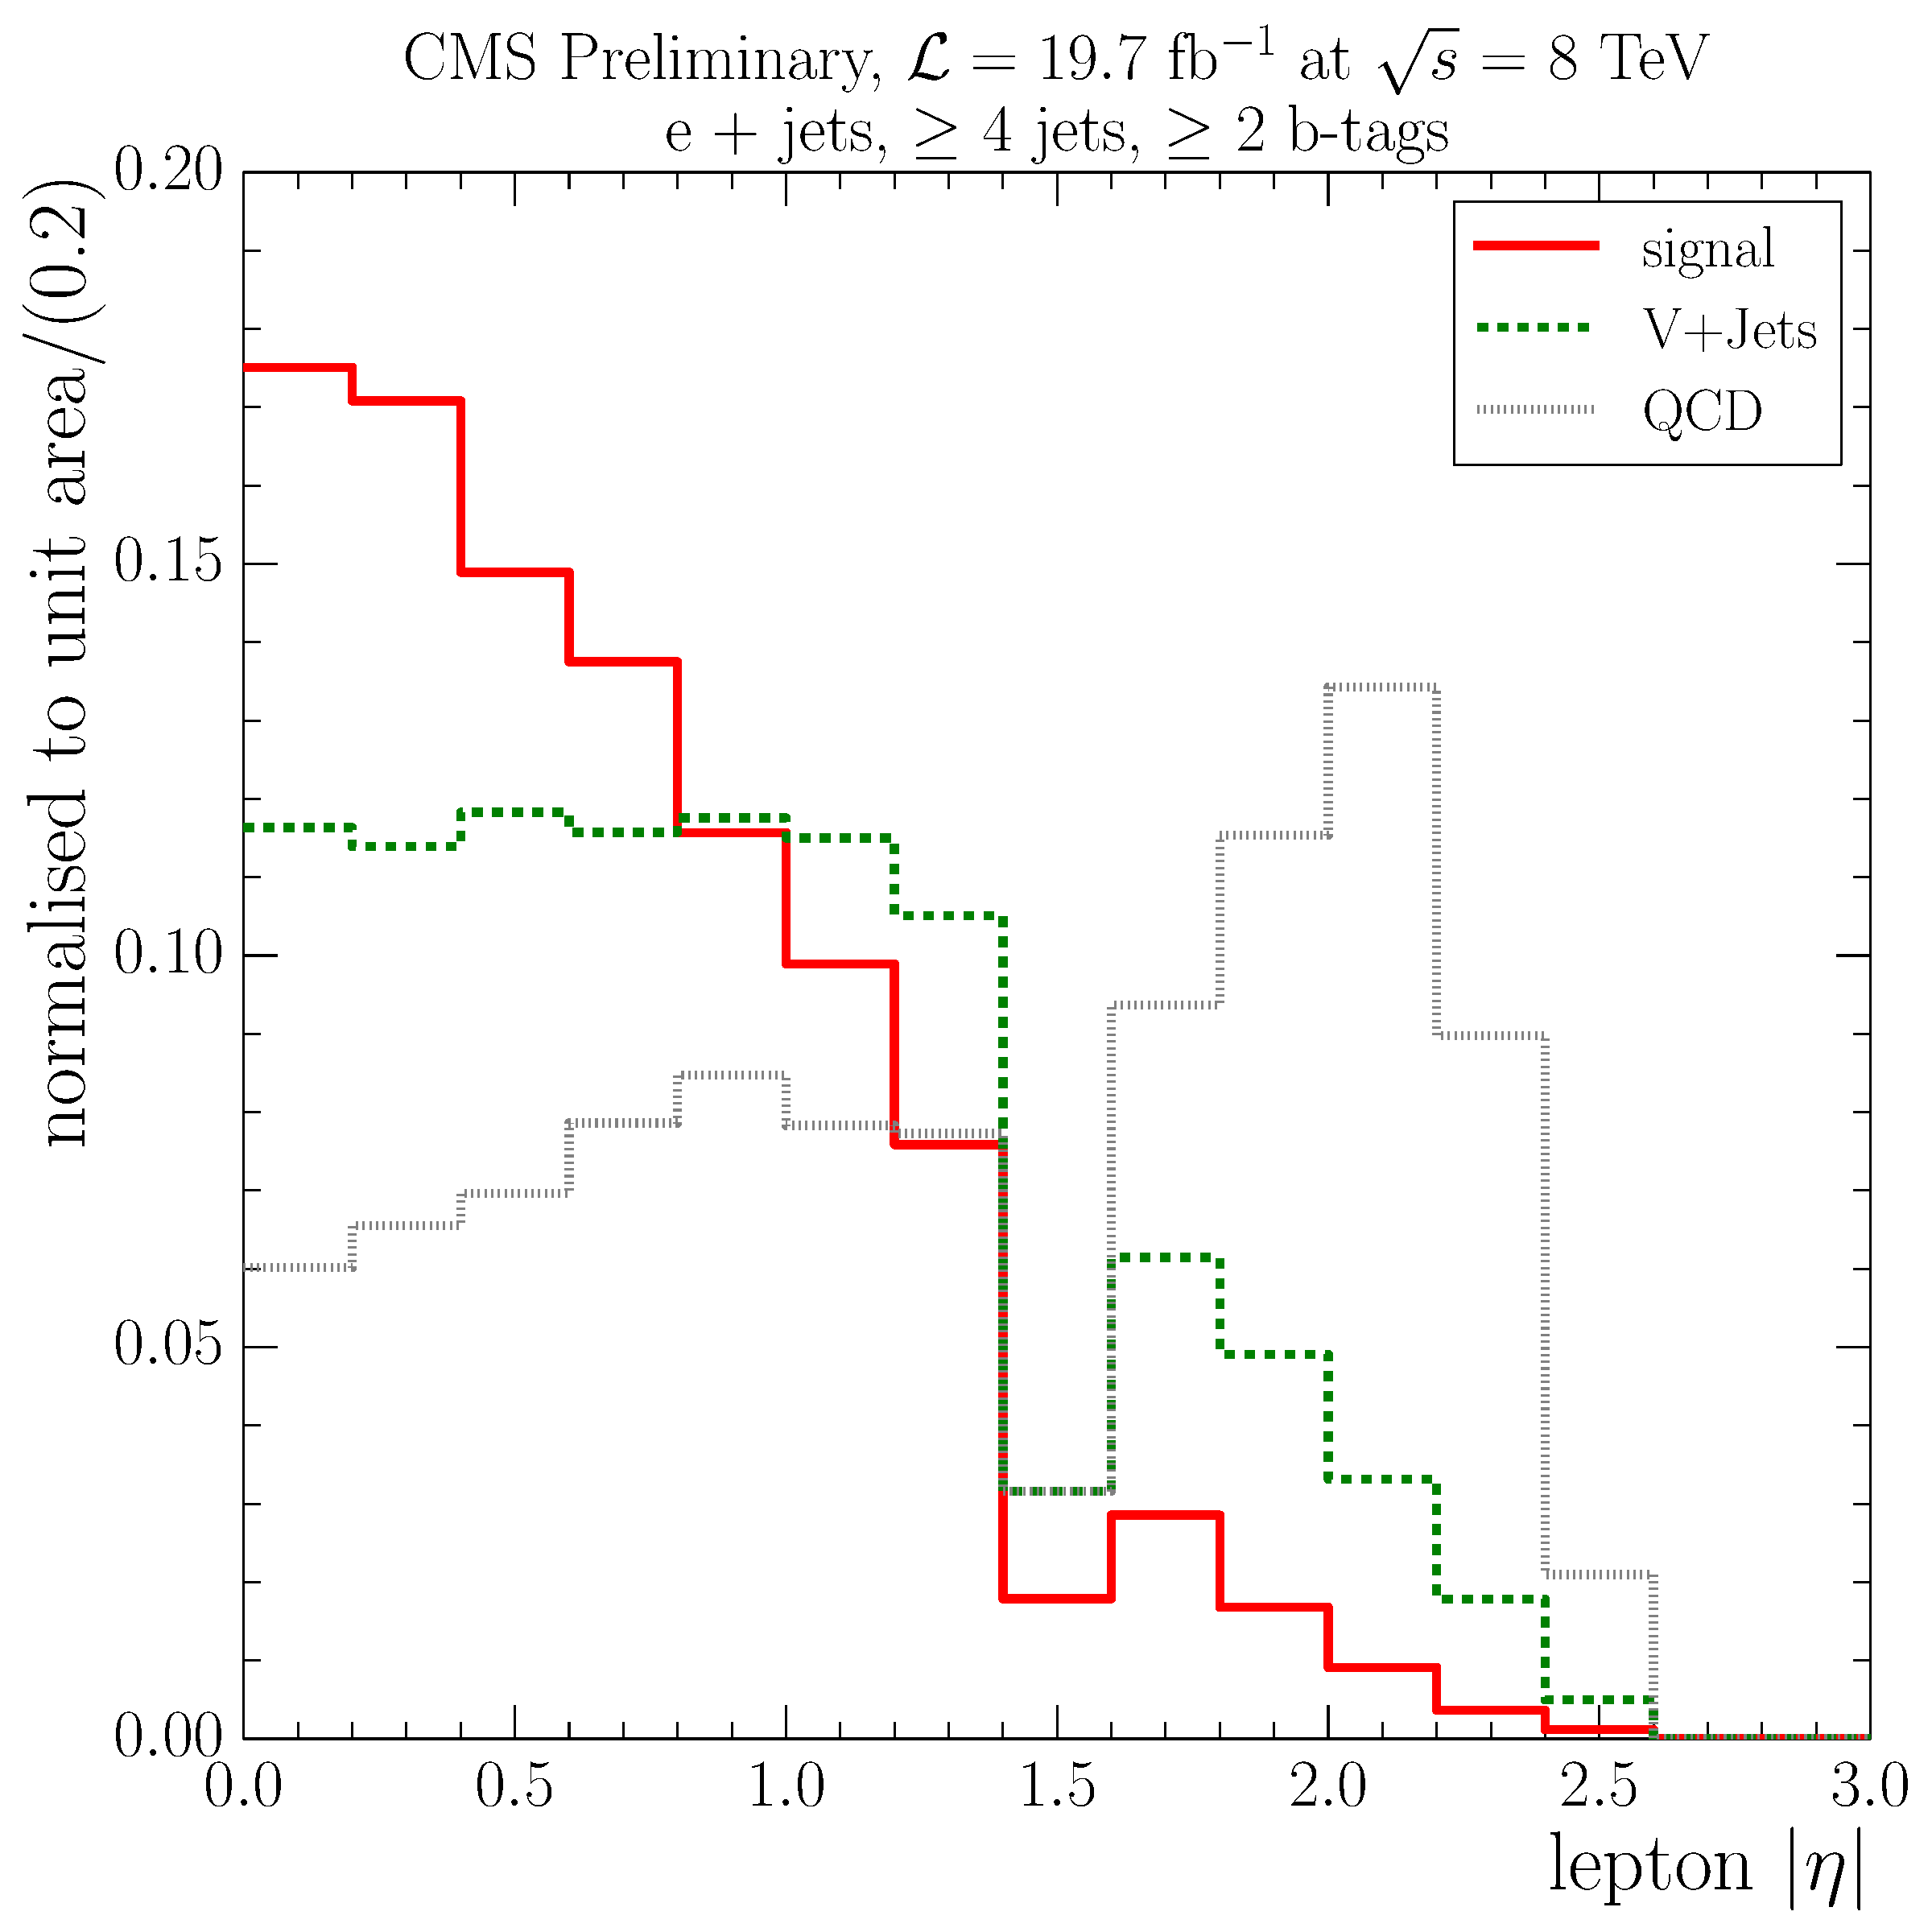
\includegraphics[width=0.39\textwidth]{measurement/WPT/central/fit_templates/electron_templates_bin_170-inf}}
    \hspace*{\fill}
    \caption[Electron $\abs \eta$ templates for the fit in different bins of \WPT]{Electron $\abs \eta$ templates for
    the fit in different bins of \WPT, from top left to bottom right: \SIrange{0}{40}{\GeV}, \SIrange{40}{70}{\GeV},
    \SIrange{70}{100}{\GeV}, \SIrange{100}{130}{\GeV}, \SIrange{130}{170}{\GeV} and $\geq \SI{170}{\GeV}$.}
    \label{fig:fit_tempaltes_WPT_electron}
\end{figure}

\begin{figure}[!htbp]
  \centering
    \hspace*{\fill}
    {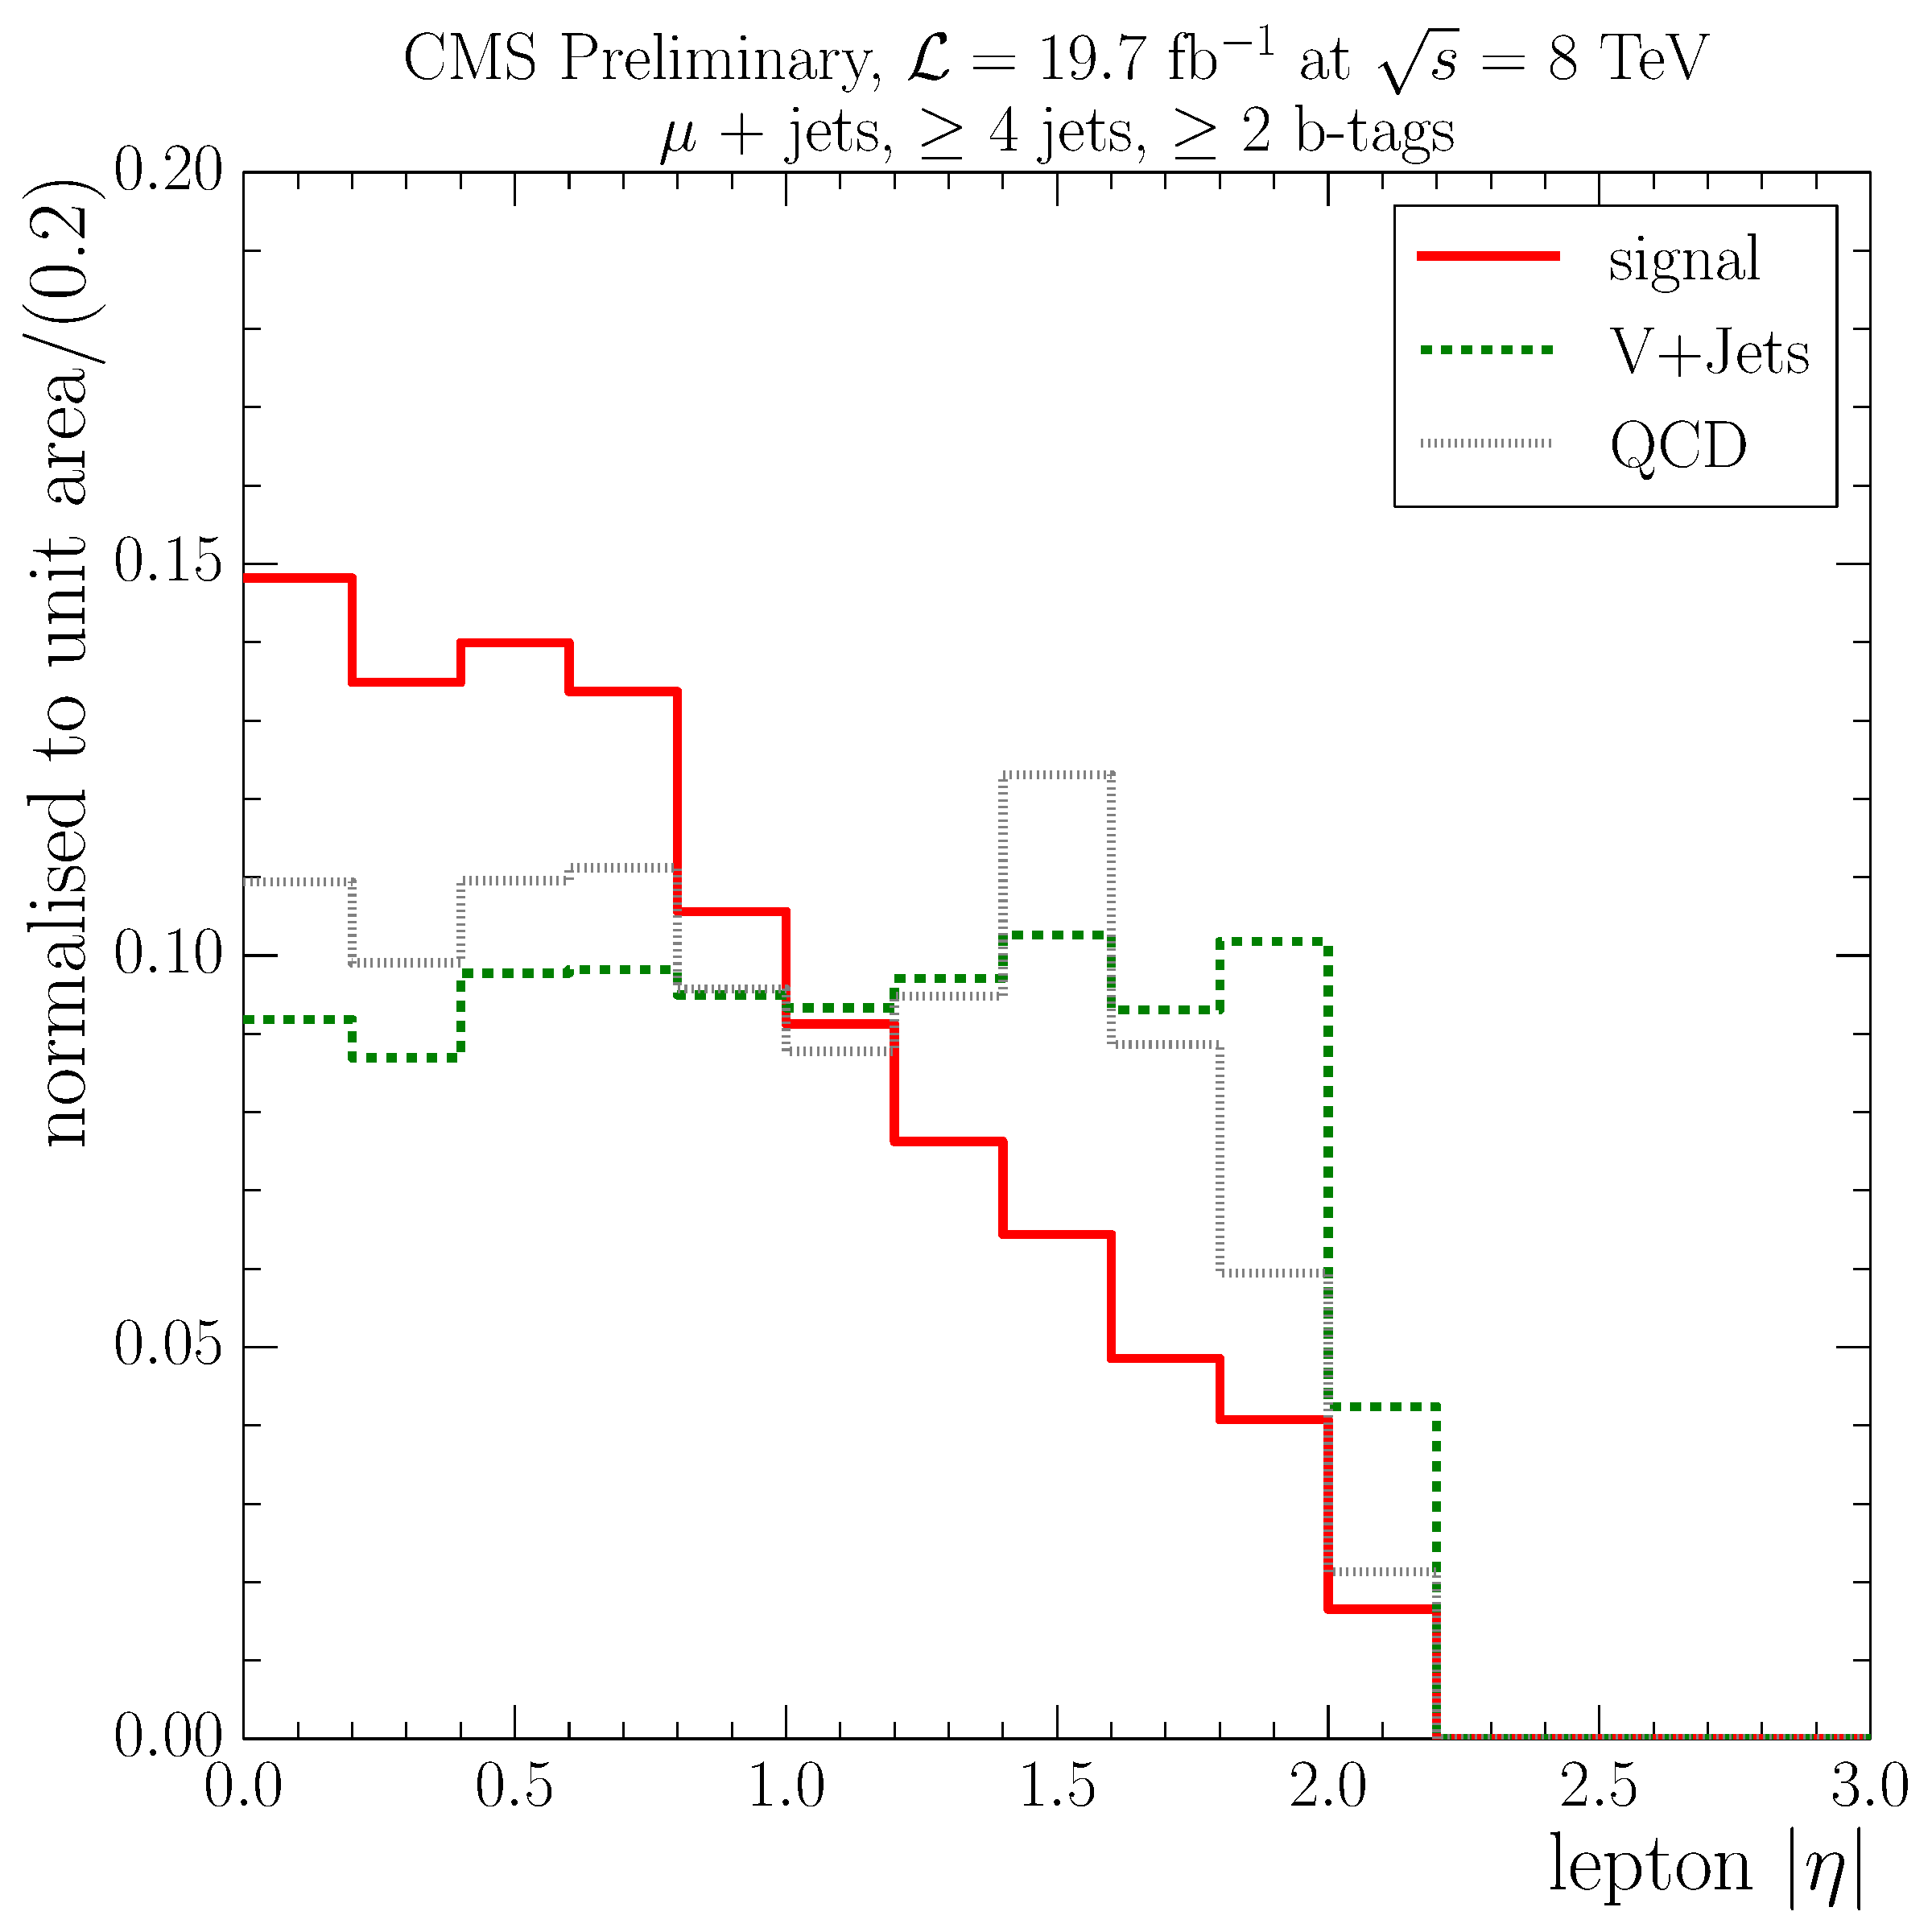
\includegraphics[width=0.39\textwidth]{measurement/WPT/central/fit_templates/muon_templates_bin_0-40}}\hfill
    {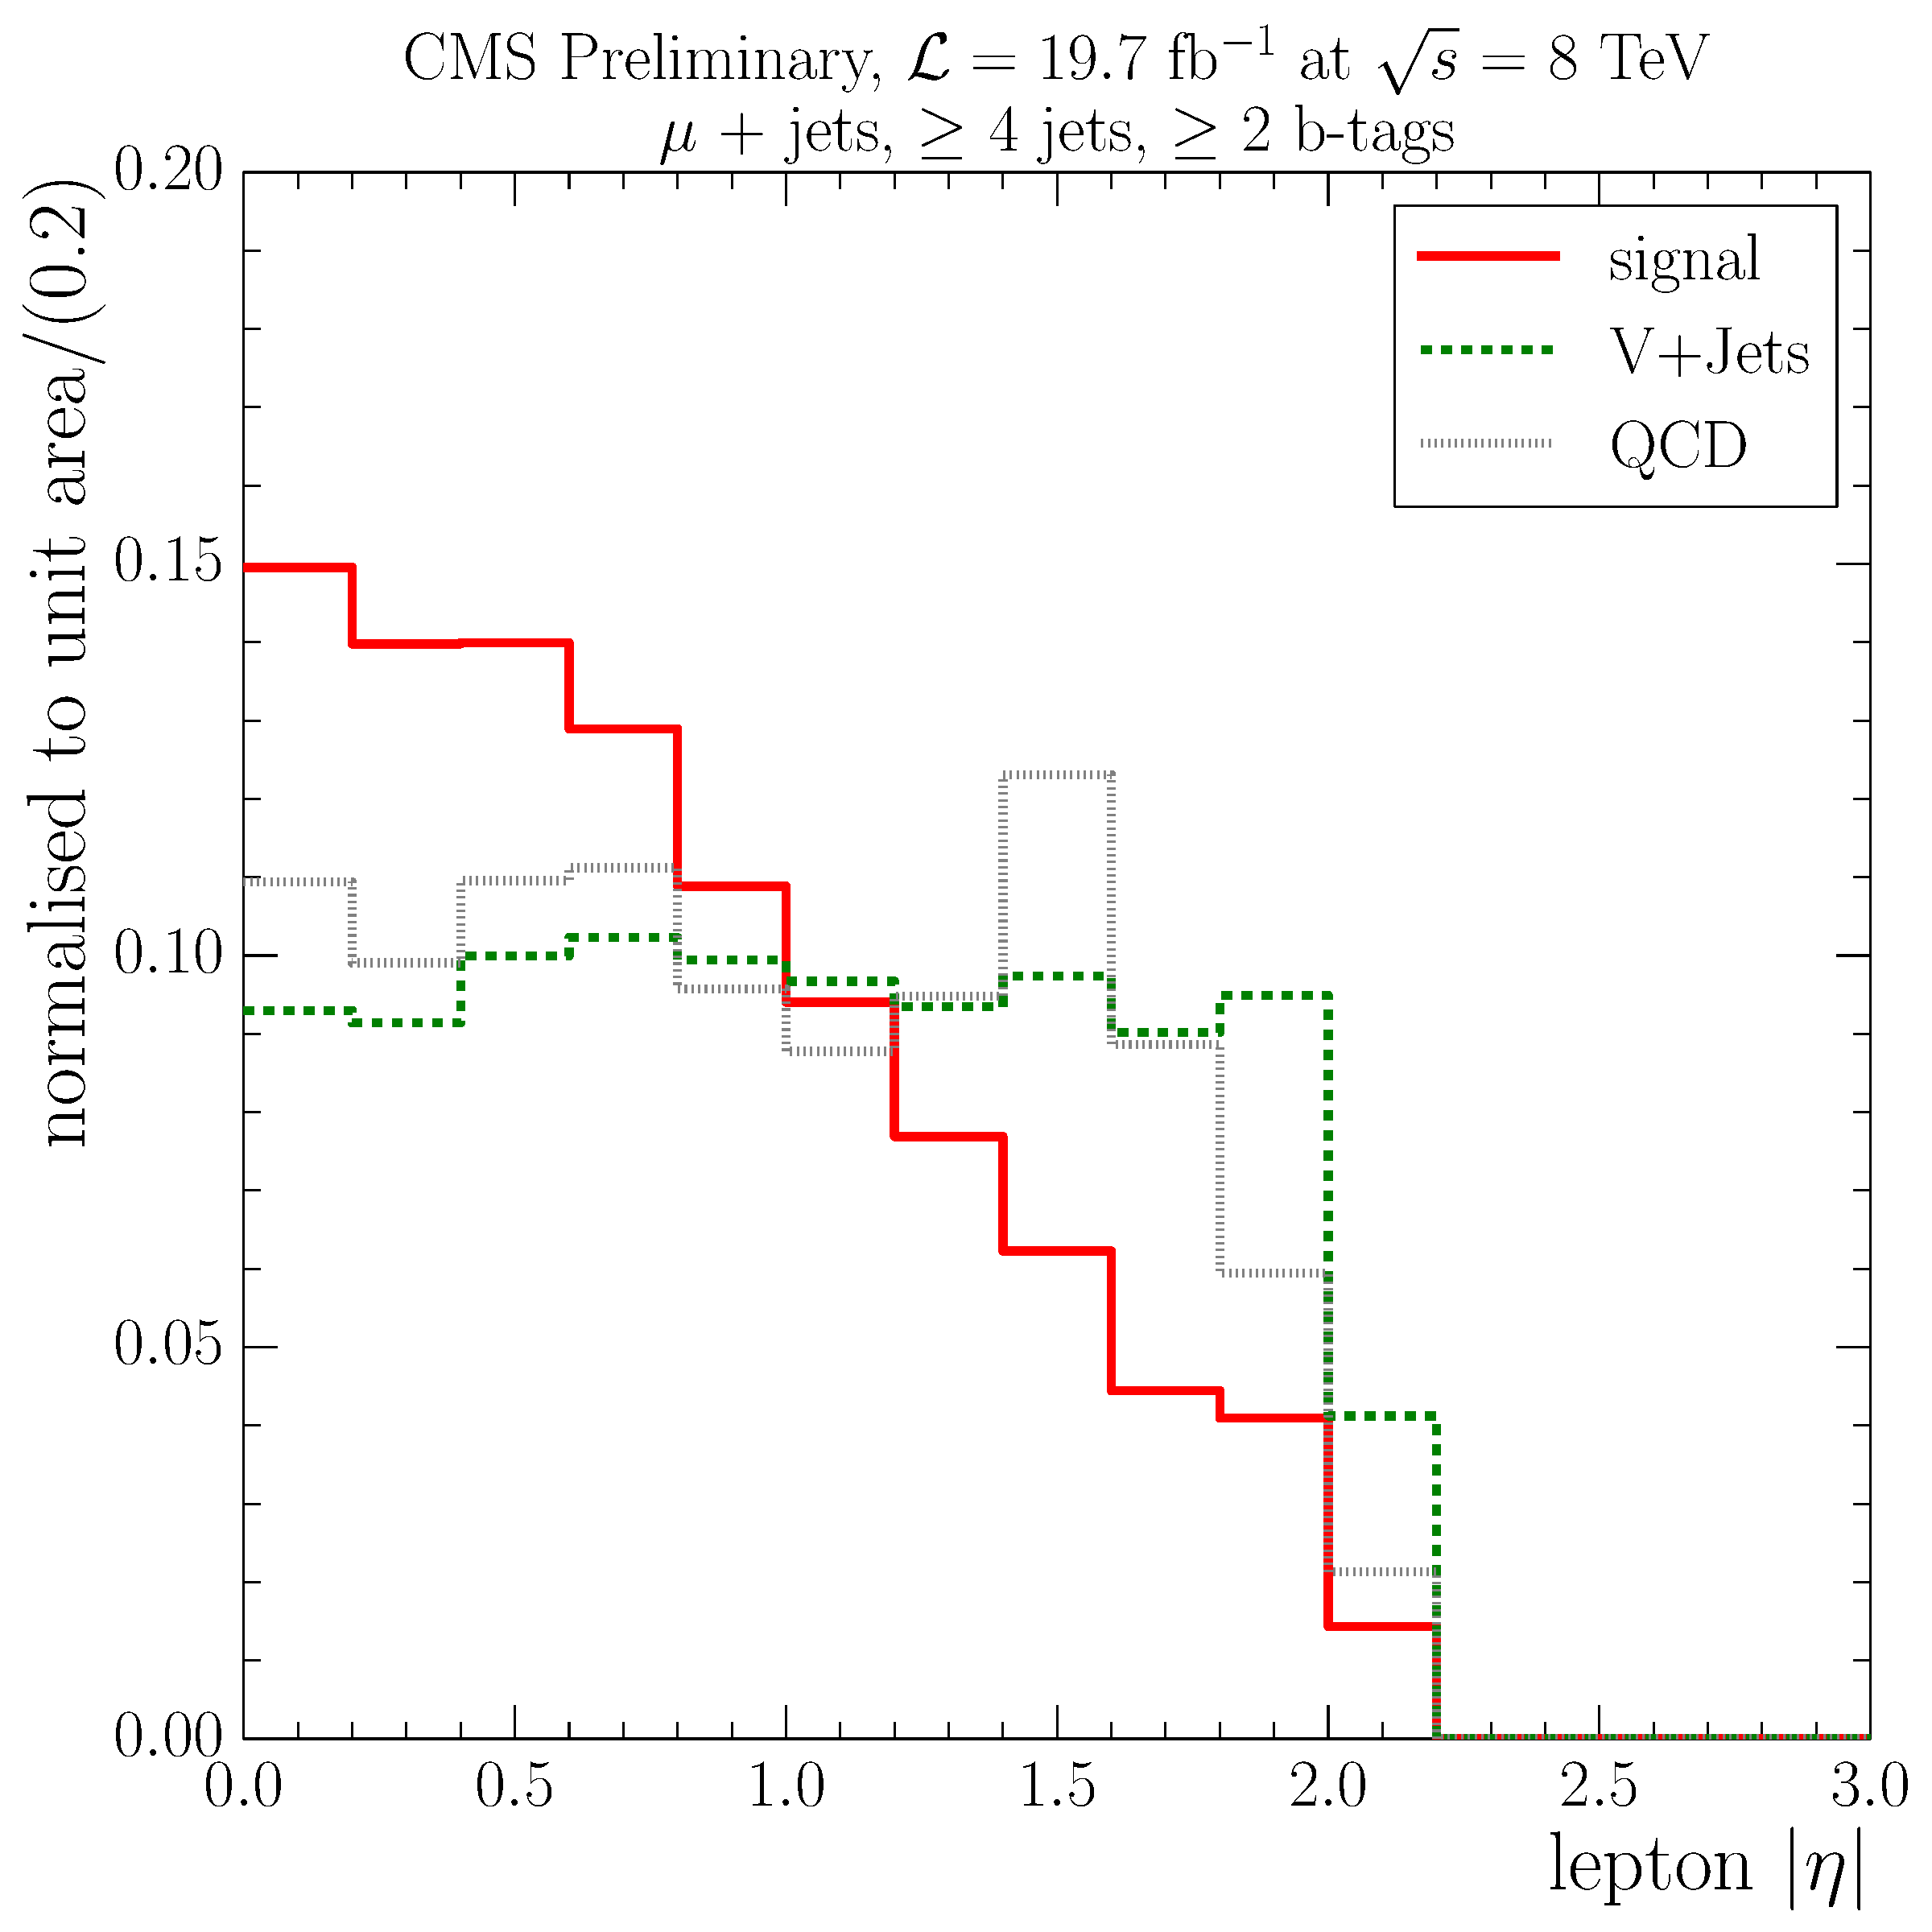
\includegraphics[width=0.39\textwidth]{measurement/WPT/central/fit_templates/muon_templates_bin_40-70}}
    \hspace*{\fill} \\
    \hspace*{\fill}
    {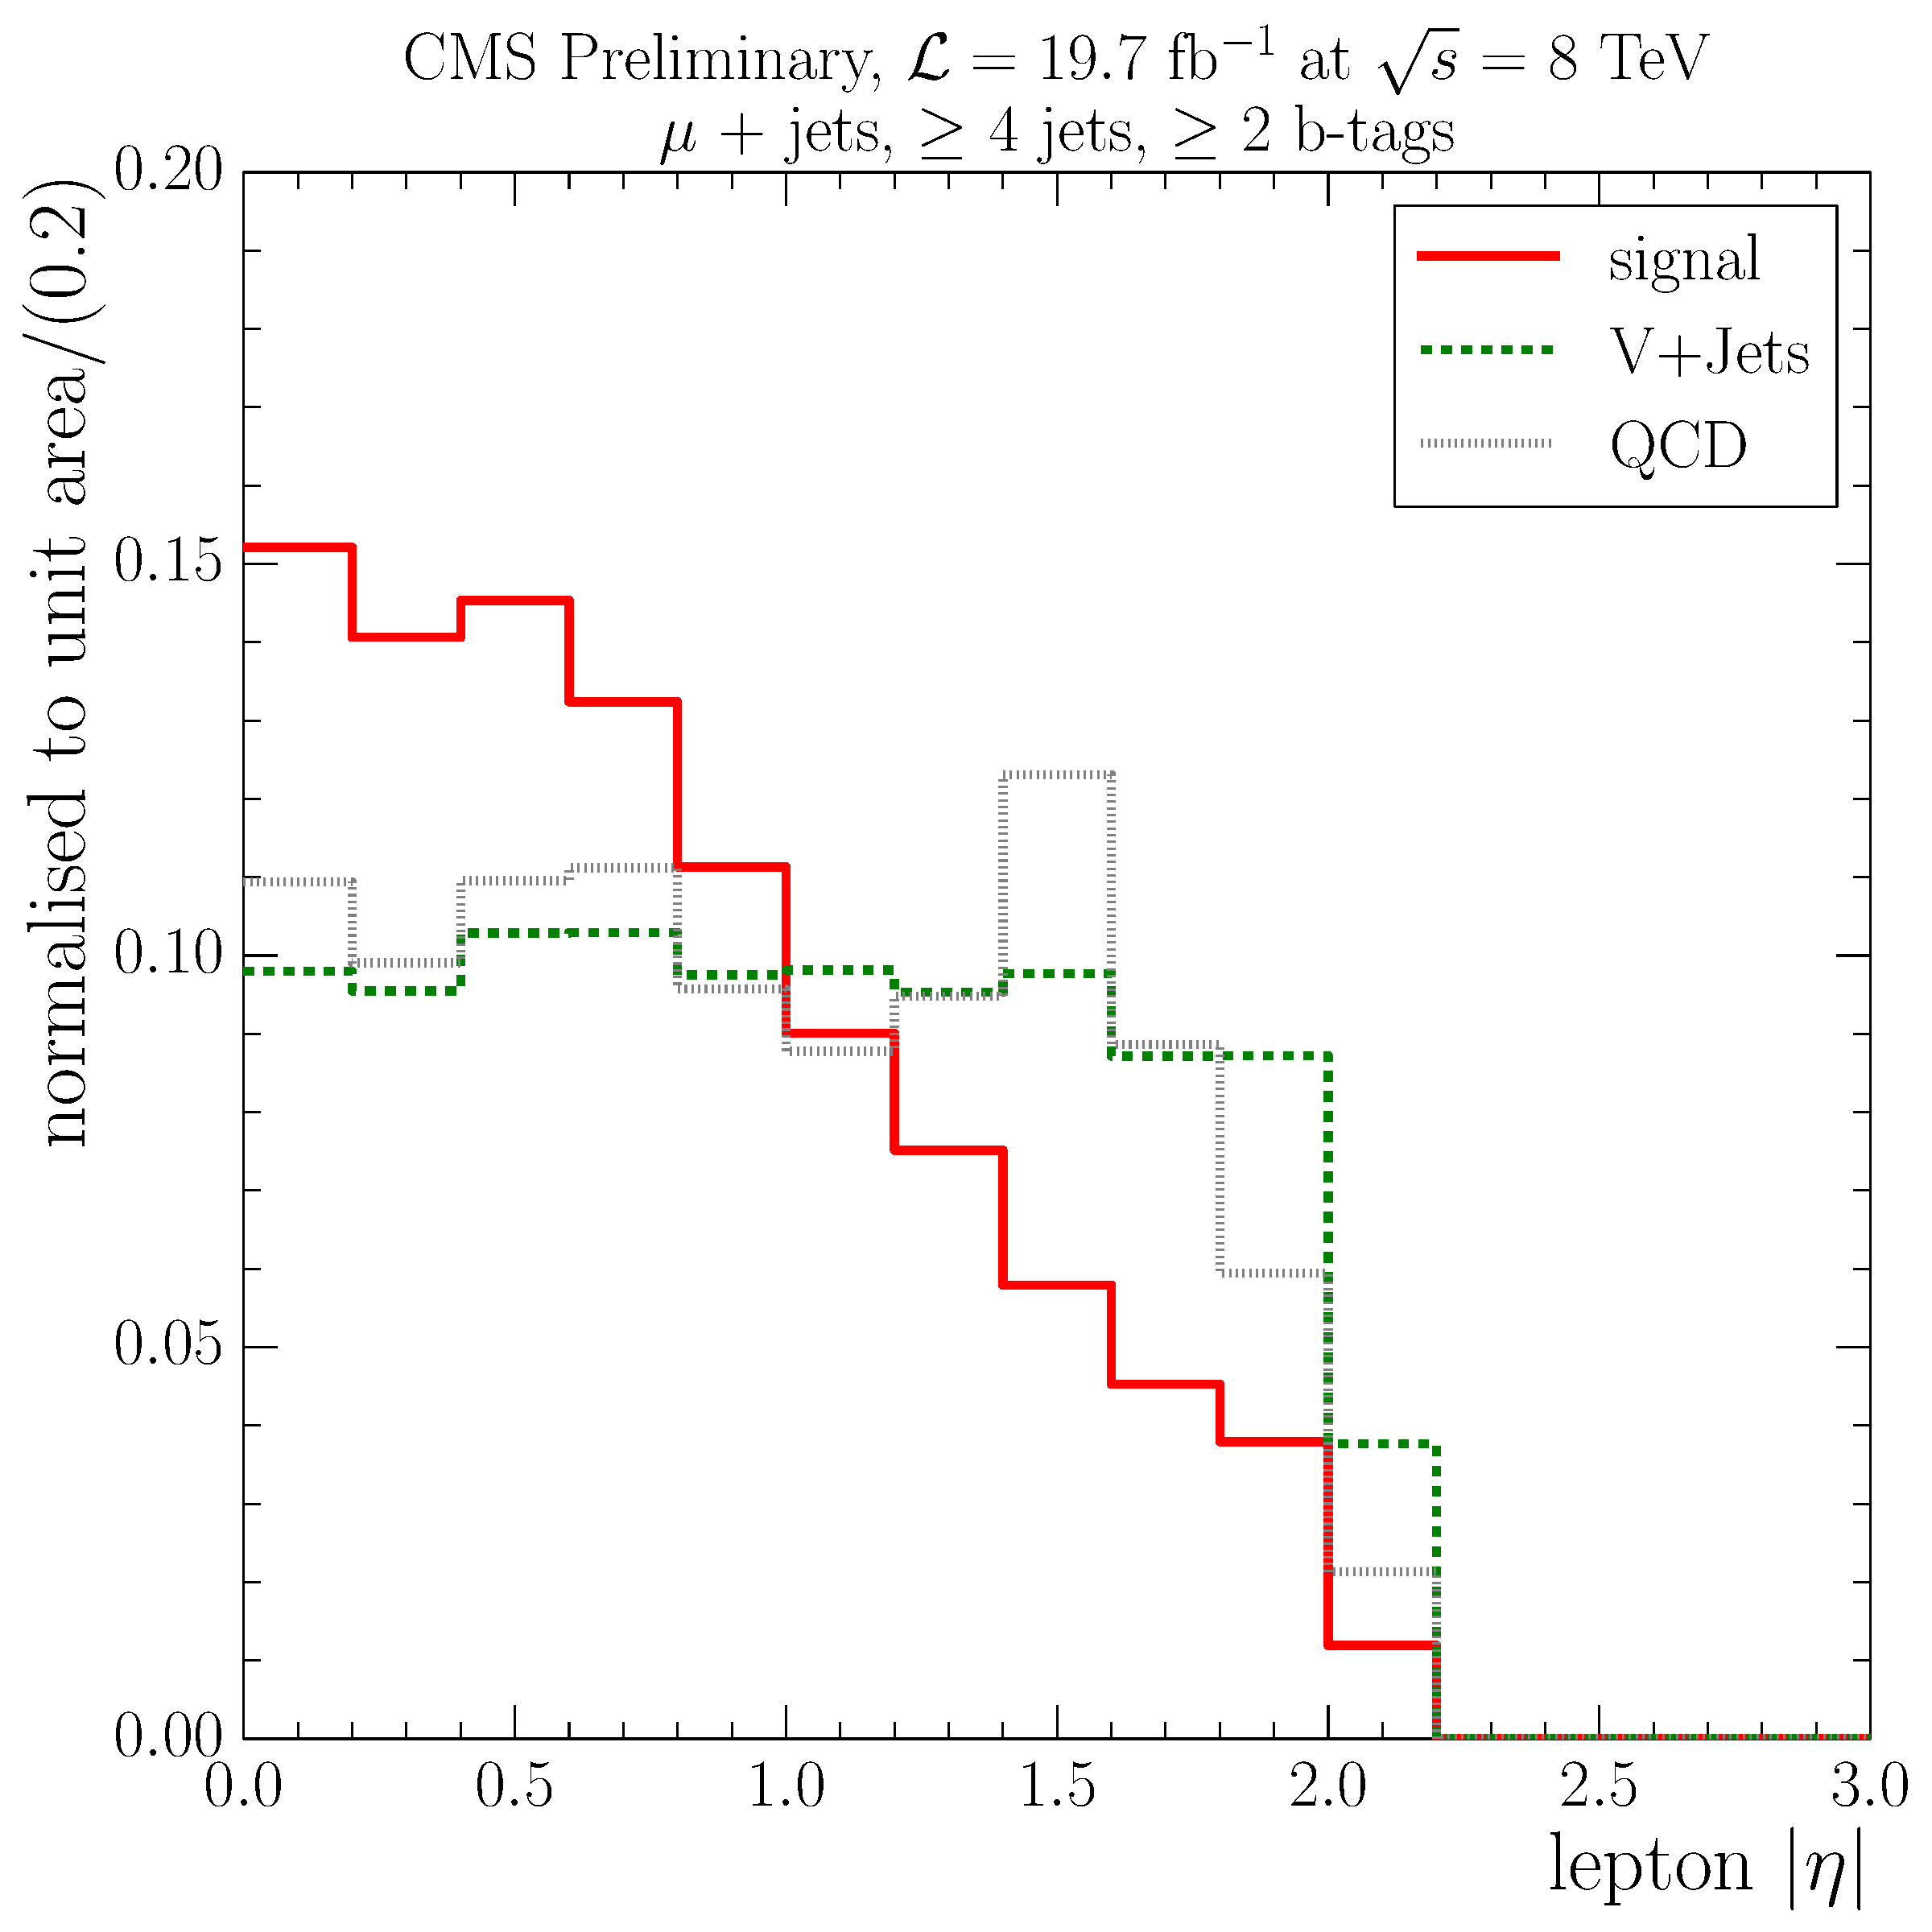
\includegraphics[width=0.39\textwidth]{measurement/WPT/central/fit_templates/muon_templates_bin_70-100}}\hfill
    {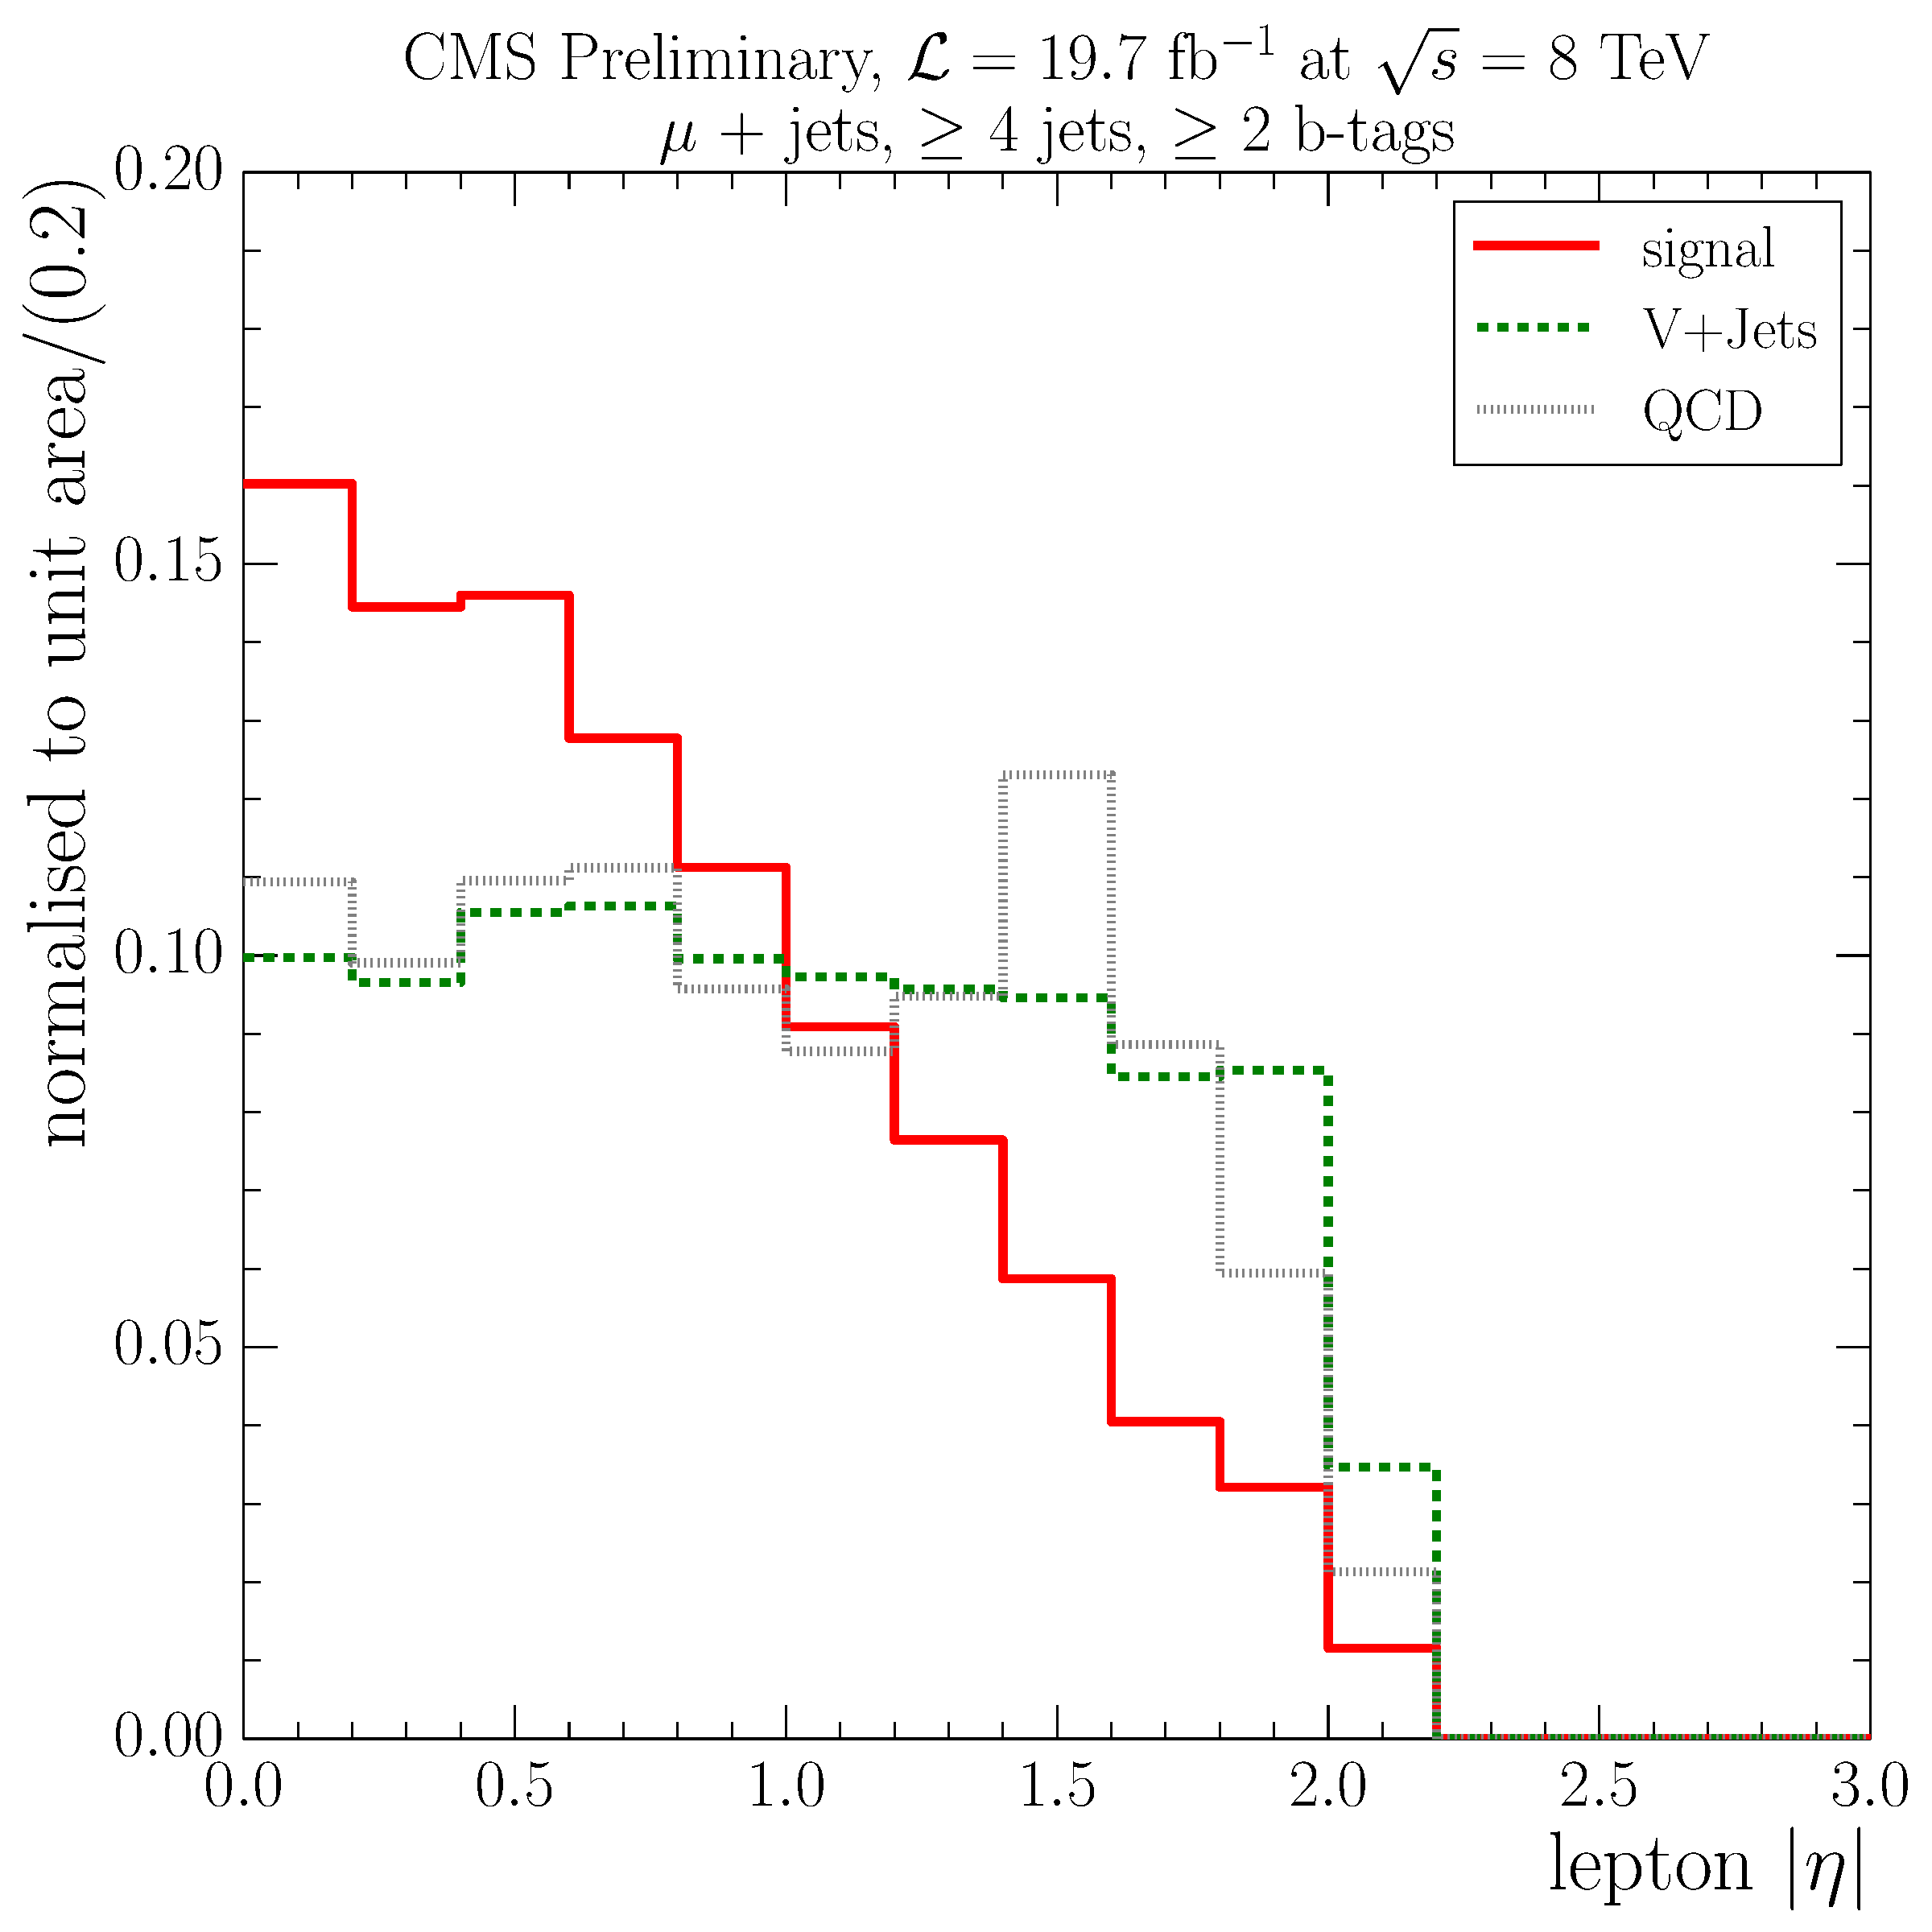
\includegraphics[width=0.39\textwidth]{measurement/WPT/central/fit_templates/muon_templates_bin_100-130}}
    \hspace*{\fill} \\
    \hspace*{\fill}
    {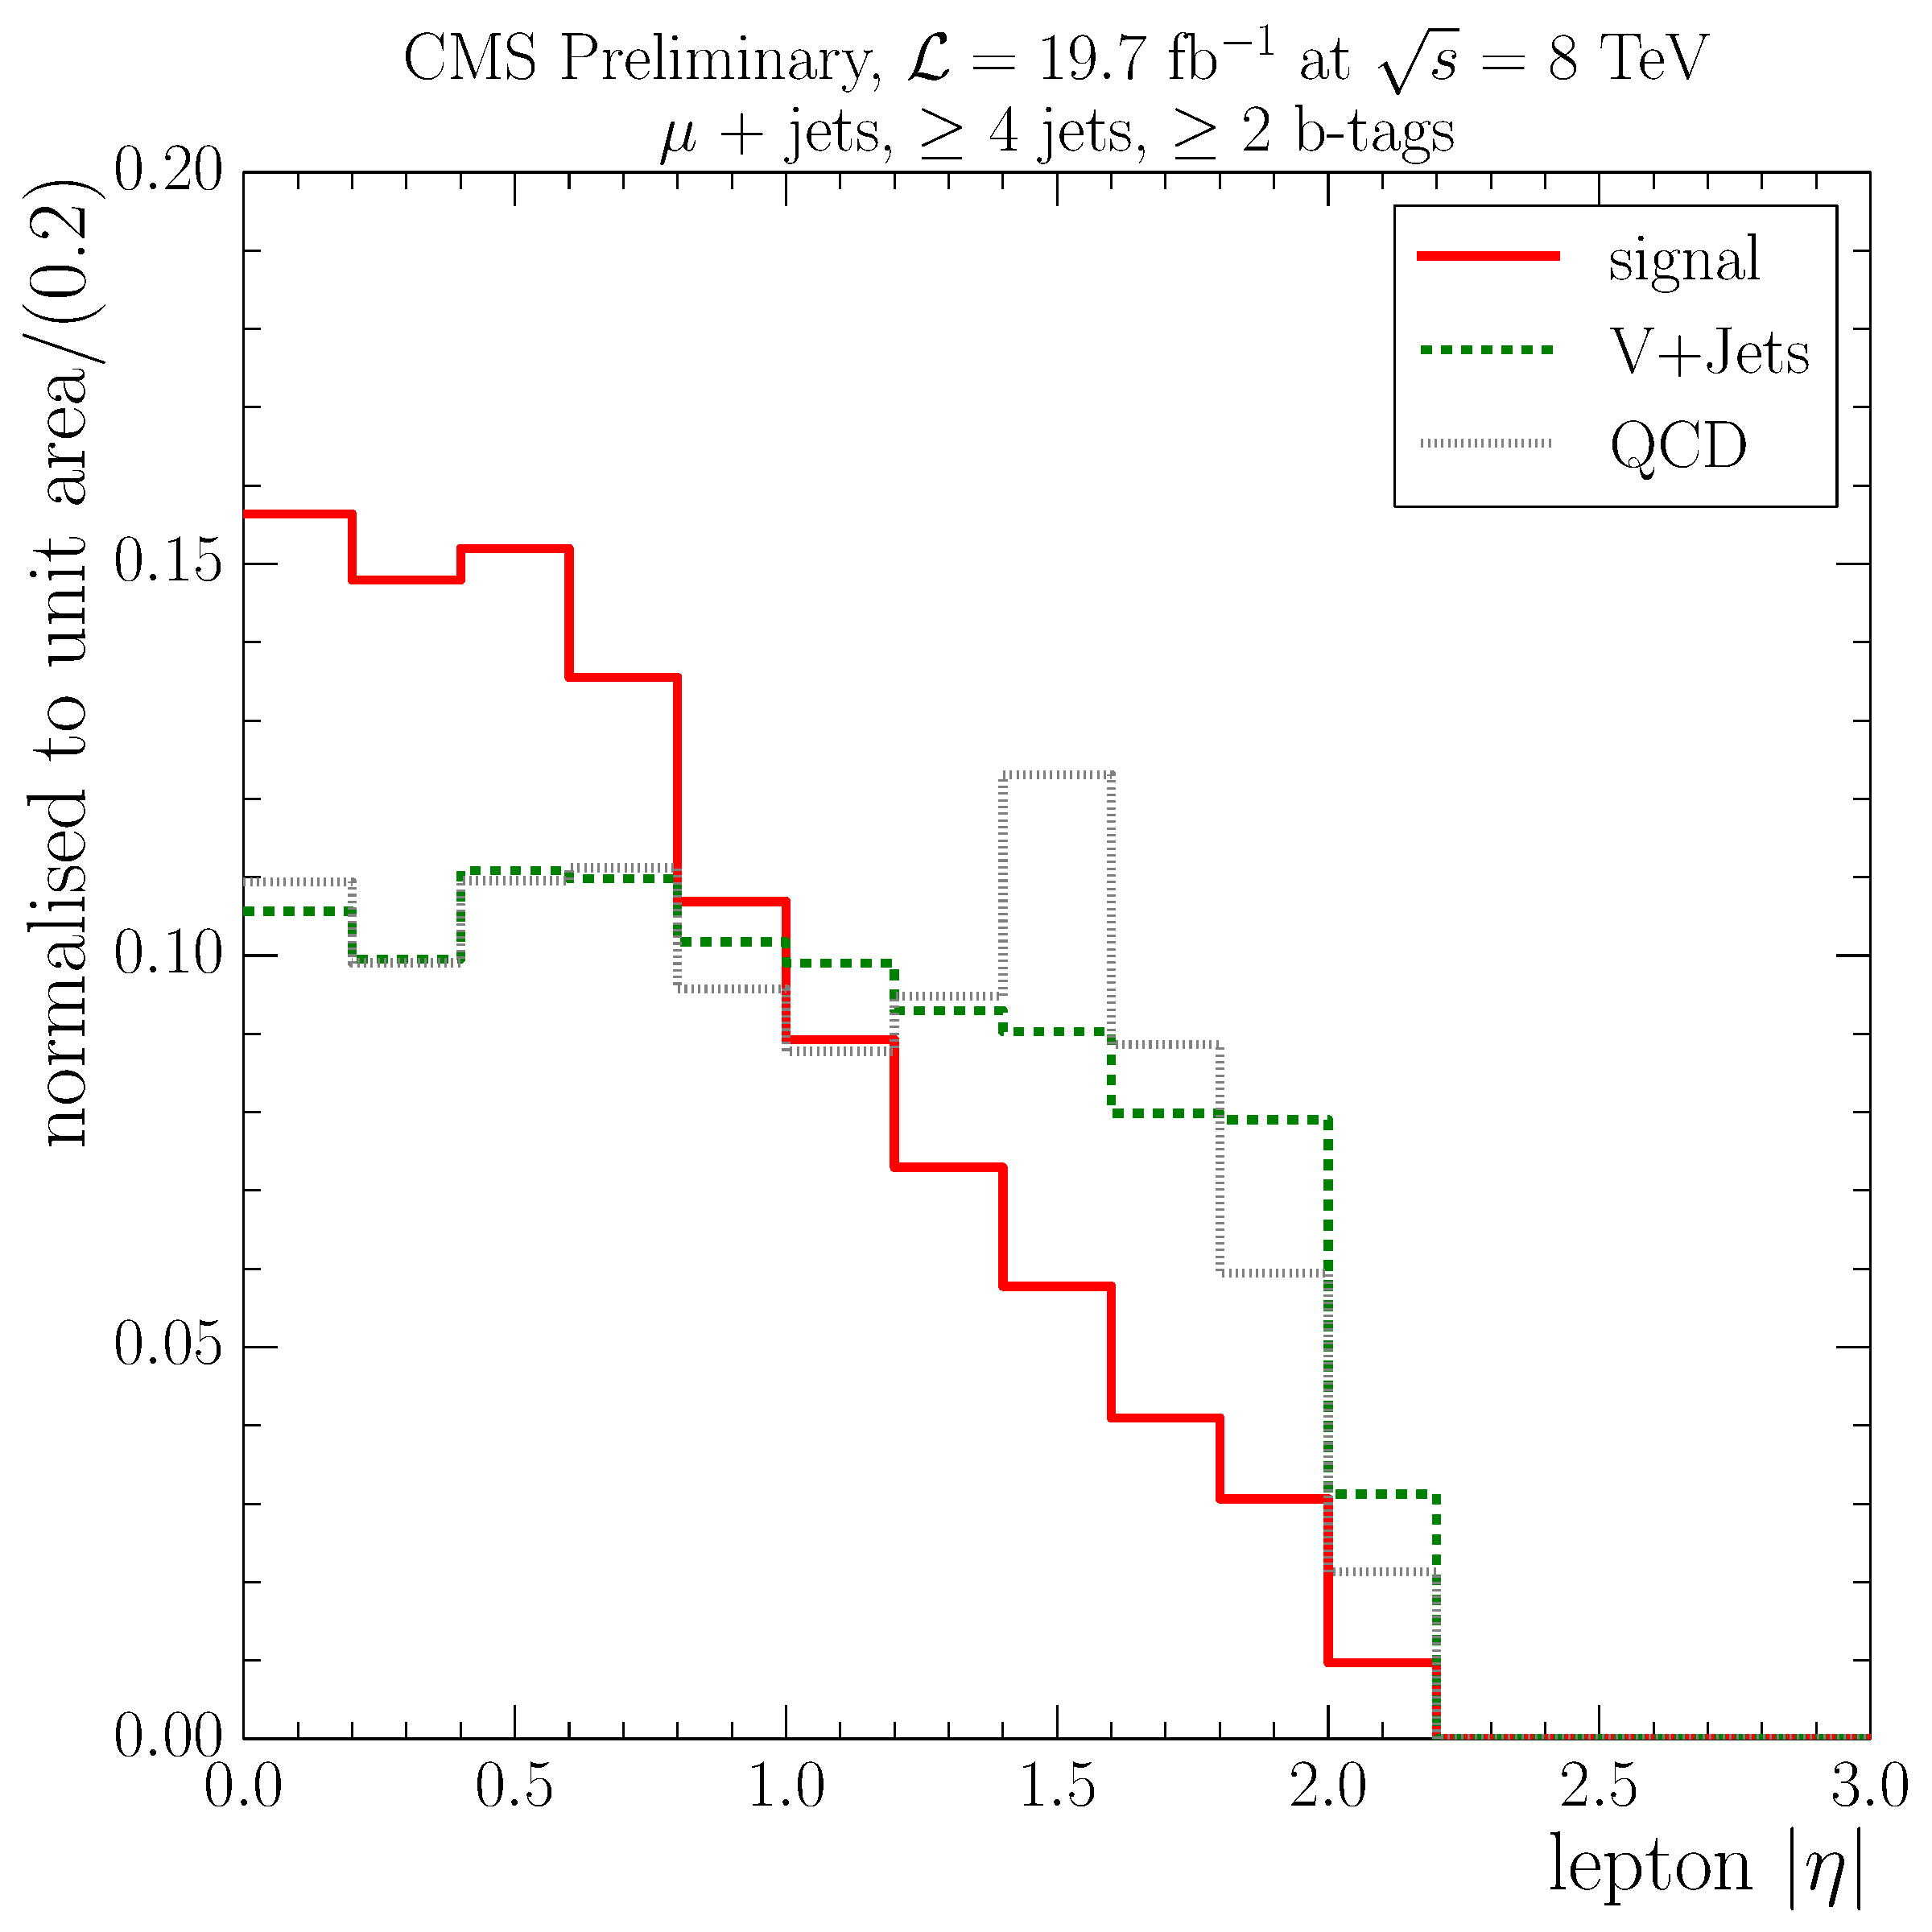
\includegraphics[width=0.39\textwidth]{measurement/WPT/central/fit_templates/muon_templates_bin_130-170}}\hfill
    {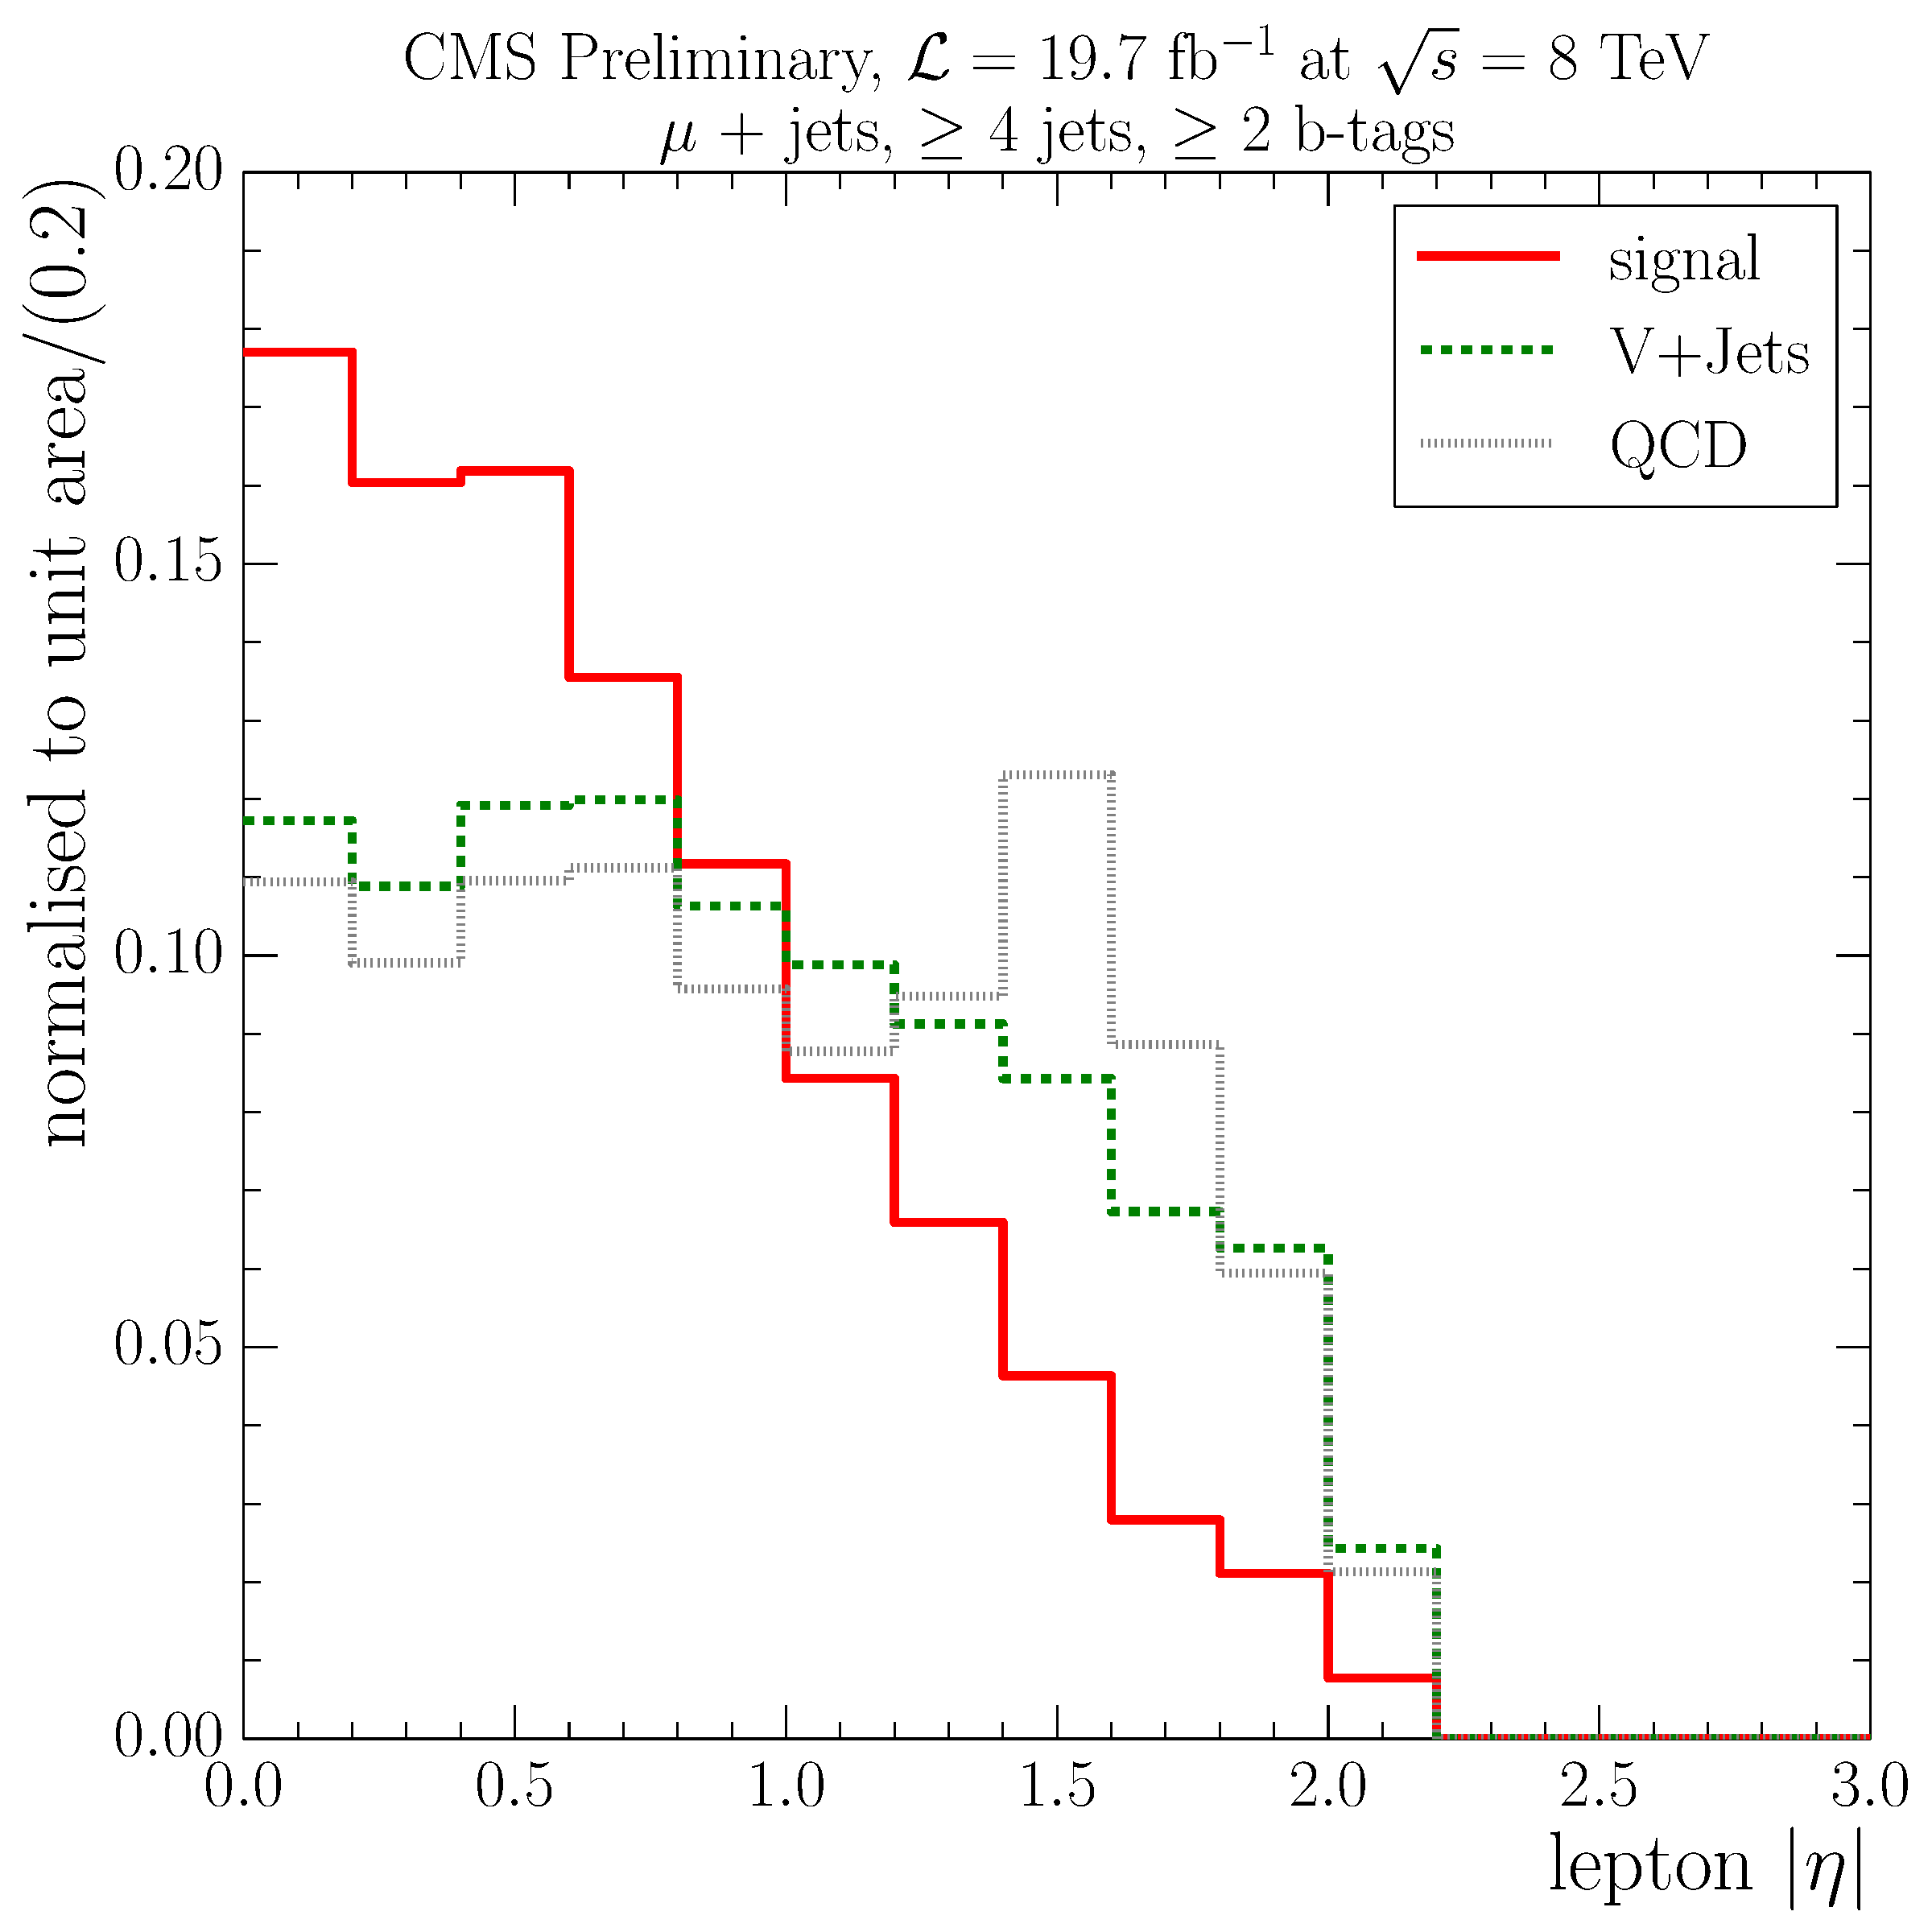
\includegraphics[width=0.39\textwidth]{measurement/WPT/central/fit_templates/muon_templates_bin_170-inf}}
    \hspace*{\fill}
    \caption[Muon $\abs \eta$ templates for the fit in different bins of \WPT]{Muon $\abs \eta$ templates for the fit
    in different bins of \WPT, from top left to bottom right: \SIrange{0}{40}{\GeV}, \SIrange{40}{70}{\GeV},
    \SIrange{70}{100}{\GeV}, \SIrange{100}{130}{\GeV}, \SIrange{130}{170}{\GeV} and $\geq \SI{170}{\GeV}$.}
    \label{fig:fit_templates_WPT_muon}
\end{figure}


\newpage
\section*{\MT variable}

\begin{figure}[!htbp]
  \centering
    \vspace*{-0.5cm}
    \hspace*{\fill}
    {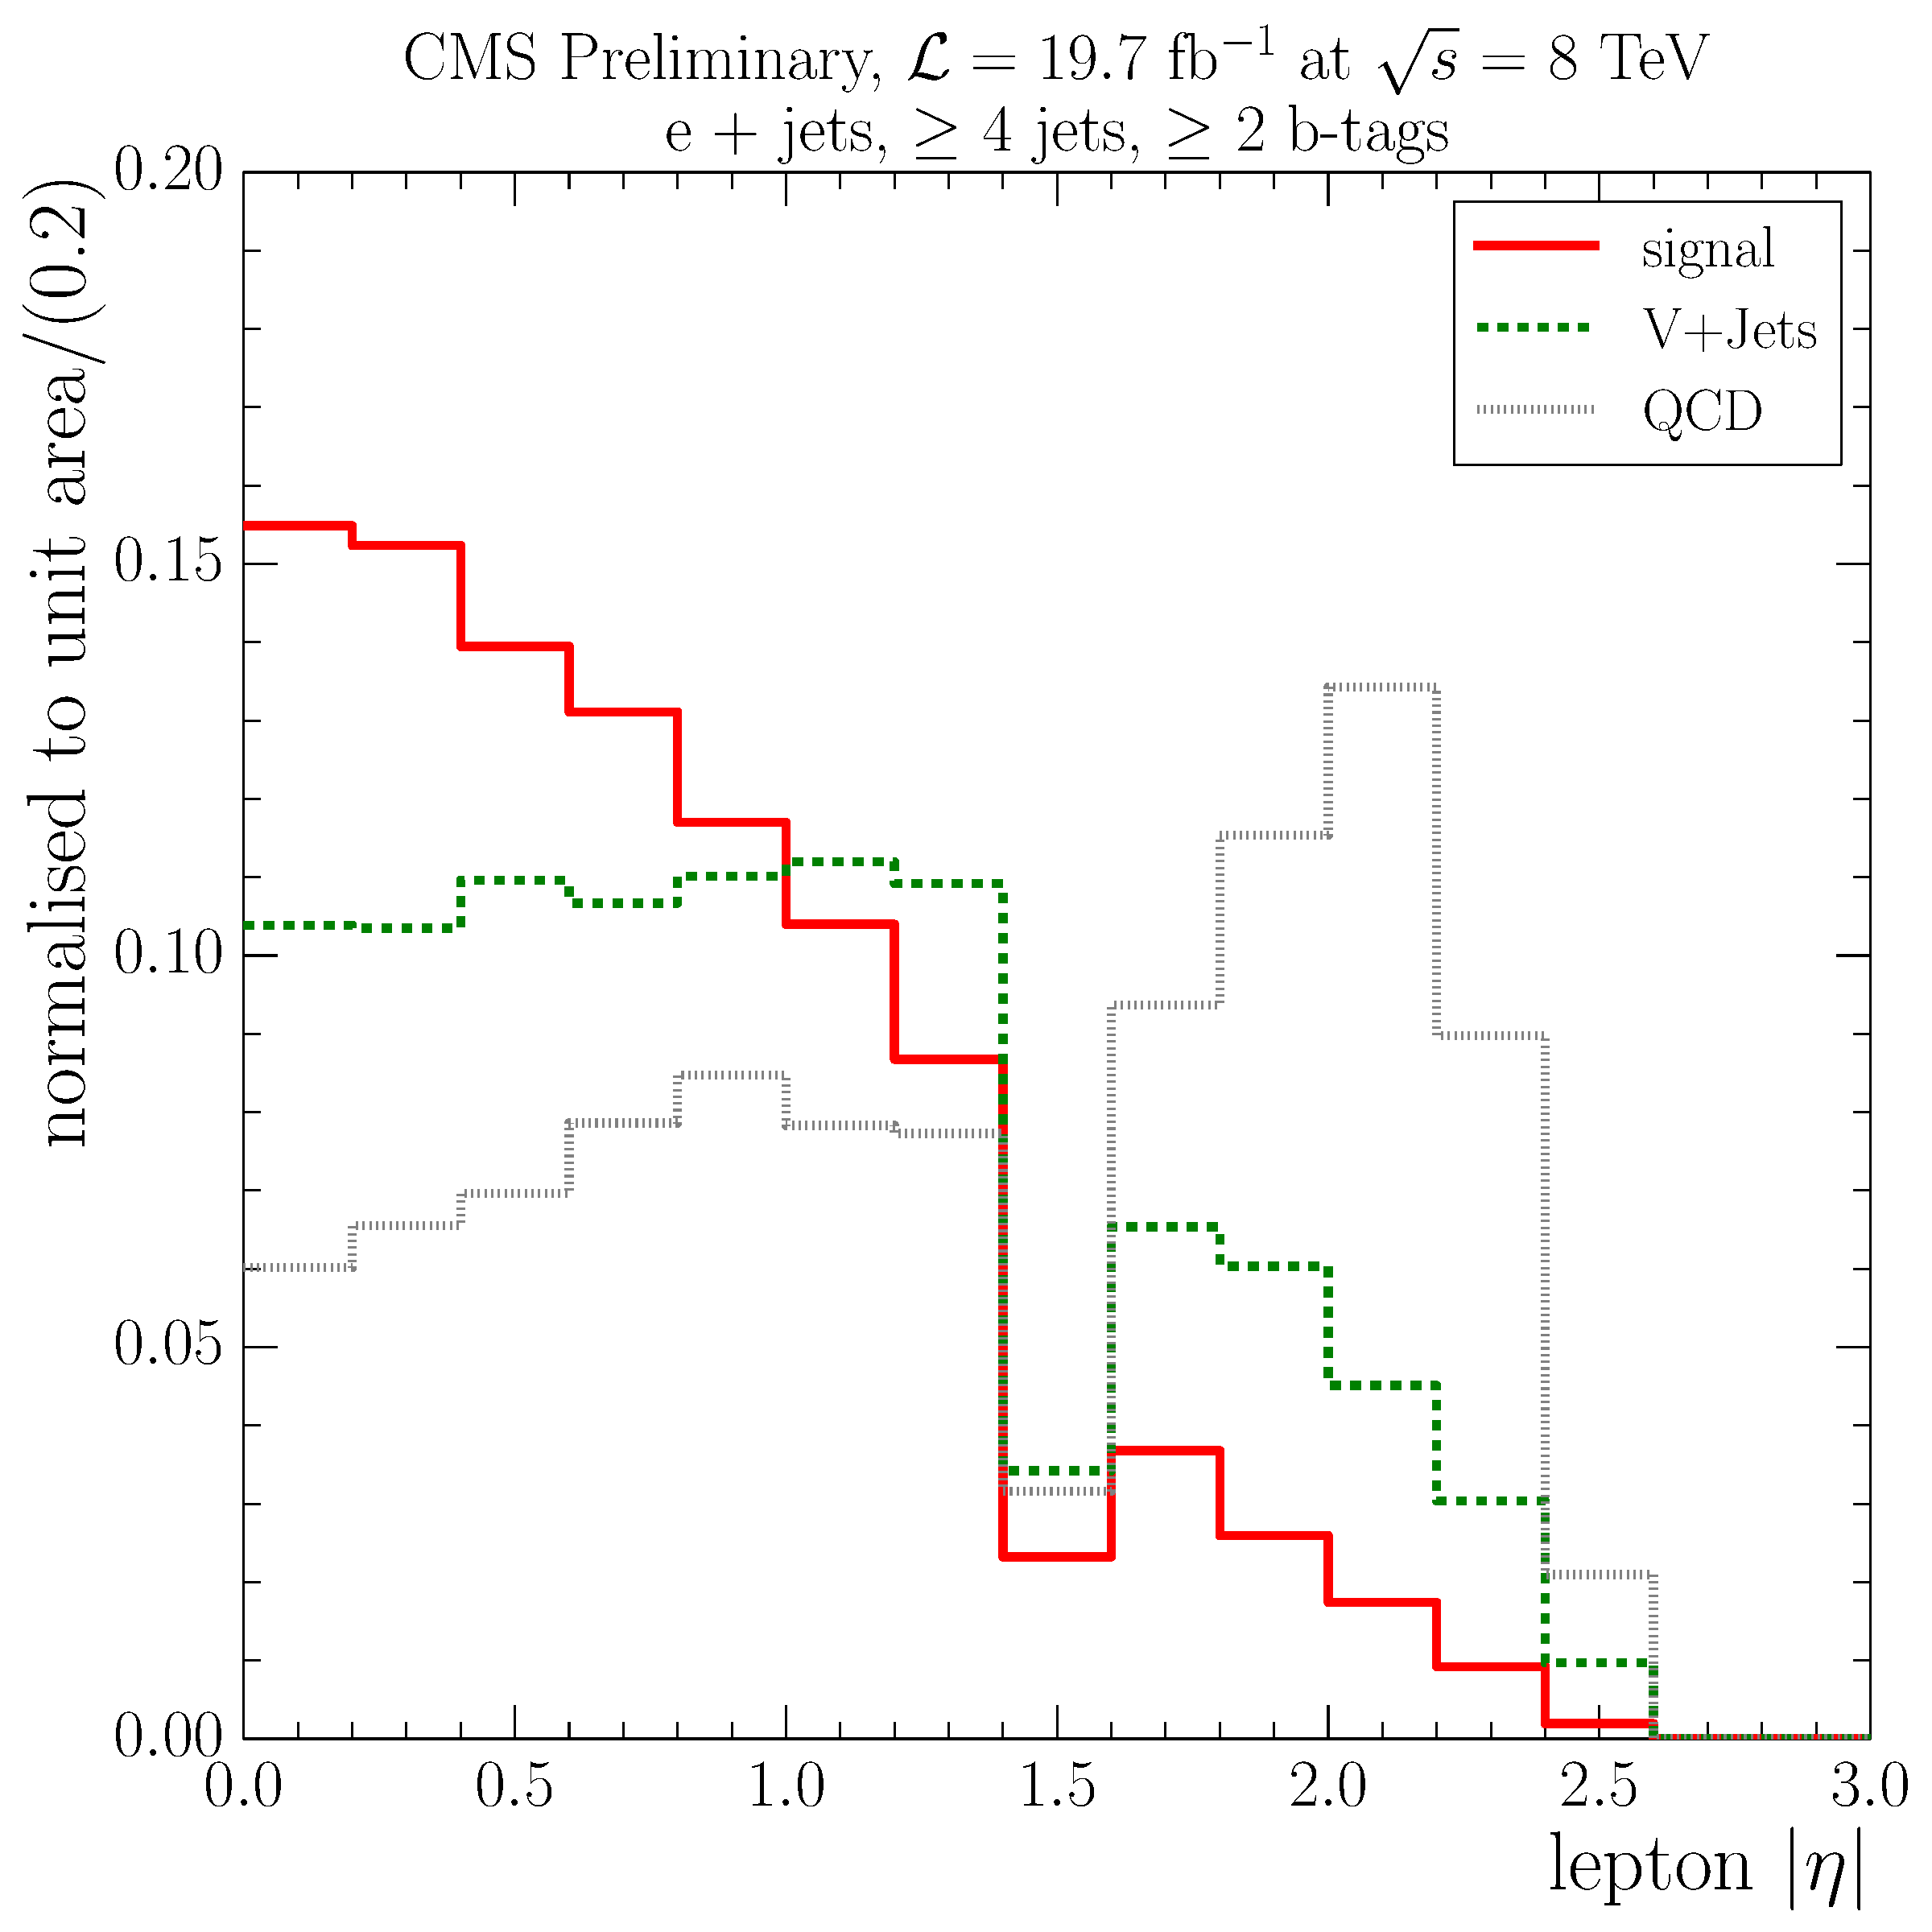
\includegraphics[width=0.39\textwidth]{measurement/MT/central/fit_templates/electron_templates_bin_0-30}}\hfill
    {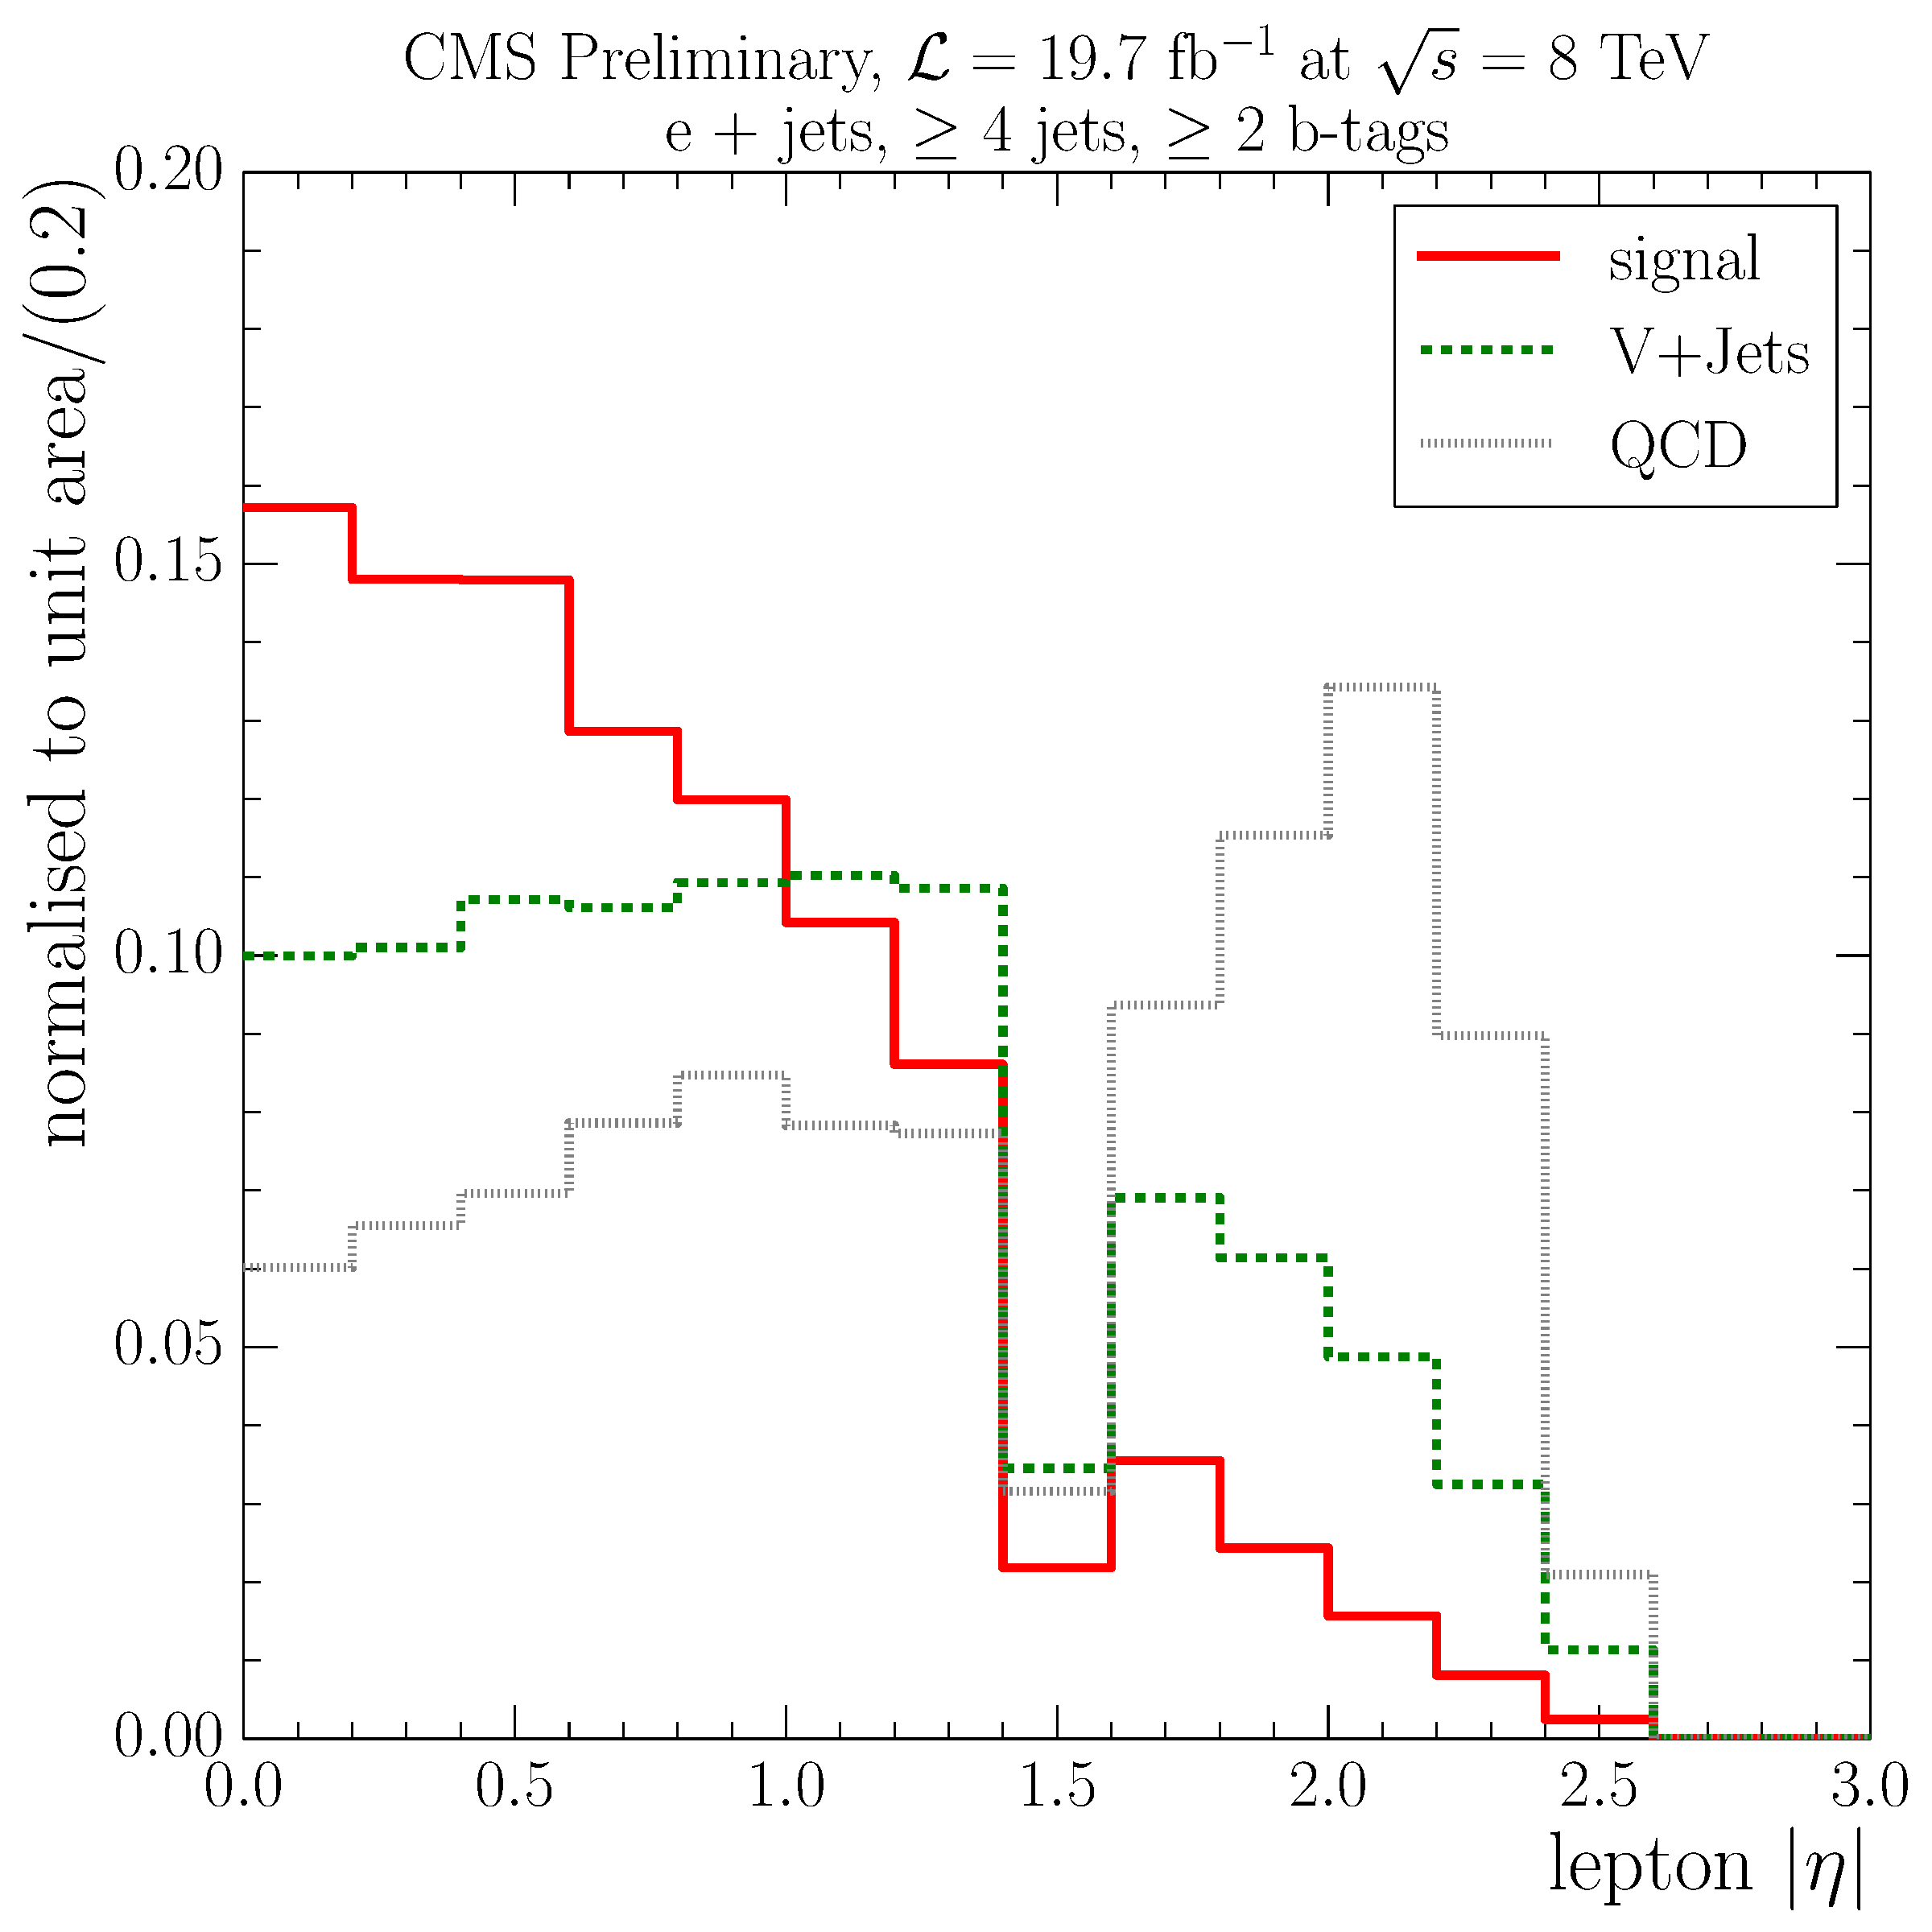
\includegraphics[width=0.39\textwidth]{measurement/MT/central/fit_templates/electron_templates_bin_30-50}}
    \hspace*{\fill} \\
    \hspace*{\fill}
    {\includegraphics[width=0.39\textwidth]{measurement/MT/central/fit_templates/electron_templates_bin_50-80}}\hfill
    {\includegraphics[width=0.39\textwidth]{measurement/MT/central/fit_templates/electron_templates_bin_80-100}}
    \hspace*{\fill} \\
    \hspace*{\fill}
    {\includegraphics[width=0.39\textwidth]{measurement/MT/central/fit_templates/electron_templates_bin_100-inf}}
    \hspace*{\fill}
    \caption[Electron $\abs \eta$ templates for the fit in different bins of \MT]{Electron $\abs \eta$ templates for the
    fit in different bins of \MT, from top left to bottom: \SIrange{0}{30}{\GeV}, \SIrange{30}{50}{\GeV},
    \SIrange{50}{80}{\GeV}, \SIrange{80}{100}{\GeV} and $\geq \SI{100}{\GeV}$.}
    \label{fig:fit_tempaltes_MT_electron}
\end{figure}

\begin{figure}[!htbp]
  \centering
    \hspace*{\fill}
    {\includegraphics[width=0.39\textwidth]{measurement/MT/central/fit_templates/muon_templates_bin_0-30}}\hfill
    {\includegraphics[width=0.39\textwidth]{measurement/MT/central/fit_templates/muon_templates_bin_30-50}}
    \hspace*{\fill} \\
    \hspace*{\fill}
    {\includegraphics[width=0.39\textwidth]{measurement/MT/central/fit_templates/muon_templates_bin_50-80}}\hfill
    {\includegraphics[width=0.39\textwidth]{measurement/MT/central/fit_templates/muon_templates_bin_80-100}}
    \hspace*{\fill} \\
    \hspace*{\fill}
    {\includegraphics[width=0.39\textwidth]{measurement/MT/central/fit_templates/muon_templates_bin_100-inf}}
    \hspace*{\fill}
    \caption[Muon $\abs \eta$ templates for the fit in different bins of \MT]{Muon $\abs \eta$ templates for the fit in
    different bins of \MT, from top left to bottom: \SIrange{0}{30}{\GeV}, \SIrange{30}{50}{\GeV},
    \SIrange{50}{80}{\GeV}, \SIrange{80}{100}{\GeV} and $\geq \SI{100}{\GeV}$.}
    \label{fig:fit_templates_MT_muon}
\end{figure}

\sisetup{range-phrase = {~to~}}
\sisetup{range-units = repeat}

\chapter{Systematic uncertainties}
\label{a:xsection_systematics_tables}

\begin{table}[htp]
	\centering
	\hspace*{-1cm}
	\caption{Systematic uncertainties for the normalised \ttbar cross section
	measurement with respect to \HT variable (combination of electron and muon channels). Dominating uncertainties are
	emphasised in bold.}
	\label{tab:combined_HT_systematics}
	\resizebox{\columnwidth}{!} {
	\begin{tabular}{_l^r^r^r^r^r^r^r}
	\toprule
	Systematic& 80--240~\GeV& 240--280~\GeV& 280--330~\GeV& 330--380~\GeV& 380--450~\GeV& 450--600~\GeV& $\geq 600$~\GeV \\
	\midrule
	Luminosity $+1\sigma$ (\%) & -0.00 & 0.00 & 0.01 & 0.01 & -0.00 & -0.02 & -0.03\\ 
	Luminosity $-1\sigma$ (\%) & 0.00 & -0.00 & -0.01 & -0.01 & 0.00 & 0.02 & 0.03\\ 
	\midrule
	Single top cross section $+1\sigma$ (\%) & -0.01 & 0.00 & 0.01 & 0.01 & 0.01 & 0.00 & -0.01\\ 
	Single top cross section $-1\sigma$ (\%) & 0.01 & -0.00 & -0.01 & -0.01 & -0.01 & -0.00 & 0.01\\ 
	$t\bar{t}$ cross section $+1\sigma$ (\%) & 0.01 & 0.00 & -0.01 & -0.01 & -0.01 & -0.00 & 0.01\\ 
	$t\bar{t}$ cross section $-1\sigma$ (\%) & -0.01 & 0.00 & 0.01 & 0.01 & 0.01 & 0.00 & -0.01\\ 
	\midrule
	b-tagging efficiency $+1\sigma$ (\%) & 0.01 & 0.02 & 0.02 & 0.01 & -0.01 & -0.06 & -0.10\\ 
	b-tagging efficiency $-1\sigma$ (\%) & 0.01 & -0.01 & -0.02 & -0.03 & -0.01 & 0.02 & 0.06\\ 
	\midrule
	b-tagging mis-tag rate $+1\sigma$ (\%) & 0.01 & 0.01 & 0.02 & 0.01 & -0.02 & -0.06 & -0.09\\ 
	b-tagging mis-tag rate $-1\sigma$ (\%) & 0.01 & -0.00 & -0.02 & -0.02 & -0.01 & 0.02 & 0.05\\ 
	\midrule
	Jet energy resolution $+1\sigma$ (\%) & 0.03 & -0.00 & -0.04 & -0.03 & -0.02 & -0.02 & 0.01\\ 
	Jet energy resolution $-1\sigma$ (\%) & -0.04 & -0.01 & 0.02 & 0.04 & 0.06 & 0.07 & 0.04\\ 
	\midrule
	Jet energy scale $+1\sigma$ (\%) \rowstyle{\bfseries} & -1.44 & -0.56 & 0.49 & 1.32 & 1.88 & 2.33 & 2.76\\ 
	Jet energy scale $-1\sigma$ (\%) \rowstyle{\bfseries} & 2.61 & 1.00 & -1.03 & -2.53 & -3.43 & -4.04 & -4.48\\ 
	\midrule
	Pile-up $+1\sigma$ (\%) & 0.07 & 0.02 & -0.03 & -0.08 & -0.11 & -0.09 & -0.04\\ 
	Pile-up $-1\sigma$ (\%) & -0.02 & -0.01 & 0.02 & 0.04 & 0.04 & 0.01 & -0.03\\ 
	\midrule
	QCD shape uncertainty (\%) & -0.21 & -0.07 & 0.10 & 0.26 & 0.32 & 0.27 & 0.14\\ 
	\midrule
	hadronisation uncertainty (\%) \rowstyle{\bfseries} & -1.76 & -4.78 & -1.22 & 2.07 & 6.27 & 9.07 & 6.02\\ 
	\midrule
	$p_\mathrm{T}(t,\bar{t})$ reweighting (\%) & 0.12 & 0.05 & -0.02 & -0.08 & -0.15 & -0.24 & -0.34\\ 
	\midrule
	$t\bar{t}$ (matching down) (\%) \rowstyle{\bfseries} & 2.71 & 0.25 & -1.39 & -2.33 & -3.49 & -3.51 & -2.20\\ 
	$t\bar{t}$ (matching up) (\%) & -0.11 & 0.16 & 0.17 & -0.26 & 0.55 & 0.46 & -1.76\\ 
	$t\bar{t}$ ($Q^{2}$ down) (\%) \rowstyle{\bfseries} & -5.42 & 1.94 & 3.50 & 3.98 & 4.33 & 4.78 & 3.23\\ 
	$t\bar{t}$ ($Q^{2}$ up) (\%) \rowstyle{\bfseries} & 4.05 & -1.62 & -2.75 & -2.86 & -2.68 & -3.54 & -2.74\\ 
	\midrule
	V+jets (matching down) (\%) & -0.45 & -0.22 & 0.12 & 0.26 & 0.42 & 1.02 & 1.38\\ 
	V+jets (matching up) (\%) & 0.41 & 0.07 & -0.24 & -0.45 & -0.41 & -0.38 & -0.60\\ 
	V+jets ($Q^{2}$ down) (\%) & -0.53 & -0.30 & 0.22 & 0.73 & 0.90 & 0.62 & 0.54\\ 
	V+jets ($Q^{2}$ up) (\%) & 0.52 & 0.31 & -0.13 & -0.63 & -0.96 & -0.88 & -0.56\\ 
	\midrule
	Electron energy $-1\sigma$ (\%) & 0.00 & 0.00 & 0.00 & 0.00 & 0.00 & 0.00 & 0.00\\ 
	Electron energy $+1\sigma$ (\%) & 0.00 & 0.00 & 0.00 & 0.00 & 0.00 & 0.00 & 0.00\\ 
	Muon energy $+1\sigma$ (\%) & 0.00 & 0.00 & 0.00 & 0.00 & 0.00 & 0.00 & 0.00\\ 
	Muon energy $-1\sigma$ (\%) & 0.00 & 0.00 & 0.00 & 0.00 & 0.00 & 0.00 & 0.00\\ 
	Tau energy $+1\sigma$ (\%) & 0.00 & 0.00 & 0.00 & 0.00 & 0.00 & 0.00 & 0.00\\ 
	Tau energy $-1\sigma$ (\%) & 0.00 & 0.00 & 0.00 & 0.00 & 0.00 & 0.00 & 0.00\\ 
	Unclustered energy $+1\sigma$ (\%) & 0.00 & 0.00 & 0.00 & 0.00 & 0.00 & 0.00 & 0.00\\ 
	Unclustered energy $-1\sigma$ (\%) & 0.00 & 0.00 & 0.00 & 0.00 & 0.00 & 0.00 & 0.00\\ 
	\midrule
	Total (\%) & 6.42  & 5.36  & 3.96  & 5.27  & 8.50  & 11.19  & 8.59 \\ 
	\bottomrule
	\end{tabular}
}
\end{table}
\begin{table}[htp]
	\centering
	\hspace*{-1cm}
	\caption[Systematic uncertainties for the normalised \ttbar cross section measurement with respect to
	\ST]{Systematic uncertainties for the normalised \ttbar cross section measurement with respect to \ST variable
	(combination of electron and muon channels). Dominating uncertainties are emphasised in bold.}
	\label{tab:combined_ST_systematics}
	\resizebox{\columnwidth}{!} {
	\begin{tabular}{@{}_l^r^r^r^r^r^r^r@{}}
	\toprule
	Systematic& 106--350~\GeV& 350--400~\GeV& 400--450~\GeV& 450--500~\GeV& 500--580~\GeV& 580--700~\GeV& $\geq 700$~\GeV \\
	\midrule
	Luminosity $+1\sigma$ (\%) & -0.01 & 0.00 & 0.01 & 0.01 & 0.01 & 0.00 & -0.01\\ 
	Luminosity $-1\sigma$ (\%) & 0.01 & -0.00 & -0.01 & -0.01 & -0.01 & -0.00 & 0.01\\ 
	\midrule
	Single top cross section $+1\sigma$ (\%) & -0.00 & 0.00 & 0.01 & 0.01 & 0.00 & -0.01 & -0.02\\ 
	Single top cross section $-1\sigma$ (\%) & 0.00 & -0.00 & -0.01 & -0.01 & -0.00 & 0.01 & 0.02\\ 
	$t\bar{t}$ cross section $+1\sigma$ (\%) & 0.00 & -0.00 & -0.01 & -0.01 & -0.00 & 0.01 & 0.02\\ 
	$t\bar{t}$ cross section $-1\sigma$ (\%) & -0.00 & 0.00 & 0.01 & 0.01 & 0.00 & -0.01 & -0.03\\ 
	\midrule
	b-tagging efficiency $+1\sigma$ (\%) & 0.00 & 0.01 & 0.02 & 0.01 & -0.01 & -0.04 & -0.07\\ 
	b-tagging efficiency $-1\sigma$ (\%) & 0.03 & -0.00 & -0.03 & -0.05 & -0.04 & -0.02 & 0.02\\ 
	\midrule
	b-tagging mis-tag rate $+1\sigma$ (\%) & 0.00 & 0.01 & 0.02 & 0.02 & -0.01 & -0.04 & -0.06\\ 
	b-tagging mis-tag rate $-1\sigma$ (\%) & 0.03 & 0.00 & -0.03 & -0.04 & -0.04 & -0.03 & 0.00\\ 
	\midrule
	Jet energy resolution $+1\sigma$ (\%) & 0.09 & 0.02 & -0.08 & -0.13 & -0.12 & -0.09 & -0.04\\ 
	Jet energy resolution $-1\sigma$ (\%) & -0.04 & 0.01 & 0.03 & 0.03 & 0.04 & 0.03 & 0.02\\ 
	\midrule
	Jet energy scale $+1\sigma$ (\%) \rowstyle{\bfseries} & -1.12 & -0.42 & 0.35 & 0.97 & 1.56 & 2.23 & 2.77\\ 
	Jet energy scale $-1\sigma$ (\%) \rowstyle{\bfseries} & 2.18 & 0.77 & -1.03 & -2.38 & -3.20 & -3.71 & -4.02\\ 
	\midrule
	Pile-up $+1\sigma$ (\%) & 0.06 & 0.01 & -0.04 & -0.08 & -0.10 & -0.09 & -0.04\\ 
	Pile-up $-1\sigma$ (\%) & -0.00 & 0.00 & 0.01 & 0.01 & 0.01 & -0.02 & -0.05\\ 
	\midrule
	QCD shape uncertainty (\%) & -0.23 & -0.03 & 0.21 & 0.34 & 0.33 & 0.21 & 0.04\\ 
	\midrule
	hadronisation uncertainty (\%) \rowstyle{\bfseries} & -0.75 & -5.16 & -1.90 & 1.56 & 5.50 & 8.35 & 6.14\\ 
	\midrule
	$p_\mathrm{T}(t,\bar{t})$ reweighting (\%) & 0.11 & 0.09 & 0.02 & -0.09 & -0.20 & -0.30 & -0.40\\ 
	\midrule
	$t\bar{t}$ (matching down) (\%) \rowstyle{\bfseries} & 2.06 & -0.22 & -1.34 & -1.88 & -2.47 & -2.39 & -2.59\\ 
	$t\bar{t}$ (matching up) (\%) & -0.29 & 0.20 & 0.58 & -0.05 & 0.66 & 0.68 & -1.57\\ 
	$t\bar{t}$ ($Q^{2}$ down) (\%) \rowstyle{\bfseries} & -5.02 & 2.83 & 3.98 & 3.42 & 4.58 & 4.66 & 2.73\\ 
	$t\bar{t}$ ($Q^{2}$ up) (\%) \rowstyle{\bfseries} & 3.39 & -1.86 & -2.59 & -3.05 & -2.18 & -2.83 & -2.89\\ 
	\midrule
	V+jets (matching down) (\%) & -0.14 & -0.08 & -0.07 & -0.10 & 0.07 & 0.54 & 1.01\\ 
	V+jets (matching up) (\%) & 0.60 & 0.12 & -0.43 & -0.72 & -0.75 & -0.77 & -0.86\\ 
	V+jets ($Q^{2}$ down) (\%) & -0.38 & -0.36 & 0.01 & 0.55 & 0.80 & 0.88 & 0.96\\ 
	V+jets ($Q^{2}$ up) (\%) & 0.53 & 0.19 & -0.24 & -0.57 & -0.84 & -1.00 & -0.82\\ 
	\midrule
	Electron energy $-1\sigma$ (\%) & 0.02 & -0.00 & -0.04 & -0.04 & -0.02 & 0.01 & 0.01\\ 
	Electron energy $+1\sigma$ (\%) & 0.01 & 0.02 & 0.01 & 0.00 & -0.03 & -0.07 & -0.09\\ 
	Muon energy $-1\sigma$ (\%) & -0.01 & -0.01 & -0.01 & 0.00 & 0.02 & 0.03 & 0.03\\ 
	Muon energy $+1\sigma$ (\%) & 0.02 & 0.00 & -0.01 & -0.02 & -0.03 & -0.02 & -0.01\\ 
	Tau energy $-1\sigma$ (\%) & 0.00 & -0.00 & -0.01 & -0.01 & -0.00 & 0.01 & 0.02\\ 
	Tau energy $+1\sigma$ (\%) & 0.00 & -0.00 & -0.00 & -0.01 & -0.00 & 0.00 & 0.01\\ 
	Unclustered energy $-1\sigma$ (\%) & 0.20 & 0.09 & -0.07 & -0.23 & -0.34 & -0.37 & -0.35\\ 
	Unclustered energy $+1\sigma$ (\%) & -0.20 & -0.09 & 0.06 & 0.22 & 0.34 & 0.40 & 0.39\\ 
	\midrule
	Total (\%) & 5.70  & 6.02  & 4.67  & 4.75  & 8.00  & 10.40  & 8.62 \\ 
	\bottomrule
	\end{tabular}
}
\end{table}
\begin{table}[htp]
	\centering
	\hspace*{-1cm}
	\caption[Systematic uncertainties for the normalised \ttbar cross section measurement with respect to
	\MT]{Systematic uncertainties for the normalised \ttbar cross section measurement with respect to \MT variable
	(combination of electron and muon channels). Dominating uncertainties are emphasised in bold.}
	\label{tab:combined_MT_systematics}
	\resizebox{\columnwidth}{!} {
	\begin{tabular}{@{}_l^r^r^r^r^r@{}}
	\toprule
	Systematic& 0--30~\GeV& 30--50~\GeV& 50--80~\GeV& 80--100~\GeV& $\geq 100$~\GeV \\
	\midrule
	Luminosity $+1\sigma$ (\%) & -0.01 & -0.01 & 0.00 & 0.01 & 0.02\\ 
	Luminosity $-1\sigma$ (\%) & 0.01 & 0.01 & -0.00 & -0.01 & -0.02\\ 
	\midrule
	Single top cross section $+1\sigma$ (\%) & 0.00 & 0.00 & -0.00 & -0.00 & -0.01\\ 
	Single top cross section $-1\sigma$ (\%) & -0.00 & -0.00 & 0.00 & 0.00 & 0.01\\ 
	$t\bar{t}$ cross section $+1\sigma$ (\%) & -0.00 & -0.00 & 0.00 & 0.00 & 0.01\\ 
	$t\bar{t}$ cross section $-1\sigma$ (\%) & 0.01 & 0.00 & -0.00 & -0.00 & -0.01\\ 
	\midrule
	b-tagging efficiency $+1\sigma$ (\%) & -0.02 & -0.01 & 0.00 & 0.02 & 0.03\\ 
	b-tagging efficiency $-1\sigma$ (\%) & 0.04 & 0.02 & -0.00 & -0.04 & -0.08\\ 
	\midrule
	b-tagging mis-tag rate $+1\sigma$ (\%) & -0.01 & -0.01 & 0.00 & 0.01 & 0.01\\ 
	b-tagging mis-tag rate $-1\sigma$ (\%) & 0.02 & 0.02 & -0.00 & -0.03 & -0.06\\ 
	\midrule
	Jet energy resolution $+1\sigma$ (\%) & -0.03 & -0.01 & 0.01 & 0.00 & -0.02\\ 
	Jet energy resolution $-1\sigma$ (\%) & -0.04 & -0.01 & 0.01 & 0.02 & 0.03\\ 
	\midrule
	Jet energy scale $+1\sigma$ (\%) \rowstyle{\bfseries} & 0.77 & 0.40 & -0.14 & -0.62 & -0.93\\ 
	Jet energy scale $-1\sigma$ (\%) \rowstyle{\bfseries} & -0.93 & -0.48 & 0.17 & 0.75 & 1.15\\ 
	\midrule
	Pile-up $+1\sigma$ (\%) & 0.01 & 0.01 & 0.00 & -0.03 & -0.06\\ 
	Pile-up $-1\sigma$ (\%) & 0.05 & 0.02 & -0.01 & -0.03 & -0.03\\ 
	\midrule
	QCD shape uncertainty (\%) & -0.21 & -0.12 & 0.04 & 0.18 & 0.28\\ 
	\midrule
	hadronisation uncertainty (\%) \rowstyle{\bfseries} & 2.37 & 1.07 & -0.74 & 0.34 & -8.82\\ 
	\midrule
	$p_\mathrm{T}(t,\bar{t})$ reweighting (\%) & 0.34 & 0.17 & -0.07 & -0.25 & -0.35\\ 
	\midrule
	$t\bar{t}$ (matching down) (\%) & -0.26 & -0.07 & 0.08 & 0.21 & -1.24\\ 
	$t\bar{t}$ (matching up) (\%) & 0.17 & -0.43 & -0.02 & 0.57 & -1.34\\ 
	$t\bar{t}$ ($Q^{2}$ down) (\%) \rowstyle{\bfseries} & 2.09 & 0.38 & -0.37 & -0.70 & -4.05\\ 
	$t\bar{t}$ ($Q^{2}$ up) (\%) \rowstyle{\bfseries} & -1.20 & -0.89 & 0.29 & 0.95 & 1.61\\ 
	\midrule
	V+jets (matching down) (\%) \rowstyle{\bfseries} & -0.96 & -0.53 & 0.17 & 0.82 & 1.25\\ 
	V+jets (matching up) (\%) & 0.16 & 0.05 & -0.05 & -0.05 & -0.02\\ 
	V+jets ($Q^{2}$ down) (\%) \rowstyle{\bfseries} & 0.87 & 0.43 & -0.18 & -0.61 & -0.81\\ 
	V+jets ($Q^{2}$ up) (\%) & 0.12 & 0.17 & 0.06 & -0.43 & -0.99\\ 
	\midrule
	Electron energy $+1\sigma$ (\%) & -0.91 & -0.52 & 0.14 & 0.86 & 1.42\\ 
	Electron energy $-1\sigma$ (\%) & 0.82 & 0.46 & -0.13 & -0.75 & -1.21\\ 
	Muon energy $+1\sigma$ (\%) & -0.25 & -0.14 & 0.04 & 0.22 & 0.34\\ 
	Muon energy $-1\sigma$ (\%) & 0.30 & 0.16 & -0.05 & -0.26 & -0.42\\ 
	Tau energy $+1\sigma$ (\%) & -0.00 & -0.00 & 0.00 & 0.01 & 0.01\\ 
	Tau energy $-1\sigma$ (\%) & -0.01 & -0.01 & 0.00 & 0.02 & 0.04\\ 
	Unclustered energy $+1\sigma$ (\%) & 0.54 & 0.28 & -0.11 & -0.40 & -0.54\\ 
	Unclustered energy $-1\sigma$ (\%) & -0.74 & -0.39 & 0.14 & 0.58 & 0.82\\ 
	\midrule
	Total (\%) & 3.89  & 2.02  & 1.10  & 2.10  & 10.23 \\ 
	\bottomrule
	\end{tabular}
}
\end{table}
\begin{table}[htp]
	\centering
	\hspace*{-1cm}
	\caption[Systematic uncertainties for the normalised \ttbar cross section measurement with respect to
	\WPT]{Systematic uncertainties for the normalised \ttbar cross section measurement with respect to \WPT variable
	(combination of electron and muon channels). Dominating uncertainties are emphasised in bold.}
	\label{tab:combined_WPT_systematics}
	\resizebox{\columnwidth}{!} {
	\begin{tabular}{@{}_l^r^r^r^r^r^r@{}}
	\toprule
	Systematic& 0--40~\GeV& 40--70~\GeV& 70--100~\GeV& 100--130~\GeV& 130--170~\GeV& $\geq 170$~\GeV \\
	\midrule
	Luminosity $+1\sigma$ (\%) & -0.02 & -0.01 & 0.01 & 0.02 & 0.01 & -0.01\\ 
	Luminosity $-1\sigma$ (\%) & 0.02 & 0.01 & -0.01 & -0.02 & -0.01 & 0.01\\ 
	\midrule
	Single top cross section $+1\sigma$ (\%) & 0.01 & 0.01 & 0.01 & -0.00 & -0.02 & -0.05\\ 
	Single top cross section $-1\sigma$ (\%) & -0.01 & -0.01 & -0.01 & 0.00 & 0.02 & 0.05\\ 
	$t\bar{t}$ cross section $+1\sigma$ (\%) & -0.01 & -0.01 & -0.01 & 0.00 & 0.03 & 0.06\\ 
	$t\bar{t}$ cross section $-1\sigma$ (\%) & 0.01 & 0.01 & 0.01 & -0.01 & -0.03 & -0.06\\ 
	\midrule
	b-tagging efficiency $+1\sigma$ (\%) & 0.02 & -0.00 & -0.01 & 0.01 & -0.00 & -0.04\\ 
	b-tagging efficiency $-1\sigma$ (\%) & 0.05 & 0.02 & -0.03 & -0.06 & -0.04 & 0.01\\ 
	\midrule
	b-tagging mis-tag rate $+1\sigma$ (\%) & 0.01 & -0.00 & -0.00 & 0.01 & -0.00 & -0.04\\ 
	b-tagging mis-tag rate $-1\sigma$ (\%) & 0.06 & 0.02 & -0.03 & -0.06 & -0.03 & 0.02\\ 
	\midrule
	Jet energy resolution $+1\sigma$ (\%) & 0.06 & 0.02 & -0.03 & -0.04 & -0.02 & -0.00\\ 
	Jet energy resolution $-1\sigma$ (\%) & -0.00 & -0.03 & -0.03 & 0.00 & 0.07 & 0.14\\ 
	\midrule
	Jet energy scale $+1\sigma$ (\%) \rowstyle{\bfseries} & -1.23 & -0.74 & 0.09 & 0.97 & 1.66 & 2.15\\ 
	Jet energy scale $-1\sigma$ (\%) \rowstyle{\bfseries} & 1.13 & 0.75 & 0.04 & -0.86 & -1.74 & -2.49\\ 
	\midrule
	Pile-up $+1\sigma$ (\%) & 0.11 & 0.04 & -0.04 & -0.07 & -0.08 & -0.10\\ 
	Pile-up $-1\sigma$ (\%) & -0.02 & -0.01 & 0.00 & 0.00 & 0.02 & 0.07\\ 
	\midrule
	QCD shape uncertainty (\%) & -0.42 & -0.24 & 0.09 & 0.38 & 0.48 & 0.46\\ 
	\midrule
	hadronisation uncertainty (\%) \rowstyle{\bfseries} & -1.28 & 1.46 & -0.53 & -1.99 & 1.06 & 2.41\\ 
	\midrule
	$p_\mathrm{T}(t,\bar{t})$ reweighting (\%) & 0.24 & 0.19 & 0.05 & -0.17 & -0.45 & -0.72\\ 
	\midrule
	$t\bar{t}$ (matching up) (\%) & 0.49 & -0.14 & -0.09 & -0.21 & 0.15 & -0.32\\ 
	$t\bar{t}$ (matching down) (\%) & 0.15 & 0.50 & 0.27 & -0.82 & -0.82 & -0.63\\ 
	$t\bar{t}$ ($Q^{2}$ up) (\%) & 0.43 & 0.19 & 0.04 & -0.61 & -0.74 & 0.12\\ 
	$t\bar{t}$ ($Q^{2}$ down) (\%) & 0.93 & 0.34 & -0.34 & -0.95 & -0.14 & -0.80\\ 
	\midrule
	V+jets (matching up) (\%) & 0.24 & 0.12 & 0.01 & -0.08 & -0.28 & -0.72\\ 
	V+jets (matching down) (\%) \rowstyle{\bfseries} & 1.06 & 0.36 & -0.35 & -0.73 & -0.84 & -0.75\\ 
	V+jets ($Q^{2}$ up) (\%) & -0.04 & 0.25 & 0.24 & -0.23 & -0.53 & -0.55\\ 
	V+jets ($Q^{2}$ down) (\%) & -0.62 & -0.16 & 0.32 & 0.46 & 0.24 & 0.07\\ 
	\midrule
	Electron energy $+1\sigma$ (\%) & 0.27 & 0.16 & 0.01 & -0.16 & -0.39 & -0.65\\ 
	Electron energy $-1\sigma$ (\%) & -0.36 & -0.16 & 0.06 & 0.23 & 0.39 & 0.53\\ 
	Muon energy $+1\sigma$ (\%) & 0.10 & 0.07 & 0.01 & -0.07 & -0.16 & -0.26\\ 
	Muon energy $-1\sigma$ (\%) & -0.09 & -0.05 & -0.00 & 0.04 & 0.12 & 0.23\\ 
	Tau energy $+1\sigma$ (\%) & 0.00 & -0.01 & -0.02 & -0.00 & 0.03 & 0.06\\ 
	Tau energy $-1\sigma$ (\%) & 0.01 & 0.00 & 0.01 & 0.00 & -0.02 & -0.03\\ 
	Unclustered energy $+1\sigma$ (\%) & -0.92 & -0.55 & 0.04 & 0.67 & 1.26 & 1.79\\ 
	Unclustered energy $-1\sigma$ (\%) & 0.82 & 0.51 & -0.00 & -0.59 & -1.18 & -1.78\\ 
	\midrule
	Total (\%) & 2.75  & 2.10  & 1.11  & 2.92  & 3.02  & 4.48 \\ 
	\bottomrule
	\end{tabular}
}
\end{table}

%%% Local Variables: 
%%% mode: latex
%%% TeX-master: "../thesis"
%%% End: 
